\documentclass{book} 
\usepackage{amsmath}
\usepackage{enumerate}
\usepackage{amssymb}
\usepackage{ctex}
\usepackage{graphicx}
\usepackage[linesnumbered,ruled,algochapter]{algorithm2e}
\renewcommand{\algorithmcfname}{算法}
\usepackage{titlesec}
\usepackage{amsthm}
\usepackage{indentfirst}
\usepackage{geometry}
\geometry{left=2.5cm,right=2.5cm}
\usepackage{chapterbib}
\usepackage{fancyhdr}
\usepackage{makeidx}
\usepackage{tikz-cd}
\makeindex
\pagestyle{plain}
\newtheorem{dfn}{定义}[chapter]
\newtheorem{axi}[dfn]{公理}
\newtheorem{thm}[dfn]{定理}
\newtheorem{pro}[dfn]{命题}
\newtheorem{lem}[dfn]{引理}
\newtheorem{col}[dfn]{推论}


\begin{document}
\pagenumbering{Roman}
\setlength{\parindent}{0em}
\Large

\title{\Huge{\textbf{自怡数学手册}} \\ \vspace{0.5cm} \huge{Ziyi Handbook of Mathematics}}  %%书名
\author{\Large{郭浩\, 编著}} %%作者
\date{\Large{\today}}

\maketitle
\large

\renewcommand{\contentsname}{\centerline{目录}}
\tableofcontents  %%生成目录

\pagenumbering{arabic}

\mainmatter %%表示文章的正文部分，在生成目录后将从第一页开始
\chapter*{前言}
\addcontentsline{toc}{chapter}{前言}

\par \emph{In order to understand the universe, you must know the language in which it is written. And that language is mathematics.} 
\par \rightline{——Galileo Galilei}

\par \emph{Curiosity is part of human nature. Unfortunately, the established religions no longer provide the answers that are satisfactory, and that translates into a need for certainty and truth. And that is what makes mathematics work, makes people commit their lives to it. It is the desire for truth and the response to the beauty and elegance of mathematics that drives mathematicians.}
\par \rightline{——Landon Clay}

\par \emph{It is at the higher and apical levels of geometry, topology, analysis, number theory and mathematical logic that the fun and profundity start.}
\par \rightline{——David Foster Wallace}

\par \emph{Having tasted the pleasure in mathematics he will not forget it easily and then there is a good chance that mathematics will become something for him: a hobby, or a tool of his profession, or his profession, or a great ambition.}
\par \rightline{——George Pólya}

\par \emph{The only way to learn mathematics is to do mathematics.} \par \rightline{——Paul Halmos}

\section*{我与数学的缘分}

\section*{数学的意义}

\section*{编写目的和原则}

\section*{内容编排}


\part{数学基础}
\chapter{数理逻辑}
\chapter{集合}

\par \emph{道生一，一生二，二生三，三生万物.} 
\par \rightline{——《老子》}

\par \emph{汤问棘曰:``上下四方有极乎?''\\ 棘曰:``无极之外, 复无极也.''}
\par \rightline{——《庄子·逍遥游》}

\section{Zermelo-Fraenkel公理系统}

\par ZFC公理系统由Zermelo-Fraenkel系统的八条公理和选择公理构成. 

\par 公理集合论不定义“集合”，而是界定允许对集合进行的操作. 同样不定义“属于”，元素$x$属于集合$A$记作$x\in A$, 此时称$A$包含$x$.

\begin{dfn} \textbf{子集} Subset\\
设$A,B$是集合, 若$\forall x \in A: x \in B$, 称$A$是$B$的子集, 记作$A\subseteq B$. 
\end{dfn}

\begin{axi} \textbf{外延公理} Axiom of Extension\\
设$A,B$是集合，则$A=B$当且仅当$A\subseteq B$且$B\subseteq A$. 
\end{axi}
\par 外延公理用自然语言表述为，两个集合相等当且仅当它们包含相同的元素. 这意味着集合完全由它们包含的元素（外延）确定. 

\par 给定全集$E$, $\subseteq$是$\mathcal{P}(E)$上的偏序关系. 事实上, 外延公理表明$\subseteq$是反对称的，而根据定义$\subseteq$是自反的、传递的. 同理，$=$是$\mathcal{P}(E)$上的等价关系. 事实上, 外延公理表明集合间的相等关系$=$是自反的、对称的，而$\subseteq$的传递性蕴含$=$的传递性.

\begin{dfn} \textbf{真子集}\\
设$A,B$是集合，若$A\subseteq B$且$A\neq B$，称$A$是$B$的真子集，记作$A\subset B$. 
\end{dfn}

\begin{axi} \textbf{分类公理模式} Axiom of Specification\\
设$A$是集合，$S(x)$是条件，则$A$中$S(x)$的所有元素构成集合$B$，记作$B=\{x\in A\vert S(x)\}$. 
\end{axi}
其中条件$S(x)$指含自由变元$x$的语句. 语句由逻辑运算符($\land, \lor, \lnot, \Rightarrow, \Leftrightarrow, \forall, \exists$)连接原子语句（属于、相等）得到. 

\begin{col}\textbf{空集存在}\\
设至少存在一个集合，则存在不包含任何元素的集合，称为空集$\varnothing$.
\end{col}
\begin{proof}
    设$A$是集合，令$\varnothing=\{x\in A\vert x\neq x\}$. 
\end{proof} 

\begin{col}\textbf{不存在包含一切的集合}\\
设$A$是集合，则存在$B \notin A$.
\end{col}
\begin{proof}
    令$B=\{x\in A\vert x\notin x\}$, 用反证法，假设$B\in A$，则$B\notin B\Rightarrow B\in B$，$B\in B\Rightarrow B\notin B$，均导致矛盾. 故$B\notin A$. 
\end{proof}
若分类公理模式不加入$x\in A$的限定，允许定义集合$B=\{x\vert x\notin x\}$，类似的推理将导致Russell悖论.

\begin{axi} \textbf{无序对公理} Axiom of Pairing\\
设$a,b$是集合，存在集合$A$满足$a\in A$且 $b \in A$. 
\end{axi}
无序对公理的一个等价叙述是：设$a,b$是集合，存在一个集合恰好包含$a, b$, 称为$a,b$的无序对(unordered pair), 记作$\{a,b\}$. 事实上，设$a,b \in A$, 基于分类公理模式可令$\{a,b\}=\{x\in A\vert x=a \lor x=b\}$. 设$a$是集合，无序对公理还表明存在集合$\{a,a\}=\{a\}$，称为$a$的单件(singleton).

\begin{axi} \textbf{并集公理} Axiom of Unions\\
设$\mathcal{C}$是集合的集合(或称集族)，则存在集合$U$，满足对任意$x$，若存在$X\in \mathcal{C}$，$x\in X$，则$x\in U$. 
\end{axi}
并集公理也断言存在一个集合恰好由属于$\mathcal{C}$中至少一个集合的元素构成，称为$\mathcal{C}$中集合的并集，记作$\bigcup_{X\in \mathcal{C}}X$. 对$\mathcal{C}=\{A,B\}$的情形，并集记作$A\cup B=\{x|x\in A \lor x\in B\}$.

\begin{axi} \textbf{幂集公理} Axiom of Powers\\
设$E$是集合，则存在集族$\mathcal{P}$，满足对任意$X\subseteq E$，$x\in \mathcal{P}$. 
\end{axi}
幂集公理也断言存在一个集合恰好由$E$的全部子集构成，称为$E$的幂集，记作$\mathcal{P}(E)=\{X\vert X\subseteq E\}$.

\begin{axi} \textbf{无穷公理} Axiom of Infinity\\
存在集合$A$, 满足$\varnothing \in A$, 且$\forall x\in A : x\cup \{x\} \in A$.
\end{axi}
$x\cup \{x\}$称为$x$的后继(sucessor), 记作$x^{+}$.

\begin{axi} \textbf{替换公理模式} Axiom of Substitution\\
设$A$是集合，$S(a,b)$是条件，若对$\forall a\in A$, 存在集合$\{b\vert S(a,b)\}$, 则存在定义域为$A$的函数$F$满足$\forall a\in A: F(a)=\{b\vert S(a,b)\}$. 
\end{axi}

\begin{axi} \textbf{正则性公理} Axiom of Regularity\\
设$A$是非空集合, 存在$a\in A$且$a\cap A=\varnothing$. 
\end{axi}

\begin{col}\textbf{集合不能包含自身}\\
设$A, B$是集合，则$A\notin A$，且$A\notin B\lor B\notin A$.
\label{col:self_inclusion}
\end{col}
\begin{proof}
不妨设$A$非空, 由无序对公理, 存在$\{A\}$和$\{A,B\}$. 若$A\in A$, 或$A\in B\land B\in A$, 与正则性公理矛盾. 
\end{proof}

\section{集合的运算}

\begin{pro} \textbf{交集} Intersection\\
设$\mathcal{C}$是非空集族，则存在集合$V$，满足$x\in V$当且仅当对任意$X\in \mathcal{C}$，$x\in X$. 
\end{pro}
\begin{proof}
    设$A\in \mathcal{C}$，令$V=\{x\in A\vert \forall X\in \mathcal{C}: x\in X\}$.
\end{proof}
$\mathcal{C}$中集合的交集记作$\bigcap_{X\in \mathcal{C}}X$. 对$\mathcal{C}=\{A,B\}$的情形，并集记作$A\cap B=\{x|x\in A \land x\in B\}$. 若$A\cap B=\varnothing$，称$A, B$不相交(disjoint). 
\par $\mathcal{C}$非空的条件是必要的. 若$\mathcal{C}=\varnothing$, 命题中的条件对任意$x$都成立, 因此$\bigcap_{X\in \mathcal{C}}X$不是集合. 

\begin{dfn} \textbf{集合的划分} Partition\\
设$X$是集合，若$\mathcal{C}\subseteq \mathcal{P}(X)$，满足
\begin{enumerate}
    \item $\varnothing \notin \mathcal{C}$;
    \item $\forall A,B \in \mathcal{C}, A\cap B=\varnothing$;
    \item $\bigcup_{A\in \mathcal{C}} A=X$.
\end{enumerate}
则称$\mathcal{C}$是$X$的一个划分.
\end{dfn}

\begin{pro}\textbf{并、交运算基本规律}\\
设$A,B,C$是集合，则有
\begin{enumerate}
    \item $A \cup \varnothing = A$, $A \cap \varnothing = \varnothing$;
    \item 幂等性：$A\cup A=A$, $A\cap A=A$;
    \item 交换律：$A\cup B=B\cup A$, $A\cap B=B\cap A$;
    \item 结合律：$(A\cup B)\cup C=A\cup (B\cup C)$, $(A\cap B)\cap C=A\cap (B\cap C)$;
    \item 分配律：$A\cap(B\cup C)=(A\cap B)\cup (A\cap C)$; $A\cup(B\cap C)=(A\cup B)\cap (A\cup C)$.
\end{enumerate}
\end{pro}
\begin{proof}
    利用与、或逻辑运算的基本规律证明.
\end{proof}
无序对可以推广到无序三元组(triple)以至任意有限元组. 事实上$\{a,b,c\} = \{a\} \cup \{b\} \cup \{c\}$，并运算的结合律保证上述记号没有歧义. 

\begin{pro} \textbf{并、交运算与子集的关系}\\
设$A,B$是集合，则以下三个命题等价：
\begin{enumerate}
    \item $A\subseteq B$;
    \item $A\cup B=B$;
    \item $A\cap B=A$.
\end{enumerate}
\end{pro}

\begin{dfn} \textbf{差集、补集} Difference, Compliment \\
设$A,B$是集合，集合$A-B=\{x\in A\vert x\notin B\}$称为$A$与$B$的差集. 假定论及的所有集合都是全集$E$的子集，则$E-A$称为$A$的补集，记作$A'$.
\end{dfn}
由定义有$A-B=A\cap B'$.

\begin{pro} \textbf{补运算的基本规律}\\
设$A,B$是集合, $E$是全集, $\mathcal{C}\in \mathcal{P}(E)$, 则有：
\begin{enumerate}
    \item $(A')'=A$;
    \item $\varnothing'=E$, $E'=\varnothing$;
    \item $A\cup A'=E$, $A\cap A'=\varnothing$;

    \item $A\subseteq B\Leftrightarrow B' \subseteq A'$;
    \item De Morgan律: $(\bigcup_{X\in \mathcal{C}}X)'=\bigcap_{X\in \mathcal{C}}X'$, $(\bigcap_{X\in \mathcal{C}}X)'=\bigcup_{X\in \mathcal{C}}X'$.
\end{enumerate}
\end{pro}

\begin{dfn} \textbf{对称差} Symmetric Difference\\
设$A,B$是集合，集合$A\oplus B=(A-B)\cup (B-A)$称为$A$与$B$的对称差.
\end{dfn}

\begin{pro}\textbf{对称差运算基本规律}\\
设$A,B,C$是集合，则有
\begin{enumerate}
    \item $A\oplus A=\varnothing$, $A\oplus \varnothing=A$;
    \item 交换律：$A\oplus B=B\oplus A$;
    \item 结合律：$(A\oplus B)\oplus C=A\oplus (B\oplus C)$.
\end{enumerate}
\end{pro}
\begin{proof}
    只证(3), 两边都等于$(A-B-C)\cup (B-C-A)\cup(C-A-B)\cup(A\cap B\cap C)$.
\end{proof}

\begin{pro}\textbf{幂集运算基本规律}\\
设$E,F$是集合, $\mathcal{C}$是集族，则有
\begin{enumerate}
    \item $E\subseteq F \Rightarrow \mathcal{P}(E)\subseteq \mathcal{P}(F)$;
    \item $\bigcap_{X\in \mathcal{C}} \mathcal{P}(X)=\mathcal{P}(\bigcap_{X\in \mathcal{C}} X)$; $\bigcup_{X\in \mathcal{C}} \mathcal{P}(X)\subseteq \mathcal{P}(\bigcup_{X\in \mathcal{C}} X)$，等号成立当且仅当$(\bigcup_{X\in \mathcal{C}} X) \in \mathcal{C}$. 
    \item $\bigcup_{X\in \mathcal{P}(E)} X =E$, $\bigcap_{X\in \mathcal{P}(E)} X =\varnothing$;
    \item $\mathcal{C}\subseteq \mathcal{P}(\bigcup_{X\in \mathcal{C}} X)$.
\end{enumerate}
\end{pro}
\begin{proof}
\par (1)略. 
\par (2) $A\in \bigcap_{X\in \mathcal{C}} \mathcal{P}(X)$  $\Leftrightarrow \forall X\in \mathcal{C}, A\in  \mathcal{P}(X)$  $\Leftrightarrow \forall X\in \mathcal{C}, A\subseteq X$ $\Leftrightarrow A \subseteq \bigcap_{X\in \mathcal{C}} X$ $\Leftrightarrow A \in \mathcal{P}(\bigcap_{X\in \mathcal{C}} X)$. 
$A\in \bigcup_{X\in \mathcal{C}} \mathcal{P}(X)$  $\Leftrightarrow \exists X_0\in \mathcal{C}, A\subseteq X_0$  $\Rightarrow A \subseteq \bigcup_{X\in \mathcal{C}} X$ $\Leftrightarrow A \in \mathcal{P}(\bigcup_{X\in \mathcal{C}} X)$. 若等号成立, 取$A=\bigcup_{X\in \mathcal{C}} X$, 知$\exists X_0 \in \mathcal{C}, \bigcup_{X\in \mathcal{C}} X\subseteq X_0$, 此时只能有$X_0=\bigcup_{X\in \mathcal{C}} X$; 反之亦可推出等号成立.
\par (3) 一方面$E\in \mathcal{P}(E)$, 故$E\subseteq \bigcup_{X\in \mathcal{P}(E)} X$; 另一方面若$x\in \bigcup_{X\in \mathcal{P}(E)}$, 则$\Rightarrow \exists X\subseteq E, x\in X$, 故$x\in E$. 由$\varnothing \in \mathcal{P}(E)$知$\bigcap_{X\in \mathcal{P}(E)} X =\varnothing$.
\par (4) 设$X_0\in \mathcal{C}$, 则$X_0\subseteq \bigcup_{X\in \mathcal{C}} X$, $X_0 \in \mathcal{P}(\bigcup_{X\in \mathcal{C}} X)$.
\end{proof}

\begin{dfn} \textbf{有序对} Ordered Pair\\
$a,b$的有序对定义为$(a,b)=\{\{a\},\{a,b\}\}$, 其中$a,b$分别称为第一、第二坐标. 
\end{dfn}
上述定义称为有序对的Kuratowski定义. 

\begin{pro}\textbf{有序对相等}\\
设$(a,b)=(x,y)$，则$a=x$且$b=y$.
\end{pro}
\begin{proof}
    若$a=b$, 则$(a,b)$是单件$\{\{a\}\}$, 因此$(x,y)$也是单件, 从而必有$\{x\}=\{x,y\}\Rightarrow y\in \{x\}\Rightarrow y=x$. 由$\{x\}\in \{\{a\}\}$知$x=a$. 否则, 设$a\neq b$, 则$(a,b),(x,y)$各含一个单件$\{a\},\{x\}$, 故$a=x$; 各含一个无序对$\{a,b\},\{x,y\}$, 故$\{a,b\}=\{x,y\}$, $b\in \{x,y\}$. $b=x$与$a\neq b$矛盾, 故必有$b=y$. 
\end{proof}

\par 对于有限集$A$，可采用类似的方式用$\mathcal{P}(A)$的一个子集定义$A$中元素的一个排序. 上述定义的一个不必要后果是$\{a,b\}\subseteq (a,b)$, 也有观点不采用上述定义, 而是将有序对作为原始概念定义. 

\begin{dfn} \textbf{笛卡尔积} Cartesian Product \\
集合$A,B$的笛卡尔积定义为$A\times B=\{x\in  \mathcal{P}(\mathcal{P}(A\cup B))\vert \exists a\in A\exists b\in B: x=(a,b)\}$. 
\end{dfn}
在笛卡尔积存在性成立的前提下，$A\times B$的定义可简写为$\{(a,b)\vert a\in A, b\in B\}$. 

\begin{pro}\textbf{有序对的集合是笛卡尔积的子集}\\
设$R$是有序对构成的集合，则存在集合$A,B$, 使得$R \subseteq A\times B$.
\end{pro}
\begin{proof}
令$A=\{x \vert \exists y: (x,y)\in R\}$, $B=\{y \vert \exists x: (x,y)\in R\}$. 上述集合的存在性由$A\cup B\subseteq \bigcup_{(a,b)\in R} \bigcup_{X\in (a,b)} X$保证. 
\end{proof}
如上定义的$A,B$分别称为$R$对第一、第二坐标的投影.

\begin{pro}\textbf{笛卡尔积运算基本规律}\\
设$A,B,X,Y$是集合, 则有
\begin{enumerate}
\item $A\times B=\varnothing \Leftrightarrow A=\varnothing \lor B=\varnothing$
\item $A\subseteq X \land B\subseteq Y\Rightarrow A\times B \subseteq X\times Y$; 当$A\times B\neq \varnothing$, 逆命题也成立. 
\item $(A\cup B)\times X=(A\times X) \cup (B \times X)$
\item $(A\cap B)\times (X \cap Y)=(A\times X) \cap (B\times Y)$
\item $(A-B)\times X=(A\times X)-(B\times X)$
\end{enumerate}
\end{pro}
此外有$(A\times X)\cup (B\times Y)\subseteq (A\cup B)\times (X\cup Y)$, $(A-B)\times (X-Y)\subseteq (A\times X)- (B\times Y)$, 但等式一般不成立. 

\begin{dfn} \textbf{多重笛卡尔积}\\
设$\{X_i\}_{i\in I}$是一族集合, 其笛卡尔积定义为$\{\{x_i\}_{i\in I}\in (\bigcup_{i\in I} X_i)^I\vert \forall i\in I: x_i\in X_i\}$. 
\end{dfn}
当所有$X_i$为同一集合$X$, 上述笛卡尔积即为$I$到$X$函数的集合$X^I$. 

\begin{pro}\textbf{有限个集合笛卡尔积非空的充要条件}\\
设$\{X_i\}_{i=1}^n$是一族集合, 则其多重笛卡尔积非空当且仅当每个$X_i$均非空. 
\end{pro}
\begin{proof}
必要性显然, 对$n$用数学归纳法证明充分性. $n=1$时显然. 设存在函数$f: \{1,\dots,n\} \to \bigcup_{i=1}^n X_i$, 满足$\forall i\in \{1,\dots,n\}, f(i)\in X_i$. 取$u\in X_{n+1}$, 则$f$的延拓$f':\{1,\dots,n+1\}\to \bigcup_{i=1}^{n+1} X_i$, $f'(n+1)=u$满足要求. 
\end{proof}
对无限个集合的笛卡尔积, 上述命题的必要性仍成立, 充分性即为选择公理. 

\begin{axi} \textbf{选择公理} Axiom of Choice\\
设$\{X_i\}_{i\in I}$是一族非空集合, 且指标集$I$非空, 则存在定义域为$I$的函数$f$, 满足$\forall i\in I$, $f(i)\in X_i$.
\end{axi}
选择公理可等价表述为: 一族（至少一个）非空集合的多重笛卡尔积非空.

\section{关系}

\begin{dfn} \textbf{关系} Relation\\
若集合$R$中每个元素都是有序对，称$R$为关系. 此时$(x,y)\in R$简记为$xRy$; $R$对第一、第二坐标的投影分别称为定义域和值域，记作$\mathrm{dom}R$和$\mathrm{ran}R$. 当$R\subseteq X\times Y$, 称$R$为$X$到$Y$的关系；若$X=Y$, 称$R$为$X$上的关系. 
\end{dfn}

\begin{dfn} \textbf{关系的逆与复合} \\
设$R$为$X$到$Y$的关系, $S$为$Y$到$Z$的关系. $R$的逆关系$R^{-1}$定义为$\{(y,x)\in Y\times X\vert (x,y)\in R\}$. $R,S$的复合关系$S\circ R$定义为$\{(x,z)\in X\times Z\vert \exists y\in Y: (x,y)\in R \land (y,z)\in S\}$.
\end{dfn}

\begin{pro}\textbf{关系复合的基本规律}\\
设$R,S,T$为关系, 则有
\begin{enumerate}
\item $(S\circ R)^{-1}=R^{-1}\circ S^{-1}$
\item 结合律：$(T\circ S)\circ R= T\circ (S\circ R)$
\end{enumerate}
\end{pro}
\begin{proof}
(1)$(z,x)\in R^{-1}\circ S^{-1} $
$\Leftrightarrow \exists y: (z,y)\in S^{-1}\land (y,x)\in R^{-1}$
$\Leftrightarrow \exists y: (y,z)\in S \land (x,y)\in R$
$\Leftrightarrow (x,z)\in S\circ R$
$\Leftrightarrow (z,x)\in (S\circ R)^{-1}$. 
\par (2) 两边都等于$\{(x,w)\vert \exists y\exists z: (x,y)\in R \land (y,z)\in S \land (z,w)\in T\}$. 
\end{proof}

\begin{dfn} \textbf{关系的类型}\\
设$R$是$X$上的关系，$I=\{(x,x)\vert x\in X\}$是$X$上的相等关系, 
\begin{enumerate}
    \item 自反性：$\forall x\in X: xRx$, 即$I\subseteq R$. 
    \item 反自反性：$\forall x\in X: \lnot xRx$, 即$I\cap R=\varnothing$.
    \item 对称性：$\forall x,y\in X: xRy\Rightarrow yRx$, 即$R\subseteq R^{-1}$. 
    \item 反对称性：$\forall x,y\in X: xRy\land yRx\Rightarrow x=y$, 即$R\cap  R^{-1}\subseteq I$.
    \item 禁对称性：$\forall x,y\in X: \lnot(xRy\land yRx)$, 即$R\cap  R^{-1}=\varnothing$.
    \item 传递性：$\forall x,y,z\in X: xRy \land yRz\Rightarrow xRz$, 即$R\circ R \subseteq R$.
\end{enumerate}
\end{dfn}
注意到$R\subseteq R^{-1}\Rightarrow R=R^{-1}$. 

\begin{dfn} \textbf{等价关系} Equivalence Relation\\
若集合$X$上的关系$R$满足自反性、对称性、传递性，称$R$为等价关系. 此时对$x\in X$, $\{y\in X\vert xRy\}$称为$x$关于$R$的等价类, 等价类的集合$X/R=\{\{y\in X\vert xRy\}\vert x\in X\}$称为$X$关于$R$的商集. 
\end{dfn}
$X$上最小的等价关系是相等关系$\{(x,x)\vert x\in X\}$; 最大的等价关系是$X\times X$.

\begin{pro}\textbf{等价关系与集合划分的对应}\\
\begin{enumerate}
\item 设$R$是集合$X$上的等价关系, 则商集$X/R$构成$X$的划分; 
\item 设$\mathcal{C}$是集合$X$的划分, 则$R=\{(x,y)\vert \exists A\in \mathcal{C}: x\in A \land y \in A\}$是$X$上的等价关系, 称为$\mathcal{C}$导出的等价关系. 
\end{enumerate}
\end{pro}
\begin{proof}
(1)显然每个等价类非空，且由于$X$中每个元素都有等价类，知所有等价类的并为$X$, 只需证任两个不同的等价类不相交. 反设$x,y\in X$的等价类的交集非空, 取交集中的元素$z$, 则由$xRz, yRz$知$xRy$, 知$x,y$的等价类相同. (2)只证传递性，设$xRy,yRz$, 则存在$A,B\in \mathcal{C}$, $x,y\in A$, $y,z\in B$, 由$y\in A\cap B$及划分的定义必有$A=B$, 故$xRz$.
\end{proof}
上述命题事实上给出了$X$上的等价关系与集合划分间的一个双射，商集与导出等价关系互为逆映射.

\section{函数}

\begin{dfn} \textbf{函数} Function\\
设$f$是$X$到$Y$的关系，若$\mathrm{dom}f=X$, 且对任意$x\in X$, 满足$(x,y)\in f$的$y\in Y$唯一, 称$f$是$X$到$Y$的函数，记作$f: X\to Y$; $(x,y)\in f$记作$f(x)=y$或$x\mapsto y$. $X$到$Y$的函数的集合是$\mathcal{P}(X\times Y)$的子集，记作$Y^X$.
\end{dfn}
上述$y$的唯一性可表达为$\forall x\in X \forall y\in Y\forall z\in Y: (x,y)\in f \land (x,z) \in f \Rightarrow y=z$. 这保证了$f(x)$没有歧义. 
\par 函数有时称为映射(mapping). 上述定义的函数(有序对的集合)有时称为函数的图像(graph). 
\par 设$x: I\to X$, 对$i\in I$, 有时记$x(i)$为$x_i$, 并将此函数记作$\{x_i\}_{i\in I}$. 此时$I$称为指标集(index set), 值域$\{x_i\vert i\in I\}$称为索引集(indexed set). 
\par 定义在笛卡尔积上的函数称为二元函数, $f((a,b))$简记为$f(a,b)$; 这一术语和记号可推广到$n$元组的情形. $X$到自身的函数有时称为$X$上的运算; 相应地, $X\times X$到$X$的函数称为$X$上的二元运算. 

\begin{dfn} \textbf{嵌入映射，恒等映射} Inclusion Map, Identity Map\\
设$X\subseteq Y$, 嵌入映射$f:X\to Y$定义为$f(x)=x$. 当$X=Y$时，$f$称为恒等映射, 记为${\mathrm{id}}_{X}$. 
\end{dfn}

\begin{dfn} \textbf{单射，满射，双射}\\
设$f:X\to Y$, 
\begin{enumerate}
    \item 若$\forall x_1,x_2 \in X$, $f(x_1)=f(x_2)\Rightarrow x_1=x_2$, 称$f$是单射.
    \item 若$\mathrm{ran}f=Y$, 称$f$是满射.
    \item 若$f$同时是单射和满射，称$f$是双射.
\end{enumerate} 
\end{dfn}

\begin{dfn} \textbf{像，原像} \\
设$f:X\to Y$. 对$A\subseteq X$, $f(A)=\{y\in Y\vert \exists x\in A: f(x)=y\}$称为$A$的像. 对$B\subseteq Y$, $f^{-1}(B)=\{x\in X\vert f(x)\in B\}$称为$B$的原像.
\end{dfn}
利用替换公理模式, 像的定义可简写为$f(A)=\{f(x)\vert x\in A\}$. 事实上，像定义了函数$f:\mathcal{P}(X)\to \mathcal{P}(Y)$; 原像定义了函数$f^{-1}:\mathcal{P}(Y)\to \mathcal{P}(X)$. 


\begin{pro}\textbf{像与原像的性质}\\
设$f:X\to Y$为函数, $A, A'$、$\{A_i\}_{i\in I}$是$X$的子集, $B, B'$、$\{B_i\}_{i\in I}$是$Y$的子集, 则有
\begin{enumerate}
\item $f(\bigcup_{i \in I}A_i)=\bigcup_{i \in I}f(A_i)$.
\item $f(\bigcap_{i \in I}A_i)\subseteq \bigcap_{i \in I}f(A_i)$; 当$f$是单射, $f(\bigcap_{i \in I}A_i)=\bigcap_{i \in I}f(A_i)$.
\item $f(A)-f(A')\subseteq f(A-A')$; 当$f$是单射, $f(A)-f(A')=f(A-A')$.
\item $f^{-1}(\bigcup_{i \in I}B_i)=\bigcup_{i \in I}f^{-1}(B_i)$, $f^{-1}(\bigcap_{i \in I}B_i)=\bigcap_{i \in I}f^{-1}(B_i)$.
\item $f^{-1}(B-B')=f^{-1}(B)-f^{-1}(B')$.
\item $f(f^{-1}(B))\subseteq B$; 当$f$是满射, $f(f^{-1}(B))=B$.
\item $A\subseteq f^{-1}(f(A))$; 当$f$是单射, $A=f^{-1}(f(A))$.

\end{enumerate}
\end{pro}

\begin{dfn} \textbf{函数的逆} Inverse\\
设$f:X \to Y$是双射, 对$\forall y\in Y$, 存在唯一$x\in X$满足$f(x)=y$, 由此定义函数 $f^{-1}:Y\to X$, $f^{-1}(y)=x$, $f^{-1}$称为$f$的逆. 
\end{dfn}
\par 当$f:X \to Y$是双射, 对$f^{-1}:Y\to X$, 有$(f^{-1})^{-1}=f$. 注意到对$V\subseteq Y$, $f^{-1}(V)$表示$f$下$V$的原像和$f^{-1}$下$V$的像是一致的, 不产生歧义. 
\par 当$f:X \to Y$是单射, $f:X\to \operatorname{ran}f$是双射, 可定义逆$f^{-1}:\operatorname{ran}f\to X$. 

\begin{dfn} \textbf{函数的复合} Composite\\
设$f:X \to Y$, $g: Y\to Z$, $f$与$g$的复合$g\circ f: X\to Z$定义为$g\circ f(x)=g(f(x))$. 
\end{dfn}

\begin{pro} \textbf{复合函数为单射、满射的条件}\\
设$f:X \to Y$, $g: Y\to Z$, 则
\begin{enumerate}
    \item 若$f,g$均为单射, 则$g\circ f$为单射.
    \item 若$f,g$均为满射, 则$g\circ f$为满射.
    \item 若$g\circ f$为单射, 则$f$为单射.
    \item 若$g\circ f$为满射, 则$g$为满射.
\end{enumerate}
\label{pro:comp_bij}
\end{pro}
\begin{proof}
(1) $\forall x_1,x_2\in X$, $g(f(x_1))=g(f(x_2))\Rightarrow f(x_1)=f(x_2)\Rightarrow x_1=x_2$. 
(2) $\forall z\in Z$, $\exists y\in Y$, $g(y)=z$; $\exists x\in X$, $f(x)=y$; 故有$g(f(x))=z$. (3)$\forall x_1,x_2 \in X$, 若$f(x_1)=f(x_2)$, 有$g(f(x_1))=g(f(x_2))$, 由$g\circ f$为单射, $x_1=x_2$, 故$f$是单射. (4)$\forall z \in Z$, $\exists x\in X, g(f(x))=z$, 故$g$是满射.
\end{proof}
函数复合是关系复合的特例, 故也满足结合律；且当$f,g$为双射时$g\circ f$也为双射, 其逆$(g\circ f)^{-1}=f^{-1}\circ g^{-1}$. 若考虑函数$g^{-1}:\mathcal{P}(Z)\to \mathcal{P}(Y)$和$f^{-1}:\mathcal{P}(Y)\to \mathcal{P}(X)$, 此式的成立不依赖双射的条件.

\begin{pro} \textbf{函数逆的等价描述}\\
设函数$f:X\to Y$, $f$是双射当且仅当存在函数$g:Y\to X$, 满足$g\circ f={\mathrm{id}}_{X}$, $f\circ g={\mathrm{id}}_{Y}$. 此时有$g=f^{-1}$. 
\label{pro:func_inverse}
\end{pro}
\begin{proof} 只证充分性, 由命题(\ref{pro:comp_bij})知$f$为双射. $\forall y \in Y$, 设$f^{-1}(y)=x$, 有$g(y)=g(f(x))=x$. 故$g=f^{-1}$. 
\end{proof}

\begin{dfn} \textbf{函数的限制、延拓} Restriction, Extension\\
设$f:Y\to Z$, $X\subseteq Y$, $g:X \to Z$, $\forall x\in X: g(x)=f(x)$，则$g$称为$f$在$X$上的限制，记作$f|_X$; $f$称为$g$在$Y$上的延拓. 
\end{dfn}
函数的延拓是集合子集关系的特例.

\begin{dfn} \textbf{投影映射} Projection Map\\
设$X,Y$是集合, 映射$f_1:X\times Y\to X$, $f_1(x,y)=x$称为$X\times Y$到第一坐标的投影映射; $f_2:X\times Y\to Y$, $f_2(x,y)=y$称为$X\times Y$到第二坐标的投影映射.
\end{dfn}

\begin{dfn} \textbf{子集的特征函数} Characteristic Function\\
设$A\subseteq X$, $A$的特征函数$\chi_A:X\to \{0,1\}$定义为：当$x\in A$时$\chi_A(x)=1$, 否则$\chi_A(x)=0$.
\end{dfn}

\section{自然数}

\begin{pro} \textbf{自然数} Natural Numbers\\
若集合$A$满足$\varnothing \in A \land (\forall x\in A : x^+ \in A)$, 称$A$为后继集. 存在唯一的后继集$\mathbb{N}$，使得对任意后继集$X$有$\mathbb{N}\subseteq X$. 定义$\mathbb{N}$为自然数集; $\mathbb{N}$的元素称为自然数. 
\label{pro:natural_numbers}
\end{pro}
\begin{proof}
根据无穷公理，存在一个后继集$A$. 令$\mathbb{N}=\bigcap\{X\subseteq A\vert X\text{为后继集}\}$, 可以验证$\mathbb{N}$也为后继集. 设$B$是任一后继集, 则$A\cap B$也为后继集, 因此$\mathbb{N}\subseteq A\cap B \subseteq B$. 显然$\mathbb{N}$是唯一的. 
\end{proof}
\par 在上述定义下, 自然数$0=\varnothing$; $1=0^+=\{0\}$; $2=1^+=\{0, 1\}$; $\dots$; $n+1=n^+=\{0,1,\dots,n\}$. 
\par 对于函数$\{x_i\}_{i\in I}$, 若$I$是自然数或自然数集$\mathbb{N}$, 称$\{x_i\}$为序列(sequence). 

\begin{dfn}\textbf{Peano系统}\\
设$M$是集合, $f:M\to M$是单射, $e\in M$, $e \notin \operatorname{ran}f$, 且$\forall A\subseteq M: ((e\in A\land \forall x\in A: f(x) \in A) \Rightarrow A=M)$, 则称三元组$(M,f,e)$为一个Peano系统. 
\end{dfn}
\par 上述定义中的条件也称为Peano公理. 事实上, 自然数的运算和序关系可以只由Peano公理导出，不依赖具体的集合论模型。

\par 定义的最后一个条件称为数学归纳法原理(principle of mathematical induction). 对命题$\forall x\in M: P(x)$, 只需证$P(e)$以及$ \forall x\in M: P(x)\Rightarrow P(f(x))$. 事实上, 令$A=\{x\in M: P(x)\}$, 数学归纳法原理表明$A=M$. 这一过程称为数学归纳法.

\begin{pro}\textbf{自然数满足Peano公理}\\
在自然数集上定义运算$++:n\mapsto n^+$, 则$(\mathbb{N}, ++, \varnothing)$是Peano系统. 
\label{pro:ispeano}
\end{pro}
\begin{proof}
$\mathbb{N}$是后继集表明$\varnothing \in \mathbb{N}$, 且$\forall n\in \mathbb{N}: ++n \in \mathbb{N}$. 由$n\in n^+$, $n^+\neq \varnothing$. 若$\mathbb{N}$的子集$S$是后继集, 则$\mathbb{N}\subseteq S$, 因此$\mathbb{N}=S$. 
\end{proof}
\par 为证明$++$是单射, 先证明两个引理.

\begin{lem}\textbf{自然数不是其元素的子集}\\
$\forall n\in \mathbb{N} \forall x \in n: \lnot (n\subseteq x)$.
\label{lem:notsubset}
\end{lem}
\begin{proof}
记$S=\{n\in \mathbb{N} \vert \forall x \in n: \lnot (n\subseteq x)\}$, 有$0\in S$. 设$n\in S$, 对$x\in n^+$, 有$x=n$或$x\in n$. 当$x=n$, 则由$n\subseteq n$知$n\notin n$, 因此$\lnot (n^+ \subseteq n)$; 当$x\in n$, 有$\lnot(n\subseteq x)$, 而$n \subseteq n^+$, 故亦有$\lnot(n^+\subseteq x)$. 因此$n^+\in S$. 
\end{proof} 

\begin{lem}\textbf{自然数是传递集}\\
$\forall n\in \mathbb{N}: x \in n\Rightarrow x\subseteq n$.
\label{lem:transitive}
\end{lem}
\begin{proof}
同样记$S=\{n\in \mathbb{N} \vert x \in n\Rightarrow x\subseteq n\}$, 有$0\in S$. 设$n\in S$, 对$x\in n^+$, 有$x=n$或$x\in n$. 当$x=n$, 有$n\subseteq n^+$; 当$x\in n$, 有$x\subseteq n \subseteq n^+$. 因此$n^+\in S$. 
\end{proof}

\par 若集合$A$满足$x\in A\Rightarrow x\subseteq A$, 称$A$为传递集(transitive). 

\par 上述引理表明自然数是传递集. 此外, 结合引理\ref{lem:notsubset}, 引理\ref{lem:transitive}, 有$\forall n\in \mathbb{N}: n\notin n$. 我们回到命题\ref{pro:ispeano} 的证明. 
\begin{proof}
\par 设$m,n\in \mathbb{N}$, $m^+=n^+$, 则由$n\in n^+$知$n\in m^+$, 从而$n=m$或$n\in m$; 同理可得$n=m$或$m\in n$. 若$m\neq n$, 有$n\in m \land m\in n$. 由引理\ref{lem:transitive}, $m\subseteq n$, 从而$n\in n$, 矛盾. 
\end{proof} 

\begin{thm}\textbf{递归定理} Recursion Theorem\\
设$a\in X$, $f:X\to X$, 存在唯一的函数$u: \mathbb{N} \to X$, 满足
\begin{enumerate}
    \item $u(0)=a$;
    \item $\forall n\in \mathbb{N}: u(++n)=f(u(n))$.
\end{enumerate} 
\end{thm}
\begin{proof} 先证唯一性. 用数学归纳法, 设$v: \mathbb{N} \to X$也满足条件, 则$u(0)=v(0)$; $\forall n \in \mathbb{N}: u(n)=v(n)\Rightarrow u(++n)=v(++n)$. 因此$u=v$. 
\par 以下证存在性. 令$\mathcal{C}=\{A\in \mathbb{N}\times X\vert (0,a)\in A \land ((n,x)\in A\Rightarrow (++n, f(x))\in A)\}$, 则$\mathbb{N}\times X\in \mathcal{C}$, 因此$\mathcal{C}$非空. 令$u=\bigcap_{A\in \mathcal{C}} A$, 只需证$u$是函数. 用数学归纳法证明$\forall n\in \mathbb{N}$, 存在唯一$x\in X$满足$(n,x)\in u$. 
\par 已知$(0,a)\in u$. 设$(0,y)\in u$, 反设$y\neq a$, 则$u-\{(0,y)\}\in \mathcal{C}$仍成立(因为$n^+\neq 0$), 与$u$的定义矛盾, 因此$y=a$. 
\par 设$(n,x)\in u$, 且$(n,y)\in u\Rightarrow y=x$, 则$(++n, f(x))\in u$. 设$(++n, y)\in u$, 反设$y\neq f(x)$. 考虑集合$u-\{(++n,y)\}$, 若存在$(m,x')\in u$, $(++m, f(x'))=(++n,y)$, 则$m=n$, $x'=x$, 这推出$y=f(x)$. 因此有$u-\{(++n,y)\}\in \mathcal{C}$, 与$u$的定义矛盾, 因此$y=f(x)$. 
\end{proof}
\par 若定理中的$f:\mathbb{N}\times X\to X$, 条件2改为$\forall n\in\mathbb{N}: u(++n)=f(n,u(n))$, 定理仍然成立. 
\par 递归定理的应用称为递归定义(definition by induction). 

\begin{col}\textbf{Peano系统的等价性}\\
设$(M,f,e)$是Peano系统, 存在双射$u: \mathbb{N}\to M$, 满足$u(0)=e$, $\forall n\in \mathbb{N}: u(++n)=f(u(n))$. 
\end{col}
\begin{proof}
由递归定理, 存在函数$u: \mathbb{N}\to M$满足条件. 由于$u(0)=e$, 且对$m\in M$, $u(n)=m\Rightarrow u(++n)=f(m)$, 由$(M,f,e)$上的数学归纳法知$u$为满射. 以下用数学归纳法证明$u$为单射. 对$n\in \mathbb{N}$, 当$n\neq 0$, 存在$r\in \mathbb{N}$, $n=++r$. 因此$u(n)=f(u(r))\neq e$, 故$u(n)=u(0)\Rightarrow n=0$. 设对$k\in \mathbb{N}$, $u(n)=u(k)\Rightarrow n=k$; 当$u(n)=u(++k)$, 显然$n\neq 0$, 设$n=++r$, 则$f(u(r))=f(u(k))$, 由$f$为单射知$u(r)=u(k)$, $r=k$, $n=++k$. 命题得证. 
\end{proof}

\begin{dfn}\textbf{自然数的加法} Addition\\
由递归定理, 对任意$m\in \mathbb{N}$, 存在函数$s_m: \mathbb{N} \to  \mathbb{N}$, 满足$s_m(0)=m$; $\forall n\in \mathbb{N}: s_m(++n)=++s_m(n)$. 定义$\mathbb{N}$上的二元运算$+$: $m+n=s_m(n)$. 
\end{dfn}
根据定义, $\forall m,n \in \mathbb{N}$, $m+0=m$; $m+(++n)=++(m+n)$.

\begin{dfn}\textbf{自然数的乘法} Multiplication\\
由递归定理, 对任意$m\in \mathbb{N}$, 存在函数$p_m: \mathbb{N} \to  \mathbb{N}$, 满足$p_m(0)=0$; $\forall n\in \mathbb{N}: p_m(++n)=p_m(n)+m$. 定义$\mathbb{N}$上的二元运算$\times$: $m\times n=p_m(n)$. 
\end{dfn}
$m\times n$也写作$m\cdot n$或$mn$. 根据定义, $\forall m,n \in \mathbb{N}$, $m\cdot  0=0$; $m(++n)=mn+m$. 

\begin{pro}\textbf{自然数加法、乘法的性质}\\
设$m,n,k\in \mathbb{N}$,
\begin{enumerate}
    \item 加法结合律: $(m+n)+k=m+(n+k)$.
    \item 加法交换律: $m+n=n+m$.
    \item 乘法对加法的分配律: $k(m+n)=km+kn$.
    \item 乘法结合律: $m(nk)=(mn)k$.
    \item 乘法交换律: $mn=nm$. 
\end{enumerate}
\end{pro}
\begin{proof}
\par (1)对$k$用数学归纳法. 当$k=0$时, 对任意$m,n\in \mathbb{N}$, $(m+n)+0=m+n=m+(n+0)$. 设$\forall m,n\in \mathbb{N}$, $(m+n)+k=m+(n+k)$, 则$(m+n)+(++k)=++((m+n)+k)=++(m+(n+k))=m+(++(n+k))=m+(n+(++k))$. 
\par (2)先证明两个引理. 
\par 引理1: $\forall n\in \mathbb{N}: 0+n=n$. 用数学归纳法, $0+0=0$; 设$0+n=n$, 则$0+(++n)=++(0+n)=++n$. 引理得证. 
\par 引理2: $\forall m,n\in \mathbb{N}: (++m)+n=++(m+n)$. 对$n$用数学归纳法, $\forall m\in \mathbb{N}$, $(++m)+0=++m=++(m+0)$; 设命题对$n$成立, 则$\forall m\in \mathbb{N}$, $(++m)+(++n)=++((++m)+n)=++(++(m+n))=++(m+(++n))$. 引理得证. 
\par 回到原题. 对$n$用数学归纳法, $\forall m\in \mathbb{N}$, $m+0=m=0+m$; 设命题对$n$成立, 则$\forall m\in \mathbb{N}$, $m+(++n)=++(m+n)=++(n+m)=(++n)+m$. 
\par (3)对$n$用数学归纳法. 当$n=0$时, 对任意$k,m \in \mathbb{N}$, $k(m+0)=km=km+0=km+k\cdot 0$. 设$\forall k,m\in \mathbb{N}$, $k(m+n)=km+kn$, 则$k(m+(++n))=k(++(m+n))=k(m+n)+k=km+kn+k=km+k(++n)$. 
\par (4)对$k$用数学归纳法. 当$k=0$时, 对任意$m,n\in \mathbb{N}$, $m\cdot(n\cdot 0)=m\cdot0=0=(mn)\cdot 0$. 设$\forall m,n\in \mathbb{N}$, $(mn)k=m(nk)$, 则$(mn)(++k)=(mn)k+mn=m(nk)+mn=m(nk+n)=m(n(++k))$. 
\par (5)先证明两个引理. 
\par 引理1: $\forall n\in \mathbb{N}: 0\cdot n=0$. 用数学归纳法, $0\cdot 0=0$; 设$0\cdot n=0$, 则$0\cdot (++n)=0\cdot n+0=0+0=0$. 引理得证. 
\par 引理2: $\forall m,n\in \mathbb{N}: (++m)n=mn+n$. 对$n$用数学归纳法, $\forall m\in \mathbb{N}$, $(++m)\cdot 0=0=m\cdot 0+0$; 设命题对$n$成立, 则$\forall m\in \mathbb{N}$, $(++m)(++n)=(++m)n+(++m)=mn+n+(++m)=mn+(++(n+m))=mn+(++n)+m=mn+m+(++n)=m(++n)+(++n)$. 引理得证. 
\par 回到原题. 对$n$用数学归纳法, $\forall m\in \mathbb{N}$, $m\cdot 0=0=0\cdot m$; 设命题对$n$成立, 则$\forall m\in \mathbb{N}$, $m(++n)=mn+m=nm+m=(++n)m$. 
\end{proof}
\par 由于$n+1=n+(++0)=++(n+0)=++n$, $++n$可记为$n+1$. 此外有$n\cdot 1=n(++0)=n\cdot 0+n=0+n=n$. 

\begin{dfn}\textbf{自然数的幂运算} Power\\
由递归定理, 对任意$m\in \mathbb{N}$, 存在函数$e_m: \mathbb{N} \to  \mathbb{N}$, 满足$e_m(0)=1$; $\forall n\in \mathbb{N}: e_m(n+1)=e_m(n)\cdot m$. 定义$\mathbb{N}$上的二元运算: $m^n=e_m(n)$. 
\end{dfn}
根据定义, $\forall m,n \in \mathbb{N}$, $m^0=1$; $m^{n+1}=m^n\cdot m$. 

\begin{pro}\textbf{自然数幂运算的性质}\\
设$a, m,n\in \mathbb{N}$,
\begin{enumerate}
    \item $a^{m+n}=a^m\cdot a^n$.
    \item $a^{mn}=(a^m)^n$. 
\end{enumerate}
\label{pro:natural_power}
\end{pro}
\begin{proof}
(1) 对$n$用数学归纳法, $\forall a, m\in \mathbb{N}$, $a^{m+0}=a^m=a^m\cdot 1 =a^m\cdot a^0$; 设命题对$n$成立, 则$\forall a, m\in \mathbb{N}$, $a^{m+n+1}=a^{m+n}\cdot a= a^m \cdot a^n\cdot a=a^m \cdot (a^n\cdot a)=a^m \cdot a^{n+1}$.
(2) 对$n$用数学归纳法, $\forall a, m\in \mathbb{N}$, $a^{m\cdot 0}=a^0=1=(a^m)^0$. 设命题对$n$成立, 则$\forall a, m\in \mathbb{N}$, $a^{m(n+1)}=a^{mn+m} = a^{mn} \cdot a^m=(a^m)^n \cdot a^m=(a^m)^{n+1}$.
\end{proof}

\begin{dfn}\textbf{自然数的高阶运算} Hyperoperation\\
递归定义自然数集上的二元运算序列$H_n(a,b)$如下:
\begin{align}
    &H_0(a,b)=b+1\\
    &H_1(a,0)=a\\
    &H_2(a,0)=0\\
    &H_n(a,0)=1, n\ge 3\\
    &H_n(a,b)=H_{n-1}(a,H_n(a,b-1)), n\ge 1, b>0
\end{align}
其中$H_0(a,b)=b+1$为后继运算; $H_1(a,b)=a+b$为加法运算; $H_2(a,b)=ab$为乘法运算; $H_3(a,b)=a^b$为幂运算. $H_n(a,b)$有时记作$a[n]b$. 当$n\ge 3$, $H_n(a,b)$也可用Knuth箭头符号\index{Knuth箭头符号}记为$a\uparrow^{n-2}b$.  
\end{dfn}

\begin{dfn}\textbf{自然数的序} Order\\
定义$\mathbb{N}$上的小于关系$<$如下: 对$m,n \in \mathbb{N}$, $m<n \iff m\in n$. 
\end{dfn}
基于小于关系$<$的定义, 可定义大于关系: $m>n \iff n<m$; 小于等于关系: $m\le n \iff m<n \lor m=n$; 大于等于关系: $m\ge n \iff m>n \lor m=n$. 

\begin{pro}\textbf{自然数序关系的加法定义}\\
设$m, n\in \mathbb{N}$, 证明$m\le n$当且仅当存在$k\in \mathbb{N}$, $n=m+k$. 
\label{pro:natural_order_add}
\end{pro}
\begin{proof}
\par 充分性: 若$k=0$, 则$m=n$. 否则, 用数学归纳法可证明$\forall k\neq 0: m\in m+k$. 事实上, $k=1$时显然. 若$m\in m+k$, 则由$m+k \subseteq m+k+1$, $m\in m+k+1$. 由此得到$m\in n$, 即$m<n$.
\par 必要性: 对$n$归纳证明$\forall m\in \mathbb{N}\forall n\in \mathbb{N}: (\exists k\in \mathbb{N}: (m=n+k \land k\neq 0) \lor \exists k\in \mathbb{N}: n=m+k)$. 当$n=0$时, 若$m\neq 0$, 有$m=n+m$; 否则有$n=m+0$. 设命题对$n$成立. (a)若$\exists k\neq 0: m=n+k$, 则存在$l\in \mathbb{N}$, $k=l+1$, 因此$m=n+l+1=(n+1)+l$, 若$l\neq 0$已满足要求; 否则$m=n+1$, 有$n+1=m+0$. (b) 若$\exists k: n=m+k$, 则$n+1=m+(k+1)$. 
\par 回到原题, 若$\exists k\neq 0: m=n+k$, 则由充分性的证明知$n\in m$. 而由$m\le n$及自然数是传递集, 有$m\subseteq n$, 从而$n\in n$, 矛盾. 故存在$k$满足$n=m+k$.
\end{proof} 
\par 基于以上命题, $m<n\iff \exists k\in \mathbb{N}: n=m+k\land k\neq 0$. 注意到上述等价定义不依赖自然数的集合论模型. 

\begin{pro}\textbf{自然数序关系的三歧性}\\
设$m, n, k\in \mathbb{N}$是任意自然数, $m<n$, $m=n$, $m>n$三个命题中恰有一个成立. 
\end{pro}
\begin{proof}
由命题\ref{pro:natural_order_add} 必要性的证明, $\forall m, n\in \mathbb{N}: m>n \lor m\le n$. 因此三个命题至少有一个成立. 为证明三个命题至多一个成立, 不妨设$m>n$, 则存在$k\neq 0$, $m=n+k$. 若$m\le n$, 则存在$n=m+l$, 从而$l+k=0$, 矛盾.
\end{proof}
三歧性给出小于关系的另一种等价表述: $m<n\iff m\subset n$. 事实上, 由自然数是传递集, $m\in n$ 推出$m\subseteq n$, 而由三歧性$m=n$不成立; 另一方面, $m\subset n \land n\in m$与引理\ref{lem:notsubset}矛盾, 故必有$m\in n$. 同理有$m\le n\iff m\subseteq n$.
\par 自然数的小于、大于关系满足反自反性、禁对称性、传递性; 小于等于、大于等于关系是全序关系. 

\begin{pro}\textbf{自然数运算的保序性}\\
设$m,n,k \in \mathbb{N}$,
\begin{enumerate}
    \item 若$m<n$, 则$m+k<n+k$.
    \item 若$m<n$且$k\neq 0$, 则$mk<nk$. 
\end{enumerate}
\label{pro:natural_preserve_order}
\end{pro}
\begin{proof}
(1) 当$m<n$, 存在$l\neq 0$, $n=m+l$, 则$n+k=m+k+l$, 故$m+k<n+k$. 
\par (2) 对$k$用数学归纳法, $k=1$时命题显然成立. 若$mk<nk$, 则由(1)有$m(k+1)=mk+m<mk+n<nk+n=n(k+1)$.
\end{proof}
上述命题对小于等于关系也成立, 此时(2)不需要$k\neq 0$的条件.

\begin{pro}\textbf{自然数集是良序集}\\
设$\mathbb{N}$是自然数集, 非空集合$E\subseteq \mathbb{N}$, 存在$k\in E$, $\forall m\in E: k\le m$.
\end{pro}
\begin{proof}
用反证法，设$\forall k\in E\exists m\in E: m<k$, 往证$E=\varnothing$. 用数学归纳法证明$\forall n\in \mathbb{N}: m<n\Rightarrow m\notin E$. 显然命题对0成立. 设命题对$n$成立, 对$m<n+1$, 有$m\le n$, 从而$m<n$或$m=n$, 只需考虑后者. 若$n\in E$, 存在$l\in E$且$l<n$, 与归纳假设矛盾, 故$n\notin E$. 这完成了归纳证明. 特别地, $\forall n\in \mathbb{N}$, 由命题在$n+1$的情形知 $n\notin E$, 从而$E=\varnothing$. 
\end{proof}
\par 上述命题表明自然数在$\le$关系下构成良序集, 因此超限归纳法(定理\ref{thm:transinduct})适用, 这也称为第二数学归纳法. 

\section{基数}

\begin{dfn} \textbf{集合的势}\\
设$X, Y$是集合, 若存在双射$f:X\to Y$, 则称$X,Y$等势, 记作$X\sim Y$; 若$X$与$Y$的一个子集等势, 则$X\precsim Y$; 若$X\precsim Y$且$\lnot (X\sim Y)$, 则$X\prec Y$, 称$X$的势比$Y$小. 
\end{dfn}
\par 给定全集$E$, 等势是$\mathcal{P}(E)$上的等价关系; $\precsim$满足自反性、传递性. 

\begin{thm}\textbf{Schröder-Bernstein定理}\\
设$X, Y$是集合, 若$X\precsim Y$, $Y\precsim X$, 则$X\sim Y$. 
\end{thm}
\begin{proof}
设$f:X\to Y$, $g:Y\to X$是单射, 不妨设$X\cap Y=\varnothing$. 对任意$x\in X$, 考虑序列$x, g^{-1}(x), f^{-1}g^{-1}(x), g^{-1}f^{-1}g^{-1}(x),\dots$, 可能情形有三: (1)存在$k\ge 0$, $(f^{-1}g^{-1})^k (x)\notin g(Y)$, 即序列终止于$X$的元素; (2)存在$k\ge 0$, $(g^{-1}f^{-1})^k g^{-1}(x)\notin f(X)$, 即序列终止于$Y$的元素; (3)序列永不终止. 以上三种情形给出$X$的划分: $X=X_X\cup X_Y\cup X_\infty$. 同理, $Y$也有划分$Y=Y_X\cup Y_Y\cup Y_\infty$. 定义函数$h:X\to Y$: 对$x\in X_X\cup X_\infty$, $h(x)=f(x)$; 对$x\in X_Y$, $h(x)=g^{-1}(x)$, 则$h|_{X_X}:X_X\to Y_X$, $h|_{X_Y}:X_Y\to Y_Y$, $h|_{X_\infty}:X_\infty\to Y_\infty$均为双射, 故$h:X\to Y$为双射.
\end{proof}

\begin{pro}\textbf{集合的比较定理} Comparability Theorem for
Sets\\
设$X,Y$是集合, 则$X\precsim Y$或$Y\precsim X$.
\end{pro}
\begin{proof}
    由良序定理及良序集的比较定理即得. 
\end{proof}

\begin{dfn} \textbf{有限集与无限集} Finite/Infinite Sets\\
设$X$是集合, 若存在$n\in \mathbb{N}$, $X\sim n$, 称$X$是有限集, 此时$n$称为$X$的元素个数, 记作$|X|$; 否则, 称$X$是无限集.
\end{dfn}

\begin{pro} \textbf{有限集与其真子集不等势}\\
设$X$是有限集, $A\subset X$, 则$A\sim X$不成立. 
\label{pro:finset_subset}
\end{pro}
\begin{proof}
首先对$X=n, n\in \mathbb{N}$的情形证明. 用数学归纳法, $n=0$的情形显然. 设命题对$n$成立, 反设存在双射$f: n^+\to A$, $A\subset n^+$. 若$n \notin A$, 则$f(n)\in n$, 集合$n$的像$f(n^+ - \{n\})=A-\{f(n)\}$是$n$的真子集, 与归纳假设矛盾. 若$n\in A$, 不妨令$f(n)=n$ (若$f(n)=i, i\neq n$, 取$j=f^{-1}(n)$, 则$j\neq n$, 定义$g:n^+\to A$, $g(n)=n$, $g(j)=i$, $g(k)=f(k), k\neq j,n$), 则$n \sim A-\{n\}$, 由归纳假设$n = A-\{n\}$, $A=n^+$, 与$A\subset n^+$矛盾. 
\par 一般地, 设$f: X\to n$是双射, $A\subset X$, 则$f(A)\subset n$. 若$A\sim X$, 则$n\sim X\sim A\sim f(A)$, 矛盾. 
\end{proof}

上述命题推出对$m,n\in \mathbb{N}$, $m\neq n$, $m\sim n$不成立, 因此有限集的元素个数唯一. 

\begin{pro} \textbf{自然数集是无限集}\\
自然数集$\mathbb{N}$是无限集. 
\end{pro}
\begin{proof}
\par 函数$f:\mathbb{N} \to  \mathbb{N}-\{0\}$, $f(n)=n^+$是双射. 由命题(\ref{pro:finset_subset})知$\mathbb{N}$是无限集. 
\end{proof}

\begin{pro} \textbf{自然数集是最小无限集}\\
设$X$是集合, 则$X$是无限集当且仅当$\mathbb{N}\precsim X$.
\label{pro:mininfset}
\end{pro}
\begin{proof}
\par 必要性: 由选择公理, 存在函数$f:\mathcal{P}(X)-\{\varnothing\}\to X$, 满足对非空集合$A\subseteq X$, $f(A)\in A$. 记$\mathcal{C}=\{A\subseteq X\vert A\text{是有限集}\}$, 则$\forall A\in \mathcal{C}$, $X-A\neq \varnothing$. 定义函数$g:\mathcal{C}\to \mathcal{C}$, $g(A)=A\cup \{f(X-A)\}$. 对$g$使用递归定理, 知存在函数$U:\mathbb{N} \to  \mathcal{C}$, 满足$U(0)=\varnothing$, $U(n+1)=g(U(n))$. 再令$v:\mathbb{N} \to  X$, $v(n)=f(X-U(n))$, 往证$v$是单射. 事实上, 对$m,n\in \mathbb{N}$, 不妨设$m<n$, 则$v(n)\notin U(n)$; 另一方面, 存在$k>0$, $n=m+k$, 又由$v(m)\in U(m+1)$, 容易归纳证明$v(m)\in U(m+k), \forall k>0$. 因此有$v(m)\in U(n)$, $v(n)\neq v(m)$.
\par 充分性: 若$\mathbb{N}\precsim X$, 且存在$n\in \mathbb{N}$, $X\sim n$, 则$\mathbb{N}\precsim n$. 又显然有$n\precsim \mathbb{N}$, 由Schröder-Bernstein定理, $\mathbb{N}\sim n$, 与$\mathbb{N}$是无限集矛盾. 
\end{proof}

\begin{col} \textbf{无限集有等势真子集}\\
设$X$是无限集, 则存在$A\subset X$, $A\sim X$.
\end{col}
\begin{proof}
设$v: \mathbb{N} \to  X$是单射, 定义$X$上的函数$g$: 对$x\in X$, 若存在$n\in \mathbb{N}$, $v(n)=x$, 则$g(x)=v(n+1)$; 否则$g(x)=x$. 由此定义的$g$为$X$到$X-\{v(0)\}$的双射. 
\end{proof}

\begin{col} \textbf{有限集子集的元素个数}\\
设$X$是有限集, $A\precsim X$, 则$|A|\le |X|$; 等号成立当且仅当$A\sim X$.
\end{col}
\begin{proof}
\par 由$X$是有限集, $X\prec \mathbb{N}$, 故$A\precsim \mathbb{N}$. 若$A\sim \mathbb{N}$, 则$\mathbb{N}\precsim X$, 与$X$是有限集矛盾. 故$A$是有限集. 记$A\sim m$, $X\sim n$, 则$m \precsim n$. 断言$m\le n$. 若不然, 有$n\subset m$, $m \precsim n$意味着存在$m$到其真子集的双射, 矛盾. 等号成立的充要条件是显然的. 
\end{proof}

\begin{pro} \textbf{集合运算下的元素个数}\\
设$X,Y$是有限集, 
\begin{enumerate}
    \item $|X\cup Y|\le |X|+|Y|$, 等号成立当且仅当$X\cap Y=\varnothing$. 
    \item $|X\times Y|= |X|\times |Y|$.
    \item $|Y^X|=|Y|^{|X|}$.
    \item $|\mathcal{P}(X)|=2^{|X|}$.
\end{enumerate}
\label{pro:setsize}
\end{pro}
\begin{proof}
\par (1) 先证明一个引理: $\forall m,n\in \mathbb{N}$, $a\mapsto a+m$是$n$到$m+n$与$m$的差集的双射. 对$n$归纳即得. 
\par 回到原题, 设$f:X\to m$, $g:Y\to n$是双射, 定义函数$h:X\cup Y\to m+n$如下: $h(x)=f(x), x\in X$; $h(y)=g(y)+m, y\in Y-X$, 则$h$是单射, 故$|X\cup Y|\le m+n$. 等号成立当且仅当$h$是满射, 亦即$Y-X=Y$. 
\par (2) 首先对$m,n\in \mathbb{N}$证明$|m\times n|= mn$. 对$n$归纳, $n=0$时$|m\times n| = |\varnothing|= 0$. $n=1$时$m\times n$到第一坐标的投影映射是双射, 故$|m\times n| = m$. 设对$n$的情形命题成立, 则由(1)及$(m\times n)\cap (m \times \{n\})=\varnothing$, 知$|m\times n^+|=|(m\times n)\cup (m \times \{n\})|=m(n+1)$. 一般地, 设$f:X\to m$, $g:Y\to n$是双射, 则$h:X\times Y\to m\times n$, $h(x,y)=(f(x),g(y)), x\in X, y\in Y$是双射, 故$X\times Y\sim m\times n \sim mn$.
\par (3) 首先对$m,n\in \mathbb{N}$证明$|n^m|= n^m$. 对$m$归纳, $m=0$时$|n^0| = |\{\varnothing\}|= 1$. 设命题对$m$成立, 由$f\mapsto (f\vert_n, f(n))$是$n^{m+1}$到$n^m \times n$的双射, 由(2)得$|n^{m+1}|=n^m\cdot n=n^{m+1}$. 一般地, 设$f:X\to m$, $g:Y\to n$是双射, 则$h:Y^X\to n^m$, $\phi\mapsto g\circ \phi \circ f^{-1}$是双射, 故$Y^X\sim n^m$.
\par (4) $X$的子集$A$到特征函数$\chi_A$的映射是$\mathcal{P}(X)$到${\{0,1\}}^X$的双射, 由(3)即得. 
\end{proof}

\begin{col} \textbf{有限个有限集的并集是有限集}\\
设$\{X_i\}_{i=1}^n$是有限集, 则
\begin{equation}
    \left\vert \bigcup_{i=1}^n X_i\right\vert \le \sum_{i=1}^n \vert X_i\vert 
\end{equation}
等号成立当且仅当$X_i \cap X_j=\varnothing, \forall 1\le i<j \le n$.
\end{col}

\begin{dfn} \textbf{可数集} Countable Sets\\
设$X$是集合, 若$X\precsim \mathbb{N}$, 称$X$为可数集, 否则称$X$为不可数集.
\end{dfn}
可数集或者是有限集, 或者$X\sim \mathbb{N}$, 此时称$X$为可数无限集. 由$\precsim$的传递性, 可数集的子集是可数集. 

\begin{pro} \textbf{有限个可数集的并是可数集}\\
设$n\in \mathbb{N}$, $\forall i\in n: X_i$是可数集, 则$\bigcup_{i\in n} X_i$是可数集. 
\end{pro}
\begin{proof}
取$A_i=\{kn+i\vert k\in \mathbb{N}\}$, 则$\bigcup_{i\in n} A_i=\mathbb{N}$, 且$\forall i\in n: A_i\sim \mathbb{N}$. 对任意$i\in n$, 有$X_i\precsim A_i$. 因此$\bigcup_{i\in n} X_i \precsim \bigcup_{i\in n} A_i = \mathbb{N}$. 
\end{proof}

\begin{pro} \textbf{可数个可数集的并是可数集}\\
设$\forall n\in \mathbb{N}: X_n$是可数集, 则$\bigcup_{n\in \mathbb{N}} X_n$是可数集. 
\end{pro}
\begin{proof}
取$A_0=\{0\}\cup \{2i+1\vert i\in \mathbb{N}\}$; $\forall n\in \mathbb{N}-\{0\}$, $A_n=\{2^n(2i+1)\vert i\in \mathbb{N}\}$, 则$\bigcup_{n\in \mathbb{N}} A_n=\mathbb{N}$, 且$\forall n\in \mathbb{N}: A_n\sim \mathbb{N}$. 对任意$n\in \mathbb{N}$, 有$X_n\precsim A_n$. 因此$\bigcup_{n\in \mathbb{N}} X_n \precsim \bigcup_{n\in \mathbb{N}} A_n = \mathbb{N}$. 
\end{proof}
由于$X\times Y=\bigcup_{y\in Y} X\times \{y\}$, 上述命题也推出两个可数集的笛卡尔积是可数集. 

\begin{thm} \textbf{Cantor定理}\\
设$X$是集合, 则$X\prec \mathcal{P}(X)$. 
\end{thm}
\begin{proof}
由于$x\mapsto \{x\}$是$X$到$\mathcal{P}(X)$的单射, $X\precsim \mathcal{P}(X)$. 只需证$X\sim \mathcal{P}(X)$不成立. 反设存在双射$f:X\to \mathcal{P}(X)$, 考虑集合$A=\{x\in X\vert x\notin f(x)\}$, 并取$a=f^{-1}(A)$. 若$a\in A$, 则$a\notin f(a)=A$; 若$a\notin A$, 则$a\in A$; 矛盾. 故假设的$f$不存在. 
\end{proof}
上述定理表明对任意集合$X$有$X\prec 2^{X}$. 因此$2^\mathbb{N}$是不可数集. 

\begin{dfn} \textbf{基数} Cardinal Numbers\\
设$a$是序数, 且对任意序数$b$有$a\sim b\Rightarrow a\le b$, 称$a$是基数. 
\end{dfn}
\par 由命题\ref{pro:finset_subset}, 自然数是基数. 由推论\ref{col:inford_nat}, 自然数集$\mathbb{N}$是基数, 也记作$\aleph_0$. 

\begin{pro} \textbf{集合的基数}\\
设$A$是集合, 存在唯一的基数$a$使得$A\sim a$, 记作$a=\operatorname{card}A$. 
\end{pro}
\begin{proof}
由良序定理, 存在$A$上的序关系使$A$成为良序集; 又由计数定理, 存在序数$\alpha=\operatorname{ord}A$, 则亦有$A\sim \alpha$. 同理, 存在序数$\gamma= \operatorname{ord}\mathcal{P}(A)$. 对任意序数$\beta \sim A$, 有$\beta \prec \gamma$; 若$\beta \ge \gamma$, 则$\gamma \precsim \beta$, 矛盾. 故必有$\beta<\gamma$, 亦即$\beta\in \gamma$. 因此集合$X=\{\beta\vert \beta\sim A\}=\{\beta\in \gamma\vert \beta\sim A\}$存在且非空($\alpha\in X$). 由序数的集合为良序集, $X$存在最小元$a$, 满足$a\sim X$且$a$是基数. 唯一性由基数的定义显然. 
\end{proof}
容易验证对集合$A,B$, $\operatorname{card}A=\operatorname{card}B \iff A\sim B$; 对基数沿用序数的序关系, 则 $\operatorname{card}A<\operatorname{card}B \iff A\prec B$.

\begin{col} \textbf{不存在所有基数的集合}\\
不存在所有基数的集合. 
\end{col}
\begin{proof}
设$\mathcal{C}$是所有基数的集合, 则$a =\operatorname{card}\left(\bigcup_{C\in \mathcal{C}}C\right)$是基数, 且是所有基数的上界. 但$2^a$是基数且$a<2^a$, 这导致矛盾. 
\end{proof}
\par 假定所有基数的集合存在, 上述矛盾称为Cantor悖论.

\begin{dfn} \textbf{基数的加法}\\
设$a,b$是基数, 取不相交的集合$A,B$, 使得$a=\operatorname{card}A$, $b=\operatorname{card}B$. 定义基数$a,b$的和$a+b=\operatorname{card}(A\cup B)$. 
\end{dfn}
若$A\cap B$非空, 令$\Tilde{A}=\{(a, 0)\vert a\in A\}$, $\Tilde{B}=\{(b, 1)\vert b\in B\}$, 则$\Tilde{A}\sim A, \Tilde{B}\sim B$且不相交. 可以验证基数的和不依赖集合$A,B$的选取.

\begin{pro}\textbf{基数加法的性质}\\
设$a,b,c$是基数, 则有
\begin{enumerate}
\item 交换律: $a+b=b+a$;
\item 结合律: $(a+b)+c = a+(b+c)$.
\end{enumerate}
\end{pro}

\begin{dfn} \textbf{基数和的推广}\\
设$\{a_i\}_{i\in I}$是一族基数, 取两两不相交的一族集合$\{A_i\}_{i\in I}$, 使得$a_i=\operatorname{card} A_i$. 定义$\sum_{i\in I} a_i=\operatorname{card}\left(\bigcup_{i\in I} A_i\right)$. 
\end{dfn}
\par 若$\{A_i\}_{i\in I}$不满足两两不相交的条件, 令$\Tilde{A}_i=\{(a,i)\vert a\in A_i\}$, 则$\{\Tilde{A}_i\}_{i\in I}$两两不相交. 可以验证上述定义不依赖$A_i$的选取. 

\begin{dfn} \textbf{基数的乘法}\\
设$a,b$是基数, 任取集合$A,B$, 使得$a=\operatorname{card}A$, $b=\operatorname{card}B$. 定义基数$a,b$的积$ab=\operatorname{card}(A\times B)$. 
\end{dfn}
可以验证基数的积不依赖集合$A,B$的选取. 

\begin{pro}\textbf{基数乘法的性质}\\
设$a,b,c$是基数, 则有
\begin{enumerate}
\item 交换律: $ab=ba$;
\item 结合律: $(ab)c=a(bc)$;
\item 分配律: $a(b+c)=ab+ac$.
\end{enumerate}
\end{pro}

\begin{dfn} \textbf{基数的幂运算}\\
设$a,b$是基数, 任取集合$A,B$, 使得$a=\operatorname{card}A$, $b=\operatorname{card}B$. 定义$a^b=\operatorname{card}(A^B)$. 
\end{dfn}
可以验证基数的幂运算不依赖集合$A,B$的选取. 

\begin{pro}\textbf{基数幂的性质}\\
设$a,b,c$是基数, 则有
\begin{enumerate}
\item $a^{b+c}=a^ba^c$;
\item $(ab)^c=a^cb^c$;
\item $a^{bc}=(a^b)^c$.
\end{enumerate}
\end{pro}

\begin{pro}\textbf{无限基数的运算规律}\\
设$a,b$是基数, 满足$a\le b$且$b$无限, 则有
\begin{enumerate}
\item $a+b=b$;
\item 当$a\ge 1$, 有$a\cdot b=b$;
\item 当$a\ge 1$有限, 有$b^a=b$;
\item 当$a>1$, 有$a^b=2^b$.
\end{enumerate}
\end{pro}
\begin{proof}
(1) 首先考虑$a$有限的情形. 取不相交的集合$A,B$, 使得$f: A\to a$是双射, $B\sim b$, 不妨设$\mathbb{N}\subseteq B$. 定义$A\cup B$到$B$的双射$h$如下: 对$x\in A$, $h(x)=f(x)$; 对$x\in \mathbb{N}$, $h(x)=x+a$; 对$x\in B-\mathbb{N}$, $h(x)=x$. 故$A\cup B\sim B$.
\par 对于$a$无限的情形, 我们证明$b+b=b$, 则由$a+b\le b+b=b$和显然的$b\le a+b$, 结论成立. 取$B\sim b$, 令$\mathcal{F}=\{f\in X^{X\times 2}\vert X\subseteq B, f\text{是双射}\}$, 由于$B$的可数无限子集$X$满足$X\times 2 \sim X$, $\mathcal{F}$非空. $\mathcal{F}$在函数的延拓关系下构成偏序集, 且任意链存在上界, 由Zorn引理, $\mathcal{F}$存在极大元$f$. 记$\operatorname{ran}f=X$, 则$B-X$必为有限集. 若不然, 存在可数集$Y\subseteq B-X$和双射$g:Y\times 2\to Y$, $f\cup g\in \mathcal{F}$是$f$的延拓, 与$f$为极大元矛盾. 因此由$\operatorname{card}X+\operatorname{card}X=\operatorname{card}X$及$b=\operatorname{card}X+\operatorname{card}(B-X)=\operatorname{card}X$, 命题得证. 
\par (2) 我们证明$b\cdot b=b$, 则由$a\cdot b\le b\cdot b=b$和显然的$b\le a\cdot b$, 结论成立. 取$B\sim b$, 令$\mathcal{F}=\{f\in X^{X\times X}\vert X\subseteq B, f\text{是双射}\}$, 由于$B$的可数无限子集$X$满足$X\times X \sim X$, $\mathcal{F}$非空. 与(1)同理, 由Zorn引理$\mathcal{F}$存在延拓关系下的极大元$f$. 记$\operatorname{ran}f=X$, 断言$\operatorname{card}X=b$, 从而命题成立. 若不然, 设$\operatorname{card}X<b$, 则由$b=\operatorname{card}(B-X)+\operatorname{card}X$, $\operatorname{card}(B-X)$, $\operatorname{card}X$中至少一个无限, 由(1)知$b$与其中较大的一个相等, 故$b=\operatorname{card}(B-X)$, $\operatorname{card}X<\operatorname{card}(B-X)$. 取$Y\subseteq B-X$, 使得$Y\sim X$, 则$X\times Y$, $Y\times X$, $Y\times Y$均与$X\times X$等势, 从而与$Y$等势; 故存在双射$g:(X\times Y) \cup (Y\times X) \cup (Y\times Y) \to Y$, $f\cup g\in \mathcal{F}$是$f$的延拓, 与$f$为极大元矛盾.
\par (3) 由$b\cdot b=b$, 对$a$归纳即得. 
\par (4) 一方面显然有$2^b\le a^b$. 另一方面, 取$A\sim a, B\sim b$, 任意函数$f:B\to A$是$\mathcal{P}(B\times A)$的元素, 这给出$A^B$到$2^{B\times A}$的单射, 因此$a^b\le 2^{a\cdot b}=2^b$. 
\end{proof}

\begin{pro}\textbf{最小的不可数基数}\\
设$\Omega$为可数序数构成的集合, $\Omega$为最小的不可数基数, 记作$\aleph_1$. $\aleph_0$与$\aleph_1$之间不存在其它基数. 
\end{pro}
\begin{proof}
由于$2^w$是不可数序数, $\Omega=\{\alpha\in 2^w\vert \alpha\text{是可数序数}\}$, 因此$\Omega$存在. 我们证明$\Omega=\bigcup_{c\in \Omega} c$, 从而$\Omega$是序数. 事实上, 对任意$c\in \Omega$, $c$的元素也为可数序数, 故$\bigcup_{c\in \Omega} c \subseteq \Omega$; 对$\alpha\in \Omega$, $\alpha^+\in \Omega$也为可数序数, 故由$\alpha\in \alpha^+$, $\Omega \subseteq \bigcup_{c\in \Omega} c$. 
\par 由序数不是自身的元素, $\Omega$不可数. 设$\beta$是不可数序数, 由$\beta \notin \Omega$知$\Omega \le \beta$, 因此$\Omega$是最小的不可数序数; 特别地, 当$\beta\sim \Omega$, $\Omega \le \beta$推出$\Omega$是基数. 设基数$\kappa$满足$\aleph_0\le \kappa <\aleph_1$, 则由$\kappa \in \aleph_1$知$\kappa$可数, 从而$\aleph_0=\kappa$. 
\end{proof}
上述命题表明$\aleph_1\le 2^{\aleph_0}$. 连续统假设(Continuum Hypothesis)断言$\aleph_1= 2^{\aleph_0}$, (等价地, $\aleph_0$与$2^{\aleph_0}$之间不存在其它基数). 已经证明, 连续统假设与ZFC公理系统独立. 

\section*{阅读材料}
\par 集合论的基本知识, 包括自然数和基数, 属于信息科学中“离散数学”的教学内容, 相关教材如\cite{DMA}. 但此类教材有时为便于理解牺牲数学上的严格性. 
\par Paul Halmos的\cite{NST}是集合论的经典入门教材, 反映了“非集合论方向的数学工作者应了解的集合论知识”. 
\par Richard E. Schwarz的两部图像小说\cite{GI}和\cite{RBN}融数学知识与现代艺术为一炉, 生动有趣地介绍了无穷集合论和自然数的高阶运算. 

\section*{问题}
\newcounter{probset} 
\stepcounter{probset}
\par \textbf{\theprobset .} \cite{NST} 设$A,B,C$是集合, 证明$A\cap (B \cup C)=(A\cap B) \cup C$当且仅当$C\subseteq A$. 

\stepcounter{probset}
\par \textbf{\theprobset .} \cite{AnT1} 设$A,B,C,D$是集合, $A\subseteq C$, $B\subseteq D$. 证明$A\cup B\subseteq C\cup D$, $A\cap B\subseteq C\cap D$.

\stepcounter{probset}
\par \textbf{\theprobset .} \cite{AnT1} 设$A$是非空集合, 证明$A$没有非空真子集当且仅当$A$是单件. 

\stepcounter{probset}
\par \textbf{\theprobset .} 证明替换公理模式蕴含分离公理模式. 

\stepcounter{probset}
\par \textbf{\theprobset .} \cite{AnT1} \textbf{万有分类公理}(axiom of universal specification)断言对任意条件$S(x)$, 存在集合$\{x\vert S(x)\}$. 该公理因导致Russell悖论不能使用. 证明万有分类公理成立等价于存在集合$\Omega$, $\forall x: x\in \Omega$. 

\stepcounter{probset}
\par \textbf{\theprobset .} \cite{NST} (1)设$\{A_k\}_{k\in K}$是一族集合, $K=\bigcup_{j\in J} I_j$, 证明
\begin{equation}
    \bigcup_{k\in K} A_k = \bigcup_{j\in J} \bigcup_{i\in I_j} A_i
\end{equation}
(2) 再设$J\neq \varnothing$; $\forall j\in J$, $I_j\neq \varnothing$, 证明
\begin{equation}
    \bigcap_{k\in K} A_k = \bigcap_{j\in J} \bigcap_{i\in I_j} A_i
\end{equation}

\stepcounter{probset}
\par \textbf{\theprobset .} \cite{NST} 设$\{A_i\}_{i\in I}$, $\{B_j\}_{j\in J}$分别是一族集合, $I,J$非空, 证明
\begin{align}
    \left(\bigcup_{i\in I}A_i\right)\cap \left(\bigcup_{j\in J}B_j\right) &= \bigcup_{(i,j)\in I\times J} (A_i\cap B_j)\\
    \left(\bigcap_{i\in I}A_i\right)\cup \left(\bigcap_{j\in J}B_j\right) &= \bigcap_{(i,j)\in I\times J} (A_i\cup B_j)\\
    \left(\bigcup_{i\in I}A_i\right)\times \left(\bigcup_{j\in J}B_j\right) &= \bigcup_{(i,j)\in I\times J} (A_i\times B_j)\\
    \left(\bigcap_{i\in I}A_i\right)\times \left(\bigcap_{j\in J}B_j\right) &= \bigcap_{(i,j)\in I\times J} (A_i\times B_j)
\end{align}

\stepcounter{probset}
\par \textbf{\theprobset .} \cite{CMM} 设$X$是集合, 在$\mathcal{P}(X)$上定义加法为集合对称差: $A+B=A\oplus B$; 乘法为集合的交: $AB=A\cap B$. 证明$\mathcal{P}(X)$构成交换单位环. 

\stepcounter{probset}
\par \textbf{\theprobset .} \cite{AnT1} 考虑有序对的另一种定义: $(a,b)=\{a,\{a,b\}\}$. 在该定义下证明: 
\par (1)$(a,b)=(x,y)\Rightarrow a=x\land b=y$.
\par (2)设$A,B$是集合, 笛卡尔积$A\times B=\{(a,b)\vert a\in A\land b\in B\}$存在.

\stepcounter{probset}
\par \textbf{\theprobset .} \cite{NST} 证明以下命题与选择公理等价:
\par (1) 设$\mathcal{C}$是非空集合的非空集族, 存在定义域为$\mathcal{C}$的函数$f$, 满足$\forall X\in \mathcal{C}$, $f(X)\in X$.
\par (2) 设$X$是非空集合, 存在函数$f:\mathcal{P}(X)-\{\varnothing\}\to X$, 满足$\forall A\subseteq X, A\neq \varnothing$, $f(A)\in A$. 
\par (3) 设$R$是非空关系, 存在函数$f\subseteq R$, 其定义域为$\text{dom} R$. 
\par (4) 设$\mathcal{C}$是两两不交的非空集合的非空集族, 存在集合$A$, 满足$\forall X\in \mathcal{C}$, $A\cap X$是单件. 

\stepcounter{probset}
\par \textbf{\theprobset .} 举例说明关系的自反性、对称性、传递性中的任两个无法推出第三个.

\stepcounter{probset}
\par \textbf{\theprobset .} 设$R, S$为集合$X$上的关系, 证明当$R,S$均满足如下性质时, $R\cap S$也满足该性质: (1)自反性; (2)对称性; (3)反对称性; (4)传递性; (5)等价关系; (6)偏序关系. 

\stepcounter{probset}
\par \textbf{\theprobset .} 设$A\subseteq X$, $B\subseteq Y$, 则$f:A\to B$称为$X$到$Y$的一个\textbf{偏函数}. 证明$X$到$Y$的所有偏函数构成一个集合. 

\stepcounter{probset}
\par \textbf{\theprobset .} \cite{AnT1} 设函数$f:X\to Y$, 证明$f=f\circ \mathrm{id}_X=\mathrm{id}_Y\circ f$.

\stepcounter{probset}
\par \textbf{\theprobset .} \cite{AnT1} 设函数$f, \Tilde{f}:X\to Y$, $g, \Tilde{g}: Y\to Z$. 
\par (1)设$g$是单射, 则$g\circ f=g\circ \Tilde{f}\Rightarrow f=\Tilde{f}$.
\par (2)设$f$是满射, 则$g\circ f=\Tilde{g}\circ f\Rightarrow g=\Tilde{g}$.

\stepcounter{probset}
\par \textbf{\theprobset .} (\textbf{函数的左逆和右逆}) 设$X, Y$是非空集合, 函数$f:X \to Y$, $g:Y \to X$. 若$g \circ f=\mathrm{id}_X$, 称$g$为$f$的左逆; 若$f \circ h=\mathrm{id}_Y$, 称$h$为$f$的右逆. 证明:
\par (1) $f$有左逆当且仅当$f$是单射;
\par (2) $f$有右逆当且仅当$f$是满射;
\par (3) 若$f$有左逆$g$及右逆$h$, 则$f$是双射, $g=h=f^{-1}$.

\stepcounter{probset}
\par \textbf{\theprobset .} (\textbf{有限集上单射等价于满射}) 设$X, Y$是有限集, $|X|=|Y|$, 函数$f: X\to Y$. 证明: $f$是单射当且仅当$f$是满射.

\stepcounter{probset}
\par \textbf{\theprobset .} 设$X,Y$是非空集合, 证明: 存在$X$到$Y$的单射, 当且仅当存在$Y$到$X$的满射. 

\stepcounter{probset}
\par \textbf{\theprobset .} 设$n\in \mathbb{N}$, 证明$n\neq ++n$. 

\stepcounter{probset}
\par \textbf{\theprobset .} 设$n\in \mathbb{N}$, $n\neq 0$, 证明存在唯一的$m\in \mathbb{N}$, $n=++m$.

\stepcounter{probset}
\par \textbf{\theprobset .} 设$m,n\in \mathbb{N}$, 证明
\par (1) $m+n=0\Rightarrow m=n=0$.
\par (2) $mn=0 \Rightarrow m=0\lor n=0$. 

\stepcounter{probset}
\par \textbf{\theprobset .} 设$m,n\in \mathbb{N}$, 证明
\par (1) 加法消去律: $m+k=n+k\Rightarrow m=n$. 
\par (2) 乘法消去律: 设$k\neq 0$, $mk=nk \Rightarrow m=n$. 

\stepcounter{probset}
\par \textbf{\theprobset .} 设$m,n\in \mathbb{N}$, 证明$m<n\iff m+1\le n$.

\stepcounter{probset}
\par \textbf{\theprobset .} \cite{NST} 证明自然数集$\mathbb{N}$是传递集. 

\stepcounter{probset}
\par \textbf{\theprobset .} 设$a,n$是正整数, 证明(1) $a\uparrow^n 1=a$; (2) $2\uparrow^n 2=4$. 

\stepcounter{probset}
\par \textbf{\theprobset .} 设$a,b\in \mathbb{N}$, $a\ge 2$, $n$是正整数. 证明(1) $a\uparrow^n b$对$b$严格单调递增; (2)当$b\ge 2$, 且$a,b$不同为2, $a\uparrow^n b$对$n$严格单调递增. 

\stepcounter{probset}
\par \textbf{\theprobset .} \cite{RBN} 设$a, A, n \in \mathbb{Z}_+$，且满足$1<a<A\le a^{a-1}$，证明
\begin{equation}
    A\uparrow \uparrow n < a \uparrow \uparrow (n+1)
\end{equation}

\stepcounter{probset}
\par \textbf{\theprobset .} (\textbf{Conway箭头链符号}) 定义箭头链为正整数的有序$n$元组, 记作$a_1\rightarrow a_2\dots \rightarrow a_n$. 空箭头链的值为1; 只包含一个元素的箭头链$a$值为$a$; $a\rightarrow b=a^b$; $a\rightarrow b\rightarrow c=a\uparrow^c b$; 设$\#$代表一个箭头链, 则对任意正整数$a,b$, 
\begin{align}
    &\#\rightarrow 1 \rightarrow a=\#\rightarrow 1=\#\\
    &\#\rightarrow (a+1) \rightarrow (b+1)=\#\rightarrow (\#\rightarrow a \rightarrow (b+1)) \rightarrow b
\end{align}
证明上述记号是良定义的, 即每个箭头链都等于一个唯一的正整数. 

\stepcounter{probset}
\par \textbf{\theprobset .} \cite{BN} 记$f(n)=3\rightarrow 3\rightarrow n$, \textbf{Graham数}定义为$G=f^{64}(4)$, 这里的上标指函数迭代. 证明
\begin{equation}
    3\rightarrow 3\rightarrow 64\rightarrow 2 < G < 3\rightarrow 3\rightarrow 65\rightarrow 2 < 3\rightarrow 3\rightarrow 3\rightarrow 3
\end{equation}

\stepcounter{probset}
\par \textbf{\theprobset .} 用数学归纳法证明自然数集上的第二数学归纳法: 设$S\subseteq \mathbb{N}$, 若对任意$n\in \mathbb{N}$, 有$(\forall m<n: m\in S)\Rightarrow n\in S$, 则$S=\mathbb{N}$. 

\stepcounter{probset}
\par \textbf{\theprobset .} (\textbf{从$n$开始的数学归纳法}) 设$S\subseteq \mathbb{N}$, $n_0\in \mathbb{N}$.
\par (1) 若$n_0\in S$, 且对任意$n\in \mathbb{N}$, 有$n\in S\Rightarrow n+1\in S$, 则$\forall n\ge n_0: n\in S$. 
\par (2) 若对任意$n\ge n_0$, 有$(\forall n_0\le m<n: m\in S)\Rightarrow n\in S$, 则$\forall n\ge n_0: n\in S$. 

\stepcounter{probset}
\par \textbf{\theprobset .} (\textbf{反向归纳法}) 设$S\subseteq \mathbb{N}$, $n\in S$. 若对任意自然数$m$, 有$m+1\in S \Rightarrow m\in S$, 证明: $\forall m\le n: m\in S$. 

\stepcounter{probset}
\par \textbf{\theprobset .} (\textbf{无穷递降原理}) 证明不存在自然数序列$\{a_n\}$, 满足对任意$n\in \mathbb{N}$, $a_n>a_{n+1}$.

\stepcounter{probset}
\par \textbf{\theprobset .} \cite{NST} 用无限集的定义证明自然数集$\mathbb{N}$是无限集. 

\stepcounter{probset}
\par \textbf{\theprobset .} \cite{NST} 设$X$是可数集, 证明$X$的有限子集构成的集合是可数集.

\stepcounter{probset}
\par \textbf{\theprobset .} \cite{NST} 设$a,b,c,d$是基数, $a\le b$, $c\le d$. 证明: (1) $a+c\le b+d$; (2) $ac\le bd$; (3) $a^c\le b^c$; (4)当$c\ge 1$, $c^a\le c^b$. 

\stepcounter{probset}
\par \textbf{\theprobset .} \cite{NST} 证明无限基数是极限序数. 

\stepcounter{probset}
\par \textbf{\theprobset .} \cite{NST} 设$A$是无限集, $\operatorname{card}A=a$, 

(1) 设$\mathcal{F}$为$A$到自身双射的集合, 证明: $\operatorname{card}\mathcal{F}=2^a$.

(2) 设$\mathcal{C}$为$A$的可数无限子集的集合, 证明: $\operatorname{card}\mathcal{C}=a^{\aleph_0}$.

\stepcounter{probset}
\par \textbf{\theprobset .} (\textbf{Kőnig定理}) 设$\{a_i\}_{i\in I}$, $\{b_i\}_{i\in I}$分别是一族基数, $\forall i\in I: a_i < b_i$. 证明:
\begin{equation}
    \sum_{i\in I} a_i < \prod_{i\in I} b_i
\end{equation}

\section*{解答}
\newcounter{solset} 
\stepcounter{solset}
\par \textbf{\thesolset .} 充分性：当$C\subseteq A$，有$A\cap C=C$. 故有
\begin{equation*}
    A\cap (B \cup C)=(A\cap B)\cup (A\cap C)=(A\cap B)\cup C.
\end{equation*} 
必要性：$C\subseteq (A\cap B)\cup C =  A\cap (B \cup C) \subseteq A$.

\stepcounter{solset}
\par \textbf{\thesolset .} 证明略.

\stepcounter{solset}
\par \textbf{\thesolset .} 充分性:设$A=\{a\}$, $B\subseteq A$非空, 则$x\in B\Rightarrow x=a$, 因此$B=\{a\}$. 此时$B=A$不是真子集. 必要性: 由$A$非空, 存在$a\in A$. 若$A-\{a\}$非空, 则$\{a\}\subset A$, 矛盾. 故$A=\{a\}$.  

\stepcounter{solset}
\par \textbf{\thesolset .} 设$A$是集合, $S(x)$是条件. 为证明$\{x\in A\vert S(x)\}$存在, 令$T(x,y)=(x=y\land S(x))$, 则$\forall x\in A$, $\{y\vert T(x,y)\}$为空集或单件. 由替换公理模式, 存在集合$\bigcup_{x\in A} \{y\vert T(x,y)\}=\bigcup_{x\in A, S(x)} \{x\}=\{x\in A\vert S(x)\}$. 

\stepcounter{solset}
\par \textbf{\thesolset .} 必要性: 令$\Omega=\{x\vert x=x\}$. 充分性: 假定$\Omega$存在, 由分类公理模式, 存在集合$\{x\in \Omega\vert S(x)\}=\{x\vert S(x)\}$. 

\stepcounter{solset}
\par \textbf{\thesolset .} 证明略. 
\par \emph{注}: 本题给出了集合并、交运算结合律的一种推广. 

\stepcounter{solset}
\par \textbf{\thesolset .} 只证第二式左边包含右边. 设$x\in \bigcap_{(i,j)\in I\times J} (A_i\cup B_j)$，若$x\in \bigcap_{i\in I} A_i$已成立, 否则存在$i_0\in I$, $x\notin A_{i_0}$. 此时对任意$j\in J$, 有$x\in A_{i_0}\cup B_j$, 知$x\in B_j$, 因此有$x\in \bigcap_{j\in J} B_j$. 
\par \emph{注}: 本题前两式中令$\{B_j\}_{j\in J}=\{B\}$, 得到
\begin{align}
    \left(\bigcup_{i\in I}A_i\right)\cap B &= \bigcup_{i\in I} (A_i\cap B)\\
    \left(\bigcap_{i\in I}A_i\right)\cup B &= \bigcap_{i\in I} (A_i\cup B)
\end{align}
这是集合并、交运算分配律的一种推广. 

\stepcounter{solset}
\par \textbf{\thesolset .} 由于对称差满足交换律、结合律, $\varnothing$是单位元, 任一集合是自身的逆元, 故$\mathcal{P}(X)$在对称差下构成交换群. 集合的交满足交换律、结合律, $X$是单位元. 可以验证$A\cap (B\oplus C)=(A\cap B)\oplus (A\cap C)$, 从而分配律成立, 命题得证. 

\stepcounter{solset}
\par \textbf{\thesolset .} (1)由推论\ref{col:self_inclusion}, $a\neq \{a,b\}$, $x\neq \{x,y\}$. 设$(a,b)=(x,y)$, 则$a=x$或$a=\{x,y\}$. (i)若$a=x$, 则$\{a,b\}\neq x$, 故$\{a,b\}=\{x,y\}$, 此时不论$b=a$或$b\neq a$, 均有$b=y$. (ii)若$a=\{x,y\}$, 则$\{a,b\}=x$, 有$a\in x\land x\in a$, 与推论\ref{col:self_inclusion}矛盾. (2)$A\times B=\{x\in\mathcal{P}(A\cup \mathcal{P}(A\cup B)\vert \exists a\in A\exists b\in B: x=(a,b)\}$.

\stepcounter{solset}
\par \textbf{\thesolset .} 记选择公理为(C),
\par (C)$\to$(1): 令$\mathcal{C}$为自身的指标集, 指标到集合的映射为恒同映射. 
\par (1)$\to$(2): 令$\mathcal{C}=\mathcal{P}(X)-\{\varnothing\}$即得. 
\par (2)$\to$(C): 令$E=\bigcup_{i\in I} X_i$, 则$E$非空, 故存在$\mathcal{P}(E)-\{\varnothing\}$上的函数$f$, 对非空集合$A\subseteq E$, $f(A)\in A$. 令$g:I\to E$, $g(i)=f(X_i)$, 则$g(i)\in X_i$. 
\par (C)$\to$(3): 设$X_a=\{b\vert (a,b)\in R\}, a\in \text{dom}R$, 则$X_a$非空, 故存在函数$f: \text{dom}R\to \text{ran}R$, $f(a)\in X_a$, 此时有$f\subseteq R$. 
\par (3)$\to$(4): 定义关系$R=\{(X,a)\in \mathcal{C} \times \left(\bigcup_{X\in \mathcal{C}} X\right)\vert a\in X\}$, 则$R$非空, 故存在函数$f:\mathcal{C} \to \left(\bigcup_{X\in \mathcal{C}} X\right)$, $\forall X\in \mathcal{C}$, $(X,f(X))\in R$, 从而$f(X)\in X$. 令$A=\{f(X)\vert X\in \mathcal{C}\}$, 则$\forall X\in \mathcal{C}$, $f(X)\in A\cap X$. 若存在$X'\neq X$, $f(X')\in A\cap X$, 则$f(X')\in X\cap X'$, 与$\mathcal{C}$中集合两两不交矛盾, 故$A\cap X=\{f(X)\}$是单件. 
\par (4)$\to$(1): 对$X\in \mathcal{C}$, 令$f:\mathcal{C}\to (\mathcal{C}\times \left(\bigcup_{X\in \mathcal{C}} X\right)$, $f(X)=\{(X,a)\vert a\in X\}$, 则$f(X)$非空; 再令$\mathcal{C}'= \{f(X)\vert X\in \mathcal{C}\}$, 则$\mathcal{C}'$非空, 且其元素两两不交. 故存在集合$A$, $\forall f(X)\in \mathcal{C}'$, $A\cap f(X)$是单件. 定义$\mathcal{C}$上的函数$g$, $g(X)$为$A\cap f(X)$包含的唯一元素的第二分量, 即$A\cap f(X)=\{(X, g(X))\}$, 则$g(X)\in X$. 
\par 综上, (C)与(1)-(4)均等价.

\stepcounter{solset}
\par \textbf{\thesolset .} 考虑$\mathbb{Z}$上的如下关系:
(1)小于等于关系 (不满足对称性);
(2)差的绝对值小于等于2 (不满足传递性);
(3)乘积是非零平方数 (不满足自反性).

\stepcounter{solset}
\par \textbf{\thesolset .} 证明略. 

\stepcounter{solset}
\par \textbf{\thesolset .} 所求集合为$\{f\in \mathcal{P}(X\times Y)\vert \forall x\in X\forall y\in Y\forall z\in Y: (x,y)\in f \land (x,z)\in f\Rightarrow y=z\}$. 

\stepcounter{solset}
\par \textbf{\thesolset .} 证明略. 

\stepcounter{solset}
\par \textbf{\thesolset .} (1) $\forall x\in X$, $g(f(x))=g(\Tilde{f}(x))$, 由$g$是单射, $f(x)=\Tilde{f}(x)$. (2) $\forall y\in Y$, 存在$x\in X$, $y=f(x)$; 因此$g(y)=g(f(x))=\Tilde{g}(f(x))=\Tilde{g}(y)$. 

\stepcounter{solset}
\par \textbf{\thesolset .} (1) 必要性由命题\ref{pro:comp_bij} 即得, 下证充分性:设$f$为单射, 则$f:X\to \operatorname{ran}f$存在逆$f^{-1}:\operatorname{ran}f\to X$. 由$X$非空, 存在$a\in X$. 定义$g:Y\to X$如下: 
\begin{equation*}
g(y)=
\begin{cases}
f^{-1}(y),& y\in f(X)\\
a, & y\notin f(X)
\end{cases}
\end{equation*}
则$g\circ f=\mathrm{id}_X$.
\par (2) 必要性由命题\ref{pro:comp_bij} 即得, 下证充分性: 当$f$为满射, $\forall y\in Y$, $f^{-1}(y)$非空. 由选择公理, 存在函数$h:Y\to X$, 满足$\forall y \in Y: h(y)\in f^{-1}(y)$, 则$f\circ h=\mathrm{id}_Y$.
\par (3) 由(1)(2)得$f$是双射.  $g=g\circ(f\circ h)=(g\circ f)\circ h=h$. 又由命题\ref{pro:func_inverse} 知$g=f^{-1}$. 
\par \emph{注:} 由于左逆是满射, 右逆是单射, 本结果的一个推论是: 设$X,Y$是非空集合, 存在单射$f:X\to Y$当且仅当存在满射$g:Y\to X$. 

\stepcounter{solset}
\par \textbf{\thesolset .} 记$|X|=|Y|=n$, 有$\bigcup_{y\in Y} f^{-1}(y)=X$. 对$y_1\neq y_2$, $f^{-1}(y_1)\cap f^{-1}(y_2)=\varnothing$, 因此$\sum_{y\in Y} |f^{-1}(y)|=n$. 若$f$是单射, $\forall y\in Y: |f^{-1}(y)|\le 1$; 若$f$是满射, $\forall y\in Y: |f^{-1}(y)|\ge 1$; 二者均推出$\forall y\in Y: |f^{-1}(y)|=1$. 

\stepcounter{solset}
\par \textbf{\thesolset .} 必要性: 设$f: X\to Y$是单射, 任取$x_0\in X$. 定义$g: Y\to X$如下: 若$y\in f(X)$, $g(y)=f^{-1}(y)$; 否则$g(y)=x_0$. 充分性: 设$g: Y\to X$是满射, 则$\forall x\in X$, $g^{-1}(x)$非空且两两不交. 由选择公理, 可定义函数$f: X\to Y$, 对每个$x\in X$, 取$f(x)\in g^{-1}(x)$. 

\stepcounter{solset}
\par \textbf{\thesolset .}  用数学归纳法. 首先$0\neq ++0$. 假定$n\neq ++n$, 若$++n=++(++n)$, 则与$++$为单射矛盾. 故$++n \neq ++(++n)$. 

\stepcounter{solset}
\par \textbf{\thesolset .} 唯一性由$++$是单射显然. 为证存在性, 用数学归纳法证明$\forall n\in \mathbb{N}: n=0\lor \exists m\in \mathbb{N}:n=++m$. 

\stepcounter{solset}
\par \textbf{\thesolset .} (1) \cite{AnT1} 反证法, 不妨设$m\neq 0$, 往证$m+n\neq 0$, 从而导出矛盾. 对$n$归纳, $n=0$的情形显然. 设$m+n\neq 0$, 则$m+(++n)=++(m+n)\neq 0$. (2) 设$m\neq 0$, 则存在自然数$k$, $m=k+1$, 从而$(k+1)n=kn+n=0$. 由(1)知$n=0$. 

\stepcounter{solset}
\par \textbf{\thesolset .} (1) 对$k$用数学归纳法. $k=0$时显然成立. 假设结论对$k$成立, 若$m+(++k)=n+(++k)$, 则$++(m+k)=m+(++k)=n+(++k)=++(n+k)$, 由$++$是单射, $m+k=n+k$, 因此$n=k$. (2) 由命题\ref{pro:natural_preserve_order}(2)即得. 

\stepcounter{solset}
\par \textbf{\thesolset .} 必要性: 由条件, 存在自然数$k\neq 0$, $n=m+k$, 则存在$l\in \mathbb{N}$, $k=l+1$. 因此$n=m+1+l$, 故$m+1\le n$. 充分性: 由条件, 存在自然数$l$, $n=m+(l+1)$. 由$l+1\neq 0$, $m<n$. 
\par \emph{注:} 分$m,n\ge 0$, $m<0\le n$, $m,n<0$三种情况讨论, 可证明命题对$m,n\in \mathbb{Z}$也成立. 

\stepcounter{solset}
\par \textbf{\thesolset .} 用数学归纳法证明$\forall n\in \mathbb{N}: x\in n\Rightarrow x\in \mathbb{N}$. 命题对$\varnothing$自然成立. 设命题对$n\in \mathbb{N}$成立, 则若$x\in n^+$, 有$x=n$或$x\in n$; 两者都导出$x\in \mathbb{N}$. 

\stepcounter{solset}
\par \textbf{\thesolset .} (1)对$n$归纳, $a\uparrow 1=a$; $a\uparrow^n 1=a\uparrow^{n-1}(a\uparrow^n 0)=a\uparrow^{n-1} 1$. 
\par (2) $a\uparrow^n 2=a\uparrow^{n-1}(a\uparrow^n 1)=a\uparrow^{n-1}a$. 特别地, 当$a=2$有$2\uparrow^n 2=2\uparrow^{n-1}2=\dots=2\uparrow 2=2^2=4$.

\stepcounter{solset}
\par \textbf{\thesolset .} (1)先证一个引理: 设$a,b\in \mathbb{N}$, $a\ge 2$, $n$是正整数, 则$a\uparrow^n b>b$. $n=1$时有$a^b\ge 2^b>b$. 设命题对$n$成立, 考虑$n+1$的情形. 对$b$归纳, $b=0$时成立; 设对$b$成立, 则$a\uparrow^{n+1}(b+1)=a\uparrow^n(a\uparrow^{n+1}b)> a\uparrow^{n+1}b \ge b+1$. 引理得证. 
\par 回到原题, $n=1$是显然的. 当$n\ge 2$, $a\uparrow^n (b+1)=a\uparrow^{n-1}(a\uparrow^nb)>a\uparrow^n b$.
\par (2)我们改进(1)中的引理: 设$a,b,n\in \mathbb{N}_+$, $a\ge 3$或$a=2, b\ge 2$, 则$a\uparrow^n b>b+1$. 容易验证$n=1$的情形成立. 设命题对$n$成立, 考虑$n+1$的情形. 对$b$归纳, $a\ge 3, b=1$时成立; 下设$a\ge 2$, 当$b=2$, $a\uparrow^{n+1}2=a\uparrow^n a\ge a\uparrow^n 2>3$. 
设对$b$成立, 则$a\uparrow^{n+1}(b+1)=a\uparrow^n(a\uparrow^{n+1}b)> a\uparrow^n (b+1) > b+2$. 引理得证. 

\par 回到原题, 由引理及(1)的结论, $a\uparrow^{n+1} b = a\uparrow^n (a\uparrow^{n+1} (b-1)) > a\uparrow^n b$. 

\stepcounter{solset}
\par \textbf{\thesolset .} \cite{RBN} 先证一个引理：设$k \in \mathbb{N}_+$，在题设条件下有
\begin{equation}
    a A\uparrow \uparrow k \le a^{a A\uparrow \uparrow (k-1)}
\end{equation}
事实上，
\begin{align}
    a A\uparrow \uparrow k &= a A^{A\uparrow \uparrow (k-1)} \le a (a^{a-1})^{A\uparrow \uparrow (k-1)}\notag = a (a^{A\uparrow \uparrow (k-1)})^{a-1}\notag \\
    & \le a^{A\uparrow \uparrow (k-1)} (a^{A\uparrow \uparrow (k-1)})^{a-1}=a^{a A\uparrow \uparrow (k-1)}
\end{align}
故有
\begin{align}
    A\uparrow \uparrow n &< a A\uparrow \uparrow n \le a^{aA\uparrow \uparrow (n-1)}\le (a\uparrow \uparrow 2) ^{aA\uparrow \uparrow (n-2)}\le \dots \notag \\
    &\le (a\uparrow \uparrow (n-1)) ^{aA} \le (a\uparrow \uparrow (n-1)) ^{a^a} = a\uparrow \uparrow (n+1)
\end{align}

\stepcounter{solset}
\par \textbf{\thesolset .} 容易验证定义中的规则不冲突, 故唯一性成立. 下证存在性. 对箭头链中的元素个数$n$归纳, $n\le 3$已成立, 假定长度为$n$的箭头链有定义, 下证长度为$n+1$的箭头链$\#\rightarrow m\rightarrow k$(其中$\#$为长度为$n-1$的箭头链)有定义. $k=1$时显然成立, 假设对$k$成立, 考虑$k+1$的情形. 此时当$m=1$命题同样成立, 假设对$m$成立, 考虑$m+1$的情形:
\begin{equation}
    \#\rightarrow (m+1) \rightarrow (k+1)=\#\rightarrow(\#\rightarrow m \rightarrow (k+1))\rightarrow k
\end{equation}
由归纳假设, 上式有定义. 因此命题得证. 

\stepcounter{solset}
\par \textbf{\thesolset .} 先证一个引理: $3\rightarrow 3 \rightarrow n \rightarrow 2=f^n(1)$. $n=1$时显然成立; $3\rightarrow 3 \rightarrow (n+1) \rightarrow 2 = 3\rightarrow 3 \rightarrow (3\rightarrow 3 \rightarrow n \rightarrow 2) = f\circ f^n(1)=f^{n+1}(1)$. 引理得证. 
\par 由引理, $3\rightarrow 3 \rightarrow 64 \rightarrow 2=f^{64}(1)$; $3\rightarrow 3 \rightarrow 65 \rightarrow 2=f^{65}(1)=f^{64}(f(1))=f^{64}(27)$. 由$f(n+1)=3\uparrow^{n+1} 3 = 3\uparrow^n (3\uparrow^n 3)>3\uparrow^n 3=f(n)$, $f$严格单调递增, 因此$f^{64}(1)<f^{64}(4)<f^{64}(27)$. 
\par 断言$f(n)>n$对任意正整数$n$成立. 对$n$归纳, $n=1$时显然. 设$3\uparrow^n 3>n$, 则$3\uparrow^{n+1} 3=3\uparrow^n (3\uparrow^n 3)>3\uparrow^n n>n+1$. $3\rightarrow 3 \rightarrow 3 \rightarrow 3=3\rightarrow 3 \rightarrow (3\rightarrow 3 \rightarrow 2 \rightarrow 3) \rightarrow 2$; 而$3\rightarrow 3 \rightarrow 2 \rightarrow 3= 3\rightarrow 3 \rightarrow 27 \rightarrow 2 = f^{27}(1)$. 因此$3\rightarrow 3 \rightarrow 3 \rightarrow 3=f^{f^{27}(1)}(1)>f^{65}(1)=3\rightarrow 3 \rightarrow 65 \rightarrow 2$.

\stepcounter{solset}
\par \textbf{\thesolset .} 记$T=\{n\in \mathbb{N} \vert \forall m < n: m\in S\}$. 用数学归纳法证明$T=\mathbb{N}$, 从而$\forall n\in \mathbb{N}$, 由$n+1\in T$知$n\in S$. 

\stepcounter{solset}
\par \textbf{\thesolset .} (1) 不妨设$n_0\neq 0$, 则存在$n'\in \mathbb{N}$, $n'+1=n_0$, 用数学归纳法证明$\forall n\in \mathbb{N}: n<n_0 \lor n\in S$. 显然$0<n_0$. 设命题对$n$成立, (a)若$n\in S$, 则$n+1\in S$; (b)若$n<n_0$, 则$n\le n'$; 若$n=n'$, 则$n+1=n_0\in S$; 否则$n+1\le n'<n_0$. (2) 令$S'=S\cup \{n\in\mathbb{N}\vert n<n_0\}$, 用第二数学归纳法, 对任意$n\in \mathbb{N}$, 设$\forall m<n: m\in S'$, 往证$n\in S'$. $n<n_0$的情形显然; 若$n\ge n_0$, 则$\forall n_0\le m<n: m\in S$, 由条件知$n\in S$. 因此$S'=\mathbb{N}$. 

\stepcounter{solset}
\par \textbf{\thesolset .} 对$n$用数学归纳法, 0的情形显然, $n+1$的情形由$n+1\in S\Rightarrow n\in S$及$n$的情形得出. 

\stepcounter{solset}
\par \textbf{\thesolset .} 对$k$用数学归纳法, 证明$\forall n\in \mathbb{N}\forall k\in \mathbb{N}: a_n\ge k$. 

\stepcounter{solset}
\par \textbf{\thesolset .}
设$f:\mathbb{N} \to  n$是双射, 则集合$n^+$的像$f(n\cup \{n\})\subseteq n$, $f$在$n^+$上的限制是$n^+$与其真子集的双射, 矛盾. 

\stepcounter{solset}
\par \textbf{\thesolset .} 若$X$是有限集, 由命题\ref{pro:setsize}, 结论成立. 因此不妨设$X$是可数无穷集, 由$X\sim \mathbb{N}$, 只需证明$P=\{A\subseteq w\vert A\text{是有限集}\}$是可数集. 事实上, 定义函数$f:P\to \mathbb{N}$, 对$A\in P$, $f(A)=\sum_{a\in A} 2^a$, 则$f$是双射. 

\stepcounter{solset}
\par \textbf{\thesolset .} 证明略. 

\stepcounter{solset}
\par \textbf{\thesolset .} 设无限序数$\beta=\alpha^+$, 则$\alpha$也是无限序数. 由$\operatorname{card}\alpha + 1=\operatorname{card}\alpha$, $\alpha\sim\beta$, 故无限的后继序数不是基数. 

\stepcounter{solset}
\par \textbf{\thesolset .} (1) 一方面, $A$到自身映射的集合基数为$a^a=2^a$, 故$\operatorname{card} \mathcal{F} \le 2^a$. 另一方面, 由$2a=a$, 存在双射$f: A\to A\times\{0,1\}$, 记$K(a)=\{f^{-1}(a,0), f^{-1}(a,1)\}$, 则$\{K(a)\vert a\in A\}$为$A$的集合划分, 且每个部分恰包含$A$中的两个元素. 定义单射$g: 2^A\to F$如下: 对$S\subseteq A$, $g(S)$定义如下: 若$a\in S$, $g(S)$将$K(a)$对换; 若$a\notin S$, $g(S)$在$K(a)$上为恒等映射. 故$2^a\le \operatorname{card} \mathcal{F}$. 命题得证. 

(2) 先证一个引理: 设$X$为$\mathbb{N}$到$A$单射的集合, 则$\operatorname{card} X = a^{\aleph_0}$. $\operatorname{card} X \le a^{\aleph_0}$是显然的. 另一方面, 令$Y$为$\mathbb{N}$到$A\times \mathbb{N}$单射的集合, $Z=\{f\in Y\vert \forall n\in \mathbb{N}: f(n)\in A\times \{n\}\}$, 则每个$f(n)$的第一坐标可从$A$中任取, $\operatorname{card}Z=a^{\aleph_0}\le \operatorname{card} Y$. 又由$a \cdot \aleph_0 = a$, $\operatorname{card} Y=\operatorname{card} X$. 引理得证. 
\par 设$W$为$\mathbb{N}$到自身双射的集合, 则$\mathcal{C}\times W$与$X$一一对应, $\operatorname{card}\mathcal{C} \cdot 2^{\aleph_0} = a^{\aleph_0}$. 由无限基数的乘法规律, $\operatorname{card}\mathcal{C}=a^{\aleph_0}$.

\stepcounter{solset}
\par \textbf{\thesolset .} 取两两不交的集合$A_i, i\in I$, 使得$\operatorname{card} A_i=a_i$; 取集合$B_i, i\in I$, 使得$\operatorname{card} B_i=b_i$. 记$S=\bigcup_{i\in I} A_i$, $T=\prod_{i\in I} B_i$, 往证$S \prec T$. 若不然, 存在满射$f: S\to T$. 对任意的$i\in I$, 令$C_i = \{f(x)(i)\vert x\in A_i\}$, 则$\operatorname{card} C_i \le a_i < b_i$, $C_i \subset B_i$. 又由选择公理, 存在$y \in T$, $\forall i\in I: y(i) \in B_i-C_i$. 而$f$为满射, 存在$t\in I$, $x^* \in A_t$, $f(x^*)=y$. 此时有$y(t)=f(x^*)(t)\in C_t$, 与$y$的选取矛盾. 

\emph{注}: 令$A_i=\varnothing, i\in I$, 即得选择公理. 因此Kőnig定理与选择公理等价.  
\chapter{范畴}

\part{代数}

\chapter{群}

\par \emph{Numbers measure size, groups measure symmetry.} 
\par \rightline{——M. A. Armstrong}

\section{基本概念}

\begin{dfn} \textbf{半群, 单位半群, 群, 交换群} Semigroup, Monoid, Group, Commutative Group\\
设集合$G$上定义了二元运算$(x,y)\mapsto xy$并称之为乘法, 考虑如下性质: 
\begin{enumerate}
    \item 结合律: $(xy)z=x(yz), \forall x,y,z \in G$.
    \item 单位元存在: 存在$e\in G$, $\forall x \in G$, $ex=x=xe$.
    \item 逆元存在: $\forall x\in G$, 存在$x^{-1}\in G$, $x^{-1}x=e=xx^{-1}$.
    \item 交换律: $xy=yx, \forall x,y \in G$.
\end{enumerate}
若满足(1), 称$G$在该运算下构成半群. 若满足(1)(2), 称$G$为单位半群. 若满足(1)-(3), 称$G$为群. 若满足(1)-(4), 称$G$为交换群或Abel群. 
\end{dfn}
仅包含单位元一个元素的群$\{e\}$称为平凡群. 设$G$是群, 若$G$是有限集, 称$G$为有限群, 并称$\vert G\vert$为群$G$的阶; 否则称$G$为无限群. 

\begin{pro}
\textbf{单位元与逆元的唯一性}\\
设$G$是群, 则有
\begin{enumerate}
    \item 设$e,e'\in G$为单位元，则$e=e'$.
    \item 设$x \in G$, $y,z\in G$为$x$的逆，则$y=z$.
\end{enumerate}
\end{pro}
\begin{proof}
    (1) $e=ee'=e'$. (2) $y=y(xz)=(yx)z=z$.
\end{proof}

\begin{pro}
\textbf{广义结合律}\\
设$G$是群, $x_1,\dots,x_n\in G$, 则连乘积$x_1\dots x_n$的结果不随运算顺序改变。
\end{pro}
\begin{proof}
    对$n$用数学归纳法。假设命题对$n-1$及更少项的连乘积成立，考虑$x_1\dots x_n$两种加括号方式的最后一步乘法，它们可表为 $(x_1\dots x_r)$ $(x_{r+1}\dots x_n)$ 和 $(x_1\dots x_s)$ $(x_{s+1}\dots x_n)$。不妨设$r<s$, 由于
    \begin{equation}
        (x_1\dots x_r)[(x_{r+1}\dots x_s)(x_{s+1}\dots x_n)]=[(x_1\dots x_r)(x_{r+1}\dots x_s)](x_{s+1}\dots x_n)
    \end{equation}
    命题对$n$项的连乘积成立。
\end{proof}

\begin{pro}
\textbf{乘积的逆}\\
设$G$是群, $x_1,\dots,x_n\in G$, 则
\begin{equation}
    (x_1\dots x_n)^{-1}=x_n^{-1}\dots x_1^{-1}
\end{equation}
\end{pro}

\begin{dfn} \textbf{群中元素的幂}\\
设$G$是群, $x\in G$, 定义$x$的整数次幂如下:
$x^0=e$; 设$n$为正整数, $x^n=x^{n-1}x$; $x^{-n}=(x^n)^{-1}$.
\end{dfn}

\begin{pro} \textbf{群中元素幂的性质}\\
设$G$是群, $x,y\in G$, $m,n\in \mathbb{Z}$, 
\begin{enumerate}
\item $x^{m+n}=x^m\cdot x^n$.
\item $x^{mn}=(x^m)^n$.
\item 若$G$是交换群, $(xy)^n = x^ny^n$.
\end{enumerate}
\end{pro}
\begin{proof}
类似命题\ref{pro:natural_power}, 对$n$归纳可证$m,n\in \mathbb{N}$的情形. 以下考虑幂次包含负整数的情形. 首先有$(x^n)^{-1}=(x^{-1})^n$. 
(1) 若$m-n\ge 0$, 由$x^m=x^{m-n}x^n$, $x^{m-n}=x^m (x^{n})^{-1}=x^mx^{-n}$; 若$m-n<0$, 由$x^n=x^{n-m}x^m$, $x^{m-n}=(x^{n-m})^{-1}=(x^nx^{-m})^{-1}=x^mx^{-n}$. $x^{-m-n}=(x^{m+n})^{-1}=(x^nx^m)^{-1}=x^{-m}x^{-n}$. 
(2) $(x^m)^{-n}=((x^m)^n)^{-1}=(x^{mn})^{-1}=x^{-mn}=x^{m(-n)}$.
$(x^{-m})^{-n}=((x^{-m})^n)^{-1}=((x^{-1})^{mn})^{-1}=((x^{mn})^{-1})^{-1}=x^{mn}=x^{(-m)(-n)}$.
(3) $(xy)^{-n}=((xy)^n)^{-1}=((yx)^n)^{-1}=(y^nx^n)^{-1}=x^{-n}y^{-n}$.
\end{proof}

\par 若$G$是单位半群, 可定义其中元素的自然数次幂, 且上述性质(1)(2)仍成立. 

\begin{dfn} \textbf{群中元素的阶}\\
设$G$是群， $x\in G$，若存在正整数$n$使得$x^n=e$，则称满足上式的最小正整数为$x$的阶；否则称$x$的阶为无穷.
\end{dfn}

\begin{dfn} \textbf{子群} Subgroup\\
设$G$是群, $H$是$G$的非空子集, 若$H$在$G$上定义的二元运算下也构成群, 则称$H$是$G$的子群, 记作$H\le G$.
\end{dfn}
设$H\le G$, $e_He_H=e_H=e_He_G$. 两边同乘$e_H$在$G$中的逆元, 得$e_H=e_G$. 因此$H$的单位元与$G$的单位元相同. 对$x\in H$, 由逆元的唯一性, $x$在$H$中的逆元也与在$G$中的逆元相同. 

验证$H\le G$需要检验如下三个条件：(1) $\forall x,y\in H, xy \in H$; (2) $e\in H$; (3) $\forall x\in H, x^{-1} \in H$. 这可归纳为如下结论：

\begin{pro}
\textbf{子群的判定}\\
设$H$是群$G$的非空子集，则$H$是$G$的子群当且仅当$\forall x,y \in H, xy^{-1} \in H$.
\end{pro}

\begin{pro}
\textbf{子群的交}\\
设$H, K$是群$G$的子群，则$H\cap K$是$G$的子群.
\end{pro}
\begin{proof}
    由$e\in H\cap K$知$H\cap K$非空. 设$x,y\in H\cap K$，则$xy^{-1}\in H\cap K$.
\end{proof}

\begin{dfn} \textbf{生成子群}\\
设$G$是群，$X$是$G$的非空子集，形如\begin{equation}
    x_1^{m_1}\dots x_k^{m_k}, x_1,\dots,x_k\in X, m_1,\dots,m_k\in \mathbb{Z}
\end{equation}
的元素称为$X$的元素的字（$x_1,\dots,x_k$不必互不相同）；它们构成的$G$的子群称为$X$生成的子群. 若$X$生成的子群为$G$本身，称$X$是$G$的一组生成元.
\end{dfn}
$\{x_1,\dots,x_k\}$生成的子群也记作$\langle x_1,\dots,x_k \rangle$.

\begin{dfn} \textbf{子群的陪集, 指数} Coset, Index\\
设$G$是群, $H$是$G$的子群, $x\in G$, 称$xH=\{xh\vert h \in H\}$为$H$的一个左陪集, $Hx=\{hx\vert h \in H\}$为$H$的一个右陪集. 
\end{dfn}

\begin{pro} \textbf{左、右陪集个数相等}\\
设$G$是群, $H$是$G$的子群, $C_l = \{xH\vert x\in G\}$, $C_r = \{Hx\vert x\in G\}$, 则 $\operatorname{card} C_l = \operatorname{card} C_r$. 称$\operatorname{card} C_l$为$H$的指数, 记作$[G:H]$. 
\end{pro}
\begin{proof}
考虑映射$f: C_l \to C_r$: $f(xH)=Hx^{-1}$. 由 $xH=yH \iff y^{-1}x\in H \iff x^{-1}y \in H \iff Hx^{-1}=Hy^{-1}$, $f$是良定义的, 且是单射. 又对任意$x\in G$, $f(x^{-1}H)=Hx$, 故$f$是满射. 因此$f$是双射, 得证. 
\end{proof}

\begin{thm}\textbf{Lagrange定理}\\
设$G$是群, $H$是$G$的子群, 则
\begin{equation}
    \operatorname{card}G=[G:H] \operatorname{card}H
\end{equation}
特别地, 当$G$为有限群, $|G|=[G:H]|H|$, $|H|$整除$|G|$.
\end{thm}
\begin{proof}
在$G$上定义二元关系$\sim$: $x\sim y \iff y^{-1}x\in H$, 则$\sim$是等价关系, 且$x$所在的等价类恰为$xH$. 因此$\{xH\vert x\in G\}$构成$G$的划分. 又由于$h\mapsto xh$是$H$到$xH$的双射, 命题得证.  
\end{proof}

\begin{dfn} \textbf{正规子群} Normal Subgroup\\
设$G$是群, $H$是$G$的子群, 若对任意$x\in G$, $xH=Hx$, 称$H$为$G$的正规子群, 记作$H\unlhd G$. 
\end{dfn}
交换群的子群是正规子群. 

\begin{pro}\textbf{正规子群的等价条件}\\
设$G$是群, $H$是$G$的子群, 则$H$是正规子群当且仅当$\forall x\in G \forall h \in H:x^{-1}hx\in H$. 
\end{pro}
\begin{proof}
充分性: 对$x\in G$, 任取$h\in H$, 则存在$h'\in H$, $x^{-1}hx=h'$, $hx = xh'\in xH$, 故$Hx\subseteq xH$. 用$x^{-1}$代换$x$得$xhx^{-1}\in H$, 同理可得$xH\subseteq Hx$. 故$xH=Hx$. 必要性: 设$x\in G$, $h\in H$, 由$Hx=xH$, 存在$h'\in H$, $hx=xh'$, 故$x^{-1}hx=h'\in H$. 
\end{proof}

\begin{pro} \textbf{商群} Quotient Group\\
设$G$是群, $H$是$G$的正规子群, 在左陪集的集合$G/H=\{xH\vert x\in G\}$上定义乘法运算:
\begin{equation}
    (xH)(yH) = xyH, \forall x,y \in G
\end{equation}
则$G/H$构成群, 称为$G$对$H$的商群. 若$G$是交换群, 则$G/H$是交换群. 
\end{pro}
\begin{proof}
为证乘法的良定义性, 若$zH=xH$, $wH=yH$, 设$z=xh$, $w=yh'$, $h,h'\in H$, 则$zw=xhyh' = xy(y^{-1}hy)h'\in xyH$, 故$zwH=xyH$. 在此基础上, $G/H$上的乘法结合律、交换律分别由$G$的乘法结合律、交换律导出; $eH=H$是乘法单位元; $x^{-1}H$是$xH$的乘法逆元. 
\end{proof}

\begin{dfn} \textbf{群的同态与同构} Group Homomorphism, Isomorphism, Automorphism\\
设$G,H$是群, 函数$\phi: G\to H$ 满足$\phi(ab)=\phi(a)\phi(b)$对任意$a,b\in G$成立, 则称$\phi$为群$G$到$H$的同态. 

若群同态$\phi:G\to H$为双射, 称$G$与$H$同构, 记作$G\cong H$, $\phi$称为$G$到$H$的一个同构. 群$G$到自身的同构称为自同构.
\end{dfn}
设$\phi: G\to H$是群同态, $\phi(e_G) = \phi(e_G\cdot e_G)=\phi(e_G)\phi(e_G)$, 故$\phi(e_G)=e_H$. 对$\forall x\in G$, $e_H=\phi(e_G)=\phi(x\cdot x^{-1})=\phi(x)\phi(x^{-1})$, 故$\phi(x)^{-1}=\phi(x^{-1})$.

\par 群的同构关系满足自反性、对称性、传递性，因而是等价关系. 

\par 设$G,H$是群, $\phi:G\to H$满足$\forall x\in G: \phi(x)=e_H$, 称$\phi$为零同态. 

\par 同构、自同构的定义同样适用于环的同态、域的同态. 

\begin{dfn} \textbf{同态的核与像} Kernel, Image\\
设$\phi: G\to H$是群同态, $H$的单位元的原像$\phi^{-1}(e_H)$称为$\phi$的核$\mathrm{ker}\phi$, $G$的像称为$\phi$的像$\mathrm{im}\phi$.
\end{dfn}
核与像的定义同样适用于环的同态、域的同态、线性空间的线性映射等. 

\section{群的例子}

\subsection{循环群}
\begin{dfn}
\textbf{循环群}\\
设$G$是群，若存在$x\in G$使得$G=\langle x \rangle$，称$G$是循环群.
\end{dfn}

\begin{pro}
\textbf{循环群的子群}\\
循环群的子群是循环群.
\end{pro}
\begin{proof}
设$G$是循环群，$H\le G$，首先证明$G=\mathbb{Z}$的情形. 若$H=\{0\}$已成立，否则$H$存在非零整数，进而$H$存在正整数. 设$d$是$H$中最小的正整数，断言$d$生成$H$. 事实上，对$m \in H$，做带余除法$m=qd+r, q\in \mathbb{Z}, 0\le r<d$, 则$r=m-qd \in H$, 因此必有$r=0$, $m=qd$.
\par 考虑一般情形，设$G=\langle x\rangle$, 则$H$的元素均可表为$x^k, k\in \mathbb{Z}$. 不妨设$H$不是平凡群，令$S=\{k\in \mathbb{Z} \vert x^k \in H\}$, 则$S$是$\mathbb{Z}$的非平凡子群. 因此存在正整数$d$, $S=\{nd\vert n \in \mathbb{Z}\}$, $H=\langle x^d \rangle$. 
\end{proof}

\subsection{二面体群}

\begin{dfn}
\textbf{二面体群} Dihedral Group\\
二面体群$D_n$是$2n$阶群，由元素$\{r^k,r^ks\vert k=0,1,\dots,n-1\}$构成，满足$r^n=e$, $s^2=e$, $sr=r^{-1}s$.
\end{dfn}
由此有$sr^k=r^{-k}s$, $(r^as)r^b=r^{a-b}s$. 特别地，$(r^ks)^{-1}=r^ks$.

\par 二面体群是正$n$边形平板的旋转对称群，其中$r$代表以过正$n$边形中心的垂线为轴旋转$2\pi/n$，$s$代表翻转.

\begin{dfn}
\textbf{无限二面体群} Infinite Dihedral Group\\
无限二面体群$D_\infty$由元素$\{r^k,r^ks\vert k\in \mathbb{Z}\}$构成，满足$s^2=e$, $sr=r^{-1}s$.
\end{dfn}
\par 无限二面体群是$\mathbb{Z}$到自身保持距离的映射构成的群，其中$r$代表$x\mapsto x+1$, $s$代表$x\mapsto -x$.

\section*{文献注记}

\section*{问题}
\newcounter{probgrp} 
\stepcounter{probgrp}
\par \textbf{\theprobgrp .} \cite{GS} 设$G$是群，$x,y\in G$, 证明$xy$与$yx$有相同的阶. 

\stepcounter{probgrp}
\par \textbf{\theprobgrp .} \cite{GS} 设$G$是偶数阶群，证明$G$中阶为2的元素个数为奇数.

\stepcounter{probgrp}
\par \textbf{\theprobgrp .} 设$G$是群, $H\le G$, $[G:H]=2$. 证明: $H\unlhd G$. 

\stepcounter{probgrp}
\par \textbf{\theprobgrp .} 设$\phi:G\to H$是群同态, 证明$\phi$是单同态当且仅当$\mathrm{ker}\phi = \{e_G\}$. 

\section*{解答}
\newcounter{solgrp} 
\stepcounter{solgrp}
\par \textbf{\thesolgrp .} 设$k$是正整数，我们证明$(xy)^k=e$当且仅当$(yx)^k=e$. 事实上
\begin{equation}
    (xy)^k=e \iff x(yx)^{k-1}y=e \iff x(yx)^{k}=x \iff (yx)^{k}=e
\end{equation}

\stepcounter{solgrp}
\par \textbf{\thesolgrp .} 定义$G$上的二元关系$\sim$：$x\sim y \iff x=y$ 或 $x=y^{-1}$，则$\sim$是等价关系. $G$在$\sim$下划分为等价类：若$x\neq x^{-1}$，则$x$所在的等价类恰为$\{x,x^{-1}\}$；否则为$\{x\}$. 因此满足$x\neq x^{-1}$的元素有偶数个；满足$x=x^{-1}$的元素也有偶数个，除去单位元$e$，知阶为2的元素有奇数个.

\stepcounter{solgrp}
\par \textbf{\thesolgrp .} 往证$\forall x\in G: xH=Hx$. 当$x\in H$, $xH=H=Hx$. 否则, $xH\neq H$, 由左陪集的集合构成$G$的划分及$[G:H]=2$, $G=H \cup xH$, $xH = G-H$. 同理有$Hx = G-H$. 故$xH=Hx$. 得证. 

\stepcounter{solgrp}
\par \textbf{\thesolgrp .} 由$\phi(e_G)=e_H$, 必要性显然. 充分性: 设$x,y\in G$, $\phi(x)=\phi(y)$, 则$\phi(xy^{-1})=\phi(x)\phi(y)^{-1}=e_H$, 故$xy^{-1}=e_G$, $x=y$.



\chapter{环}

\section{基本概念}

\begin{dfn} \textbf{环, 交换环, 单位环} Ring, Commutative Ring, Unitary Ring \\
设集合$R$上定义了两个二元运算: 加法$(x,y)\mapsto x+y$和乘法$(x,y)\mapsto xy$, $R$在加法运算下构成交换群, 加法单位元记作0, $x$的加法逆元记作$-x$; 且满足
\begin{enumerate}
    \item 乘法结合律: $(xy)z=x(yz), \forall x,y,z \in R$;
    \item 乘法对加法的分配律: $x(y+z)=xy+xz, (x+y)z=xz+yz, \forall x,y,z\in R$.
\end{enumerate}
称$R$在加法、乘法下构成环. 若环$R$满足乘法交换律: $xy=yx, \forall x,y \in R$, 称为交换环. 若环$R$中存在乘法单位元, 即存在$1\in R$, $\forall x \in R$, $1x=x=x1$, 称为单位环. 
\end{dfn}
\par 仅包含一个元素的环称为平凡环. 


\begin{dfn} \textbf{零因子} Zero Divisor \\
设$R$是环, $a\in R$. 若存在$x\in R$, $x\neq 0$, $ax=0$, 称$a$是$R$的左零因子; 若存在$y\in R$, $y\neq 0$, $ya=0$, 称$a$是$R$的右零因子. 左零因子和右零因子统称为零因子. 
\end{dfn}

\begin{dfn} \textbf{整环} Integral Domain \\
若$R$为非平凡的交换单位环, 且不存在非零的零因子, 称$R$为整环. 
\end{dfn}

\begin{dfn} \textbf{可逆元，单位群} Invertible Element, Unit Group \\
设$R$是单位环, $u\in R$. 若存在$v\in R$, $vu=uv=1$, 称$v$是$u$的乘法逆元, $u$是一个可逆元. $R$的可逆元集合在乘法下构成群, 称为$R$的单位群$R^\times$. 
\end{dfn}

\begin{dfn} \textbf{子环} Subring\\
设$R$是环, $S$是$R$的非空子集, 若$S$在$R$上的加法和乘法下也构成环, 则称$S$是环$R$的子环.
\end{dfn}

\par 环$R$的非空子集$S$是子环当且仅当$\forall x,y \in S: x-y\in S, xy\in S$. 

\par 单位环$R$的子环$S$不一定有乘法单位元(如$\mathbb{Z}$的子环$2\mathbb{Z}$); 即使有乘法单位元, 也不一定与$R$的乘法单位元相同(如$\mathbb{Z}\times \mathbb{Z}$的子环$\mathbb{Z}\times \{0\}$ 有乘法单位元$(1,0)$).


\begin{dfn} \textbf{环的同态与同构} Homomorphism, Isomorphism\\
设$L,K$是环, 函数$\sigma:L\to K$满足$\sigma(a+b)=\sigma(a)+\sigma(b)$, $\sigma(ab)=\sigma(a)\sigma(b)$对任意$a,b\in L$成立, 则称$\sigma$为环$L$到$K$的同态; 当$\sigma$为双射, 称为环$L$到$K$的同构.

若$L,K$是单位环, 环同态$\sigma: L\to K$满足$\sigma(1_L)=1_K$, 称$\sigma$为单位环$L$到$K$的同态; 当$\sigma$为双射, 称为单位环$L$到$K$的同构.
\end{dfn}
设$L,K$是环, $\sigma:L\to K$是环同态, 容易验证$\sigma(0_L)=0_K$; 对$x\in L$, $\sigma(-x)=-\sigma(x)$.

环同构、单位环同构关系满足自反性、对称性、传递性，因而是等价关系. 

设$L,K$是环, $\sigma:L\to K$满足$\forall x\in G: \sigma(x)=0_K$, 称$\sigma$为零同态. 

\begin{dfn} \textbf{理想} Ideal\\
设$R$是环, $I\subseteq R$在$R$上的加法下构成子群, 对任意$r\in R$, $a\in I$, 有$ra \in I$, $ar \in I$, 称$I$是$R$的一个理想.   
\end{dfn}
仅包含0的理想称为零理想. 

\begin{pro} \textbf{理想的交集是理想}\\
设$R$是环, $\{J_i\}_{i\in I}$是$R$的理想, 其中$I$为指标集, 则$J=\bigcap_{i\in I} J_i$是$R$的理想.  
\end{pro}

\begin{pro} \textbf{生成理想}\\
设$R$是环, $S \subseteq R$, 则
\begin{displaymath}
    J=\bigcap \{I\vert S\subseteq I \subseteq R, I\text{是}R\text{的理想}\}
\end{displaymath}
称为$S$生成的理想, 记作$(S)$. 
\end{pro}

\begin{pro} \textbf{商环} Quotient Ring\\
设$R$是环, $I$是$R$的理想, 在左陪集的集合$R/I=\{x+I\vert x\in R\}$上定义加法和乘法运算:
\begin{align}
(x+I)+(y+I)&=x+y+I\\
(x+I)(y+I)&=xy+I
\end{align}
则$R/I$构成环, 称为$R$对$I$的商环. 若$R$是交换环, 则$R/I$也是交换环. 若$R$是单位环, 则$R/I$也是单位环. 
\end{pro}
\begin{proof}
$R/I$是加法下的商群, 且是交换群. 为验证乘法的良定义性, 设$z+I=x+I$, $w+I=y+I$, 则存在$j,k \in I$, $z=x+j$, $w=y+k$, 此时有$zw=(x+j)(y+k)=xy+jy+xk+jk$. 由$I$是理想, $jy+xk+jk\in I$, 因此$zw\in xy+I$, $zw+I=xy+I$. 容易验证乘法结合律和乘法对加法的分配律. 当$R$是交换环, $R/I$也满足乘法交换律. 当$1$是$R$的乘法单位元, $1+I$是$R/I$的乘法单位元. 
\end{proof}

映射$\sigma: R\to R/I$, $x \mapsto x+I$是满的环同态, 称为$R$到$R/I$的典范同态. 当$R$是单位环, $\sigma$为单位环同态. 

\begin{dfn} \textbf{极大理想, 素理想} Maximal Ideal, Prime Ideal\\
设$R$是非平凡的交换单位环, $I\neq R$是$R$的理想. 
\begin{itemize}
\item 若$R$的理想$J$满足$I\subseteq J\subseteq R$, 则$J=I$或$J=R$, 称$I$是$R$的极大理想.
\item 设$a,b\in R$, $ab\in I \Rightarrow a\in I \lor b\in I$, 称$I$是$R$的素理想.
\end{itemize}
\end{dfn}

\begin{pro} \textbf{极大理想、素理想的商环}\\
设$R$是非平凡的交换单位环, $M$是$R$的理想, 
\begin{enumerate}
    \item $M$为素理想当且仅当$R/M$是整环. 
    \item $M$为极大理想当且仅当$R/M$是域.
\end{enumerate} 
\end{pro}
\begin{proof}
(1)注意到$ab\in M \iff ab+M=M \iff (a+M)(b+M)=M$. 必要性: 若$M$为素理想, $(a+M)(b+M)=M$, 则$a\in M\lor b\in M$, $a+M=M\lor b+M=M$, 故$R/M$是整环. 充分性: 设$R/M$是整环, 则$ab\in M \Rightarrow a+M=M \lor b+M=M$, $a\in M\lor b\in M$, 故$M$是素理想.

(2)必要性: 当$a+M\neq M$时, $a\notin M$, 由$M$为极大理想, $(M\cup \{a\})=R$, 故存在$r\in R, m\in M$, $1=m+ra$, $1-ra\in M$. 因此$(r+M)(a+M)=ra+M=1+M$, 故$R/M$是域. 充分性: 设$N$为$R$的理想, $M\subset N \subseteq R$, 往证$N=R$. 取$a\in N-M$, 则由$R/M$是域, 存在$r\in R$, $ra+M=(a+M)(r+M)=1+M$; 故存在$m\in M$, $1=m+ra\in N$, 故$N=R$. 
\end{proof}

\begin{col} \textbf{极大理想是素理想}\\
设$R$是非平凡的交换单位环, $M$是$R$的极大理想, 则$M$是$R$的素理想. 
\end{col}

\section{整环}



\begin{dfn} \textbf{整除} Divisibility \\
设$R$是整环, $a,b\in R$, 若存在$x\in R$, 满足$ax=b$, 称$a$整除$b$, $a$是$b$的一个因子, 记作$a|b$. 
\end{dfn}

\begin{dfn} \textbf{相伴} Associatedness\\
设$R$是整环, $a,b\in R$, 若$a|b$且$b|a$, 称$a,b$相伴, 记作$a\sim b$. 
\end{dfn}
可以验证相伴关系满足自反性、对称性；又由于整除关系满足传递性, 相伴关系也满足传递性. 因此相伴关系是$R$上的等价关系. 

设$R$是整环, $a,b,c\in R$, 若$a$是$c$的因子, $a\sim b$, 则$b$也是$c$的因子. 

\begin{pro}\textbf{相伴的等价定义}\\
设$R$是整环, $a,b\in R$, 则$a\sim b\iff \exists u\in R^\times: a=ub$. 
\end{pro}
\begin{proof}
充分性: $a=ub \Rightarrow b|a$, $b=u^{-1}a \Rightarrow a|b$. 必要性: 设$a=ub$, $b=va$, 则$a=uva$, $a=0$或$uv=1$. 若$a=0$, $b=0$, 取$u=1$即可; 否则$u\in R^\times$. 
\end{proof}

\begin{dfn} \textbf{公因子, 最大公因子} Common Divisor, Greatest Common Divisor \\
设$R$是整环, $n\ge 2$为正整数, $a_1,\dots,a_n\in R$, 若$d\in R$ 满足$\forall i=1,\dots,n: d|a_i$, 称$d$是$a_1,\dots,a_n$的一个公因子. 

若$d$是$a_1,\dots,a_n$的一个公因子, 且$a_1,\dots,a_n$的任意公因子$e$, 满足$e|d$, 称$d$是$a_1,\dots,a_n$的一个最大公因子. 
\end{dfn}

若$d$为$a_1,\dots,a_n$的最大公因子, 则$e$是$a_1,\dots,a_n$的最大公因子当且仅当$d\sim e$. 因此若最大公因子存在, 则在相伴等价类意义下唯一. 

\begin{dfn} \textbf{不可约元} Irreducible element\\
设$R$是整环, 非零元素$a\in R$, $a\notin R^\times$, 若对任意$b,c\in R$, $a=bc \Rightarrow b\in R^\times \lor c\in R^\times$, 称$a$为一个不可约元. 
\end{dfn}

\begin{dfn} \textbf{素元} Prime element\\
设$R$是整环, 非零元素$a\in R$, $a\notin R^\times$, 若对任意$b,c\in R$, $a\vert bc \Rightarrow a\vert b \lor a\vert c$, 称$a$为一个素元. 
\end{dfn}

\begin{pro} \textbf{素元是不可约元}\\
设$R$是整环, $a\in R$是素元, 则$a$为不可约元.
\end{pro}
\begin{proof}
设$a=bc$, 由$a$为素元, $a|b \lor a|c$. 不妨设$a|b$, 则存在$u\in R$, $b=au$, 因此$a=auc$, 而$a\neq 0$, 故$1=uc$, $c\in R^\times$. 
\end{proof}

\begin{pro} \textbf{素元的生成理想是素理想}\\
设$R$是整环, 非零元素$a\in R$, 则$a$是素元当且仅当$(a)$为$R$的素理想.
\end{pro}
\begin{proof}
必要性: 当$a$是素元, 由$a\notin R^\times$知$(a)\neq R$. $bc \in (a) \Rightarrow a|bc \Rightarrow a|b \lor a|c \Rightarrow b\in (a) \lor c \in (a)$. 充分性: 当$(a)$为素理想, 由$(a)\neq R$知$a\notin R^\times$. $a|bc \Rightarrow bc \in (a) \Rightarrow b \in (a) \lor c \in (a) \Rightarrow a|b \lor a|c$.
\end{proof}


\begin{pro} \textbf{整环的分式域} Field of Fractions \\
设$R$是整环, 考虑$R\times (R-\{0\})$上的等价关系$\sim$: $(a,b)\sim(c,d)\iff ad=bc$. 对任意$(a,b)\in R\times (R-\{0\})$, $(a,b)$所在的等价类记作$\frac{a}{b}$; 所有等价类构成的集合记为$F$. 在$F$上定义加法、乘法如下:
\begin{align}
    &\frac{a}{b}+\frac{c}{d} = \frac{ad+bc}{bd}\\
    &\frac{a}{b} \cdot \frac{c}{d} = \frac{ac}{bd}
\end{align}
则$F$在加法、乘法下构成域, 称为$R$的分式域. 
\end{pro}
\begin{proof}
首先验证$\sim$是等价关系, 自反性、对称性显然. 为验证传递性, 设$(a,b)\sim(c,d)$, $(c,d)\sim(e,f)$, 则$ad=bc$, $cf=de$, $adf=bcf=bde$, 由整环上乘法消去律成立, $af=be$, 即$(a,b)\sim(e,f)$. 
\par 其次, 验证$F$上加法、乘法的良定义性. 设$\frac{a}{b}=\frac{a'}{b'}$, 则有
\begin{align}
    &\frac{a}{b}+\frac{c}{d}=\frac{ad+bc}{bd}=\frac{a'd+b'c}{b'd}=\frac{a'}{b'}+\frac{c}{d}\\
    &\frac{a}{b}\frac{c}{d}=\frac{ac}{bd}=\frac{a'c}{b'd}=\frac{a'}{b'}\frac{c}{d}
\end{align}
注意当$b,d\neq 0$时$bd\neq 0$. 类似结论对运算的第二项同样成立. 
\par 最后, 验证$F$在加法、乘法下构成域. 容易验证加法交换律, $\frac{0}{1}$是加法单位元, $\frac{-a}{b}$是$\frac{a}{b}$的加法逆元. 验证加法结合律如下:
\begin{equation}
    \left(\frac{a}{b}+\frac{c}{d}\right)+\frac{e}{f}=\frac{ad+bc}{bd}+\frac{e}{f}=\frac{adf+bcf+bde}{bdf}=\frac{a}{b}+\frac{cf+de}{df}=\frac{a}{b}+\left(\frac{c}{d}+\frac{e}{f}\right)
\end{equation}
因此$F$在加法下构成交换群. 容易验证乘法满足交换律、结合律; $\frac{1}{1}$是乘法单位元（注意$\frac{0}{1}\neq \frac{1}{1}$）; 当$a\neq 0$, $\frac{b}{a}$是$\frac{a}{b}$的乘法逆元. 验证乘法对加法的分配律如下:
\begin{equation}
    \left(\frac{a}{b}+\frac{c}{d}\right)\frac{e}{f}=\frac{ad+bc}{bd}\cdot \frac{e}{f}=\frac{ade+bce}{bdf}=\frac{ae}{bf}+\frac{ce}{df}=\frac{a}{b}\cdot\frac{e}{f}+\frac{c}{d}\cdot\frac{e}{f}
\end{equation}
因此$F$在加法、乘法下构成域. 
\end{proof}

\par 映射$\sigma:R\to F$, $a\to \frac{a}{1}$是单位环$R$到$F$的单同态. 因此$R$可视为$F$的子环. 

\section{唯一因子分解整环}

\begin{pro} \textbf{UFD上不可约元等价于素元}\\
设$R$是唯一因子分解整环, $a\in R$, 则$a$为不可约元当且仅当$a$为素元.
\end{pro}
\begin{proof}
充分性对任意整环成立, 下证必要性: 
\end{proof}

\section{主理想整环}

\begin{pro} \textbf{PID是UFD}\\

\end{pro}

\begin{pro} \textbf{PID上非零素理想是极大理想}\\
设$R$为主理想整环, $I\neq \{0\}$为$R$的素理想, 则$I$为$R$的极大理想.  
\end{pro}
\begin{proof}
设$I=(a)$, 则$a\neq 0$, $a$是素元, 故也是不可约元. 反设存在$R$的理想$J$满足$I\subset J \subset R$, $J=(b)$, 则$a\in (b)$, $b|a$, 存在$r\in R$, $a=rb$. 由$a$为不可约元, $r\in R^\times \lor b\in R^\times$. 若$r\in R^\times$, 则$a\sim b$, 与$(a) \subset (b)$矛盾. 若$b\in R^\times$, 则$(b)=R$, 同样矛盾. 
\end{proof}

\section{Euclid整环}

\begin{dfn} \textbf{Euclid整环} Euclidean Domain\\
设$R$是整环, 若存在函数$f:R-\{0\} \to \mathbb{N}$满足: 当$a,b\in R$, $b\neq 0$, 存在$q,r\in R$, $a=bq+r$, 且$r=0$或$f(r)<f(b)$, 称$R$为Euclid整环, $f$称为$R$上的Euclid函数. 
\end{dfn}
上述定义中的运算$(a,b)\mapsto (q,r)$称为带余除法. 

\begin{algorithm}[ht!]
\SetKwInOut{KIN}{输入}
\SetKwInOut{KOUT}{输出}
\caption{最大公因子的Euclid算法} 
\label{alg:gcd_Euclid}
\KIN{Euclid整环$R$中的非零元素$a,b$}
\KOUT{$x,y,d\in R$, $d$为$a,b$的最大公因子, $ax+by=d$.}
$n\leftarrow 0$\;
$r_0\leftarrow a$, $r_1\leftarrow b$\;
$x_0\leftarrow 1$, $y_0\leftarrow 0$, $x_1\leftarrow 0$, $y_1\leftarrow 1$\;
\While{$r_{n+1}\neq 0$}{
$n \leftarrow n+1$\;
作带余除法$r_{n-1}=q_nr_n+r_{n+1}$, 满足$f(r_{n+1})<f(r_{n})$或$ r_{n+1}=0$\;
$x_{n+1} \leftarrow x_{n-1}-q_nx_n$, $y_{n+1} \leftarrow y_{n-1}-q_ny_n$\; 
}
\Return $x_n,y_n,r_n$.
\end{algorithm}

Euclid算法使用带余除法求最大公因子(算法\ref{alg:gcd_Euclid}). 为证明算法的正确性, 注意到带余除法步骤中$d$是$r_{i-1},r_{i}$的最大公因子当且仅当$d$是$r_i,r_{i+1}$的最大公因子. 而根据无穷递降原理, $f(r_i)$不可能无限地严格递减, 必存在$r_{N+1}=0$. 此时$r_N$是$r_N,r_{N+1}$的最大公因子, 故也是$a=r_0, b=r_1$的最大公因子. 对$n$归纳可以验证$x_na+y_nb=r_n$对$n=0,1,\cdots,N$成立.  


\section{环的例子}


\section*{阅读材料}

\section*{问题}
\newcounter{probrng} 
\stepcounter{probrng}
\par \textbf{\theprobrng .} 设$R$为交换单位环, $S\subseteq R$, 证明$S$生成的理想
\begin{equation}
    (S)=\left\{\left.\sum_{i=1}^n r_is_i\right\vert n\in \mathbb{N}; \forall i: r_i\in R, s_i\in S\right\}
\end{equation}

\section*{解答}
\newcounter{solrng} 
\stepcounter{solrng}
\par \textbf{\thesolrng .} 记等式右边的集合为$T$, 显然$T\subseteq (S)$. 可以验证$T$是$R$的理想, 从而$(S) \subseteq T$. 

\chapter{多项式}

\section{多项式环}
\begin{dfn} \textbf{多项式} Polynomial\\
设$R$是交换环, 若$R$中元素构成的序列$\{a_k\}_{k\in \mathbb{N}}$满足$\{k\in \mathbb{N}\vert a_k\neq 0\}$是有限集, 称$\{a_k\}$为$R$上的多项式, 记作
\begin{equation}
    \sum_{k=0}^\infty a_k x^k
\end{equation}
其中$x$称为不定元; $a_k$称为$k$次项系数. $R$上多项式的集合记为$R[x]$. 在$R[x]$上定义加法和乘法如下:
\begin{align}
    \left(\sum_{k=0}^\infty a_k x^k\right) + \left(\sum_{k=0}^\infty b_k x^k\right) = \sum_{k=0}^\infty (a_k+b_k) x^k\\
    \left(\sum_{k=0}^\infty a_k x^k\right)  \left(\sum_{k=0}^\infty b_k x^k\right) = \sum_{k=0}^\infty \left(\sum_{i=0}^k a_ib_{k-i}\right) x^k
\end{align}
\end{dfn}
所有系数均为0的多项式称为零多项式. 

对$f\in R[x]$, $f$同时定义了$R$上的函数$f(x)=\sum_k a_kx^k$. 

\begin{dfn} \textbf{多项式的次数} Degree\\
设$f(x)=\sum_{k} a_kx^k$为交换环$R$上的非零多项式, 则$f$的次数
\begin{equation}
    \deg f = \max \{k\in \mathbb{N}\vert a_k \neq 0\} 
\end{equation}
零多项式的次数为$-\infty$. 
\end{dfn}

设$f$为交换单位环上的非零多项式, $n=\deg f$. 若$f$的$n$次项系数为1, 称$f$是首一的(monic). 

\begin{pro}\textbf{多项式和、积的次数}\\
设$R$是交换环, 非零多项式$f,g \in R[x]$, 
\begin{enumerate}
\item $\deg (f+g) \le \max \{\deg f, \deg g\}$;
\item $\deg fg \le \deg f+\deg g$; 当$R$是整环, 等号必然成立. 
\end{enumerate}
\label{pro:poly_deg}
\end{pro} 

\begin{proof}
(1) 若$f+g=0$, 显然成立. 否则若$n=\deg(f+g)>\max \{\deg f, \deg g\}$, 则$f+g$的$n$次项系数非0, 与$f,g$的$n$次项系数均为0矛盾. (2) 若$fg=0$, 显然成立. 否则设$m=\deg f$, $n=\deg g$, $f(x)=\sum_{k=0}^m a_k x^k$, $g(x)=\sum_{k=0}^n b_k x^k$, 则$fg$的$m+n$次项系数为$a_mb_n$, 更高次项系数均为0. 当$R$是整环, 由$a_m\neq 0$, $b_n\neq 0$知$a_mb_n\neq 0$, 从而$\deg fg = m+n$. 
\end{proof}

\begin{pro} \textbf{多项式构成交换环}\\
设$R$是交换环,
\begin{enumerate}
\item $R[x]$在多项式加法、乘法下构成交换环. 
\item 当$R$是单位环, $R[x]$也为单位环.
\item 当$R$是整环, $R[x]$也为整环.
\end{enumerate}
\end{pro}

\begin{proof}
(1)由命题(\ref{pro:poly_deg})知$R[x]$对加法、乘法封闭. 容易验证加法满足交换律、结合律, 零多项式是加法单位元, $f=\sum_k a_k x^k$的加法逆元是$-f=\sum_k (-a_k) x^k$. 容易验证乘法交换律, 乘法对加法的分配律. 令$f(x)=\sum_i a_i x^i$, $g(x)=\sum_i b_i x^i$, $h(x)=\sum_i c_i x^i$, 验证乘法结合律如下:
\begin{align*}
    (f(x)g(x))h(x)=&\left(\sum_{k=0}^\infty \left(\sum_{i=0}^k a_ib_{k-i}\right) x^k \right) \left (\sum_{l=0}^\infty c_l x^l \right)
    = \sum_{l=0}^\infty \left(\sum_{k=0}^l \left(\sum_{i=0}^k a_ib_{k-i}\right) c_{l-k} \right) x^l \\
    =& \sum_{l=0}^\infty \left(\sum_{i=0}^l a_i \left(\sum_{k=0}^{l-i} b_{k} c_{l-i-k}\right) \right) x^l
    =\left (\sum_{i=0}^\infty a_i x^i \right) \left(\sum_{l=0}^\infty \left(\sum_{k=0}^l b_kc_{l-k}\right) x^l \right) \\
    =&f(x)(g(x)h(x))
\end{align*}
故$R[x]$构成交换环. (2) 当$R$有乘法单位元1, 1也是$R[x]$的乘法单位元. (3) 当$R$是整环, $f,g\neq 0$时$\deg f \ge 0$, $\deg g \ge 0$, 故$\deg fg = \deg f + \deg g \ge 0$, $fg\neq 0$. 
\end{proof}
环$R$到$R[x]$的恒等映射是单同态(若$R$是单位环, 则也为单位环同态). 因此$R$是$R[x]$的子环. 可以验证$R$的单位群$R^\times$也是$R[x]$的单位群.

\begin{pro} \textbf{多项式的带余除法} Remainder Theorem\\
设$R$是交换单位环, $f,g \in R[x]$, $g\neq 0$. 若(1) $g$是首一的; 或(2) $R$是域, 则存在唯一的多项式$q,r \in R[x]$, $f=qg+r$, 且$\deg r < \deg g$.  
\end{pro}
\begin{proof}
\par 存在性: 若$\deg g>\deg f$, 取$q=0$, $r=f$即可, 故不妨设$\deg g\le \deg f$. 先考虑条件(2). 对$n=\deg f$归纳. 若$f=0$, 取$q=r=0$. 当$n=0$, $\deg g=0$, $f,g\in K$, 取$q=g^{-1}f$, $r=0$. 假设命题对小于$n$的情形成立, 考虑$\deg f=n$的情形. 设$f(x)=\sum_{k=0}^n a_k x^k$, $g(x)=\sum_{k=0}^m b_k x^k$, $m\le n$. 令$q_1(x) = a_nb_m^{-1} x^{n-m}$, $f_1=f-q_1g$, 则$\deg f_1 < n$. 由归纳假设, 存在$q_2,r\in K[x]$, $f_1=q_2g+r$, $\deg r<\deg g$. 令$q=q_1+q_2$, 则$f=qg+r$. 
\par 注意到上述证明只涉及对$g$的首项系数取逆, 而1自然是可逆的, 故在条件(1)下也成立. 

\par 唯一性: 设$f=q_1g+r_1=q_2g+r_2$, $\deg r_1, \deg r_2 < \deg g$, 则$(q_1-q_2)g=r_2-r_1$. 若$q_1\neq q_2$, 则$\deg (q_1-q_2)g \ge \deg g > \max \{\deg r_1, \deg r_2\} \ge \deg (r_2-r_1)$, 矛盾. 故$q_1=q_2$, $r_1=r_2$.
\end{proof}

\begin{col} \textbf{多项式零点的等价条件}\\
设$R$是交换单位环, $f\in R[x]$, $n=\deg f \ge 1$, $a\in R$, 则$f(a)=0 \iff (x-a) | f(x)$. 
\end{col}
\begin{proof}
充分性显然. 下证必要性: 由带余除法, 存在$q\in R[x]$, $r\in R$, 
\begin{equation}
    f(x)=(x-a)q(x)+r
\end{equation}
代入$x=a$得$r=0$, 得证. 
\end{proof}

\begin{dfn}\textbf{多项式零点的重数}\\
设$R$是交换单位环, $f\in R[x]$, $n=\deg f \ge 1$, $a\in R$. 若对正整数$m$, $(x-a)^m|f(x)$, $(x-a)^{m+1}\nmid f(x)$, 称$a$是$f$的$m$重零点. 
\end{dfn}

\begin{pro}\textbf{多项式零点重数之和}\\
设$R$是整环, $f\in R[x]$, $n=\deg f \ge 1$, 则$f$至多有$n$个零点, 零点的重数之和不超过$n$. 
\end{pro}

\subsection{唯一因子分解整环上的多项式环}

\begin{dfn} \textbf{本原多项式} Primitive Polynomial\\
设$R$是唯一因子分解整环, $f(x)=\sum_{k=0}^n a_k x^k$是$R$上的非零多项式, 若1是$a_0, a_1, \dots, a_n$的最大公因子, 称$f$为$R$上的一个本原多项式. 
\end{dfn}

\begin{pro} \textbf{本原多项式的Gauss引理}\\
设$R$是唯一因子分解整环, 非零多项式$f, g\in R[x]$, 若$f, g$均为本原多项式, 则$f\cdot g$也为本原多项式. 
\end{pro}

\begin{proof}
%反证法. 记$f(x)=\sum_{k=0}^m a_kx^k$, $g(x)=\sum_{k=0}^n b_kx^k$, $(f\cdot g)(x)=\sum_{k=0}^{m+n} c_kx^k$. 设$f\cdot g$不是本原多项式, 则存在$a\notin R^\times$为$c_0,\dots, c_{m+n}$的公因子. 
\end{proof}

\begin{pro} \textbf{UFD上的多项式环是UFD}\\
设$R$是唯一因子分解整环, 则$R[x]$在多项式加法、乘法下构成唯一因子分解整环. 
\end{pro}
\begin{proof}

\end{proof}


\begin{pro} \textbf{不可约多项式的Gauss引理}\\
设$R$是唯一因子分解整环, $F$是其分式域; $f\in R[x]$, $\deg f\ge 1$. 若$f$为$R[x]$中的不可约元, 则$f$也为$F[x]$中的不可约元. 
\end{pro}
\begin{proof}
%反证法, 假设存在非常数的多项式$g,h \in F[x]$, $f=gh$. 
\end{proof}

\begin{thm} \textbf{Eisenstein判别法}\\
设$R$是唯一因子分解整环, $F$是其分式域, $R$上的多项式$f(x)=\sum_{k=0}^n a_k x^k$, $a_n\neq 0$, $n\ge 1$. 若存在$R$中的不可约元$p$, 满足
\begin{itemize}
    \item $\forall i=0,1,\dots, n-1: p\vert a_i$;
    \item $p\nmid a_n$;
    \item $p^2 \nmid a_0$.
\end{itemize}
则$f$为$F[x]$中的不可约元. 
\end{thm}
\begin{proof}

\end{proof}

\subsection{域上的多项式环}

\begin{col} \textbf{域上的多项式环是Euclid整环}\\
设$K$是域, 则$K[x]$在多项式加法、乘法下构成Euclid整环. 
\end{col}
\begin{proof}
由域上多项式的带余除法, 取Euclid函数为多项式的次数即证. 
\end{proof}

\begin{pro} \textbf{部分分式分解} Partial fraction decomposition\\
设$K$是域, 非零多项式$f,g \in K[x]$, $g=\prod_{i=1}^k p_i^{e_i}$, 其中$p_1,\dots,p_k\in K[x]$是互不相同的不可约多项式, 则存在$b, a_{ij} \in K[x]$, $\deg a_{ij}<\deg p_i$, $i=1,\dots,k$, $j=1,\dots, e_i$,
\begin{equation}
    \frac{f}{g} = b + \sum_{i=1}^k \sum_{j=1}^{e_i} \frac{a_{ij}}{p_i^j}
\end{equation}
\end{pro}
\begin{proof}

\end{proof}

\section{复系数多项式}

\begin{thm}  \textbf{代数基本定理} Fundamental Theorem of Algebra\\
设$f\in \mathbb{C}[x]$满足$\deg f \ge 1$, 则存在$z\in \mathbb{C}$, $f(z)=0$.
\end{thm}

\begin{pro}\textbf{复系数多项式的分解}\\
设$f\in \mathbb{C}[x]$, $n=\deg f \ge 0$, 则存在$c, \alpha_1, \dots, \alpha_n\in \mathbb{C}$, $c\neq 0$, 
\begin{equation}
    f(x) = c\prod_{i=1}^n (x-\alpha_i)
\end{equation}
此时$\{\alpha_1,\dots,\alpha_n\}$恰好是$f$在$\mathbb{C}$上的零点集合. 
\end{pro}
\begin{proof}
对$n$归纳. $n=0$时显然成立. 考虑$n\ge 1$的情形, 假设命题对$n-1$成立. 由代数基本定理存在复数$\alpha$是$f$的零点, 故存在非零多项式$g\in \mathbb{C}[x]$, $f(x)=(x-\alpha)g(x)$. 但$n=\deg f = 1 + \deg g$, 知$\deg g=n-1$, 由归纳假设命题成立. 

式中的$\alpha_i$, $1\le i\le n$显然是$f$的零点, 且对$z\notin \{\alpha_1,\dots,\alpha_n\}$, 有$f(z)\neq 0$. 
\end{proof}
将相同的因子合并, 可得到
\begin{equation}
    f(x) = c\prod_{i=1}^l (x-\beta_i)^{m_i}
\end{equation}
其中$\beta_1,\dots, \beta_l$互不相同, 正整数$m_i$是$\beta_i$零点重数, $i=1,\dots,l$. 

\subsection{解多项式方程}

\par 设$f \in \mathbb{C}[x]$是$n$次多项式, 考虑关于$x$的方程$f(x)=0$. 由于两边同时除以(非零的)首项系数不改变方程的解集, 不妨设$f$是首一的. 

\begin{pro}  \textbf{二次方程的根式解}\\
设$a,b\in \mathbb{C}$, 方程$x^2+ax+b=0$的解为
\begin{equation}
    x = \frac{-a\pm \sqrt{a^2-4b}}{2}
\end{equation}
\end{pro}
\begin{proof}
原方程配方得$(x+\frac{a}{2})^2 = -b+\frac{a^2}{4}$, 开平方即得. 
\end{proof}
当$a,b\in \mathbb{R}$, 若$a^2-4b\ge 0$, 方程有实数解; 否则只有复数解$x=\frac{-a\pm \mathrm{i}\sqrt{4b-a^2}}{2}$. 

\par 对$n$次方程, 设$x^{n-1}$项的系数为$a$, 令$x= y-\frac{a}{n}$即得关于$y$的$n$次方程, 且$y^{n-1}$项的系数为$0$.

\begin{pro}  \textbf{三次方程的根式解} Cardano's formula\\
设$a,b\in \mathbb{C}$, 方程$x^3+ax+b=0$的解为
\begin{equation}
    x = \sqrt[3]{-\frac{b}{2} + \sqrt{\frac{b^2}{4}+\frac{a^3}{27}}} + \sqrt[3]{-\frac{b}{2} - \sqrt{\frac{b^2}{4}+\frac{a^3}{27}}}
\end{equation}
\end{pro}
\begin{proof}
设$x=\sqrt[3]{u}+\sqrt[3]{v}$, 则方程变为
\begin{equation}
    u + v + (3\sqrt[3]{u}\sqrt[3]{v}+a)(\sqrt[3]{u}+\sqrt[3]{v})+b = 0
\end{equation}
上述方程成立的充分条件是
\begin{equation}
    \begin{cases}
    u + v = -b \\
    \sqrt[3]{u}\sqrt[3]{v} = -\frac{a}{3}
    \end{cases}
\end{equation}
第二式立方得$uv = -\frac{a^3}{27}$; 用$v=-b-u$消去$v$得关于$u$的二次方程. 由$u,v$的对称性, 不妨取
\begin{equation}
    u = -\frac{b}{2} + \sqrt{\frac{b^2}{4}+\frac{a^3}{27}},\quad v = -\frac{b}{2} - \sqrt{\frac{b^2}{4}+\frac{a^3}{27}}
\end{equation}
\end{proof}
注意到$\sqrt[3]{u}$, $\sqrt[3]{v}$在$\mathbb{C}$上各有三个值, 只有其取值组合满足$3\sqrt[3]{u}\sqrt[3]{v}+a=0$, Cardano公式才给出原方程的解. 而$-\frac{a^3}{27}$的三个立方根彼此相差$\omega = e^{\frac{2\pi\mathrm{i}}{3}}$; 固定$\sqrt[3]{u}$的取值$\alpha$, 必存在$\sqrt[3]{v}$的取值$\beta$, 满足$3\alpha\beta+a=0$. 此时$x=\alpha+\beta$, $x=\omega\alpha+\omega^2\beta$, $x=\omega^2\alpha+\omega\beta$是原方程的解. 



\section{形式幂级数环}

\begin{dfn} \textbf{形式幂级数的次数}\\
设非零的形式幂级数$F(x)=\sum_{n=0}^\infty a_nx^n \in R[[x]]$， $F(x)$的次数$\deg F(x)$为使$a_n\neq 0$的最小整数$n$.
\end{dfn}

\begin{pro} \textbf{形式幂级数乘积的次数}\\
设$R$是整环，$F(x),G(x)$为$R[[x]]$中非零的形式幂级数，
\begin{equation}
    \deg F(x)G(x)=\deg F(x)+\deg G(x)
\end{equation}
\end{pro}


\section*{阅读材料}

\section*{问题}
\newcounter{probpoly} 

\stepcounter{probpoly}
\par \textbf{\theprobpoly .} (\textbf{环同态诱导的多项式环同态}) 设$L,K$是交换环, $\sigma: L\to K$是环同态. 定义映射$\sigma':L[x]\to K[x]$:
\begin{equation}
    \sigma'\left(\sum_{k=0}^n a_k x^k\right) = \sum_{k=0}^n \sigma(a_k) x^k, a_0,\dots,a_n \in L
\end{equation}
证明: (1) $\sigma'$是$L[x]$到$K[x]$的环同态. (2) 当$L,K$为单位环, $\sigma$为单位环同态, $\sigma'$也为单位环同态. (3) 当$\sigma$为单同态, $\sigma'$也为单同态. (4) 当$\sigma$为满同态, $\sigma'$也为满同态. 

\stepcounter{probpoly}
\par \textbf{\theprobpoly .} (\textbf{模$p$不可约判别法})设$f(x)=\sum_{k=0}^n a_kx^k$是$\mathbb{Z}$上的本原多项式, $p$为素数, $p\nmid a_n$, 定义多项式$f_p(x)=\sum_{k=0}^n (a_k \mod p) x^k$. 证明: 若$f_p$在$(\mathbb{Z}/p\mathbb{Z})[x]$中不可约, 则$f$在$\mathbb{Z}[x]$中不可约. 

\stepcounter{probpoly}
\par \textbf{\theprobpoly .} 举例说明: 设$R$是交换单位环, $R$上的正次数多项式可以有无限多个零点. 

\stepcounter{probpoly}
\par \textbf{\theprobpoly .} (\textbf{多项式的形式导数}) 设$R$是交换环, $f\in R[x]$, $f(x)=\sum_{k=0}^n a_kx^k$, 定义$f$的形式导数$f'\in R[x]$: 
\begin{equation}
    f'(x)=\sum_{k=1}^{n} ka_kx^{k-1} = \sum_{k=0}^{n-1} (k+1)a_{k+1}x^{k}
\end{equation}
证明: 对$f,g\in R[x]$, $(f+g)'=f'+g'$; $(fg)'=f'g+fg'$.

\stepcounter{probpoly}
\par \textbf{\theprobpoly .} \cite{GTS} 设$K$是特征为0的域, $F$是$K$的扩域, $f$为$K[x]$上的不可约多项式, 则$f$在$F$中没有重数大于等于2的零点. 

\stepcounter{probpoly}
\par \textbf{\theprobpoly .} (\textbf{代数基本定理的实分析证明}) 设$f\in \mathbb{C}[x]$, $n=\deg f\ge 1$, 
\par (1) 证明 d'Alembert 引理: 对任意$z_0 \in \mathbb{C}$, 若$f(z_0)\neq 0$, 则对任意$\epsilon > 0$, 存在$z \in \mathbb{C}$, 满足$|z-z_0|<\epsilon$, $|f(z)|<|f(z_0)|$. (2) 利用(1)证明代数基本定理. 

\stepcounter{probpoly}
\par \textbf{\theprobpoly .} (\textbf{解四次方程}) 解四次方程可通过解特定的三次方程实现, 这样的三次方程称为对应四次方程的预解式(resolvent cubic). 
\par (1) 设$a,b,c \in \mathbb{C}$, 考虑方程$x^4+ax^2+bx+c=0$. 若$b=0$, 方程可视为关于$x^2$的二次方程, 故不妨设$b\neq 0$. 将方程配方为
\begin{equation}
    \left(x^2 + \frac{a}{2} + u\right)^2 = \left(\sqrt{2u}x-\frac{b}{2\sqrt{2u}}\right)^2
\label{eq:quartic_sq}
\end{equation}
开方即得关于$x$的二次方程. 证明使上式成立的$u$满足三次方程
\begin{equation}
    8u^3+8au^2+(2a^2-8c)u-b^2=0
\end{equation}

\stepcounter{probpoly}
\par \textbf{\theprobpoly .} \cite{GTS} 设$p$是素数, 证明多项式$f(x)=1+x+x^2+\cdots+x^{p-1}$在$\mathbb{Q}[x]$上不可约. 


\section*{解答}
\newcounter{solpoly} 

\stepcounter{solpoly}
\par \textbf{\thesolpoly .} 只证(3). 设$f,g\in L[x]$, 由$\sigma$为单同态, $\ker \sigma = \{0\}$, $\deg \sigma'(f) = \deg f$. 故若$\sigma'(f)=\sigma'(g)$, 则$\deg f = \deg g$, 进一步由$\sigma$为单同态得$f,g$对应次数项系数相等, $f=g$. 

\stepcounter{solpoly}
\par \textbf{\thesolpoly .} 模$p$运算是$\mathbb{Z}$到商环$\mathbb{Z}/p\mathbb{Z}$的典范同态, $f \mapsto f_p$是其诱导的多项式环同态. 设$g,h \in \mathbb{Z}[x]$, $f=gh$, 则$f_p=g_ph_p$. 由$f_p$不可约, $g_p$或$h_p$为可逆元. 不妨设为$g_p$, 则$g_p\in \mathbb{Z}/p\mathbb{Z}$. 由$p$不整除$f$的最高次项, $p$也不整除$g$的最高次项, $\deg g=\deg g_p=0$. 又由$f$是本原多项式, $g=\pm 1$. 因此$f$不可约. 

\stepcounter{solpoly}
\par \textbf{\thesolpoly .} 设$R$为可数无限多个$\mathbb{Z}/2\mathbb{Z}$的直积, 则$R$的每个元素是多项式$x^2-x$的零点. 

\stepcounter{solpoly}
\par \textbf{\thesolpoly .} 加法的部分显然. 设$f(x)=\sum_{k=0}^n a_kx^k$, $g(x)=\sum_{k=0}^m b_kx^k$, 则
\begin{align*}
f'g+fg' &= \left(\sum_{k=1}^{n-1} (k+1)a_{k+1}x^k\right)\left(\sum_{k=0}^m b_kx^k\right)+\left(\sum_{k=0}^n a_kx^k\right)\left(\sum_{k=1}^{m-1} (k+1)b_{k+1}x^k\right)\\
&= \sum_{k=0}^{m+n-1} \left(\sum_{i=0}^k (i+1)a_{i+1}b_{k-i} + \sum_{i=0}^k (i+1)b_{i+1}a_{k-i}\right) x^k \\ 
&= \sum_{k=0}^{m+n-1} \left(\sum_{i=1}^{k+1} i a_{i}b_{k+1-i} + \sum_{i=0}^k (k-i+1)b_{k-i+1}a_i\right) x^k\\
&= \sum_{k=0}^{m+n-1} \left((k+1)\sum_{i=0}^{k+1} a_ib_{k+1-i} \right)x^k = (fg)'
\end{align*}

\stepcounter{solpoly}
\par \textbf{\thesolpoly .} 设$\deg f=n$, $r\in F$, $F$上有$(x-r)^2\vert f(x)$. 考虑$f$的形式导数$f'\in K[x]$, 由$\operatorname{char}K=0$, $\deg f'=n-1$, 且$F$上有$(x-r)\vert f'(x)$. 注意到在$K[x]$上和$F[x]$上Euclid算法给出的最大公因子$g=\gcd(f,f')$是一致的. 由$(x-r)\vert g(x)$, $1\le \deg g\le n-1$, 这与$f$在$K[x]$上不可约矛盾. 

\stepcounter{solpoly}
\par \textbf{\thesolpoly .} \cite{PFTB}  (1)记$f(z)=\sum_{k=0}^n c_k z^k$, 不妨设$z_0=0$, $c_0=f(z_0)=1$. 由$n\ge 1$, 可取$m=\min\{k\ge 1\vert c_k\neq 0\}$,此时有
\begin{equation*}
    f(z)=1+c_mz^m + z^{m+1} (c_{m+1}+\dots+c_nz^{n-m-1})
\end{equation*}
记$r(z)= z^{m+1} (c_{m+1}+\dots+c_nz^{n-m-1})$, 令$\rho_1=|c_m|^{-\frac{1}{m}}$, $\rho_2= \frac{|c_m|}{|c_{m+1}|+\cdots+|c_n|}$, $\rho=\frac{1}{2}\min\{\rho_1, \rho_2,1,\epsilon\}$, 则$\forall 0 < |z| \le \rho$, 
\begin{equation*}
    |r(z)|<|c_mz^m|<1
\end{equation*}
令$\zeta$为$z^m = -\frac{\bar{c}_m}{|c_m|}$的一个根, $b=\rho\zeta$, 则$c_m b^m = -|c_m|\rho^m$, 
\begin{equation*}
|f(b)|\le |1+c_mb^m|+|r(b)|=1-|c_m|\rho^m + |r(b)| < 1 = f(0)
\end{equation*}
(2) 当$|z|\to \infty$, $f(z)z^{-n} \to c_n$, 故$|f(z)|\to \infty$. 存在$R>0$, $\forall |z|=R$, $|f(z)|>|f(0)|$. $|f(z)|$是有界闭集$\{z||z|\le R\}$上的连续函数, 故存在最小值点$z_0$, 且$|z_0|<R$. 若$|f(z_0)|>0$, 则与d'Alembert引理矛盾. 故$f(z_0)=0$. 


\stepcounter{solpoly}
\par \textbf{\thesolpoly .} (1) 略. 

\stepcounter{solpoly}
\par \textbf{\thesolpoly .} \cite{GTS} 令$x=t+1$, 则
\begin{equation}
    f(x)=\frac{x^p-1}{x-1}=\frac{(t+1)^p-1}{t} = \sum_{k=1}^p \binom{p}{k} t^{k-1} = t^{p-1} + \sum_{k=1}^{p-2} \binom{p}{k+1} t^{k} + p
\end{equation}
由Eisenstein判别法即证. 
\chapter{域}
\section{基本概念}

\begin{dfn} \textbf{域} Field\\
设$F$为非平凡的交换单位环, 且对任意$x\in F-\{0\}$, 存在乘法逆元$x^{-1}\in F$, 满足$xx^{-1}=1$, 则称$F$在加法和乘法下构成域. 
\end{dfn}
\par 设$F$是域, 则$F-\{0\}$在乘法下构成交换群. 设$x, y\in F$, 则$xy=0 \land x\neq 0\Rightarrow y=x^{-1}xy=0$, 因此$F$不存在非零的零因子, 故域是整环. 

\begin{dfn} \textbf{域的特征} Characteristic\\
设$F$是域, $F$作为加法群时, 若1的阶为有限, 称其为$F$的特征; 否则称$F$的特征为0. 记作$\operatorname{char} F$.
\end{dfn}

\begin{pro} \textbf{域的特征为0或素数}\\
设$F$是域, 则$F$的特征或者为0, 或者为素数. 
\end{pro}
\begin{proof}
设$F$的特征非零, 存在最小的正整数$m$, $m 1_F=0_F$. 显然$m\neq 1$. 反设$m=rs$, $r,s$为大于1的正整数, 则$(r1_F)(s1_F)=m 1_F=0_F$. 而$r1_F\neq 0$, $s1_F\neq 0$, 这与$F$无零因子矛盾. 
\end{proof}

\begin{dfn} \textbf{子域} Subfield\\
设$F$是域, $K\subseteq F$非空, 若$K$在$F$上的加法和乘法下也构成域, 则称$K$是$F$的子域.
\end{dfn}
\par 设$K$是$F$的子域, 则$K$与$F$具有相同的加法单位元和乘法单位元. 前者是子群相应结果的推论. 对于后者, 取非零元素$x\in K$, 则$x1_K=x=x1_F$. 两边同乘$x$在$F$中的乘法逆元即得$1_K=1_F$. 

\par 域$F$的非空子集$K$是子域当且仅当$1\in K$; $\forall x,y\in K: x-y\in K, xy\in K$; $\forall y\in K-\{0\}: y^{-1} \in K$.

\begin{pro} \textbf{子域的交集是子域}\\
设$F$是域, $\{K_i\}_{i\in I}$是$F$的子域, 其中$I$为指标集, 则$K=\bigcap_{i\in I} K_i$是$F$的子域. 
\end{pro}

\begin{pro} \textbf{生成子域}\\
设$F$是域, $X \subseteq F$, 则
\begin{displaymath}
    L=\bigcap \{K\vert X\subseteq K \subseteq F, K\text{是}F\text{的子域}\}
\end{displaymath}
称为$X$生成的子域. 
\end{pro}

\par 设$E, F$是域, 单位环同态$\sigma: E\to F$称为域同态. 此时有$\forall x\in E-\{0\}: \sigma(x^{-1}) = (\sigma(x))^{-1}$. 当$\sigma$为双射, 称为域同构. 域同构关系是等价关系. 

\section{域扩张}

\par 域的单同态$\iota:K\to F$称为域扩张(field extension). 当$K$是$F$的子域, $\iota=\mathrm{id}$, 域扩张也记作$F/K$, 称$F$是$K$的扩域; 若$F$是$K\cap X$生成的子域, 域扩张也记作$F=K(X)$; 当$X=\{x_1,\dots,x_n\}$, 域扩张也记作$F=K(x_1,\dots,x_n)$. 

\begin{dfn} \textbf{域扩张的同构}\\
设$f: K\to L$, $g: K'\to L'$是域扩张, 若域同构$\lambda: K\to K'$, $\mu: L \to L'$使如下图表交换
\[
  \begin{tikzcd}
    K \arrow{r}{f} \arrow[swap]{d}{\lambda} & L \arrow{d}{\mu} \\
    K' \arrow{r}{g} & L'
  \end{tikzcd}
\]
称$(\lambda, \mu)$为$f$到$g$的域扩张同构. 
\end{dfn}
特别地, 当$f=g=\mathrm{id}$, 图表交换的条件变为$\mu|_K = \lambda$. 

\begin{pro}\textbf{扩域是子域上的线性空间}\\
设$L/K$是域扩张, $u,v\in L$, $\lambda\in K$, 定义加法运算$(u,v)\mapsto u+v$, 数乘运算$(\lambda, u)\mapsto \lambda u$, 则$L$为$K$上的线性空间. 
\end{pro}
\begin{proof}
由于$L$在加法下构成交换群, $L$满足乘法结合律、加法对乘法分配律，且$K$的乘法单位元即为$L$的乘法单位元, 可以验证$L$为$K$上的线性空间. 
\end{proof}

\begin{dfn}\textbf{域扩张的次数, 有限扩张} Degree, Finite Extension\\
设$L/K$是域扩张, $L$作为$K$上线性空间的维数称为$L/K$的次数, 记作$[L:K]$. 当$L$为$K$上的有限维线性空间, 称$L/K$为有限扩张. 
\end{dfn}

同构的域扩张具有相同的次数. 

设$L/K$是域扩张, 则$[L:K]=1 \iff L=K$. 

\begin{dfn}\textbf{域扩张次数的性质} Tower Law\\
设$K_0,K_1,\dots,K_n$是域, $K_0 \subseteq K_1 \subseteq \cdots \subseteq K_n$, 则
\begin{equation}
    [K_n:K_0] = \prod_{i=1}^n [K_i:K_{i-1}]
\end{equation}
\end{dfn}
\begin{proof}
只需证$n=2$的情形, 即可由数学归纳法得证. 设$K_1$作为$K_0$上线性空间的一个基为$\{x_i \vert i\in I\}$, $K_2$作为$K_1$上线性空间的一个基为$\{y_j \vert j\in J\}$, 则$\{x_iy_j \vert (i,j)\in I\times J\}$是$K_2$作为$K_0$上线性空间的一个基. 
\end{proof}

\subsection{单扩张}

\begin{dfn} \textbf{单扩张, 代数扩张, 超越扩张} Simple/Algebraic/Transcendental Extension\\
设$L/K$是域扩张, 若存在$\alpha\in L$, $L=K(\alpha)$, 称$L/K$为单扩张. 若存在非零多项式$f\in K[x]$, $f(\alpha)=0$, 称$\alpha$是$K$上的代数元, 否则称$\alpha$是$K$上的超越元. 若任意$\alpha\in L$为$K$上的代数元, 称$L/K$为代数扩张;  否则称$L/K$为超越扩张. 
\end{dfn}


\begin{lem} \textbf{单扩张的结构}\\
设$K(\alpha)/K$为单扩张, 则有
\begin{equation}
    K(\alpha)=\left\{\left.\frac{p(\alpha)}{q(\alpha)}\right\vert p,q\in K[x], q(\alpha)\neq 0\right\}
\end{equation}
\end{lem}


\begin{dfn} \textbf{代数元的极小多项式} Minimal Polynomial\\
设$L/K$是域扩张, $\alpha\in L$是$K$上的代数元, 称$K[x]$中以$\alpha$为零点的首一多项式中次数最小的多项式为$\alpha$在$K$上的极小多项式. 
\end{dfn}
极小多项式存在且唯一. 事实上, 若$f\neq g$均为极小多项式, $\deg f = \deg g$, 则$0<\deg (f-g) < \deg f$, $(f-g)(\alpha)=0$, $f-g$除以最高次项即得次数低于$f$的首一多项式, 与$f$为极小多项式矛盾. 

\begin{pro} \textbf{极小多项式的性质}\\
设$L/K$是域扩张, $\alpha\in L$是$K$上的代数元, $f$为$\alpha$在$K$上的极小多项式,
\begin{enumerate}
\item $f$是$K[x]$中的不可约元;
\item 若$g\in K[x]$, $g(\alpha)=0$, 则$f\vert g$. 
\end{enumerate}
\end{pro}
\begin{proof}
(1) 若存在非常数的多项式$p,q\in K[x]$, $f=pq$, 不妨设$p,q$是首一的. 由$p(\alpha)q(\alpha)=0$, 不妨设$p(\alpha)=0$, 则$\deg p < \deg f$, 与$f$是极小多项式矛盾. (2) 由带余除法, 存在$q,r\in K[x]$, $g=qf+r$, $\deg r < \deg f$. 由$r(\alpha)=0$, 若$r\neq 0$, 与$f$是极小多项式矛盾.
\end{proof}

\begin{pro}\textbf{单代数扩张的分类}\\
设$K$是域, $\alpha$是$K$上的代数元, $m$为$\alpha$在$K$上的极小多项式, 则代数扩张$K(\alpha)/K$同构于$K[x]/(m) /K$. 
\end{pro}
\begin{proof}
$m$为$K[x]$上的不可约元, 由$K[x]$是主理想整环, $(m)$为$K[x]$的极大理想, $K[x]/(m)$是域. 定义$\phi: K[x]/(m) \to K(\alpha)$: $p+(m)\mapsto p(\alpha)$. 设$p,q\in K[x]$, 则$p+(m)=q+(m) \iff m | p-q \iff p(\alpha)=q(\alpha)$, 故$\phi$是良定义的, 且是单射. 由于$K[x]/(m)$是域, 若$q\in K[x]$, $q(\alpha)\neq 0$, 存在$p\in K[x]$, $m|1-pq$, $\frac{1}{q(\alpha)} = p(\alpha)$. 因此$K(\alpha)=\{p(\alpha) \vert p\in K[x]\}$, 这表明$\phi$是满射. 容易验证$\phi$是域同态, 因此是域同构. 又由于$\phi|_K=\mathrm{id}$, $\phi$给出域扩张同构.
\end{proof}

\begin{pro}\textbf{单超越扩张的分类}\\
设$K$是域, $\alpha$是$K$上的超越元, 则超越扩张$K(\alpha)/K$同构于$K(x)/K$, 其中
\begin{equation}
    K(x)=\left\{ \left.\frac{p(x)}{q(x)} \right \vert p,q \in K[x], q\neq 0 \right\}
\end{equation}
是$K[x]$的分式域. 
\end{pro}
\begin{proof}
定义$\phi: K(x)\to K(\alpha)$, 
\begin{equation}
\phi\left(\frac{p(x)}{q(x)}\right)=\frac{p(\alpha)}{q(\alpha)}
\end{equation} 
当$q\neq 0$时有$q(\alpha)\neq 0$. 设$p,p',q,q'\in K[x]$, $q,q'\neq 0$, 
\begin{align*}
&\phi\left(\frac{p(x)}{q(x)}\right)=\phi\left(\frac{p'(x)}{q'(x)}\right)
\iff p(\alpha)q'(\alpha)-p'(\alpha)q(\alpha)=0\\
& \iff p(x)q'(x)-p'(x)q(x)=0
\iff \frac{p(x)}{q(x)}=\frac{p'(x)}{q'(x)}
\end{align*}
表明$\phi$是良定义的, 且是单射. 容易验证$\phi$是域同态, 且是满射, 因此是域同构. 又由于$\phi|_K=\mathrm{id}$, $\phi$给出域扩张同构.
\end{proof}

\begin{col}\textbf{单扩张的次数}\\
设$K$是域, 
\begin{enumerate}
\item 若$\alpha$是$K$上的代数元, $m$为$\alpha$在$K$上的极小多项式, 则$[K(\alpha):K]=\deg m$.
\item 若$\alpha$是$K$上的超越元, 则$[K(\alpha):K]$是无限的.
\end{enumerate} 
\end{col}
\begin{proof}
(1) 设$\deg m=k$. 对$f\in K[x]$, 由多项式的带余除法, 存在$g\in K[x]$, $f+(m)=g+(m)$, 且$\deg g<k$. 因此$f+(m)$可由$1+(m),x+(m),\dots,x^{k-1}+(m)$线性表出. 可以验证$1+(m),x+(m),\dots,x^{k-1}+(m)$线性无关, 因此为$K[x]/(m)$的一个基, $[K[x]/(m):K]=\deg m$. 而$K[x]/(m)/K$到$K(\alpha)/K$的域扩张同构给出$K[x]/(m)$到$K(\alpha)$作为$K$上线性空间的同构, 因此$[K(\alpha):K]=[K[x]/(m):K]=\deg m$.

(2) 将$K(\alpha)$视为$K$上的线性空间, 则$\{\alpha^n\vert n\in \mathbb{N}\}$线性无关. 
\end{proof}

\subsection{有限扩张}

\begin{pro}\textbf{有限扩张是代数扩张}\\
设$L/K$是域扩张, $L/K$是有限扩张当且仅当存在正整数$n$, $L=K(\alpha_1, \dots, \alpha_n)$, 且$\forall i\in \{1,\dots,n\}: \alpha_i$为$K$上的代数元.
\end{pro}
\begin{proof}
充分性: 设$\alpha_i$在$K$上的极小多项式为$p_i$, 则$[K(\alpha_1,\dots,\alpha_i): K(\alpha_1,\dots,\alpha_{i-1})]\le \deg p_i$. 由域扩张次数的性质即证. 必要性: $L$作为$K$上的线性空间, 设$\alpha_1,\dots,\alpha_n$为$L$的一个基, 则$L=K(\alpha_1,\dots,\alpha_n)$. 对每个$\alpha\in K$, $1,\alpha,\dots,\alpha^n$线性相关, 因此$\alpha$是代数元. 
\end{proof}

\section{域的例子}

\section*{阅读材料}

\section*{问题}
\newcounter{probfld} 

\stepcounter{probfld}
\par \textbf{\theprobfld .} 设$F$是域, 非零元素$x\in F$, $n\in \mathbb{Z}$, 则$nx=0 \iff \operatorname{char} F | n$. 

\stepcounter{probfld}
\par \textbf{\theprobfld .} \cite{AlXX} 设$E, F$是域, $\phi: E\to F$是环同态. 证明: (i)$\phi$是单同态且$\phi(1)=1$; 或者(ii)$\phi$是零同态. 

\stepcounter{probfld}
\par \textbf{\theprobfld .} \cite{GTS} 设$L/K$是域扩张, $f$为$K[x]$中首一的不可约多项式, $\alpha \in L$是$f$的一个零点. 证明: $f$是$\alpha$在$K$上的极小多项式. 

\stepcounter{probfld}
\par \textbf{\theprobfld .} \cite{GTS} 设$K,L$是域, $\iota: K\to L$是域同构, $\alpha, \beta$分别是$K,L$上的代数元, 其极小多项式分别为$m_\alpha \in K[x]$, $m_\beta \in L[x]$; 记$\iota'$为$\iota$诱导的$K[x]$到$L[x]$的单位环同构, $\iota'(m_\alpha)=m_\beta$. 证明: 域扩张$K(\alpha)/K$同构于$L(\beta)/L$.  

\stepcounter{probfld}
\par \textbf{\theprobfld .} \cite{GTS} 设域扩张$L/K$满足$[L:K]$为素数. 证明: $L/K$是单扩张. 

\stepcounter{probfld}
\par \textbf{\theprobfld .} 设$p,q$是不同的素数, 证明: 域扩张$\mathbb{Q}(\sqrt{p})/\mathbb{Q}$与$\mathbb{Q}(\sqrt{q})/\mathbb{Q}$不同构. 



\section*{解答}
\newcounter{solfld} 

\stepcounter{solfld}
\par \textbf{\thesolfld .} 当$n=0$时两边均为真, 下设$n\neq 0$. 必要性: 由$nx=0$, $n1_F=(nx)x^{-1}=0$, 知$\operatorname{char}F$非零. 此时有$\operatorname{char}F \vert n$. 充分性: 设$\operatorname{char}F \vert n$, 则$n1_F=0$, $nx=n(1_Fx)=(n1_F)x=0$.

\stepcounter{solfld}
\par \textbf{\thesolfld .} 若$\mathrm{ker}\phi=\{0\}$, 则$\phi$是单同态, $\phi(1)=\phi(1\cdot 1)=\phi(1)\phi(1)$, 由$\phi(1)\neq 0$, $\phi(1)=1$. 若存在$x\in E$, $x\neq 0$,  $\phi(x)=0$, 则$x^{-1}\in E$, $\phi(1)=\phi(x)\phi(x^{-1})=0$, 从而$\forall y\in E: \phi(y)=\phi(y)\phi(1)=0$.

\stepcounter{solfld}
\par \textbf{\thesolfld .} \cite{GTS} 设$m$为$\alpha$在$K$上的极小多项式, 则$m\vert f$. 但$f$不可约, 且$f,m$均是首一的, 故$m=f$. 

\stepcounter{solfld}
\par \textbf{\thesolfld .} \cite{GTS} 由单代数扩张的分类, $K(\alpha)/K$同构于$K[x]/(m_\alpha)/K$, $L(\beta)/L$同构于$L[x]/(m_\beta)/L$. 定义$\eta: K[x]/(m_\alpha) \to L[x]/(m_\beta)$, $f+(m_\alpha)\mapsto \iota'(f)+(m_\beta)$, 则$\eta$是域同构, $(\iota, \eta)$是$K[x]/(m_\alpha)/K$到$L[x]/(m_\beta)/L$的域扩张同构. 

\stepcounter{solfld}
\par \textbf{\thesolfld .} $L/K$是有限扩张, 因此是代数扩张. 设$L=K(\alpha_1,\dots,\alpha_n)$, 则由域扩张次数的性质
\begin{equation}
    [L:K] = \prod_{j=1}^n [K(\alpha_1,\dots,\alpha_j):K(\alpha_1,\dots,\alpha_{j-1})]
\end{equation}
由$[L:K]$是素数$p$, 右侧乘积中只有一项为$p$, 其余各项均为1. 不妨设$[K(\alpha_1,\dots,\alpha_j):K(\alpha_1,\dots,\alpha_{j-1})]=p$, 则$L=K(\alpha_j)$. 

\stepcounter{solfld}
\par \textbf{\thesolfld .} 反设$\sigma: \mathbb{Q}(\sqrt{p})\to \mathbb{Q}(\sqrt{q})$是域同构, 且$\sigma|_{\mathbb{Q}} = \mathrm{id}$. 此时有$(\sigma(\sqrt{p}))^2 = \sigma(p)=p$, 故$x^2-p$在$\mathbb{Q}(\sqrt{q})$上有零点. 设$(a+b\sqrt{q})^2=p$, $a,b\in \mathbb{Q}$, 则$2ab\sqrt{q}=p-a^2-b^2q$. 若$a,b$非零, $\sqrt{q}\in \mathbb{Q}$; 若$b=0$, $p=a^2$; 若$a=0$, $b^2=\frac{p}{q}$, 均与$p,q$为不同素数矛盾. 
\chapter{矩阵}
\chapter{线性空间与线性映射}
\section{基本概念}

\begin{dfn} \textbf{范数} Norm\\

\end{dfn}
\chapter{模}

\chapter{交换代数}

\part{拓扑}
\chapter{点集拓扑}

\section{拓扑空间}

\begin{dfn} \textbf{邻域, 内点} Neighborhood, Interior point\\
设$X$是拓扑空间, $x\in A\subseteq X$, 若存在开集$U$, 满足$x\in U\subseteq A$, 称$A$为$x$的一个邻域, $x$为$A$的一个内点. $A$的内点构成的集合称为$A$的内部, 记作$\mathring{A}$. 
\end{dfn}

\begin{dfn} \textbf{聚点, 闭包} Accumulation Point, Closure\\
设$X$是拓扑空间, $x\in X$, $A\subseteq X$, 若对$x$的任一邻域$U$, $U\cap (A-\{x\})\neq \varnothing$, 称$x$为$A$的一个聚点. $A$的聚点构成的集合称为$A$的导集, 记作$A'$; $\bar{A}=A\cup A'$称为$A$的闭包. 
\end{dfn}

\section{度量空间}

\begin{dfn} \textbf{度量空间} Metric Space\\
设$M$是集合, $d: M\times M \to \mathbb{R}$满足对任意$x,y,z\in M$, 
\begin{enumerate}
\item 非负性: $d(x,y)\ge 0$, 等号成立当且仅当$x=y$;
\item 对称性: $d(x,y)=d(y,x)$;
\item 三角不等式: $d(x,z)\le d(x,y)+d(y,z)$.
\end{enumerate}
则称$d$为$M$上的距离, $(M,d)$是度量空间. 
\end{dfn}



\chapter{代数拓扑}


\part{分析}
\chapter{数系}

\section{整数}

\begin{dfn}\textbf{整数} Integers\\
考虑$\mathbb{N}\times \mathbb{N}$上的等价关系$\sim$: $(a,b)\sim(c,d)\iff a+d=b+c$. 对任意$(a,b)\in \mathbb{N}\times \mathbb{N}$, $(a,b)$所在的等价类称为一个整数, 记作$a—b$; 所有等价类构成的集合称为整数集, 记作$\mathbb{Z}$. 
\end{dfn}
上述关系的自反性、对称性显然; 若$a+d=b+c$, $c+f=d+e$, 则两式相加并消去$c+d$即得$a+f=b+e$, 因此传递性成立. 

\begin{dfn}\textbf{整数的加法和乘法} Addition, Multiplication\\
设$a,b,c,d \in \mathbb{N}$, 定义$a—b, c—d$的和、乘积如下:
\begin{align}
    &(a—b)+(c—d)=(a+c)—(b+d)\\
    &(a—b)\times (c—d)=(ac+bd)—(ad+bc)
\end{align}
\end{dfn}
\par 可以验证整数的加法和乘法是良定义的, 即若$(a,b)\sim (a',b')$, 则$(a—b)+(c—d)=(a'—b')+(c—d)$, $(a—b)\times (c—d)=(a'—b')\times (c—d)$. 类似结论对运算的第二项同样成立. 

\begin{dfn}\textbf{整数的取负和减法} Negation, Subtraction\\
设$a,b\in \mathbb{N}$, 定义$a—b$的相反数$-(a—b)=b—a$. 设$x,y\in \mathbb{Z}$, 定义$x,y$的差$x-y=x+(-y)$. 
\end{dfn}

\begin{pro}\textbf{整数的三歧性} Trichotomy of Integers\\
设$x\in \mathbb{Z}$, 以下三种情形恰有一个成立:
\begin{enumerate}
    \item $x=0—0$;
    \item 存在非零自然数$n$, $x=n—0$, 此时称$x$为正整数;
    \item 存在非零自然数$n$, $x=0—n$, 此时称$x$为负整数.
\end{enumerate}
\end{pro}
\begin{proof}
\par 设$x=a—b$, 由自然数序关系的三歧性, 下列三者之一成立: (i) $a>b$, 则存在非零自然数$c$, $a=b+c$, 因此$x=a—b=c—0$; (ii) $a<b$, 则存在非零自然数$c$, $b=a+c$, 因此$x=a—b=0—c$; (iii) $a=b$, 则$x=a—b=0—0$. 
\par 若(1)与(2)或(3)同时成立, $0—0=n—0$或$0—0=0—n$, 则$n=0$, 矛盾; 若(2)(3)同时成立, 存在非零自然数$m,n$, $m—0=0—n$, $m+n=0$, 矛盾.
\end{proof}


\begin{pro} \textbf{整数集是整环}\\
整数集$\mathbb{Z}$在加法、乘法运算下构成整环. 
\end{pro}
\begin{proof}
容易验证整数加法满足交换律、结合律, $0$是加法单位元, $\forall x\in \mathbb{Z}$, $-x$是加法逆元, 因此$\mathbb{Z}$在加法下构成交换群. 容易验证整数乘法满足交换律, $1$是乘法单位元. 设$x=a—b,y=c—d,z=e—f\in \mathbb{Z}$, 验证结合律如下: $(xy)z=((ac+bd)—(ad+bc))(e—f)=(ace+bde+adf+bcf)—(acf+bdf+ade+bce)$; $x(yz)=(a—b)((ce+df)—(cf+de))=(ace+adf+bcf+bde)—(acf+ade+bce+bdf)$. 验证乘法对加法的分配律如下: $x(y+z)=(a-b)((c+e)—(d+f))=(ac+ae+bd+bf)—(ad+af+bc+be)=((ac+bd)—(ad+bc))+((ae+bf)—(af+be))=(a—b)(c—d)+(a—b)(e—f)=xy+xz$. 因此$\mathbb{Z}$在加法和乘法下构成交换环. 
\par 显然$0\neq 1$, $\mathbb{Z}$不是平凡环. 只需证$\mathbb{Z}$无零因子. 设$x=a—b,y=c—d\in \mathbb{Z}$, $xy=0$且$x\neq 0$, 分两种情形: (i)若$x$是正整数, 此时$a\neq 0$, $b=0$, $0=xy=ac—ad$, 知$ac=ad$, $c=d$; (ii)若$x$是负整数, 此时$a=0$, $b\neq 0$, $0=xy=bd—bc$, 知$bd=bc$, $c=d$. 两种情形均有$y=0$. 
\end{proof}

\par 映射$\phi: \mathbb{N}\to \mathbb{Z}$, $n\mapsto n—0$是单射, 且满足$\phi(m+n)=\phi(m)+\phi(n)$, $\phi(mn)=\phi(m)\phi(n)$. $\phi$称为自然数集到整数集的同态. 在这一意义上, 可将自然数$n$与整数$n—0$等同, 从而$\mathbb{N}$成为$\mathbb{Z}$的子集. 对自然数$a,b$, 有$\phi(a)-\phi(b)=(a—0)+(0—b)=a—b$. 因此$a—b$可记为$a-b$. 

\begin{dfn}\textbf{整数的序} Order of Integers\\
定义$\mathbb{Z}$上的大于等于关系$\ge$ 如下: 对$x,y \in \mathbb{Z}$, $x\ge y \iff \exists n\in \mathbb{N}: x=y+n$. 
\end{dfn}
\par 这一定义是自然数序关系加法定义(命题\ref{pro:natural_order_add})的直接推广. 同样可定义大于关系: $x>y \iff x\ge y \land x\neq y$; 以及小于等于关系(大于等于关系的逆)、小于关系(大于关系的逆). 可以验证, $x>y$当且仅当存在非零自然数$n$, 使得$x=y+n$. 
\par 可以验证整数的序关系满足三歧性; $\ge$是偏序关系. 设$x\in \mathbb{Z}$, $x$是正整数当且仅当$x>0$; $x$是负整数当且仅当$x<0$. 

\begin{pro}\textbf{整数运算的保序性}\\
设$x,y,z \in \mathbb{Z}$,
\begin{enumerate}
    \item 若$x>y$, 则$x+z>y+z$.
    \item 若$x>y$, 则$-x<-y$. 
    \item 若$x>y$且$z>0$, 则$xz>yz$. 
\end{enumerate}
\end{pro}
\begin{proof}
只证(3), 设$x=y+n$, $n>0$, 则$xz = yz + nz$. 由$n,z\in\mathbb{N}$知$nz\in\mathbb{N}$, 又由$n,z>0$知$nz\neq 0$, 故$nz>0$. 
\end{proof}

\section{有理数}

\begin{dfn}\textbf{有理数} Rational\\
整数环$\mathbb{Z}$的分式域称为有理数域, 记作$\mathbb{Q}$. 有理数域中的元素$r=\frac{p}{q}$, $p,q\in \mathbb{Z}$, $q\neq 0$, 称为有理数或分数, $p,q$分别称为分子和分母.  
\end{dfn}

\begin{dfn}\textbf{有理数的除法} Division\\
设$x,y\in \mathbb{Q}$, $y\neq 0$, 定义$x,y$的商$\frac{x}{y}=xy^{-1}$. 
\end{dfn}

\par 容易验证, 这里的除号与分式域定义中的“形式除号”是一致的: 对$a,b\in \mathbb{Z}$, $ab^{-1}=\frac{a}{1} \frac{1}{b}=\frac{a}{b}$.

\par 由$\mathbb{Q}-\{0\}$构成乘法群, 可定义非零有理数的整数次幂. 此外定义$0^0=1$; 对正整数$n$有$0^n=0$; 0的负整数次幂没有定义. 

\begin{pro}\textbf{有理数的三歧性} Trichotomy of Rationals\\
设$x\in \mathbb{Q}$, 以下三种情形恰有一个成立:
\begin{enumerate}
    \item $x=0$;
    \item 存在正整数$a,b$, $x=\frac{a}{b}$, 此时称$x$为正有理数;
    \item 存在正整数$a,b$, $x=\frac{-a}{b}$, 此时称$x$为负有理数.
\end{enumerate}
\end{pro}
\begin{proof}
设$x=\frac{a}{b}$, 其中$a,b\in\mathbb{Z}$, $b\neq 0$. 若$b$为负整数, 则$-b$为正整数, 且$x=\frac{-a}{-b}$, 故不妨设$b$为正整数. 此时由$a$的三歧性, 知三种情形至少一种成立. 若(1)与(2)或(3)同时成立, $\frac{0}{1}=\frac{a}{b}$或$\frac{0}{1}=\frac{-a}{b}$, 知$a=0$, 矛盾. 若(2)(3)同时成立, 存在正整数$a,b,c,d$, 满足$\frac{a}{b}=\frac{-c}{d}$, 即$ad+bc=0$, 与$a,b,c,d$均非零矛盾. 
\end{proof}
\par 两个正有理数的和、乘积仍是正有理数. 

\begin{dfn}\textbf{有理数的序} Order of Rationals\\
定义$\mathbb{Q}$上的大于关系$>$ 如下: 对$x,y \in \mathbb{Q}$, $x>y \iff x-y$是正有理数. 
\end{dfn}
\par 同样可定义大于等于关系: $x\ge y \iff x\ge y \lor x=y$; 以及小于等于关系(大于等于关系的逆)、小于关系(大于关系的逆). 容易看出, 有理数$x$是正有理数当且仅当$x>0$; $x$是负有理数当且仅当$x<0$. 可以验证有理数的序关系满足三歧性, $\ge$是全序关系. 

\begin{pro}\textbf{有理数运算的保序性}\\
设$x,y,z \in \mathbb{Q}$, $n\in \mathbb{Z}$,
\begin{enumerate}
\item 若$x>y$, 则$x+z>y+z$.
\item 若$x>y$且$z>0$, 则$xz>yz$.
\item 若$x>y\ge 0$且$n>0$, 则$x^n>y^n$. 
\end{enumerate}
\end{pro}
类似可证若$x\ge y$, $z\ge 0$, 则$xz\ge yz$. 


\begin{dfn} \textbf{绝对值} Absolute Value\\
设$x\in \mathbb{Q}$, $x$的绝对值定义为
\begin{equation}
|x|=\begin{cases}
x, x\ge 0\\
-x, x<0
\end{cases}
\end{equation}
\end{dfn}

\begin{pro} \textbf{绝对值的性质}\\
设$x,y\in \mathbb{Q}$, $n\in \mathbb{Z}$,
\begin{enumerate}
\item 非负性: $|x|\ge 0$, 等号成立当且仅当$x=0$.
\item $-|x|\le x \le |x|$.
\item 可乘性: $|xy|=|x||y|$, 特别地, $|-x|=|x|$.
\item 三角不等式: $|x+y|\le |x|+|y|$.
\item 当$x\neq 0$, $|x^n|=|x|^n$.
\end{enumerate}
\label{pro:abs_rational}
\end{pro}
\begin{proof}
前三个命题分非负数、负数分情况讨论即得. (4) 若$x+y\ge 0$, 由$x\le |x|$, $y\le |y|$, $|x+y|=x+y\le |x|+|y|$; 若$x+y<0$, 则由$-x\le |-x|=|x|$, $-y\le |-y|=|y|$, $|x+y|=-x-y\le |x|+|y|$. (5) 对$n$归纳可证$n\in \mathbb{N}$的情形; 当幂次为负整数时, $1=|x^{-n}x^n|=|x^{-n}||x|^n$, 故$|x^{-n}|=|x|^{-n}$.
\end{proof}

\begin{col} \textbf{距离} Distance\\
定义$\mathbb{Q}\times\mathbb{Q}$上的函数$d$: $d(x,y)=|x-y|$, 则$d$是$\mathbb{Q}$上的距离. 
\end{col}
\begin{proof}
距离的非负性、三角不等式、对称性分别由绝对值的非负性、三角不等式及$|-x|=|x|$推出.
\end{proof}

\section{实数}

\par 考虑$\mathbb{Q}$在距离$d(x,y)=|x-y|$下形成的度量空间, 本节基于$\mathbb{Q}$上的Cauchy列构造实数. 除基于Cauchy列的方法外, 另有两种方式可以由有理数构造实数: (1) Dedekind分割. 这种方式更便于导出序的性质, 但导出运算的性质相对不便. (2) 无限不循环小数. 尽管初等数学采用这种直观的方法, 但需要处理诸如$0.999\dots=1.000\dots$的问题, 实际上更为复杂. 


\begin{dfn} \textbf{实数} Real Numbers\\
考虑$\mathbb{Q}$上的Cauchy列构成的集合, 定义其上的等价关系$\sim$: $\{a_n\}\sim \{b_n\} \iff \lim\limits_{n\to \infty} |a_n-b_n|=0$. $\{a_n\}$所在的等价类称为一个实数, 记作$\operatorname{LIM} a_n$; 所有等价类构成的集合称为实数集, 记作$\mathbb{R}$. 
\end{dfn}
上述关系的自反性、对称性显然. 设$\{a_n\}\sim \{b_n\}, \{b_n\}\sim \{c_n\}$, 传递性由$|a_n-c_n|\le |a_n-b_n|+|b_n-c_n|$得出. 

\subsection{运算和序}

\begin{pro} \textbf{Cauchy列有界} \\
设有理数序列$\{a_n\}$是Cauchy列, 则$\{a_n\}$有界.
\end{pro}
\begin{proof}
由$\{a_n\}$是Cauchy列, 存在自然数$N$, $\forall  n\ge N: |a_n-a_N|<1$. 令$T=\max\limits_{0\le i< N} |a_i|$, 则$\forall n\in \mathbb{N}: |a_n|\le \max \{T, |a_N|+1\}$. 
\end{proof}

\begin{pro} \textbf{Cauchy列的和、乘积是Cauchy列} \\
设有理数序列$\{a_n\},\{b_n\}$是Cauchy列, 则$\{a_n+b_n\}, \{a_nb_n\}$是Cauchy列.
\end{pro}
\begin{proof}
先证$\{a_n+b_n\}$是Cauchy列. 对任意$\varepsilon>0$, 存在$N_1, N_2\in \mathbb{N}$, $\forall m,n\ge N_1: |a_m-a_n|<\frac{\varepsilon}{2}$; $\forall m,n\ge N_2: |b_m-b_n|<\frac{\varepsilon}{2}$. 取$N=\max \{N_1,N_2\}$, 则$\forall m,n\ge N$, 
\begin{equation}
    |a_m+b_m-a_n-b_n|\le |a_m-a_n|+|b_m-b_n|<\varepsilon
\end{equation}
命题得证. 
\par 再证$\{a_nb_n\}$是Cauchy列. 由于Cauchy列有界, 存在$M_1, M_2>0$, $\forall n\in \mathbb{N}: |a_n|\le M_1$, $|b_n|\le M_2$. 对任意$\varepsilon>0$, 存在$N_1, N_2\in \mathbb{N}$, $\forall m,n\ge N_1: |a_m-a_n|<\frac{\varepsilon}{2M_2}$; $\forall m,n\ge N_2: |b_m-b_n|<\frac{\varepsilon}{2M_1}$. 取$N=\max \{N_1,N_2\}$, 则$\forall m,n\ge N$,
\begin{equation}
    |a_mb_m-a_nb_n|=|a_m(b_m-b_n)+(a_m-a_n)b_n|\le |a_m||b_m-b_n|+|a_m-a_n||b_n| < \varepsilon
\end{equation}
命题得证. 
\end{proof}
同样的证明可以得出, 上述两个命题对实数序列$\{a_n\}, \{b_n\}$仍然成立. 

\begin{dfn} \textbf{实数的加法和乘法} Addition, Multiplication\\
设$\{a_n\},\{b_n\}$是$\mathbb{Q}$上的Cauchy列, 定义$\operatorname{LIM} a_n$, $\operatorname{LIM} b_n$的和、乘积如下:
\begin{align}
&\operatorname{LIM} a_n + \operatorname{LIM} b_n=\operatorname{LIM} (a_n+b_n)\\
&\operatorname{LIM} a_n \times \mathrm{LIM} b_n=\operatorname{LIM} a_nb_n
\end{align}
\end{dfn}
可以验证实数的加法和乘法是良定义的, 即若$\operatorname{LIM} a_n = \operatorname{LIM} a'_n$, 则$\operatorname{LIM} (a_n+b_n) = \operatorname{LIM} (a'_n+b_n) $; 由Cauchy列的有界性, $\operatorname{LIM} a_nb_n = \operatorname{LIM} a'_nb_n$. 类似结论对运算的第二项同样成立.

\begin{lem} \textbf{非零实数可定义倒数}\\
设$x\in \mathbb{R}$, $x\neq 0$, 则存在$\mathbb{Q}$上的Cauchy列$\{a_n\}$, 满足$\exists c\in \mathbb{Q}_+ \forall n\in \mathbb{N}: |a_n|\ge c$, 且$\operatorname{LIM} a_n =x$.  
\end{lem}
\begin{proof}
设$x=\operatorname{LIM} b_n$, 其中$\{b_n\}$是$\mathbb{Q}$上的Cauchy列. 由$x\neq 0$, $\exists \varepsilon>0 \forall N \in \mathbb{N}\exists n_0\ge N: |b_{n_0}|\ge \varepsilon$. 由$\{b_n\}$是Cauchy列, $\exists N_1 \in \mathbb{N}\forall m,n\ge N_1: |b_m-b_n|<\frac{\varepsilon}{2}$. 此时存在$n_1\ge N_1$, $|b_{n_1}|\ge \varepsilon$, 则$\forall n\ge N_1$, 有$|b_n|\ge |b_{n_1}|-|b_{n_1}-b_n| > \frac{\varepsilon}{2}$. 令$c=\frac{\varepsilon}{2}$, 
\begin{equation}
    a_n=\begin{cases}
        \frac{\varepsilon}{2}, 0\le n< N_1\\
        b_n, n\ge N_1
    \end{cases}
\end{equation}
即满足条件. 
\end{proof}

\begin{pro}\textbf{实数集是域}\\
实数集$\mathbb{R}$在加法、乘法运算下构成域. 
\end{pro}
\begin{proof}
容易验证加法交换律、结合律, $\operatorname{LIM}0$是加法单位元; 当$\{a_n\}$为$\mathbb{Q}$上的Cauchy列, $\{-a_n\}$也为$\mathbb{Q}$上的Cauchy列, 且$\operatorname{LIM}-a_n$是$\operatorname{LIM}a_n$的加法逆元. 因此$\mathbb{R}$在加法下构成交换群. 容易验证乘法满足交换律、结合律, $\operatorname{LIM}1$是乘法单位元, 且$\operatorname{LIM}1\neq \operatorname{LIM}0$, 且乘法对加法的分配律成立, 只需证非零实数存在乘法逆元.
\par 设$x\in \mathbb{R}$, $x\neq 0$, 则存在$\mathbb{Q}$上的Cauchy列$\{a_n\}$, $ x=\operatorname{LIM} a_n$, 且存在$c>0$, $\forall n\in \mathbb{N}: |a_n|\ge c$. 对任意$\varepsilon>0$, 存在自然数$N$, $\forall m,n\ge N$, 有$|a_m-a_n|<c^2\varepsilon$, 从而
\begin{equation}
    \left|\frac{1}{a_m}-\frac{1}{a_n}\right| = \frac{|a_n-a_m|}{|a_ma_n|} < \frac{c^2\varepsilon}{c^2} = \varepsilon
\end{equation}
因此$\{a_n^{-1}\}$是Cauchy列. 定义$x^{-1}=\operatorname{LIM} a_n^{-1}$, 则$xx^{-1}=1$. 
\end{proof}
\par 如上定义的$x^{-1}$称为$x$的倒数, 群中逆元的唯一性保证了倒数不依赖$\{a_n\}$的选取. 

\par 定义映射$\sigma: \mathbb{Q} \to \mathbb{R}$, $q\mapsto \operatorname{LIM}q$. 容易验证$\sigma$是单射; 且是$\mathbb{Q} \to \mathbb{R}$的单位环同态, 从而$\sigma(\mathbb{Q})$是$\mathbb{R}$的子域. 因此可将$\mathbb{Q}$视为$\mathbb{R}$的子域. 若$x\in \mathbb{R}-\mathbb{Q}$, 称$x$为无理数(irrational number). 

\begin{pro}\textbf{实数的三歧性} Trichotomy of Reals\\
设$x\in \mathbb{R}$, 以下三种情形恰有一个成立:
\begin{enumerate}
    \item $x=0$;
    \item 存在正有理数$c$和$\mathbb{Q}$上的Cauchy列$\{a_n\}$, 满足$\forall n\in \mathbb{N}: a_n\ge c$, $x=\operatorname{LIM} a_n$, 此时称$x$为正实数;
    \item 存在正有理数$c'$和$\mathbb{Q}$上的Cauchy列$\{b_n\}$, 满足$\forall n\in \mathbb{N}: b_n\le -c'$, $x=\operatorname{LIM} b_n$, 此时称$x$为负实数.
\end{enumerate}
\end{pro}
\begin{proof}
设$x\neq 0$, 则存在$\mathbb{Q}$上的Cauchy列$\{a_n\}$, 对某个正有理数$c$, 有$|a_n|\ge c$恒成立. 由Cauchy列的定义, 存在$N\in \mathbb{N}$, 当$m,n\ge N$, $|a_m-a_n|<\frac{c}{2}$. 若$a_N\ge c$, 则对任意$n\ge N$, $a_n = a_N +(a_n-a_N) > c - \frac{c}{2}=\frac{c}{2}$. 令
\begin{equation}
    a_n'=\begin{cases}
        \frac{c}{2}, 0\le n< N\\
        a_n, n\ge N
    \end{cases}
\end{equation}
则$\{a_n'\}$仍是Cauchy列, $\operatorname{LIM}a_n'=\operatorname{LIM}a_n=x$, 且所有项大于等于$\frac{c}{2}$, 即$x$是正实数. 若$a_N\le -c$, 类似可证$x$是负实数. 
\par 设$\operatorname{LIM}a_n = 0$, 则$|a_n|$没有正的下界, 故$0$不是正实数或负实数; 若$\mathbb{Q}$上的Cauchy列$\{a_n\}$, $\{b_n\}$满足$a_n>c$, $b_n<-c'$对任意自然数$n$成立, 则$|a_n-b_n|\ge c+c'>0$, 故$\operatorname{LIM} a_n \neq \operatorname{LIM} b_n$, 即正实数不能同时为负实数. 
\end{proof}
\par 两个正实数的和、乘积仍是正实数. 
\par 基于实数的三歧性, 有理数绝对值的定义可以直接推广到实数, 且可以验证命题\ref{pro:abs_rational} 中绝对值的性质对实数仍然成立, 因此$d:\mathbb{R}\times \mathbb{R}\to \mathbb{R}$, $(x,y)\mapsto |x-y|$也是$\mathbb{R}$上的距离. 

\begin{dfn}\textbf{实数的序} Order of Reals\\
定义$\mathbb{R}$上的大于关系$>$ 如下: 对$x,y \in \mathbb{R}$, $x>y \iff x-y$是正实数. 
\end{dfn}
\par 同样可定义大于等于关系: $x\ge y \iff x\ge y \lor x=y$; 以及小于等于关系(大于等于关系的逆)、小于关系(大于关系的逆). 容易看出, 实数$x$是正实数当且仅当$x>0$; $x$是负实数当且仅当$x<0$. 实数的序关系同样满足三歧性, $\ge$是全序关系. 

\par 为了一些结果陈述方便, 引入正无穷$+\infty$和负无穷$-\infty$, 满足$+\infty, -\infty \notin \mathbb{R}$, $+\infty \neq -\infty$. $\mathbb{R}$上的取反运算和序关系可扩展到$\mathbb{R}\cup \{\infty, -\infty\}$: 令$-(+\infty)=-\infty$; $-(-\infty)=\infty$. 设$x,y \in \mathbb{R}\cup \{\infty, -\infty\}$, 则$x\le y$当且仅当: (i) $x,y\in \mathbb{R}, x\le y$; 或(ii) $x=-\infty$; 或(iii) $y=+\infty$. 扩展后序关系仍满足三歧性, $\le$仍是全序关系. 

\begin{pro}\textbf{实数运算的保序性}\\
设$x,y,z \in \mathbb{R}$, $n$为正整数,  
\begin{enumerate}
\item 若$x>y$, 则$x+z>y+z$.
\item 若$x>y$且$z>0$, 则$xz>yz$. 
\item 若$x>y>0$, 则$x^n>y^n$, $x^{-n}<y^{-n}$.
\end{enumerate}
\end{pro}
\begin{proof}
(1)(2)证明略. (3)对$n$归纳可得$x^n>y^n$. 若$x^{-n}\ge y^{-n}$, 则$1=x^nx^{-n}\ge x^ny^{-n}>y^ny^{-n}=1$, 矛盾. 
\end{proof}

\begin{lem}\textbf{形式极限的保序性}\\
设$x\in \mathbb{R}$, $\{a_n\}, \{b_n\}$是$\mathbb{Q}$上的Cauchy列,
\begin{enumerate}
\item 若$\forall n: a_n\ge b_n$, 则$\operatorname{LIM} a_n \ge \operatorname{LIM} b_n$.
\item 若$\forall n: a_n\ge x$, 则$\operatorname{LIM} a_n \ge x$. 
\end{enumerate}
\label{lem:formal_limit_preserves_order}
\end{lem}
\begin{proof}
\par (1) 令$c_n=a_n-b_n$, 则$\{c_n\}$也为$\mathbb{Q}$上的Cauchy列. 若$\operatorname{LIM} c_n < 0$, 存在正有理数$q$和$\mathbb{Q}$上的Cauchy列$\{d_n\}$, $\forall n:d_n\le -c$且$\operatorname{LIM} c_n= \operatorname{LIM} d_n$, 这与$\forall n: |c_n-d_n|\ge q$矛盾. 因此$\operatorname{LIM} a_n -\operatorname{LIM} b_n = \operatorname{LIM} c_n \ge 0$, 命题得证. 
\par (2) 反设$\operatorname{LIM} a_n<x$, 则存在$q\in \mathbb{Q}$, $\operatorname{LIM} a_n<q<x$, 由
$\forall n: a_n\ge q$, $\operatorname{LIM} a_n\ge q$, 矛盾.
\end{proof}
若上述命题的条件改为存在正整数$N$, 当$n\ge N$时成立, 则结论仍然成立. 
\par 设$x$是正实数, 由形式极限的保序性则存在正有理数$q$, 满足$x\ge q$; 由Cauchy列的有界性和有理数上取整的存在性, 存在$N\in \mathbb{N}$, $x\le N$. 

\begin{pro} \textbf{实数的取整}\\
设$x\in \mathbb{R}$,
\begin{enumerate}
\item 存在唯一的$n\in\mathbb{Z}$, $n\le x < n+1$, 称$n$为$x$的下取整, 记作$n=\lfloor x\rfloor$. 
\item 存在唯一的$m\in\mathbb{Z}$, $m-1< x \le m$, 称$m$为$x$的上取整, 记作$m=\lceil x\rceil$. 
\end{enumerate}
\end{pro}
\begin{proof}(1) 存在性: 先证$x\in \mathbb{Q}$的情形. 设$x=\frac{p}{q}$, $p,q\in \mathbb{Z}$, $q>0$, 则$n\le x < n+1 \iff qn\le p < q(n+1)$. 令$r=p-qn$, 有$0\le r< q$. 由整数的带余除法(命题\ref{pro:div_rem}), 满足条件的$n$存在. 一般地, 设实数$x=\operatorname{LIM}a_n$, 其中$\{a_n\}$是$\mathbb{Q}$上的Cauchy列, 则存在自然数$N$, $\forall n\ge N$, $|a_n-a_N|< \frac{1}{2}$, 即$a_N-\frac{1}{2}<a_n<a_N+\frac{1}{2}$. 由$\operatorname{LIM}$的保序性, $a_N-\frac{1}{2}<x<a_N+\frac{1}{2}$, 从而$\lfloor a_N \rfloor -1 < x < \lfloor a_N \rfloor+ 2$. 因此$\lfloor a_N \rfloor -1, \lfloor a_N \rfloor, \lfloor a_N \rfloor+1$中必有一个整数满足要求. 
\par 唯一性: 若整数$n,n'$同时满足要求, 不妨设$n<n'$, 则$n\le n'-1$, $x<n+1\le n'$, 与$x\ge n'$矛盾. 
\par (2) 若$x$不是整数, 则$m-1<x<m$, 由下取整的唯一性知$m=\lfloor x \rfloor+1$, 这一取法显然满足条件. 若$x$是整数, $m=x$即满足条件. 若$m\neq x$, 则$x<m$蕴含$x\le m-1$, 矛盾.  
\end{proof}

\begin{pro} \textbf{有理数在实数中的稠密性} \\
设$x,y\in \mathbb{R}$, $x<y$, 则存在$z\in\mathbb{Q}$, $x<z<y$. 
\end{pro}
\begin{proof}
取充分大的正整数$N$, 使得$\frac{2}{y-x}<N$, 即$Ny-2>Nx$. 令$L = \lfloor Ny \rfloor-1$, 则$Ny-2<L$. 因此$Nx<L<\lfloor Ny \rfloor\le Ny$, $x<\frac{L}{N}<y$. 
\end{proof}

\begin{pro} \textbf{形式极限与极限的一致性} \\
设$\{a_n\}$是$\mathbb{Q}$上的Cauchy列, 则$\{a_n\}$在$\mathbb{R}$上收敛, 且
\begin{equation}
    \lim\limits_{n\to\infty} a_n = \operatorname{LIM} a_n
\end{equation}
\end{pro}
\begin{proof}
记$L=\operatorname{LIM} a_n$, 若命题不成立, 则存在$\varepsilon>0$, $\forall N \exists n\ge N: |a_n-L|\ge \varepsilon$. 由$\{a_n\}$是Cauchy列, $\exists M \forall m,n \ge M: |a_n-a_m|< \frac{\varepsilon}{2}$. 取$m\ge M$使得$|a_m-L|\ge \varepsilon$. 若$a_m\ge L+\varepsilon$, 则$\forall n\ge M: a_n \ge a_m - |a_n-a_m| > L + \frac{\varepsilon}{2}$; 若$a_m\le L-\varepsilon$, 则$\forall n\ge M: a_n < L - \frac{\varepsilon}{2}$. 无论何种情形, 均与引理\ref{lem:formal_limit_preserves_order}矛盾. 
\end{proof}

\subsection{连续性}

\begin{thm}\textbf{确界存在定理}\\
设非空集合$E\subseteq \mathbb{R}$, 若$E$的上界存在, 则$E$的上确界$\sup E$存在. 
\end{thm}
\begin{proof}
设$M$是$E$的一个上界, $x_0\in E$. 对任意正整数$n$, 由实数的Archimedean性质, 存在整数$K$满足$\frac{K}{n}\ge M$; 也存在整数$L$满足$\frac{L}{n}> -x_0$, 因此$\frac{-L}{n}<x_0$. 因此$\frac{K}{n}$是$E$的上界, 而$\frac{-L}{n}$不是$E$的上界, 此时显然有$-L<K$. 断言存在唯一的整数$m>-L$, 满足$\frac{m}{n}$是$E$的上界, 而$\frac{m-1}{n}$不是$E$的上界, 记作$m_n$. 事实上, 唯一性显然; 存在性用反证法, 假设$m$不存在, 由归纳法得$\forall t\in \mathbb{N}: \frac{-L+t}{n}$不是$E$的上界, 与$\frac{K}{n}$是$E$的上界矛盾. 
\par 设$N$为正整数, 对任意$n,n'\ge N$, 有$\frac{m_n}{n}>\frac{m_{n'}-1}{n'}$, $\frac{m_n'}{n'}>\frac{m_n-1}{n}$, 从而
\begin{equation}
    \left|\frac{m_n}{n}-\frac{m_{n'}}{n'}\right|<\frac{1}{N}
\end{equation}
因此$\{\frac{m_n}{n}\}$是$\mathbb{Q}$上的Cauchy列, 令$S=\operatorname{LIM} \frac{m_n}{n}$, 由$\operatorname{LIM} \frac{1}{n}=0$, 亦有$S=\operatorname{LIM} \frac{m_n-1}{n}$. 对任意$x\in E$, 由$\forall n: x\le \frac{m_n}{n}$, 知$x\le S$; 对$E$的任意上界$y$, 由$\forall n: y\ge \frac{m_n-1}{n}$, 知$y\ge S$, 故$S$为$E$的上确界. 
\end{proof}
类似地, 若非空集合$E\subseteq \mathbb{R}$有下界, 则有下确界$\inf E$. 若$E$无上界, 记$\sup E = \infty$; 若$E$无下界, 记$\inf E = -\infty$. $\infty,-\infty$是不等于任意实数的两个不同元素, $\mathbb{R}$上的全序关系$\le$可扩展到$\mathbb{R}\cup\{\infty, -\infty\}$: 定义$\infty$为最大元, $-\infty$为最小元. 

\begin{thm}\textbf{单调收敛原理}\\
设实数列$\{a_n\}$单调递增且有上界, 则$\lim\limits_{n\to \infty} a_n = \sup \{a_n\vert n\in \mathbb{N}\}$. 
\end{thm}
\begin{proof}
由确界存在定理, 存在实数$M=\sup \{a_n\vert n\in \mathbb{N}\}$. $\forall \varepsilon>0$, $\exists N: a_N > M-\varepsilon$. 由$\{a_n\}$单调递增, $\forall n\ge N: M \ge a_n\ge a_N > M-\varepsilon$, $|a_n-M|< \varepsilon$, 得证. 
\end{proof}
类似地, 单调递减且有下界的实数列收敛, 极限等于其下确界. 

\section{复数}

\begin{dfn}  \textbf{复数} Complex numbers\\
将任意$(a,b)\in \mathbb{R}\times \mathbb{R}$记作$a+b\mathrm{i}$, 并在$\mathbb{R}\times \mathbb{R}$上定义加法和乘法如下:
\begin{align}
    &(a+b\mathrm{i})+(c+d\mathrm{i})=(a+c)+(b+d)\mathrm{i}\\
    &(a+b\mathrm{i}) (c+d\mathrm{i}) = (ac-bd)+(ad+bc)\mathrm{i}
\end{align}
则$\mathbb{R}\times \mathbb{R}$构成域, 称为复数域$\mathbb{C}$. $\mathbb{C}$的元素$a+b\mathrm{i}, a,b\in \mathbb{R}$称为复数; 其中$a$称为实部, $b\mathrm{i}$称为虚部. 
\end{dfn}

\begin{proof}
容易验证复数的加法满足交换律、结合律, $0+0\mathrm{i}$是加法单位元, $-a+(-b)\mathrm{i}$是$a+b\mathrm{i}$的加法逆元, 因此复数在加法下构成交换群. 容易验证复数乘法满足交换律、对加法的分配律; $1+0\mathrm{i}$是乘法单位元. 验证乘法结合律如下:
\begin{align*}
    &((a+b\mathrm{i})(c+d\mathrm{i}))(e+f\mathrm{i})
    = ((ac-bd)+(ad+bc)\mathrm{i})(e+f\mathrm{i})\\
    =& (ace-bde-adf-bcf)+(ade+bce+acf-bdf)\mathrm{i}\\
    =& (a+b\mathrm{i})(ce-df+(cf+de)\mathrm{i})
    = (a+b\mathrm{i})((c+d\mathrm{i})(e+f\mathrm{i}))
\end{align*}
因此复数在加法、乘法下构成交换单位环. 设$a+b\mathrm{i}\neq 0+0\mathrm{i}$, 则$a^2+b^2>0$, 可以验证
\begin{equation}
    (a+b\mathrm{i})^{-1} = \frac{a}{a^2+b^2} + \frac{-b}{a^2+b^2}\mathrm{i}
\end{equation}
故复数在加法、乘法下构成域. 
\end{proof}
映射$\sigma: \mathbb{R} \to \mathbb{C}$: $x\mapsto x+0\mathrm{i}$是单射, 且是$\mathbb{R} \to \mathbb{C}$的单位环同态, 从而$\sigma(\mathbb{R})$是$\mathbb{C}$的子域. 因此可将$\mathbb{R}$视为$\mathbb{C}$的子域. 以下将复数$x+0\mathrm{i}$简记为$x$; $0+y\mathrm{i}$简记为$y\mathrm{i}$; $x+(-y)\mathrm{i}$简记为$x-y\mathrm{i}$. 

由于$\mathrm{i}\cdot \mathrm{i}=-1$, 有时也将$\mathrm{i}$记为$\sqrt{-1}$. 


\section*{阅读材料}

\par \cite{AnT1}讲述了从自然数到实数逐步构建数系的过程. 

\par \cite{ISC}提供了由实数的十进制小数表示查找符号表达式的工具. 

\section*{问题}
\newcounter{probnum} 

\stepcounter{probnum}
\par \textbf{\theprobnum .} \cite{AnT1} 设实数序列$\{a_n\},\{b_n\}$满足$\lim\limits_{n\to \infty} |a_n-b_n|=0$. 证明: $\{a_n\}$是Cauchy列当且仅当$\{b_n\}$是Cauchy列. 

\stepcounter{probnum}
\par \textbf{\theprobnum .} (\textbf{Archimedean性质}) 设$x\in \mathbb{R}$, $\varepsilon$为正实数, 存在正整数$M$, $M\varepsilon>x$.

\stepcounter{probnum}
\par \textbf{\theprobnum .} \cite{AnT1} 设非空集合$E\subseteq \mathbb{R}$有上界, 令$-E=\{-x\vert x\in E\}$, 则$\inf -E=-\sup E$.

\stepcounter{probnum}
\par \textbf{\theprobnum .} \cite{AnT1} 设$x,y\in \mathbb{R}$, $x<y$, 则存在$z\in \mathbb{R}-\mathbb{Q}$, $x<z<y$. 

\stepcounter{probnum}
\par \textbf{\theprobnum .} 证明: 复数的取共轭运算$x+y\mathrm{i}\mapsto x-y\mathrm{i}$是复数域$\mathbb{C}$的自同构. 

\section*{解答}
\newcounter{solnum}

\stepcounter{solnum}
\par \textbf{\thesolnum .} 设$\{a_n\}$是Cauchy列, 往证$\{b_n\}$是Cauchy列. 对任意$\varepsilon>0$, 存在正整数$N_1$, $\forall m, n\ge N_1: |a_m-a_n|<\frac{\varepsilon}{3}$; 存在正整数$N_2$, $\forall n\ge N_2: |a_n-b_n|<\frac{\varepsilon}{3}$. 取$N=\max\{N_1, N_2\}$, $\forall m,n \ge N$,
\begin{equation}
    |b_m-b_n| \le |b_m-a_m|+|a_m-a_n|+|a_n-b_n|<\varepsilon
\end{equation}
命题得证. 

\stepcounter{solnum}
\par \textbf{\thesolnum .} 若$x\le 0$, $M=1$即成立. 若$x>0$, 令$M=\lceil \frac{x}{\varepsilon} \rceil + 1$, 则$M\varepsilon \ge x + \varepsilon > x$.

\stepcounter{solnum}
\par \textbf{\thesolnum .} 由确界存在定理, $\sup E$存在. 记$M=\sup E$, 则$\forall x\in E: x\le M$, 从而$-x \ge -M$, $-M$是$-E$的下界. 若$y$为$-E$的下界, 则$-y$为$E$的上界, 由$-y\ge M$知$y \le -M$. 

\stepcounter{solnum}
\par \textbf{\thesolnum .} 由有理数在实数中的稠密性, 存在$q\in \mathbb{Q}$, $x+\sqrt{2}<q<y+\sqrt{2}$, 从而$x<q-\sqrt{2}<y$, 且$q-\sqrt{2}$为无理数. 

\stepcounter{solnum}
\par \textbf{\thesolnum .} $\sigma(a+b\mathrm{i}+c+d\mathrm{i})=a+c-(b+d)\mathrm{i} = \sigma (a+b\mathrm{i})+\sigma(c+d\mathrm{i})$. 
\begin{equation*}
\sigma(a+b\mathrm{i})\sigma(c+d\mathrm{i}) = (a-b\mathrm{i})(c-d\mathrm{i})=(ac-bd)-(ad+bc)\mathrm{i} = \sigma((a+b\mathrm{i})(c+d\mathrm{i}))
\end{equation*}
又有$\sigma(1)=1$. 故取共轭是单位环同态, 容易验证是双射, 从而是同构. 


\chapter{数列与级数}

\par 本章关注数列$\{a_n\}_{n\in \mathbb{N}}$(以下简记为$\{a_n\}$), 主要讨论实数列, 亦即函数$f: \mathbb{N}\to \mathbb{R}$. $\mathbb{R}$在距离$d(x,y)=|x-y|$下形成度量空间, 由此可定义实数列的收敛性(定义\ref{def:seq_conv}). 
\par $a_n=f(n)$称为数列的通项公式; $a_n=f(n,a_{n-1}, \dots,a_{n-k})$称为数列的($k$阶)递推公式. 

\begin{dfn}\textbf{数列的单调性} Monotonicity\\
设$\{a_n\}$为实数列, 若$\forall n\in \mathbb{N}: a_n\le a_{n+1}$, 称$\{a_n\}$单调递增; 若$\forall n\in \mathbb{N}: a_n<a_{n+1}$, 称$\{a_n\}$严格单调递增. 若$\forall n\in \mathbb{N}: a_n\ge a_{n+1}$, 称$\{a_n\}$单调递减; 若$\forall n\in \mathbb{N}: a_n>a_{n+1}$, 称$\{a_n\}$严格单调递减. 
\end{dfn}
(严格)单调递增数列和(严格)单调递减数列统称为(严格)单调数列. 

\par $\{a_n\}$单调递增的一个等价定义为: $\forall m, n\in \mathbb{N}: m<n \Rightarrow a_m \le a_n$.

\begin{dfn}\textbf{数列的有界性}\\
设$\{a_n\}$为实数列, 若存在$M\in \mathbb{R}$, $\forall n\in \mathbb{N}: a_n\le M$, 称$\{a_n\}$有上界$M$; 若存在$L\in \mathbb{R}$, $\forall n\in \mathbb{N}: a_n\ge L$, 称$\{a_n\}$有下界$L$. 既有上界又有下界的数列称为有界数列. 
\end{dfn}
\par 数列有界当且仅当存在$M\ge 0$, $\forall n\in \mathbb{N}: |a_n|\le M$. 由绝对值的三角不等式和可乘性, 若$\{a_n\}, \{b_n\}$为有界数列, 则$\{a_n+b_n\}$, $\{a_nb_n\}$为有界数列. 

\begin{dfn}\textbf{数列的子列} Subsequence\\
设$\{a_n\}, \{b_n\}$为数列, 若存在严格单调递增的自然数序列$\{k_n\}$, 满足$b_n=a_{k_n}$, 称$\{b_n\}$是$\{a_n\}$的一个子列. 
\end{dfn}

\begin{dfn}\textbf{差分序列} Difference Sequence\\
设$\{a_n\}$为复数列, $p$是自然数, $\{a_n\}$的$p$阶差分序列递归定义如下: $\Delta^0 a_n = a_n$, 
\begin{equation}
    \Delta^p a_n = \Delta^{p-1} (a_{n+1} - a_n)
\end{equation}
\end{dfn}


\section{数列的极限}

\begin{pro} \textbf{实数列极限的运算性质}\\
设$\{a_n\},\{b_n\}$是$\mathbb{R}$上的收敛列, 则有
\begin{enumerate}
\item $\lim\limits_{n\to \infty} (a_n+b_n) = \lim\limits_{n\to \infty} a_n+ \lim\limits_{n\to \infty} b_n$
\item $\lim\limits_{n\to \infty} (a_nb_n) = \left(\lim\limits_{n\to \infty} a_n\right) \left(\lim\limits_{n\to \infty} b_n\right)$
\item 若$\forall n: b_n\neq 0$, 且$\lim\limits_{n\to \infty} b_n \neq 0$, 则$\lim\limits_{n\to \infty} \frac{a_n}{b_n} = \frac{\lim_{n\to \infty} a_n} {\lim_{n\to \infty} b_n}$
\end{enumerate}
\end{pro}
\begin{proof}记$x=\lim\limits_{n\to \infty} a_n$, $y=\lim\limits_{n\to \infty} b_n$.
\par (1) $\forall \varepsilon>0$, 存在$N_1$, $\forall n\ge N_1: |a_n-x|<\frac{\varepsilon}{2}$; 存在$N_2$, $\forall n\ge N_2: |b_n-y|<\frac{\varepsilon}{2}$. 令$N=\max\{N_1, N_2\}$, 则$\forall n\ge N$, $|a_n+b_n-x-y|\le |a_n-x|+|b_n-y|< \varepsilon$. 
\par (2) 由于收敛列有界, 存在正实数$M$, $\forall n$, $|a_n|<M$. $\forall \varepsilon>0$, 存在$N_1$, $\forall n\ge N_1: |a_n-x|<\frac{\varepsilon}{2(|y|+1)}$; 存在$N_2$, $\forall n\ge N_2: |b_n-y|<\frac{\varepsilon}{2M}$. 令$N=\max\{N_1, N_2\}$, 则$\forall n\ge N$, 
\begin{equation}
    |a_nb_n-xy|=|a_n(b_n-y)+y(a_n-x)|\le |a_n||b_n-y|+|y||a_n-x|< \frac{\varepsilon}{2} + \frac{\varepsilon |y|}{2(|y|+1)}<\varepsilon
\end{equation}
\par (3) 由于(2)成立, 只需证$a_n\equiv 1$的情形. 存在$N$, $\forall n \ge N: |b_n-y|<\frac{|y|}{2}$, 即$|b_n|>\frac{|y|}{2}$. $\forall \varepsilon>0$, 存在$N'$, $\forall n\ge N': |b_n-y|<\frac{\varepsilon|y|^2}{2}$. 则$\forall n\ge \max\{N, N'\}$,
\begin{equation}
    \left|\frac{1}{b_n}-\frac{1}{y}\right|=\frac{|b_n-y|}{|y||b_n|} < \frac{\varepsilon|y|^2}{2} \cdot \frac{2}{|y|^2}=\varepsilon
\end{equation}

\end{proof}

\begin{pro} \textbf{实数列极限的保序性}\\
设$\mathbb{R}$上的收敛列$\{a_n\},\{b_n\}$满足$\forall n\in \mathbb{N}: a_n\ge b_n$, 则
\begin{equation}
    \lim\limits_{n\to \infty} a_n \ge \lim\limits_{n\to \infty} b_n
\end{equation}
\end{pro}
\begin{proof}
令$c_n = a_n-b_n \ge 0$, 则$\{c_n\}$也为$\mathbb{R}$上的收敛列, 只需证$\lim\limits_{n\to \infty} c_n \ge 0$. 反设$\lim\limits_{n\to \infty} c_n=-c$, $c>0$, 则存在$N\in \mathbb{N}$, $\forall n\ge N$, $|c_n - (-c)| < \frac{c}{2}$, $c_n<-\frac{c}{2}$, 矛盾. 
\end{proof}

\section{级数的收敛性}

\begin{dfn}\textbf{数列的部分和与无穷和} Partial/Infinite sum\\
设$\{a_n\}$为数列, 令$S_n=\sum_{k=0}^n a_k$, $\{S_n\}$称为$\{a_n\}$的部分和序列. 
若$\{S_n\}$收敛, 称$\{a_n\}$的无穷和为
\begin{equation}
    \sum_{k=0}^{\infty} a_k= \lim\limits_{n\to \infty} \sum_{k=0}^n a_k
\end{equation}
\end{dfn}
数列的无穷和也称为数项级数(numerical series). 

\section{重要极限与求和}

\begin{pro}\textbf{正整数幂的和} Faulhaber's formula \\
\begin{equation}
    \sum_{k=1}^n k^p = \sum_{j=0}^p \frac{(-1)^j}{p+1} \binom{p+1}{j} B_j n^{p+1-j}
\end{equation}
其中$B_j$是Bernoulli数. 
\end{pro}
\begin{proof}
记$S_p(n)=\sum_{k=1}^n k^p$. 对$p$归纳, $p=0$时两边都等于$n$. 设命题对$0,1,\dots,p-1$成立. 由于
\begin{equation}
(n+1)^{p+1}-1=\sum_{j=1}^n ((j+1)^{p+1}-j^{p+1}) =\sum_{j=1}^n \sum_{r=0}^p \binom{p+1}{r} j^r =\sum_{r=0}^p \binom{p+1}{r} S_r(n)
\end{equation}
故有
\begin{equation}
    (p+1)S_p(n) = (n+1)^{p+1}-1-\sum_{r=0}^{p-1} \binom{p+1}{r} S_r(n)
\end{equation}
由归纳假设, 对$0\le r\le p-1$, $S_r(n)$是关于$n$的$r+1$次多项式, 且常数项为0. 因此$S_p(n)$是关于$n$的$p+1$次多项式, 且$p+1$次项系数为$\frac{1}{p+1}$, 常数项为0. 
\par 设$S_p(n)=\sum_{j=0}^p a_j n^{p+1-j}$, 则$a_0=\frac{1}{p+1}$与公式一致. 我们有
\begin{equation}
    n^p=S_p(n)-S_p(n-1)=\sum_{j=0}^p a_j (n^{p+1-j}-(n-1)^{p+1-j})
\end{equation}
对$1\le r\le p$, 比较两边$n^{p-r}$的系数, 有
\begin{equation}
    0=\sum_{j=0}^r (-1)^{j} \binom{p+1-j}{p-r} a_j 
\end{equation}
对$0\le j\le p$, 令$a_j=\frac{(-1)^j}{p+1}\binom{p+1}{j} b_j$, 得
\begin{equation}
0=\sum_{j=0}^r \frac{1}{r-j+1} \binom{r}{j} b_j
\end{equation}
由$b_0=1$, $b_r=-\sum_{j=0}^{r-1}\frac{1}{r-j+1}\binom{r}{j}b_j$, $b_j$等于Bernoulli数$B_j$, $j=0,1,\dots, p$. 命题得证.  
\end{proof}

\begin{col}
\begin{align}
&\sum_{k=1}^n k = \frac{n(n+1)}{2}\\
&\sum_{k=1}^n k^2 = \frac{n(n+1)(2n+1)}{6}\\
&\sum_{k=1}^n k^3 = \frac{n^2(n+1)^2}{4}
\end{align}
\end{col}

\begin{pro}\textbf{等比级数}\\
设$c\in \mathbb{R}, c\neq 1$, 
\begin{equation}
    \sum_{k=0}^n c^k=\frac{1-c^{n+1}}{1-c}
\end{equation}
上述部分和序列收敛当且仅当$|c|<1$, 此时有 
\begin{equation}
\sum_{k=0}^\infty c^k=\frac{1}{1-c}
\end{equation}
\end{pro}
\begin{proof}
记$S_n = \sum_{k=0}^n c^k$, 则$(1-c)S_n=1-c^{n+1}$. 
\end{proof}
若$c=1$, 显然有$\sum_{i=0}^n c^k=n+1$.

\begin{col}\textbf{等差等比数列之积的求和}\\
设$c\in \mathbb{R}, c\neq 1$, 
\begin{equation}
    \sum_{k=0}^n kc^k=\frac{c-(n+1)c^{n+1}+nc^{n+2}}{(1-c)^2}
\end{equation}
上述部分和序列收敛当且仅当$|c|<1$, 此时有 
\begin{equation}
\sum_{k=0}^\infty kc^k=\frac{c}{(1-c)^2}
\end{equation}
\end{col}

\begin{pro}\textbf{正整数幂的倒数和}\\
\end{pro}

\begin{pro}\textbf{调和级数}\\
记$H_n = \sum_{k=1}^n \frac{1}{k}$, 则极限
\begin{equation}
    \lim\limits_{n\to \infty} (H_n-\ln n)
\end{equation}
存在, 称为Euler–Mascheroni常数$\gamma$. 
\end{pro}
\begin{proof}

\end{proof}
$\gamma \approx 0.5772$. 尚未确定$\gamma$是否为无理数. 

\begin{dfn}\textbf{自然对数的底}\\
极限
\begin{equation}
    \lim\limits_{n\to \infty} \left(1+\frac{1}{n}\right)^n
\end{equation}
存在, 称为自然对数的底$e$. 
\end{dfn}
\begin{proof}
记$a_n = \left(1+\frac{1}{n}\right)^n, n\ge 1$. 由二项式定理有
\begin{align*}
a_{n+1} &= 1+\sum_{i=1}^{n+1} \binom{n+1}{i} \frac{1}{(n+1)^{i}}\\
&= 1+ \sum_{i=1}^{n} \frac{1}{i!}\prod_{j=0}^{i-1} \left(1-\frac{j}{n+1}\right)+\frac{1}{(n+1)^{n+1}}\\
&>1+ \sum_{i=1}^{n} \frac{1}{i!}\prod_{j=0}^{i-1} \left(1-\frac{j}{n}\right)\\
&=1+\sum_{i=1}^{n+1} \binom{n}{i} \frac{1}{n^{i}} = a_n
\end{align*}
故$\{a_n\}$严格单调递增. 另一方面, 
\begin{equation}
    a_n = 1+ \sum_{i=1}^{n} \frac{1}{i!}\prod_{j=0}^{i-1} \left(1-\frac{j}{n}\right) < 1+\sum_{i=1}^{n} \frac{1}{i!} < 2+\sum_{i=2}^{n} \frac{1}{(i-1)i} = 3-\frac{1}{n}<3
\label{eq:inv_prog}
\end{equation}
故$\{a_n\}$有上界. 由单调收敛原理, $\{a_n\}$的极限存在. 
\end{proof}

\begin{pro}\textbf{阶乘倒数的无穷和}\\
\begin{equation}
    \sum_{n=0}^{\infty} \frac{1}{n!} = e
\end{equation}
\end{pro}
\begin{proof}
由式(\ref{eq:inv_prog})知上述级数收敛, 且
\begin{equation}
    \sum_{n=0}^{N} \frac{1}{n!}>\left(1+\frac{1}{N}\right)^N
\end{equation}
令$N\to \infty$知$\sum_{n=0}^{\infty} \frac{1}{n!} \ge  e$. 另一方面, 对任意给定的$K>0$, 当$N\ge K$, 
\begin{equation}
    e > \left(1+\frac{1}{N}\right)^N \ge 1+ \sum_{n=1}^{K} \frac{1}{n!}\prod_{j=0}^{n-1} \left(1-\frac{j}{N}\right)
\end{equation}
令$N\to \infty$知$e \ge \sum_{n=0}^{K}  \frac{1}{n!}$, 因此亦有$e \ge \sum_{n=0}^{\infty}  \frac{1}{n!}$.
\end{proof}

\begin{col}\textbf{$e$是无理数}\\
$e$是无理数.
\end{col}
\begin{proof}
反证法, 设$e=\frac{p}{q}$, $p,q \in \mathbb{Z}_+$. 则有
\begin{equation}
    q!e-\sum_{n=1}^q \frac{q!}{n!}=\sum_{n=q+1}^{\infty} \frac{q!}{n!}<\frac{1}{q+1}+\sum_{n=q+2}^{\infty} \frac{1}{(n-1)n}=\frac{2}{q+1}\le 1
\end{equation}
而等式左边为正整数, 矛盾. 
\end{proof}

\section{数列的例子}

\subsection{等差数列和等比数列}

\begin{dfn}\textbf{等差数列} Arithmetic progression\\
设$\{a_n\}$为数列, 若存在$d\in \mathbb{R}$, 使得$\forall n\in \mathbb{N}$, 
\begin{equation}
    a_n=a_0+nd
\end{equation}
则$\{a_n\}$称为等差数列, $d$称为公差. 
\end{dfn}


\begin{dfn}\textbf{多边形数} Polygonal numbers\\
设$\{a_n\}$成首项$a_1=1$, 公差为$m-2$的等差数列,称其前$n$项和
\begin{equation}
    \sum_{i=1}^n a_i = \frac{m-2}{2}n^2 + \frac{4-m}{2}n
\end{equation}
为第$n$个$m$边形数. 
\end{dfn}
\par 常见的多边形数包括三角形数(triangular number)$T_n=\frac{n(n+1)}{2}$, 平方数$S_n=n^2$, 五边形数(pentagonal number)$P_n = \frac{n(3n-1)}{2}=\frac{1}{3}T_{3n-1}$, 六边形数(hexagonal number)$H_n = n(2n-1)=T_{2n-1}$等. 容易看出, 第$n$个$m$边形数等于$n+(m-2)T_{n-1}$. 
\par 此外还有中心六边形数(hex number) $a_n=3n(n-1)+1=6T_{n-1}+1$.

\begin{dfn}\textbf{等比数列} Geometric progression\\
设$\{a_n\}$为数列, 若存在非零实数$q$, 使得$\forall n\in \mathbb{N}$, 
\begin{equation}
    a_n=a_0q^n
\end{equation}
则$\{a_n\}$称为等比数列, $d$称为公比. 
\end{dfn}

\subsection{线性递推数列}

\begin{dfn}\textbf{线性递推数列} Linear recurrence relation\\
设$\{a_n\}$为复数列, 若存在正整数$k$,对任意$n\ge k$, 
\begin{equation}
    a_n = r_1(n) a_{n-1} + r_2(n) a_{n-2} +\dots+r_k(n) a_{n-k} +s(n)
\end{equation}
其中$r_1,\dots,r_k,s$是$n$的函数, 则称$\{a_n\}$满足线性递推关系. 特别地, 当$s(n)=0$, 称递推关系是齐次的; 当$r_1,\dots,r_k$均为常数, 称递推关系是常系数的.
\end{dfn}
线性递推数列由初始值$a_0, a_1,\dots, a_{k-1}$及其递推关系唯一确定. 

\begin{thm}\textbf{线性齐次递推关系的通解}\\
设$k$是正整数, 复数列$\{a_n\}$满足常系数线性齐次递推关系
\begin{equation}
    a_n + c_1 a_{n-1} + c_2 a_{n-2} + \dots + c_k a_{n-k}=0, \forall n\ge k
\label{eq:lin_rec_rel}
\end{equation}
其中$c_i\in \mathbb{C}, i=1,\dots,k$; $c_k\neq 0$, 则$\{a_n\}$的一般生成函数形如
\begin{equation}
    \sum_{n=0}^\infty a_nx^n = \frac{p(x)}{1+c_1x+c_2x^2+\dots +c_kx^k}
\end{equation}
其中$\deg p(x) < k$. $\{a_n\}$的通项公式形如
\begin{equation}
    a_n= \sum_{i=1}^l p_i(n) r_i^n
\end{equation}
其中$r_i$是特征方程的$d_i$重根
\begin{equation}
    x^k + c_1 x^{k-1}  + \dots + c_{k-1} x + c_k = \prod_{i=1}^l (x-r_i)^{d_i}
\end{equation}
且$\deg p_i < d_i$. 
\end{thm}

\begin{proof}
记$\{a_n\}$的一般生成函数为$f(x)$, $g(x)=1+c_1x+\dots+c_kx^k$, 则
\begin{align*}
    g(x)f(x) =& a_0 + (a_1+c_1a_0)x + (a_2+c_1a_1+c_2a_0)x^2 +\dots + (a_{k-1}+c_1a_{k-2}+\dots+c_{k-1}a_0)x^{k-1} \\
    &+ \sum_{n=k}^\infty (a_{n}+c_1a_{n-1}+\dots+c_{k}a_{n-k})x^n
\end{align*}
记等式右边为$p(x)$, 则$\deg p(x) < k$, 第一部分得证. 由$c_k\neq 0$, $0$不是特征方程的根. 用$\frac{1}{x}$代换$x$得,
\begin{equation}
    g(x) = \prod_{i=1}^l (1-r_ix)^{d_i}
\end{equation}
由部分分式分解, 存在$A_{ij}\in \mathbb{C}$, $i=1,\dots,l$, $j=1,\dots, d_i$,
\begin{equation}
    f(x) = \sum_{i=1}^l \sum_{j=1}^{d_i} \frac{A_{ij}}{(1-r_ix)^j} 
\end{equation}
故有
\begin{equation}
    a_n = \sum_{i=1}^l \left(\sum_{j=1}^{d_i}A_{ij}\binom{n+j-1}{j-1}\right) r_i^n
\end{equation}
第二部分得证. 
\end{proof}

\par 对于线性非齐次递推关系
\begin{equation}
    a_n + c_1 a_{n-1} + c_2 a_{n-2} + \dots + c_k a_{n-k} + s(n) = 0, \forall n\ge k
\label{eq:lin_rec_rel_n}
\end{equation}
若$h_n$是式\ref{eq:lin_rec_rel_n} 的解, $g_n$是对应的齐次递推关系(式\ref{eq:lin_rec_rel})的解, 则$g_n+h_n$也为式\ref{eq:lin_rec_rel_n} 的解. 因此线性非齐次递推关系的通解可由其特解和对应齐次递推关系的通解得到. 

\begin{dfn}\textbf{Fibonacci数列} Fibonacci sequence\\
设$f_0=0$, $f_1=1$, 当$n\ge 2$时, 有$f_n=f_{n-1}+f_{n-2}$, $\{f_n\}$称为Fibonacci数列. 
\end{dfn}
Fibonacci数列的通项公式为
\begin{equation}
    f_n = \frac{1}{\sqrt{5}}\left(\frac{1+\sqrt{5}}{2}\right)^n - \frac{1}{\sqrt{5}}\left(\frac{1-\sqrt{5}}{2}\right)^n
\end{equation}

\section*{阅读材料}
\par 等差数列、等比数列是高中数学内容, 高阶等差数列、线性递推数列属高中竞赛范围. 相关的初等水平读物包括\cite{SMI}. 

\par 由N. J. A. Sloane创建的``整数序列在线百科全书''\cite{OEIS}是重要的在线资源. 

\par \cite{BN}给出了多边形数等数列的直观几何图示, 书中还包括更多与几何体有关的数列. 

\section*{问题}
\newcounter{probseq} 

\par \textbf{A组}

\stepcounter{probseq}
\par \textbf{\theprobseq .} (\textbf{差分的线性性}) 设$p$是自然数, 证明对任意复数列$\{f_n\}, \{g_n\}$, $c,d \in \mathbb{C}$, 
\begin{equation}
    \Delta^p (cf_n+dg_n)=c\Delta^p f_n + d \Delta^p g_n
\end{equation}
换言之, 全体复数列构成$\mathbb{C}$上的线性空间, $\Delta^p$ 是其到自身的线性映射. 

\stepcounter{probseq}
\par \textbf{\theprobseq .} (\textbf{多项式数列的差分序列}) 设$f(x)$为$\mathbb{C}[x]$中的$p$次多项式, 定义序列$a_n=f(n), n\in \mathbb{N}$. 证明: (1) $\forall n: \Delta^{p+1} a_n=0$. (2) $\{a_n\}$有通项公式
\begin{equation}
    a_n = \sum_{k=0}^p (\Delta^k a_0) \binom{n}{k}
\end{equation}
\par (3)$\{a_n\}$有求和公式
\begin{equation}
    \sum_{i=0}^n a_i = \sum_{k=0}^p (\Delta^k a_0) \binom{n+1}{k+1}
\end{equation}


\stepcounter{probseq}
\par \textbf{\theprobseq .} (\textbf{最大值、最小值的极限}) 设$\{a_n\},\{b_n\}$是$\mathbb{R}$上的收敛列, 证明
\begin{enumerate}
\item $\lim\limits_{n\to \infty} \max \{a_n, b_n\} = \max \left\{\lim\limits_{n\to \infty} a_n, \lim\limits_{n\to \infty} b_n\right\}$
\item $\lim\limits_{n\to \infty} \min \{a_n, b_n\} = \min \left\{\lim\limits_{n\to \infty} a_n, \lim\limits_{n\to \infty} b_n\right\}$
\end{enumerate}

\stepcounter{probseq}
\par \textbf{\theprobseq .} (\textbf{交错调和级数}) (1)证明
\begin{equation}
    \sum_{k=1}^{2n} (-1)^{k-1} \frac{1}{k}=\sum_{i=1}^{n} \frac{1}{n+i}
\end{equation}
\par (2*)证明
\begin{equation}
    \sum_{k=1}^{\infty} (-1)^{k-1} \frac{1}{k}=\ln 2
\end{equation}

\stepcounter{probseq}
\par \textbf{\theprobseq .} 设$k$是正整数, 证明
\begin{equation}
    \sum_{n=1}^{\infty} \frac{1}{n(n+1)\cdots(n+k)} = \frac{1}{k\cdot k!}
\end{equation}

\stepcounter{probseq}
\par \textbf{\theprobseq .} \cite{BN} 证明三角形数$\{T_n\}$满足: $3T_n+T_{n-1}=T_{2n}$; $3T_n+T_{n+1}=T_{2n+1}$.

\stepcounter{probseq}
\par \textbf{\theprobseq .} \cite{BN} 
(1) 证明前$n$个三角形数之和
\begin{equation}
    \sum_{i=1}^{n}\frac{i(i+1)}{2}= \frac{n(n+1)(n+2)}{6}
\end{equation}
这称为\textbf{四面体数}(tetrahedral number).
\par (2) 证明前$n$个中心六边形数之和
\begin{equation}
\sum_{i=0}^{n-1} (3i^2+3i+1)= n^3
\end{equation}


\stepcounter{probseq}
\par \textbf{\theprobseq .} \cite{SMI} 对于数列$\{a_n\}_{n=1}^\infty$, 令$S_n=\sum_{i=1}^n a_i$. 证明$\{a_n\}$是等差数列当且仅当存在$a,b\in \mathbb{R}$, $S_n=an^2+bn$. 

\stepcounter{probseq}
\par \textbf{\theprobseq .} \cite{SMI} 设等差数列$\{a_n\}$满足$a_n=a+nd$, $a,d\in \mathbb{C}$. 证明$\{a_n\}$存在成等比数列的子列当且仅当$d=0, a\neq 0$ 或 $\frac{a}{d}\in \mathbb{Q}$. 

\stepcounter{probseq}
\par \textbf{\theprobseq .} 设$\{f_n\}$是Fibonacci数列, 证明如下等式:
\begin{align}
    &\sum_{i=0}^n f_i = f_{n+2}-1\\
    &\sum_{i=0}^n (-1)^i f_i = (-1)^n f_{n-1} - 1\\
    &\sum_{i=0}^n f^2_i = f_nf_{n+1}
\end{align}

\stepcounter{probseq}
\par \textbf{\theprobseq .} 设$\{f_n\}$是Fibonacci数列, 证明对$a\ge 0$, $b\ge 1$, 
\begin{equation}
    f_{a+b} = f_{a+1}f_{b} + f_{a}f_{b-1}
    \label{eq:fibo_part}
\end{equation}

\stepcounter{probseq}
\par \textbf{\theprobseq .} 设$\{f_n\}$是Fibonacci数列, $m,n$为正整数. 证明: (1)若$m|n$, 则$f_m|f_n$. (2)若$(m,n)=d$, 则$(f_m,f_n)=f_d$. 


\stepcounter{probseq}
\par \textbf{\theprobseq .} (\textbf{Lucas数列}) Lucas数列${l_n}$定义为$l_0=2$, $l_1=1$, 当$n\ge 2$, $l_n=l_{n-1}+l_{n-2}$. 设$\{f_n\}$是Fibonacci数列, 证明: 
\begin{align}
    &l_n = f_{n-1} + f_{n+1}, n\ge 1\\
    &\sum_{i=0}^n l_i^2 = l_nl_{n+1}+2, n\ge 0
\end{align}


\stepcounter{probseq}
\par \textbf{\theprobseq .} 设数列$\{a_n\}$满足$a_0=a$, 且对$n\ge 1$, $a_n=pa_{n-1}^2+qa_{n-1}+r$, 其中$p\neq 0$. 若$q(q-2)=4pr$, 证明$a_n=p^{2^{n}-1}(a+\frac{q}{2p})^{2^n}-\frac{q}{2p}$. 



\par \textbf{B组}

\stepcounter{probseq}
\par \textbf{\theprobseq .} \cite{SMI} 设正实数序列$\{a_n\}_{n=1}^{\infty}$满足
\begin{equation}
    \left(\sum_{i=1}^n a_i\right)^2=\sum_{i=1}^n a_i^3
\end{equation}
对任意正整数$n$成立. 证明$a_n=n$. 

\stepcounter{probseq}
\par \textbf{\theprobseq .} \cite{SMI} 证明
\begin{equation}
    \sum_{i=1}^\infty \frac{n}{1+n^2+n^4}=\frac{1}{2}
\end{equation}

\stepcounter{probseq}
\par \textbf{\theprobseq .} 设数列$\{a_n\}$, $\{b_n\}$满足
\begin{equation}
    b_n=\sum_{i=0}^m k_i a_{n+i}, \forall n\in \mathbb{N}
\end{equation}
其中$k_0>0$; $k_i\ge 0, 1\le i\le m$. 已知$\{b_n\}$为等差数列. 
\par (1)若$\{a_{n+1}-a_{n}\}$是单调数列, 证明$\{a_n\}$为等差数列. 
\par (2)若$\{a_{n+2}-a_{n}\}$是单调数列, 且$\sum_{i=0}^m (-1)^m k_i \neq 0$, 证明$\{a_n\}$为等差数列. 

\stepcounter{probseq}
\par \textbf{\theprobseq .} 设数列$\{a_n\}$满足递推公式$a_n=pa_{n-1}-qa_{n-2}, n\ge 2$, 其中$q\neq 0$. 证明$\{a_{n+1}a_{n-1}-a_n^2\}$成等比数列. 

\stepcounter{probseq}
\par \textbf{\theprobseq .} 设数列$\{a_n\}$满足递推公式$a_n=pa_{n-1}-a_{n-2}, n\ge 2$. 证明$a_{n+1}^2-pa_{n+1}a_n+a_n^2$是常数. 


\stepcounter{probseq}
\par \textbf{\theprobseq .} 设实数序列$\{a_n\}$满足$a_1=a$, $a_2=b$, 当$n\ge 3$时有$a_n=\frac{a_{n-1}+a_{n-2}}{2}$. 证明：$\lim\limits_{n\to\infty} a_n=\frac{2b+a}{3}$. 


\stepcounter{probseq}
\par \textbf{\theprobseq .} \cite{SMI} 设正整数$n\ge 1$, $k\ge 2$, 证明$n^k$可唯一表示为$n$个连续正奇数的和. 

\stepcounter{probseq}
\par \textbf{\theprobseq .} \cite{SMI} 证明存在严格单调递增的正整数序列$\{a_n\}$, 使得对任意的$n\in \mathbb{N}$, $\sum_{i=0}^n a_i^2$是正整数的平方. 

\stepcounter{probseq}
\par \textbf{\theprobseq .} \cite{SMI} 设实数序列$\{a_n\}$满足对任意正整数$i,j$, 有$a_{i+j}\le a_i+a_j$. 证明
\begin{equation}
    a_n \le \sum_{k=1}^n \frac{a_k}{k}
\end{equation}
对$n\ge 1$恒成立. 

\stepcounter{probseq}
\par \textbf{\theprobseq .} \cite{SMI} 设$k$为正整数, 数列$\{a_n\}$满足$a_0=k+1$; 对任意自然数$n$, $a_{n+1}=a_n^2-ka_n+k$. 证明$\forall m,n\in \mathbb{N}: (a_m, a_n)=1$. 

\section*{解答}
\newcounter{solseq}

\par \textbf{A组}
\stepcounter{solseq}
\par \textbf{\thesolseq .} \cite{IC} 对$p$归纳, $p=0$时显然. 设命题对$p$成立, 则有
\begin{align*}
    \Delta^{p+1} (cf_n+dg_n)&=\Delta^{p}(c(f_{n+1}-f_n)+d(g_{n+1}-g_n)) \\
    &=c\Delta^{p}(f_{n+1}-f_n)+d\Delta^{p}(g_{n+1}-g_n) = c\Delta^{p+1}f_n + d\Delta^{p+1} g_n
\end{align*}


\stepcounter{solseq}
\par \textbf{\thesolseq .} \cite{IC} (1) 对$p$归纳, $p=0$时$\{a_n\}$为常数列, $\Delta a_n=0$恒成立. 设命题对小于$p$的值成立, 考虑$f(x)$为$p$次多项式的情形. 由于$f(x+1)$与$f(x)$的$p$次项相等, $\operatorname{deg} (f(x+1)-f(x)) \le p-1$. 考虑$a_{n+1} - a_n=f(n+1)-f(n)$, 由归纳假设, $\Delta^{p+1} a_n=\Delta^p (a_{n+1} - a_n)=0$. 
\par (2) 先证一个引理: 记$b_k(n)=\binom{n}{k}$, 则 $\Delta^k b_k(0)=1$; 对自然数$l\neq k$, $\Delta^l b_k(0)=0$. 注意到$\binom{n}{k}$是关于$n$的$k$次多项式, 由(1)得$\Delta^l b_k(0)=0$对$l>k$成立. 又由于$n<k$时, $b_k(n)=0$; $b_k(k)=1$, 得$\Delta^l b_k(0)=0$对$0\le l<k$成立; $\Delta^k b_k(0)=1$. 引理得证. 回到原题, 由于$\{a_n\}$可由$\{\Delta^n a_0\}_{n\in \mathbb{N}}$唯一确定, 只需证$\forall l\in \mathbb{N}$, 左右两边$l$阶差分序列的首项(第0项)相等. 当$l>p$, 由(1)知两边均为0; 当$0\le l<p$, 由差分的线性性及引理即证. 
\par (3) 由(2)及二项式系数的性质即证. 
\par \emph{注:} 对于前$n$个正整数的$p$次幂之和, (3)给出了Faulhaber公式之外的另一种求法.

\stepcounter{solseq}
\par \textbf{\thesolseq .} 只证(1). 记$x=\lim\limits_{n\to \infty} a_n$, $y=\lim\limits_{n\to \infty} b_n$, $c_n=\max \{a_n, b_n\}$. 分两种情况: (i)$x=y$. $\forall \varepsilon>0$, $\exists N$, $\forall n\ge N: |a_n-x|<\varepsilon \land |b_n-x|<\varepsilon$, 从而$|c_n-x|<\varepsilon$. (ii)$x\neq y$, 不妨设$x>y$, 则存在$N$, $\forall n\ge N: |a_n-x|<\frac{x-y}{2} \land |b_n-y|<\frac{x-y}{2}$, 从而$a_n > \frac{x+y}{2} > b_n$, $c_n=a_n$. 因此$c_n$与$a_n$只有有限项不同, $\lim\limits_{n\to \infty} c_n=x=\max \{x,y\}$.

\stepcounter{solseq}
\par \textbf{\thesolseq .} (1) \begin{equation}
\sum_{k=1}^{2n} (-1)^{k-1} \frac{1}{k}=\sum_{k=1}^{2n}\frac{1}{k} -2\sum_{k=1}^{n}\frac{1}{2k} = \sum_{k=n+1}^{2n}\frac{1}{k}
\end{equation}
\par (2)由交错级数判别法, $\sum_{k=1}^{\infty} (-1)^{k-1} \frac{1}{k}$存在. 

\stepcounter{solseq}
\par \textbf{\thesolseq .} 由于
\begin{equation}
    \frac{1}{n(n+1)\cdots (n+k)}=\frac{1}{k}\left(\frac{1}{n(n+1)\cdots (n+k-1)}-\frac{1}{(n+1)\cdots (n+k)}\right)
\end{equation}
当$m\to \infty$, 有
\begin{equation}
    \sum_{n=1}^m \frac{1}{n(n+1)\cdots (n+k)}=\frac{1}{k}\left(\frac{1}{k!}-\frac{1}{(m+1)\cdots (m+k)}\right) \to \frac{1}{k\cdot k!}
\end{equation}

\stepcounter{solseq}
\par \textbf{\thesolseq .} 略. 

\stepcounter{solseq}
\par \textbf{\thesolseq .} 略. 



\stepcounter{solseq}
\par \textbf{\thesolseq .} 必要性: 令$a_n=a_1+(n-1)d$, 则$S_n=na_1+\frac{n(n-1)d}{2}$. 充分性: 对$n\ge 2$, $a_n=S_n-S_{n-1}=2an+b-a$, 又$a_1=S_1=a+b$.  
\par \emph{注:} 容易看出, 若$S_n=an^2+bn+c$, $\{a_n\}$从第二项起成等差数列. 

\stepcounter{solseq}
\par \textbf{\thesolseq .} 设$d=0$, 则$\{a_n\}$为常数列, 存在等比子列当且仅当$a\neq 0$. 下设$d\neq 0$, 记$r=\frac{a}{d}$.
\par 必要性: 存在自然数$m<n<k$, $a_n^2=a_ma_k$, 即
\begin{equation*}
    d^2((2n-m-k)r+n^2-mk)=0
\end{equation*}
由$d\neq 0$, $(2n-m-k)r+n^2-mk=0$. 又若$2n=m+k$, 则$n^2=mk$, 由均值不等式知$m=n=k$, 矛盾. 故$2n\neq m+k$, $r=\frac{n^2-mk}{m+k-2n}\in\mathbb{Q}$. 
\par 充分性: 记$r=\frac{p}{q}, p\in \mathbb{Z}, q\in \mathbb{Z}_+$, 不妨令$p>0$. (事实上, 若$p\le 0$, 则存在$p+nq>0$, 将$a_n$改记为首项即可.) 为证$\{a+nd\}$存在等比子列, 只需证$\{\frac{q}{d}(a+nd)\}=\{p+nq\}$存在等比子列. 事实上, $\{p(q+1)^n\}$是一个子列, 因为$p(q+1)^n\equiv p\mod q$且$p(q+1)^n\ge p$.
\par \emph{注:} 取正整数$m>1$满足$(m,q)=1$, 则存在正整数$r$满足$m^r\equiv 1 \mod q$, 此时$\{pm^{rn}\}$均为满足条件的子列. 

\stepcounter{solseq}
\par \textbf{\thesolseq .} (1)对$n$归纳, 若命题对$n$成立, 则$\sum_{i=0}^{n+1} f_i = f_{n+2}+f_{n+1}-1=f_{n+3}-1$. (2) 对下标为奇数的项求和得
\begin{equation}
    \sum_{i=1}^n f_{2i-1} = 1+\sum_{i=0}^{2n-2} f_i = f_{2n}
\end{equation}
因此有
\begin{align*}
    \sum_{i=0}^{2n} (-1)^i f_i & = f_{2n+2} - 1 - 2f_{2n} = f_{2n-1}-1\\
    \sum_{i=0}^{2n-1} (-1)^i f_i & = f_{2n+1} - 1 - 2f_{2n} = -f_{2n-2}-1
\end{align*}
(3)对$n$归纳, 若命题对$n$成立, 则$\sum_{i=0}^{n+1} f^2_i = f_nf_{n+1}+f_{n+1}^2=f_{n+1}f_{n+2}$.

\stepcounter{solseq}
\par \textbf{\thesolseq .} 对$a$归纳, $a=0$的情形显然, $a=1$即为递推公式. 设命题对$a$成立, 则有
\begin{equation*}
    f_{(a+1)+b}=f_{a+(b+1)}=f_{a+1}(f_{b}+f_{b-1})+f_af_b = f_{a+2}f_b+f_{a+1}f_{b-1}
\end{equation*}

\stepcounter{solseq}
\par \textbf{\thesolseq .} (1)设$n=km$, 对$k$归纳, $k=1$时显然. 假设$f_m|f_{(k-1)m}$, 则由式\ref{eq:fibo_part},
\begin{equation*}
    f_{km} = f_{m+1}f_{(k-1)m}+f_m f_{(k-1)m-1}
\end{equation*}
因此$f_m|f_{km}$. (2) 对$n$归纳可得引理: $(f_n,f_{n+1})=1$, $n\ge 1$. 回到原题, 不妨设$n>m$, 作带余除法$n=qm+r$, 其中$q\ge 1$, $0\le r<m$. 由式\ref{eq:fibo_part},
\begin{equation*}
    f_{n} = f_{r+1}f_{qm} + f_{r}f_{qm-1}
\end{equation*}
由$f_m|f_{qm}$, $(f_n,f_m)=(f_rf_{qm-1}, f_m)=(f_r,f_m)$. 后一个等号基于$(f_{m}, f_{qm-1}) | (f_{qm}, f_{qm-1})=1$. 由最大公约数的Euclid算法, 命题得证. 

\stepcounter{solseq}
\par \textbf{\thesolseq .} 第一式对$n=1,2$、第二式对$n=0$成立, 由数学归纳法即证.


\stepcounter{solseq}
\par \textbf{\thesolseq .} 令$b_n=a_n+\frac{q}{2p}$, 则
\begin{equation}
    b_n = pb_{n-1}^2+r-\frac{q^2-2q}{4p}= pb_{n-1}^2
\end{equation}
因此$b_n=pb_{n-1}^2=p^3b_{n-2}^4=\cdots=p^{2^n-1}b_0^{2^n}$, 代入$b_n=a_n+\frac{q}{2p}$即证. 

\par \textbf{B组}
\stepcounter{solseq}
\par \textbf{\thesolseq .} \cite{SMI} 显然$a_1=1$, $a_2=2$. 对$n\ge 2$, 有
\begin{equation}
    a_n^3=a_n^2+2a_n\sum_{i=1}^{n-1}a_i
\end{equation}
故$a_n^2=a_n+2\sum_{i=1}^{n-1}a_i$. 进而对$n\ge 3$, 有
\begin{equation}
    a_n^2-a_{n-1}^2=a_n+a_{n-1}
\end{equation}
由$a_n+a_{n-1}>0$, $a_n-a_{n-1}=1$. 因此对任意正整数$n$有$a_n=n$. 

\stepcounter{solseq}
\par \textbf{\thesolseq .} 由$n^4+n^2+1=(n^2+n+1)(n^2-n+1)$及$n^2-n+1=(n-1)^2+(n-1)+1$, 有
\begin{equation}
    \frac{n}{1+n^2+n^4}=\frac{1}{2}\left(\frac{1}{(n-1)^2+(n-1)+1}-\frac{1}{n^2+n+1}\right)
\end{equation}
因此
\begin{equation}
    \sum_{n=1}^N \frac{n}{1+n^2+n^4}=\frac{1}{2}\left(1-\frac{1}{n^2+n+1}\right)
\end{equation}
令$N\to\infty$即得证. 

\stepcounter{solseq}
\par \textbf{\thesolseq .} (1)不妨设$\{a_{n+1}-a_{n}\}$单调递增. 对任意$n\ge 0$, 有
\begin{equation*}
    0 = (b_{n+2}-b_{n+1})-(b_{n+1}-b_{n})=\sum_{i=0}^m k_i((a_{n+i+2}-a_{n+i+1})-(a_{n+i+1}-a_{n+i}))\ge 0
\end{equation*}
由$k_0>0$, $a_{n+2}-a_{n+1}=a_{n+1}-a_{n}$恒成立, 命题得证. 
\par (2) 不妨设$\{a_{n+2}-a_{n}\}$单调递增. 考虑$(b_{n+3}-b_{n+2})-(b_{n+1}-b_{n})$, 与(1)类似得到$a_{n+3}-a_{n+2}=a_{n+1}-a_{n}$恒成立.此时有
\begin{align*}
    0 = (b_{n+2}-b_{n+1})-(b_{n+1}-b_{n})&=\sum_{i=0}^m k_i((a_{n+i+2}-a_{n+i+1})-(a_{n+i+1}-a_{n+i}))\\
    &=\left(\sum_{i=0}^m (-1)^m k_i\right)((a_{n+2}-a_{n+1})-(a_{n+1}-a_n))
\end{align*}  
由条件得$a_{n+2}-a_{n+1}=a_{n+1}-a_{n}$恒成立, 命题得证. 
\par \emph{注}: 此题为2006年江苏省数学高考题的推广. 

\stepcounter{solseq}
\par \textbf{\thesolseq .} 对$n\ge 2$, $a_{n+1}a_{n-1}-a_n^2=qa_{n-1}^2 + pa_na_{n-1}-a_n^2=qa_{n-1}^2 - a_n(a_n-pa_{n-1})=-q(a_na_{n-2}-a_{n-1}^2)$

\stepcounter{solseq}
\par \textbf{\thesolseq .} 对$n\ge 1$, $(a_{n+1}^2-pa_{n+1}a_n+a_n^2)-(a_{n}^2-pa_na_{n-1}+a_{n-1}^2)=(pa_n-a_{n-1})^2-p(pa_n-a_{n-1})a_n+pa_na_{n-1}-a_{n-1}^2=0$.

\stepcounter{solseq}
\par \textbf{\thesolseq .} $\{a_n\}$为线性递推数列, 通项公式为
\begin{equation}
    a_n=\frac{2b+a}{3}+\frac{4(b-a)}{3(-2)^n}
\end{equation} 


\stepcounter{solseq}
\par \textbf{\thesolseq .} 设公差为2的等差数列最小数为$a$, 则前$n$项和为$(a+n-1)n=n^k$, 知$a=n^{k-1}-n+1$. 显然$a$是奇数. 
\par \emph{注:} 特别地, 前$n$个正奇数之和等于$n^2$, 即
\begin{equation}
    \sum_{i=1}^n (2i-1) = n^2
\end{equation}

\stepcounter{solseq}
\par \textbf{\thesolseq .} 取$a_0$为不小于3的正奇数, 则$a_0^2\ge 9$为正奇数的平方. 记$T_n=\sum_{i=0}^n a_i^2$, 设$T_n\ge 9$为正奇数的平方, 则$T_n\equiv 1 \mod 4$, 整数$t=\frac{T_n-1}{4}\ge 2$. 令$a_{n+1}=2t$, 则$T_{n+1}=(2t+1)^2$也为正奇数的平方, 且由$a_{n+1}^2=4t^2>4t+1=T_{n}\ge a_n^2$, $a_{n+1}>a_{n}$. 由此可归纳定义得到所求的$\{a_n\}$. 

\stepcounter{solseq}
\par \textbf{\thesolseq .} \cite{SMI} 对$n$归纳, $n=1$的情形显然. 假设命题对$1,2,\dots,n$成立, $n$式相加得
\begin{equation}
    \sum_{k=1}^n a_k\le \sum_{k=1}^n \frac{(n+1-k)a_k}{k}
\end{equation}
因此有
\begin{equation}
    (n+1)\sum_{k=1}^n \frac{a_k}{k}\ge \sum_{k=1}^n (a_k+a_{n+1-k})\ge na_{n+1}
\end{equation}
两边同加$a_{n+1}$即得$n+1$的情形. 

\stepcounter{solseq}
\par \textbf{\thesolseq .} \cite{SMI} 对$n$归纳可得$\forall n: a_n \equiv 1 \mod k$. 又有$a_{n+1} - k = a_n(a_n-k)=\cdots=\prod_{i=0}^n a_i$. 不妨$m>n$, 则$(a_m,a_n)=(a_{m-1}\cdots a_n a_{n-1}\cdots a_0+k, a_n)=(k, a_n)=1$. 

\chapter{初等函数}


\section{一般概念}

\section{指数、对数和幂函数}

\par 由于$\mathbb{R}-\{0\}$构成乘法群, 任意非零实数的整数次幂有定义. 在此基础上, 本节定义任意正实数的实数次幂. 

\begin{dfn} \textbf{非负实数的$n$次方根}\\
设实数$x\ge 0$, $n$为正整数, 定义$x$的$n$次方根
\begin{equation}
    x^{\frac{1}{n}}=\sup \{y\in \mathbb{R}\vert y\ge 0 \land y^n \le x\}
\end{equation}
当$n=2$时, $x^{\frac{1}{2}}$也记作$\sqrt{x}$. 
\end{dfn}
\par 设$E=\{y\in \mathbb{R}\vert y\ge 0 \land y^n \le x\}$, 则$0\in E$, $E$非空. 设$y\in E$, 若$x\le 1$, 则由$y>1 \Rightarrow y^n>1$, 必有$y\le 1$; 若$x > 1$, 则由$y>x \Rightarrow y^n>x$, 必有$y\le x$. 故$E$有上界, $x^{\frac{1}{n}}$的存在性由确界存在定理保证.

\begin{lem} \textbf{$n$次方根与$n$次幂的关系}\\
设$x,y$为非负实数, $n$为正整数, 则
\begin{equation}
    y = x^{\frac{1}{n}} \iff y^n = x
\end{equation}
\end{lem}
\begin{proof} 记$E=\{z\in \mathbb{R}\vert z\ge 0 \land z^n\le x\}$. 
\par 充分性: 设$y^n=x$, 由$y\in E$, $y\le x^{\frac{1}{n}}$. 另一方面, 对$z\in E$, 有$z\le y$ (否则$z^n>y^n=x$), 因此$y$为$E$的上界, $y\ge x^{\frac{1}{n}}$. 命题得证. 
\par 必要性: 先证两个引理: (a) 对给定的$y\ge 0$和正整数$n$, 存在正实数$M_n$, $\forall 0<\varepsilon<1$, $(y+\varepsilon)^n \le y^n+M_n \varepsilon$. 对$n$归纳, $n=1$时取$M_1=1$即成立. 设命题对$n$成立, 则有
\begin{align}
    (y+\varepsilon)^{n+1}&\le (y^n+M_n\varepsilon)(y+\varepsilon)\notag\\
    &=y^{n+1} + (M_ny+y^n)\varepsilon + M_n \varepsilon^2\notag\\
    &< y^{n+1} + (M_ny+M_n+y^n)\varepsilon
\end{align}
取$M_{n+1}=M_ny+M_n+y^n$即可.  (b) 对给定的$y>0$和正整数$n$, 存在正实数$L_n$, $\forall 0<\varepsilon<\min\{1,y\}$, $(y-\varepsilon)^n \ge y^n-L_n \varepsilon$. 对$n$归纳, $n=1$时取$L_1=1$即成立. 设命题对$n$成立, 则有
\begin{align}
    (y-\varepsilon)^{n+1}&\ge (y^n-L_n\varepsilon)(y-\varepsilon)\notag\\
    &=y^{n+1} - (L_ny+y^n)\varepsilon + L_n \varepsilon^2\notag\\
    &> y^{n+1} - (L_ny+y^n)\varepsilon
\end{align}
取$L_{n+1}=L_ny+y^n$即可. 
\par 回到原题. 反设$y^n\neq x$. 若$y^n<x$, 取$\varepsilon=\min\{\frac{1}{2}, \frac{x-y^n}{M_n}\}$, 则$(y+\varepsilon)^n\le y^n +  x-y^n = x$, 与$y$是$E$的上界矛盾. 若$y^n>x$, 则$y>0$, 取$\varepsilon=\min\{\frac{1}{2}, \frac{y^n-x}{L_n}\}$, 则$(y-\varepsilon)^n\ge  y^n -  (y^n-x) = x$, 从而$y-\varepsilon$也为$E$的上界, 与$y$为$E$的上确界矛盾. 
\end{proof} 

\begin{dfn} \textbf{正实数的有理数次幂}\\
设实数$x>0$, $m,n\in \mathbb{Z}$, $n>0$, 定义$x$的$\frac{m}{n}$次方根
\begin{equation}
    x^{\frac{m}{n}}=\left(x^{\frac{1}{n}}\right)^m
\end{equation}
\end{dfn}
\par 可以验证, 对整数$m,m'$和正整数$n,n'$, 若$\frac{m}{n}=\frac{m'}{n'}$, 则$x^{\frac{m}{n}}=x^{\frac{m'}{n'}}$. 事实上, 若$m=0$, 则$m'=0$, 两边都为1. 若$m>0$, 则$m'>0$, 由于
\begin{equation}
    ((x^{\frac{1}{n}})^{\frac{1}{m}})^{mn}=(((x^{\frac{1}{n}})^{\frac{1}{m}})^m)^n=(x^{\frac{1}{n}})^n=x
\end{equation}
有$(x^{\frac{1}{n}})^{\frac{1}{m}}=x^{\frac{1}{mn}}$. 因此$(x^{\frac{1}{n}})^{\frac{1}{m'}}=x^{\frac{1}{nm'}}=x^{\frac{1}{mn'}}=(x^{\frac{1}{n'}})^{\frac{1}{m}}$. 令$y=x^{\frac{1}{mn'}}$, 则$y^{m}=x^{\frac{1}{n'}}$, $y^{m'}=x^{\frac{1}{n}}$. 因此有$(x^{\frac{1}{n}})^m=(y^{m'})^m=(y^m)^{m'}=(x^{\frac{1}{n'}})^{m'}$. 若$m<0$, 则$m'<0$, 由$m>0$的情形知$(x^{\frac{1}{n}})^{-m}=(x^{\frac{1}{n'}})^{-m'}$, 因此其乘法逆元$(x^{\frac{1}{n}})^{m}=(x^{\frac{1}{n'}})^{m'}$. 

\par 由于$(x^{\frac{m}{n}})^n=(x^{\frac{1}{n}})^{nm}=x^m$, 有$x^{\frac{m}{n}} = (x^m)^{\frac{1}{n}}$. 

\par 当$x>0$, $n$为正整数, 有$x^{\frac{1}{n}}>0$ (若$x^{\frac{1}{n}}=0$, 则$x=0^n=0$). 因此对任意整数$m$, $x^{\frac{m}{n}}>0$.

\begin{pro} \textbf{正实数有理次幂的运算性质}\\
设$x,y$为正实数, $p,q\in \mathbb{Q}$, 
\begin{enumerate}
\item $x^{p+q}=x^p\cdot x^q$.
\item $x^{pq}=(x^p)^q$.
\item $(xy)^p = x^py^p$.
\end{enumerate}
\end{pro}
\begin{proof} 设$p=\frac{a}{b}$, $q=\frac{c}{d}$, 其中$a,c$为整数, $b,d$为正整数. 
\par (1) 由于$x^{\frac{1}{bd}}=(x^{\frac{1}{b}})^{\frac{1}{d}}$, 
\begin{equation}
    x^{p+q}=(x^{\frac{1}{bd}})^{ad+bc}=((x^{\frac{1}{b}})^{\frac{1}{d}})^{ad} ((x^{\frac{1}{d}})^{\frac{1}{b}})^{bc}=(x^{\frac{1}{b}})^{a} (x^{\frac{1}{d}})^{c} = x^px^q
\end{equation}
\par (2) 
\begin{equation}
    x^{\frac{ac}{bd}}=(x^{\frac{1}{bd}})^{ac}=((x^{\frac{1}{b}})^{\frac{1}{d}})^{ac} = (x^{\frac{1}{b}})^{\frac{ac}{d}}=((x^{\frac{1}{b}})^{ac})^{\frac{1}{d}} = ((x^{\frac{a}{b}})^{c})^{\frac{1}{d}} = (x^{\frac{a}{b}})^{\frac{c}{d}}
\end{equation}
\par (3) 由于$(x^{\frac{1}{b}}y^{\frac{1}{b}})^b = (x^{\frac{1}{b}})^b (y^{\frac{1}{b}})^b = xy$, $x^{\frac{1}{b}}y^{\frac{1}{b}} = (xy)^{\frac{1}{b}}$. 因此$(xy)^{\frac{a}{b}}=(x^{\frac{1}{b}}y^{\frac{1}{b}})^a=x^{\frac{a}{b}}y^{\frac{a}{b}}$. 
\end{proof}
\par 由(1)得$x^{-p}$为$x^p$的乘法逆元. 

\begin{pro} \textbf{正实数有理次幂的保序性}\\
设$x,y$为正实数, $p,q\in \mathbb{Q}$, 
\begin{enumerate}
\item 若$x>y$, $p>0$, 则$x^p>y^p$. 
\item 若$p>q$, 则$x>1\Rightarrow x^p>x^q$; $x<1\Rightarrow x^p<x^q$. 
\end{enumerate}
\end{pro}
\begin{proof} 设$p=\frac{a}{b}$, $q=\frac{c}{d}$, 其中$a,c$为整数, $b,d$为正整数. 
\par (1)由非负实数$n$次方根的定义知$x^{\frac{1}{b}}\ge y^{\frac{1}{b}}$. 若$x^{\frac{1}{b}}=y^{\frac{1}{b}}$, 则$x=(x^{\frac{1}{b}})^b = (y^{\frac{1}{b}})^b = y$, 矛盾, 故$x^{\frac{1}{b}}> y^{\frac{1}{b}}$. 由$p>0$知$a>0$, 根据正整数次幂的保序性, $x^{\frac{a}{b}}> y^{\frac{a}{b}}$.
\par (2) $p-q=\frac{ad-bc}{bd}$, 由$p>q$知$ad-bc>0$. 若$x>1$, 则$x^{\frac{1}{bd}}>1$ (若不然, $x^{\frac{1}{bd}}\le 1$ 推出$x=(x^{\frac{1}{bd}})^{bd}\le 1$), 因此$x^{p-q}=x^{\frac{ad-bc}{bd}}>1$, $x^p>x^q$. 类似地, 若$x<1$, 则$x^{\frac{1}{bd}}<1$, 因此$x^{p-q}=x^{\frac{ad-bc}{bd}}<1$, $x^p<x^q$.
\end{proof}

\section{三角函数}

\section*{问题}
\newcounter{probefun} 

\par \textbf{A组}
\stepcounter{probefun} 
\par \textbf{\theprobefun .} \cite{AnT1} 设$x\in \mathbb{R}$, 证明$|x|=\sqrt{x^2}$. 

\stepcounter{probefun} 
\par \textbf{\theprobefun .} (\textbf{Lindemann定理}) 证明$\pi$是$\mathbb{Q}$上的超越元. 

\par \textbf{B组}

\stepcounter{probefun} 
\par \textbf{\theprobefun .} \cite{SMI} 设$n$为正整数, 证明 
\begin{equation}
    \cos\frac{\pi}{2^{n+1}}=\frac{1}{2}\sqrt{2+\sqrt{\cdots+\sqrt{2+\sqrt{2}}}}
\end{equation}
其中右边的根号有$n$个. 

\stepcounter{probefun} 
\par \textbf{\theprobefun .} \cite{SMI} 设$x\in \mathbb{R}$, 
\begin{equation}
    \sum_{k=1}^n \frac{1}{2^k}\tan \frac{x}{2^k} =  \frac{1}{2^n}\cot \frac{x}{2^n}-\cot x
\end{equation}


\stepcounter{probefun}
\par \textbf{\theprobefun .} \cite{SMI} 设$r,\theta\in \mathbb{R}$, $|r|<1$, 证明
\begin{equation}
    \sum_{n=0}^\infty r^n\cos n\theta=\frac{1-r\cos\theta}{1+r^2-2r\cos\theta}
\end{equation}



\section*{解答}
\newcounter{solefun} 

\par \textbf{A组}
\stepcounter{solefun}
\par \textbf{\thesolefun .} 若$x>0$, 则$(x^2)^{\frac{1}{2}}=x=|x|$; 若$x<0$, 则$((-x)^2)^{\frac{1}{2}}=-x=|x|$. $\sqrt{0^2}=\sqrt{0}=0$.

\stepcounter{solefun}
\par \textbf{\thesolefun .} WIP

\par \textbf{B组}
\stepcounter{solefun}
\par \textbf{\thesolefun .} 当$n=1$时, $\cos\frac{\pi}{4}=\frac{\sqrt{2}}{2}$. 由于
\begin{equation}
    \cos\frac{\pi}{2^{n+2}}=\frac{1}{2}\sqrt{2+2\cos\frac{\pi}{2^{n+1}}}
\end{equation}
对$n$用数学归纳法即证. 

\stepcounter{solefun}
\par \textbf{\thesolefun .} 对$x\in \mathbb{R}$, 有 
\begin{equation}
    2\cot 2x=\frac{2\cos 2x}{\sin 2x} = \frac{\cos^2x-\sin^2x}{\sin x\cos x}= \cot x-\tan x
\end{equation}
因此
\begin{align}
    \sum_{k=1}^n \frac{1}{2^k}\tan \frac{x}{2^k}& = \sum_{k=1}^n \left(\frac{1}{2^k}\cot \frac{x}{2^k}- \frac{1}{2^{k-1}}\cot \frac{x}{2^{k-1}}\right)\notag \\
    &= \frac{1}{2^n}\cot \frac{x}{2^n}-\cot x 
\end{align}


\stepcounter{solefun}
\par \textbf{\thesolefun .} 令$z=re^{i\theta}$, 则
\begin{align}
\sum_{k=0}^n r^k \cos k\theta &= \operatorname{Re}\sum_{k=0}^n z^k=\operatorname{Re} \frac{1-z^{n+1}}{1-z}\notag\\
&=\operatorname{Re} \frac{1-r^{n+1} \cos (n+1)\theta -ir^{n+1}\sin (n+1)\theta}{1-r\cos \theta -ir\sin \theta}\notag\\
&=\frac{1+r^{n+2}\cos n\theta-r^{n+1}\cos (n+1)\theta-r\cos\theta}{1+r^2-2r\cos\theta}
\end{align}
令$n\to \infty$即得证. 

\chapter{不等式}


\section{重要不等式}

\begin{thm}\textbf{Bernoulli不等式}\\
设$n$为正整数, 对$i=1,\dots,n$, 实数$x_i$满足$x_i\ge -1$, , 且对任意$1\le i,j \le n$, 有$x_ix_j\ge 0$, 则有 
\begin{equation}
    \prod_{i=1}^n (1+x_i)\ge 1+\sum_{i=1}^n x_i
\end{equation}
\end{thm}
\begin{proof}
对$n$归纳, $n=1$时两边相等. 假设命题对$n$成立, 
\begin{equation*}
    \prod_{i=1}^{n+1} (1+x_i)\ge (1+\sum_{i=1}^n x_i)(1+x_{n+1})=1+\sum_{i=1}^{n+1} x_i+x_{n+1}\sum_{i=1}^{n} x_i\ge 1+\sum_{i=1}^{n+1} x_i
\end{equation*}
\end{proof}
特别地, 对$x\ge -1$, 有$(1+x)^n\ge 1+nx$. 

\section*{阅读材料}

\section*{问题}
\newcounter{probineq} 
\par \textbf{B组}
\stepcounter{probineq} 
\par \textbf{\theprobineq .} \cite{SMI} 设$x\in \mathbb{R}$, 解方程$(x-[x])x=[x]^2$. 


\section*{解答}
\newcounter{solineq} 
\par \textbf{B组}
\stepcounter{solineq}
\par \textbf{\thesolineq .} 若$x<0$, 则左边为负数, 右边为正数, 矛盾. 若$x\ge 2$,  有$[x]^2>[x]+1>x>x(x-[x])$, 矛盾. 若$0\le x<1$, 则$x=0$. 若$1\le x<2$, 则$x^2-x-1=0$, $x=\frac{1+\sqrt{5}}{2}$. 因此$x=0$或$x=\frac{1+\sqrt{5}}{2}$. 

\chapter{函数迭代与函数方程}

\chapter{测度}

\chapter{一元微积分}

\chapter{多元微积分}

\chapter{函数项级数}

\chapter{复变函数}

\par \emph{In return for having the courage to work with objects that you cannot visualize, I’ll reward you by making the mathematics much easier.}
\par \rightline{——Keith J. Devlin}

\chapter{Lebesgue测度与积分}

\chapter{泛函分析}

\section{完备度量空间}

\begin{dfn} \textbf{Cauchy列} Cauchy Sequences\\
设$(M,d)$是度量空间, $\{x_n\}$是$M$中元素构成的序列. 若对任意正实数$\varepsilon$, 存在自然数$N$, 使得$\forall m,n\ge N: d(x_m,x_n)<\varepsilon$, 则称$\{x_n\}$为$(M,d)$中的Cauchy列. 
\end{dfn}


\begin{dfn}\textbf{收敛列} Convergent Sequence\\
设$(M,d)$是度量空间, $\{x_n\}$是$M$中元素构成的序列. 若存在$x\in M$, 满足对任意正实数$\varepsilon$, 存在自然数$N$, 使得$\forall n\ge N: d(x_n,x)<\varepsilon$, 称$\{x_n\}$在$(M,d)$中收敛, $x$称为$\{x_n\}$的极限, 记作$\lim\limits_{n\to \infty} x_n =x$或$x_n \to x$.
\label{def:seq_conv}
\end{dfn}
\par 上述两个定义中的“任意正实数”可以等价地替换为“任意正有理数”, 这一替换在定义实数集时是必要的. 
\par 容易看出, 改变序列的有限多项不影响序列是否为Cauchy列、是否为收敛列, 以及收敛时的极限. 

\begin{pro}\textbf{极限的唯一性} Uniqueness of Limits\\
设$\{x_n\}$是度量空间$(M,d)$中的收敛列, 则$\{x_n\}$的极限唯一. 
\end{pro}
\begin{proof}
设$x,x'$均为$\{x_n\}$的极限, 断言$x=x'$. 若不然, 记$\varepsilon = d(x,x')>0$, 则存在自然数$N_1$, $\forall n\ge N_1: d(x_n,x)<\frac{\varepsilon}{2}$; 存在自然数$N_2$, $\forall n\ge N_2: d(x_n,x')<\frac{\varepsilon}{2}$. 取$N=\max\{N_1, N_2\}$, 则$d(x,x')\le d(x,x_N)+d(x_N, x')<\varepsilon$, 矛盾. 
\end{proof}

\begin{pro}\textbf{收敛列是Cauchy列}\\
设$\{x_n\}$是度量空间$(M,d)$中的收敛列, 则$\{x_n\}$也为$(M,d)$中的Cauchy列.
\end{pro}
\begin{proof}
设$\lim\limits_{n\to \infty} x_n =x$, 对任意$\varepsilon>0$, 存在自然数$N$, $\forall n\ge N: d(x_n,x)<\frac{\varepsilon}{2}$, 因此$\forall n,m \ge N$, $d(x_n,x_m)\le d(x_n,x)+d(x,x_m)<\varepsilon$. 
\end{proof}

\begin{dfn}\textbf{完备度量空间} Complete Metric Space\\
设$(M,d)$是度量空间, 若$(M,d)$中的任一Cauchy列都在$(M,d)$中收敛, 称$(M,d)$为完备度量空间. 
\end{dfn}

\chapter{常微分方程}

\chapter{偏微分方程}

\part{数论}
\chapter{整除与同余}
\section{整除}

\begin{pro} \textbf{带余除法}\\
设$n,q \in \mathbb{Z}$, $q>0$, 则存在唯一的整数对$(m,r)$, $0\le r<q$, 满足$n=mq+r$. 
\label{pro:div_rem}
\end{pro}
\begin{proof}
存在性: 先设$n\ge 0$, 对$n$用数学归纳法. 当$n=0$, $0=0q+0$. 设$n=mq+r$, $0\le r<q$. 对$n+1$的情形, 若$r<q-1$, 则$n+1=mq+(r+1)$. 否则$r=q-1$, 有$n+1=mq+(q-1)+1=(m+1)q+0$. 
\par 再考虑$n<0$的情形, 设$-n=mq+r$, $0\le r<q$. 若$r=0$, 则$n=-mq+0$; 否则$1\le r<q$, $n=-mq-r=-(m+1)q+q-r$, 满足$0<q-r<q$. 
\par 唯一性: 设$n=mq+r=m'q+r'$, $0\le r,r'<q$. 断言$m=m'$, 此时有$r=r'$. 若不然, 不妨设$m'>m$, 此时$r-r'=(m'-m)q\ge q$, 但$r-r'\le r<q$, 矛盾. 
\end{proof}

\begin{dfn} \textbf{奇数, 偶数} Odd/Even Numbers\\
设$n\in \mathbb{Z}$, 若存在$k\in \mathbb{Z}$, $n=2k+1$, 称$n$是奇数; 若存在$k\in \mathbb{Z}$, $n=2k$, 称$n$是偶数. 
\end{dfn}
由带余除法, 任一整数或者是奇数, 或者是偶数, 且不能同时是奇数和偶数. 

\begin{pro} \textbf{正整数集上的Möbius反演}\\
考虑$\mathbb{Z}_+$在整除关系下构成的偏序集. 设$f: \mathbb{Z}_+ \to \mathbb{R}$, $g: \mathbb{Z}_+ \to \mathbb{R}$, 满足
\begin{equation}
    g(n)=\sum_{d|n} f(d)
\end{equation}
则有
\begin{equation}
    f(n)=\sum_{d|n} \mu\left(\frac{n}{d}\right)g(d)
\end{equation}
其中$\mu(1)=1$; 当$n\ge 2$, 若$n$是$m$个互不相同素数之积, $\mu(n)=(-1)^m$, 否则$\mu(n)=0$. 
\end{pro}
\begin{proof}
考虑$(\mathbb{Z}_+, |)$上的Möbius函数$\mu(d,n)$, 先证一个引理: $\forall d,n\in \mathbb{Z}_+, d | n \Rightarrow \mu(d,n)=\mu(1,\frac{n}{d})$. 对$n$归纳, $n=1$时显然. 设命题对小于$n$的情形成立, 则
\begin{equation}
    \mu(d,n)=-\sum_{\substack{s:d|s|n\\s<n}} \mu(d,s) = -\sum_{\substack{s:d|s|n\\s<n}} \mu(1,\frac{s}{d}) = -\sum_{c:c|\frac{n}{d}, c<\frac{n}{d}} \mu(1,c) = \mu(1,\frac{n}{d})
\end{equation}
以下记$\mu(n)=\mu(1,n)$. 易知$\mu(1)=1$, 对素数$p$, $\mu(p)=-1$, 当$k\ge 2$, $\mu(p^k)=0$. 设$n$有素因数分解$\prod_{i=1}^m p_i^{k_i}$, 断言\begin{equation}
    \mu_{n}=\prod_{i=1}^m \mu(p_i^{k_i})
\end{equation}
事实上, 考虑$D(n)=\{r\in \mathbb{Z}_+\vert r|n\}$在整除关系下构成的偏序集, 其相似于偏序集的直和$D(p_1^{k_1})\times \dots \times D(p_m^{k_m})$. 由于偏序集直和的Möbius函数等于各偏序集Möbius函数的乘积, 断言成立. 由偏序集的Möbius反演公式, 命题得证.
\end{proof}

\begin{pro} \textbf{Euler $\phi$ 函数}\\
设$n$是正整数, 其素因数分解为$n=\prod_{i=1}^m p_i^{k_i}$. 定义Euler函数
\begin{equation}
    \phi(n)=| \{a\in \mathbb{Z}_+\vert a\le n \land (a,n)=1\}|
\end{equation}
则有
\begin{equation}
    \phi(n)=n\prod_{i=1}^m \left(1-\frac{1}{p_i} \right)
\end{equation}
\label{pro:euler_phi}
\end{pro}
\begin{proof}
记$C_d(n)=\{a\in \mathbb{Z}_+\vert a\le n \land (a,n)=d\}$, 则$\{C_d(n)\vert d|n\}$是$\{1,2,\dots,n\}$的集合分划. 对$d|n$, $a\mapsto \frac{a}{d}$是$C_d(n)$到$C_1(\frac{n}{d})$的双射, 故$|C_d(n)|=\phi(\frac{n}{d})$. 因此有
\begin{equation}
    n = \sum_{d|n} \phi\left(\frac{n}{d}\right) = \sum_{d|n} \phi(d)
\end{equation}
由Möbius反演得
\begin{align*}
    \phi(n) &= \sum_{d|n} \mu(d) \frac{n}{d} = n - \sum_{i}  \frac{n}{p_i} +  \sum_{i,j}  \frac{n}{p_ip_j} - \dots + (-1)^m \frac{n}{p_1\dots p_m}\\
    &=n\prod_{i=1}^m \left(1-\frac{1}{p_i} \right)
\end{align*}
\end{proof}

\section{剩余类}

\begin{thm} \textbf{Wilson定理}\\
设$p$是素数, 
\begin{equation}
    (p-1)!\equiv -1 \mod p
\end{equation}
\end{thm}
\begin{proof}

\end{proof}


\section{二次剩余}

\section*{问题}
\par \textbf{A组}
\newcounter{probcong} 

\stepcounter{probcong}
\par \textbf{\theprobcong .} (\textbf{Fermat数}) 设$k$为正整数, $n=2^k+1$. 证明: $\exists l\in \mathbb{N}:k=2^l$是$n$为素数的必要非充分条件. 

\section*{解答}
\newcounter{solcong} 

\stepcounter{solcong}
\par \textbf{\thesolcong .} 必要性: 由于$x^{2n+1}+y^{2n+1}=(x+y)(x^{2n}-x^{2n-1}y+x^{2n-2}y^2-\dots-xy^{2n-1} +y^{2n})$, 若存在奇素数$p$, $k=pq$, 则$2^q+1\vert 2^k+1$. 非充分性: $2^{2^5}=4294967297=641\times 6700417$.
\par \emph{注:} 形如$n=2^{2^l}+1$的数称为Fermat数. $0\le l\le 4$时Fermat数是素数, 但对$l\ge 5$尚未发现一个素数. 参见\cite{OEIS} A000215. 
\chapter{不定方程}

\par 不定方程（又称丢番图方程，Diophantine equation）理论研究多项式方程的整数解或有理数解。针对特定（形式）的不定方程，核心的研究问题是：方程是否有整数（有理数）解？是否有无穷多整数（有理数）解？

\section{二元二次不定方程}

\begin{thm} \textbf{Fermat两平方和定理}\\
设$p$是素数, 则关于$x,y$的方程$x^2+y^2=p$有整数解当且仅当$p=2$或$p\equiv 1\mod 4$. 
\end{thm}
\begin{proof}
\par 由模4的二次剩余是0,1知$p\equiv 3\mod 4$时方程无解. $p=2$时显然有$2=1^2+1^2$. 下证$p=4k+1$时方程有正整数解. 
%\par 由Wilson定理, $-1\equiv (4k)!\equiv \prod_{i=1}^{2k} i(-i) \equiv ((2k)!)^2 \mod p$, 故存在$x=(2k)!$, $y=1$, $m\in\mathbb{Z}_+$, 满足$x^2+y^2=mp$. 设$m$是最小的正整数, 使得关于$x,y$的方程$x^2+y^2=mp$有正整数解, 断言$m=1$. 若不然, 设$x^2+y^2=mp$, 取$-\frac{m}{2}\le a,b<\frac{m}{2}$, 使$a\equiv x \mod m$, $b\equiv y \mod m$, 则$a^2+b^2\equiv 0 \mod m$. 设$a^2+b^2=rm$, 则$r$为正整数(若不然, $r=0$推出$m|x$, $m|y$, 进而$m|p$, 由$m\neq 1$, $m=p$, 此时$x=0$或$y=0$, 矛盾), 且$r< \frac{m}{2}$. 
\end{proof}

\section{二元三次不定方程}

\begin{dfn} \textbf{Mordell方程}\\
设$c \in \mathbb{Z}$，关于$x,y \in \mathbb{Q}$的方程
\begin{equation}
    y^2-x^3=c
\end{equation}
称为Mordell方程\index{Mordell方程}（或Bachet方程）。
\end{dfn}

\section{其它重要方程}

\begin{pro} \textbf{勾股方程}\\
关于$x,y,z$的方程$x^2+y^2=z^2$称为勾股方程, 其全部正整数解由
\begin{equation}
(x,y,z)=(k(m^2-n^2), 2kmn, k(m^2+n^2))
\end{equation}
或
\begin{equation}
(x,y,z)=(2kmn, k(m^2-n^2), k(m^2+n^2))
\end{equation}
给出, 其中$k,m,n$为正整数, $m>n$, $(m,n)=1$且奇偶性不同. 
\end{pro}
\begin{proof}
只需考虑$(x,y,z)=1$的情形. 此时显然$x,y$不能同为偶数. 若$x,y$同为奇数, $x^2+y^2\equiv 2 \mod 4$不是二次剩余, 矛盾. 故$x,y$只能一奇一偶，不妨$y$为偶数. 

令$t=\frac{y}{x+z}$, 则$t\in \mathbb{Q}$, $0<t<1$, 
\begin{equation*}
    (x+z)^2 t^2=y^2=z^2-x^2
\end{equation*}
由$x+z>0$, 解得$x=\frac{1-t^2}{1+t^2}z$, $y=\frac{2t}{1+t^2}z$. 令$t=\frac{n}{m}$, 其中$m,n$为正整数, $(m,n)=1$, $m>n$, 则$\frac{x}{z}=\frac{m^2-n^2}{m^2+n^2}$, $\frac{y}{z}=\frac{2mn}{m^2+n^2}$. 由$(x,y,z)=1$, 
\begin{equation*}
    \frac{x}{m^2-n^2} = \frac{y}{2mn} = \frac{z}{m^2+n^2} = \frac{1}{q}
\end{equation*}
其中$q=(m^2-n^2, 2mn, m^2+n^2)$. 设$q$包含素因子$p$, 则$p|2n^2$; 若$p|n$, 亦有$p|m$, 与$(m,n)=1$矛盾, 故$p=2$. 分两种情况: 
(i) 若$m,n$奇偶性不同, $m^2-n^2$为奇数, $q=1$, 此即题中所求. (ii) 若$m,n$同为奇数, $q=2$, 此时$y$为奇数, 与假设矛盾. 
%令$m'=\frac{m+n}{2}$, $n'=\frac{m-n}{2}$, 则$(x,y,z)=(2m'n', m'^2-n'^2, m'^2+n'^2)$, 此时$m',n'$为正整数且$m'>n'$, $(m',n')=1$, 
\end{proof}

\par Fermat大定理指出, 对于正整数$n\ge 3$, 方程$x^n+y^n=z^n$没有正整数解. 

\section*{文献注记}

\section*{问题}
\par \textbf{A组}
\newcounter{probdio} 
\stepcounter{probdio}
\par \textbf{\theprobdio .} \cite{MiP} 设$d\in \mathbb{Q}_+$，证明存在边长均为有理数且面积为$d$的直角三角形当且仅当
\begin{equation}
    y^2=x^3-d^2x
\end{equation}
有$y\neq 0$的有理数解. 

\stepcounter{probdio}
\par \textbf{\theprobdio .} \cite{RPEC}
设$(x_0,y_0)\in \mathbb{Q}$是Mordell方程$y^2-x^3=c$的一个解，且$y_0\neq 0$. 
\par (1) 证明
\begin{equation}
    \left(\frac{x_0^4-8 c x_0}{4 y_0^2}, \frac{-x_0^6-20 c x_0^3+8 c^2}{8 y_0^3}\right)
\end{equation}
是曲线$y^2-x^3=c$在$(x_0,y_0)$处的切线与曲线的一个交点，这给出原方程的一个解. 上式称为\textbf{Bachet复制公式}.
\par (2*) 若$x_0y_0\neq 0$, $c\notin \{1, -432\}$，该Mordell方程有无穷多个有理数解.

\stepcounter{probdio}
\par \textbf{\theprobdio .} 证明关于$x,y,z$的不定方程$x^4+y^4=z^2$没有正整数解. 

\par \textbf{B组}

\stepcounter{probdio}
\par \textbf{\theprobdio .} \cite{SMI} 设$p,q\in \mathbb{N}$, 且$p>q$, 证明关于$x,y$的不定方程
\begin{equation}
    (x-y)^2=pxy-q
\end{equation}
没有正整数解. 

\section*{解答}
\newcounter{soldio} 
\stepcounter{soldio}
\par \textbf{\thesoldio .} \cite{MiP} 设直角三角形的三条边$a,b,c\in \mathbb{Q}_+$，$c$为斜边，则$d^2=\frac{1}{4}a^2(c^2-a^2)$. 取$x=-\frac{1}{2}a(c-a)$, $y=\frac{1}{2}a^2(c-a)$，则$(x,y)$是原方程的解。另一方面，若$(x,y)$是原方程的解且$y\neq 0$，则亦有$x\neq 0$，三边长为
\begin{displaymath}
\left\vert \frac{x^2-d^2}{y}\right\vert, \left\vert \frac{2xd}{y}\right\vert, \left\vert \frac{x^2+d^2}{y}\right\vert
\end{displaymath}
的直角三角形面积为$d$.
\par \emph{注：本题给出了椭圆曲线有理点理论的一个应用例子。}

\stepcounter{soldio}
\par \textbf{\thesoldio .} 
(1)该椭圆曲线在$(x_0,y_0)$处的切线斜率为$\frac{3x_0^2}{2y_0}$. 将切线方程与椭圆曲线方程联立，得到关于$x$的三次方程
\begin{equation}
    \left(3x_0^2(x-x_0)+2y_0^2\right)^2=4y_0^2(x^3+y_0^2-x_0^3)
\end{equation}
除$x=x_0$外, 方程的另一个解是
\begin{equation}
    x=\frac{x_0(9x_0^3-8y_0^2)}{4y_0^2}
\end{equation}
利用$y_0^2=x_0^3+c$代换即得证. 

\stepcounter{soldio}
\par \textbf{\thesoldio .} 反设方程有正整数解$(x,y,z)$使$z$最小, 则$(x^2,y^2,z)$是勾股方程的正整数解, 此时必有$(x^2,y^2,z)=1$, 由勾股方程的通解不妨设$x^2=m^2-n^2$, $y^2=2mn$, $z=m^2+n^2$, 其中$m,n\in \mathbb{Z}_+$, $m,n$互素且奇偶性不同. 对于$x^2+n^2=m^2$, 由于$x$是奇数, 有$x=u^2-v^2$, $n=2uv$, $m=u^2+v^2$, 其中$u,v\in \mathbb{Z}_+$, $u,v$互素且奇偶性不同. 由$y^2=2mn$及$(m,n)=1$, 存在$s,t\in \mathbb{Z}_+$, $m=s^2$, $n=2t^2$; 故$t^2=uv$. 又由$(u,v)=1$, 存在$p,q\in \mathbb{Z}_+$, $u=p^2$, $v=q^2$, 从而$p^4+q^4=s^2$, $(p,q,s)$是原方程的正整数解. 但$s\le m<z$, 与$z$的最小性矛盾. 
\par \emph{注}: 这一证明由Fermat给出, 解决了Fermat大定理$n=4$的情形.

\par \textbf{B组}
\stepcounter{soldio}
\par \textbf{\thesoldio .} \cite{SMI} 用反证法, 设存在一组正整数解$(x,y)$使得$x+y$最小. 由$pxy\ge p>q$知$x\neq y$, 由$x,y$的对称性不妨设$x>y$. 将原方程写为关于$x$的二次方程$x^2-(p+2)yx+y^2+q=0$, 则有
\begin{equation}
    x_\pm = y+\frac{py}{2} \pm \frac{ \sqrt{p^2y^2+4py^2-4q}}{2}
\end{equation}
由于$4py^2\ge 4p>4q$, $x_-<y$, 因此$x=x_+$. 又由$x_-=\frac{y^2+q}{x}>0$, $x_-=(p+2)y-x\in \mathbb{Z}$, 知$x_-$为正整数, 这推出$(y,x_-)$也为原方程的一组正整数解, 且$x_-+y<2y<x+y$, 矛盾. 
\chapter{代数数论}
\chapter{解析数论}

\part{几何}
\chapter{向量与几何变换}

\chapter{平面几何}

\section{圆}

\section{三角形}

\section{尺规作图}

尺规作图(ruler-and-compass construction)使用无刻度的直尺和圆规作出给定图形。允许的操作包括: 过两已知点作直线（计为一步）；以已知点为圆心过已知点作圆（计为一步）；取位于至多两个直线或圆上的一个点（不计步数）。

\begin{pro}\textbf{以给定长度为半径作圆}(步数5)
\par 如图\ref{fig:plg_rc_compass}, 给定线段AB和点C, 以C为圆心、AC为半径作圆$R_1$；分别以A为圆心、AB、AC为半径作圆$R_2$, $R_3$. $R_1$交$R_2$于点D, 交$R_3$于点E. 以E为圆心、DE为半径作圆，交$R_3$于点F, 则$CF=AB$. 
\end{pro}
\begin{proof}
易得$\triangle AEF \cong \triangle CED$, 故$\angle AED = \angle CEF$, 进而$\triangle AED \cong \triangle CEF$, 得证. 
\end{proof}

\begin{figure}[htb]
\centering
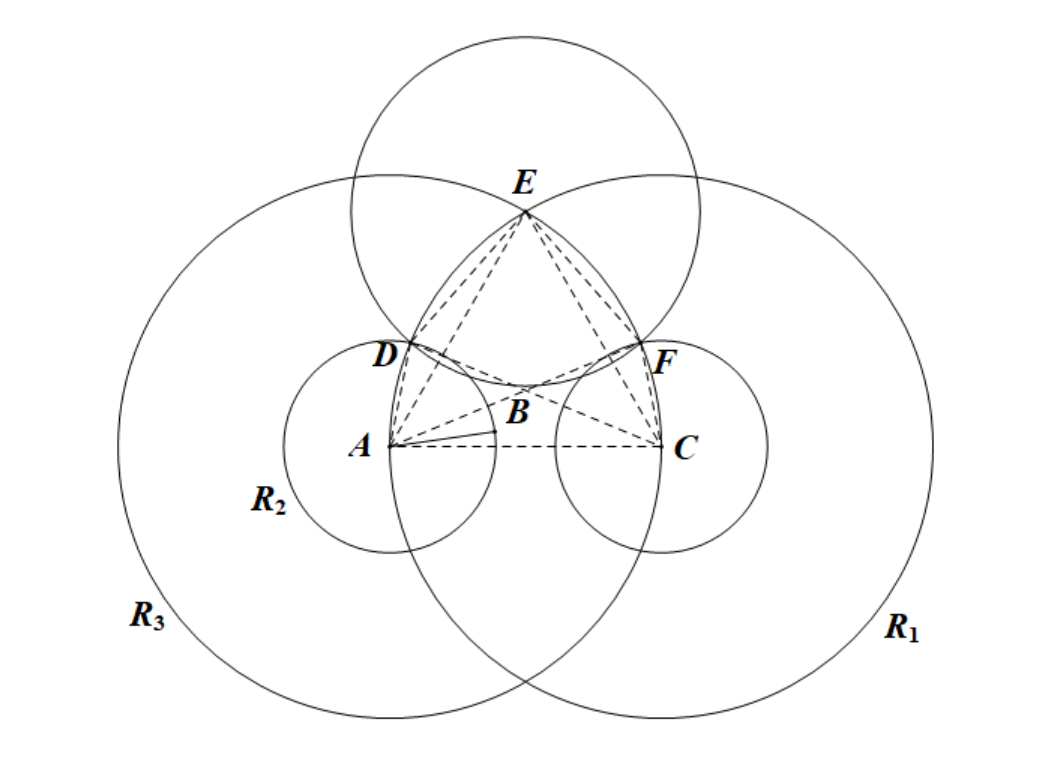
\includegraphics[width=10cm]{fig/plg_rc_compass.png}
\caption{以给定长度为半径作圆}
\label{fig:plg_rc_compass}
\end{figure}

上述命题表明尺规作图的作圆操作等价于“以已知点为圆心，两已知点距离为半径作圆”. 一种更为简明的作法是: 不妨设A、B、C三点不共线, 过C作AB平行线, 过B作AC平行线, 两直线交于点F, 则$CF=AB$. 


\begin{pro}\textbf{作线段中垂线}(步数3)
\par 如图\ref{fig:plg_rc_midpoint}, 给定线段AB, 以A为圆心、AB为半径作圆A，以B为圆心、AB为半径作圆B，两圆交于C、D，作直线CD交线段AB于M, 则$AM=BM$, 且$CD\perp AB$. 
\end{pro}
\begin{proof}
易得$\triangle ADC \cong \triangle BDC$, 故$\angle ACM = \angle BCM$. 又由$AC=BC$, $\triangle ACM \cong \triangle BCM$. 故$AM=BM$, $\angle AMC=\angle BMC=\frac{\pi}{2}$.
\end{proof}

\begin{pro}\textbf{作角平分线}(步数4)
\par 如图\ref{fig:plg_rc_bisectangle}, 以A为圆心的圆交角的两边于B, C；以B为圆心、BC为半径作圆，以C为圆心、BC为半径作圆，两圆交于D, 则$\angle BAD = \angle CAD$. 
\end{pro}

\begin{figure}[h]
\begin{minipage}{0.48\textwidth}
\centering
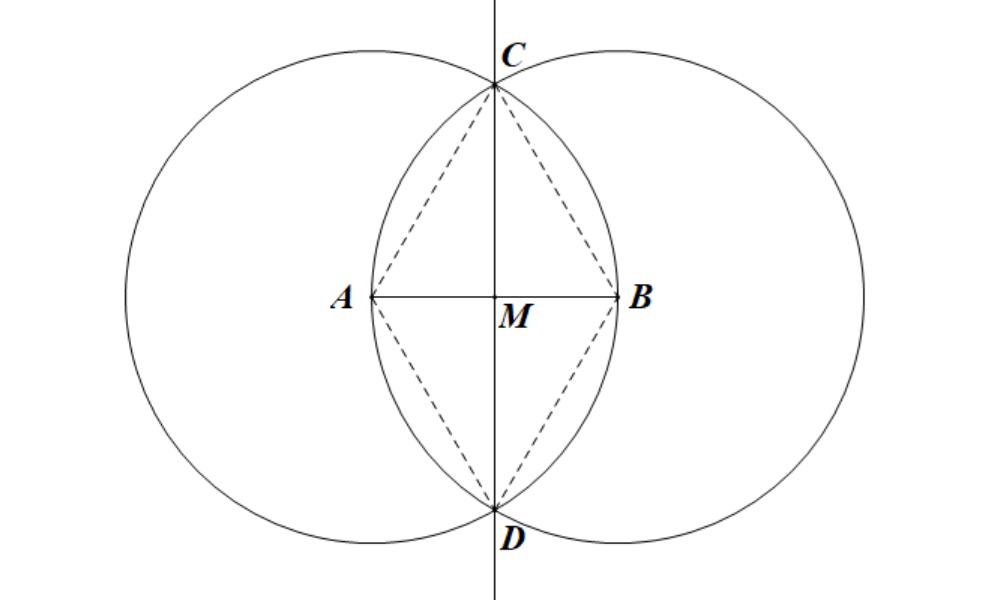
\includegraphics[width=7.5cm]{fig/plg_rc_midpoint.png}
\caption{尺规作线段中垂线}
\label{fig:plg_rc_midpoint}
\end{minipage}\hfill
\begin{minipage}{0.48\textwidth}
\centering
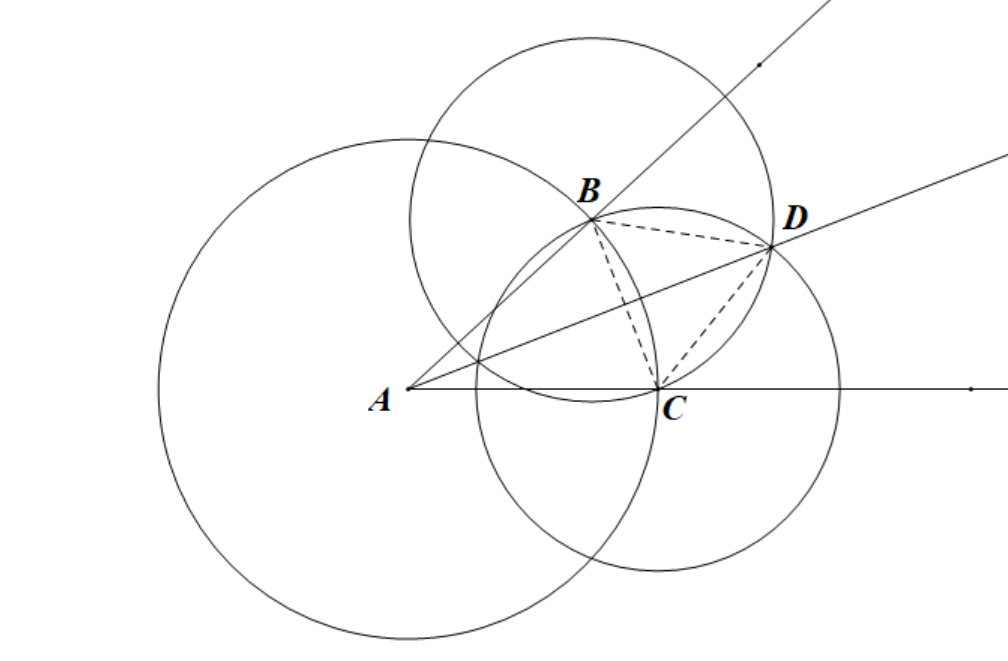
\includegraphics[width=7.5cm]{fig/plg_rc_bisectangle.png}
\caption{尺规作角平分线}
\label{fig:plg_rc_bisectangle}
\end{minipage}
\end{figure}


\begin{pro}\textbf{过直线外一点作垂线}(步数3)
\par 如图\ref{fig:plg_rc_perpendicular1}, 给定直线BC外一点A，以B为圆心、AB为半径作圆，以C为圆心、AB为半径作圆，两圆交于D, 则$AD \perp BC$. 
\end{pro}

\begin{pro}\textbf{过直线上一点作垂线}(步数3)
\par 如图\ref{fig:plg_rc_perpendicular2}, 给定直线上一点A，任取直线外一点O, 以O为圆心、OA为半径作圆，交直线于另一点B; 直线BO交圆O于点C, 则$CA \perp AB$. 
\end{pro}

\begin{figure}[h]
\begin{minipage}{0.48\textwidth}
\centering
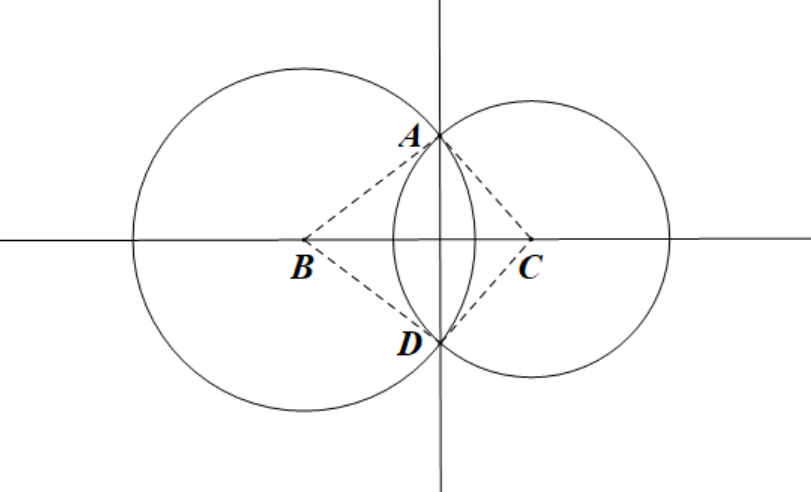
\includegraphics[width=8cm]{fig/plg_rc_perpendicular1.png}
\caption{尺规作过直线外一点的垂线}
\label{fig:plg_rc_perpendicular1}
\end{minipage}\hfill
\begin{minipage}{0.48\textwidth}
\centering
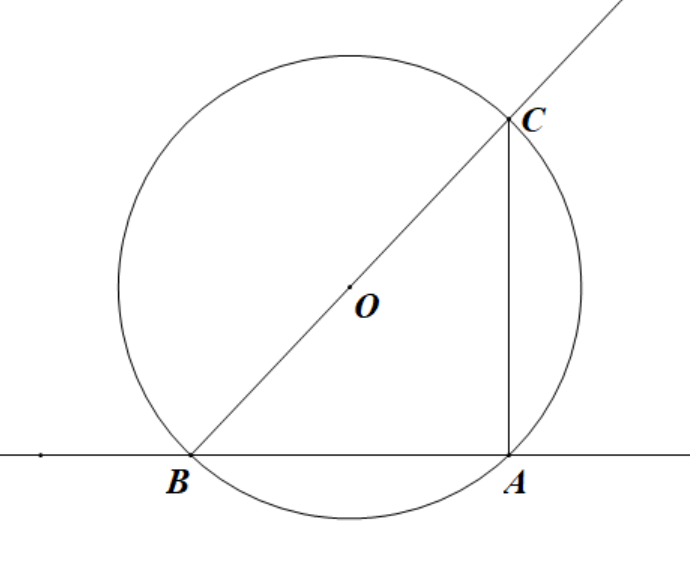
\includegraphics[width=6cm]{fig/plg_rc_perpendicular2.png}
\caption{尺规作过直线上一点的垂线}
\label{fig:plg_rc_perpendicular2}
\end{minipage}\hfill
\end{figure}

\begin{pro}\textbf{过直线外一点作平行线}(步数4)
\par 如图\ref{fig:plg_rc_parallel}, 给定直线AB外一点C，以A为圆心、AC为半径作圆，以B为圆心、BC为半径作圆，两圆交于C、D. 连接BD交圆B于点E, 则$CE \parallel AB$.  
\end{pro}

\begin{figure}[htb]
\centering
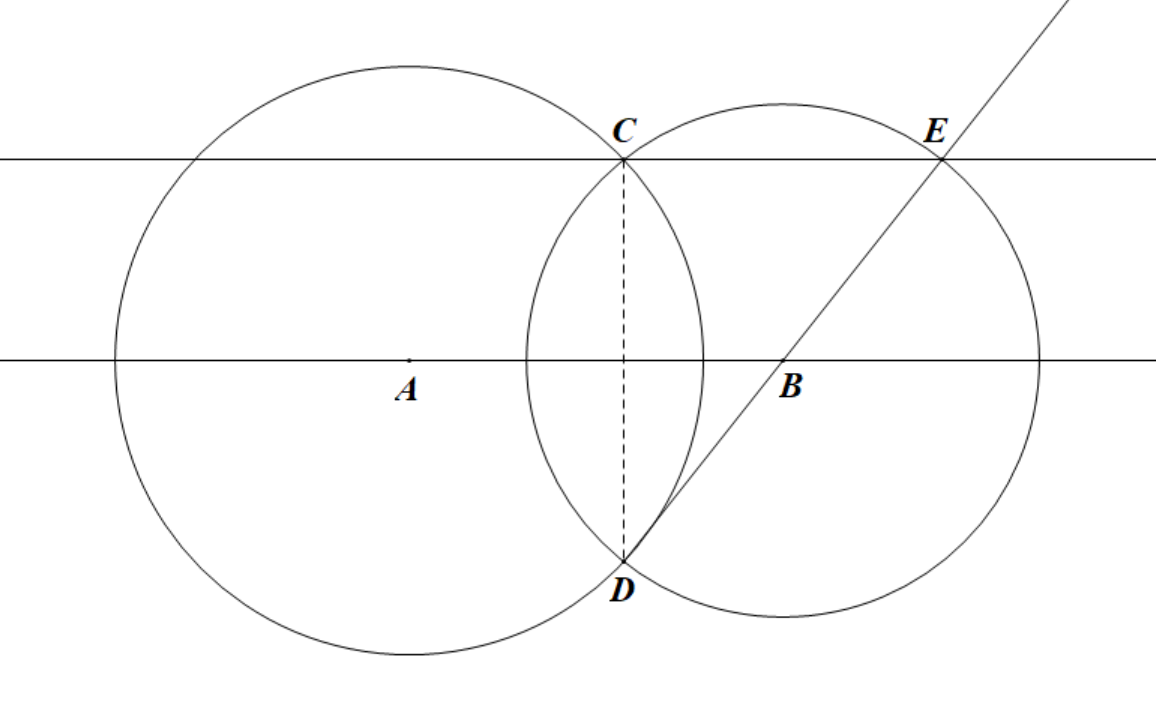
\includegraphics[width=8cm]{fig/plg_rc_parallel.png}
\caption{过直线外一点作平行线}
\label{fig:plg_rc_parallel}
\end{figure}

\section*{阅读材料}

互动游戏Euclidea\cite{Euclidea}包含大量尺规作图问题，许多问题最少步数的作法很具挑战性。

\section*{问题}
\newcounter{probplg} 

\stepcounter{probplg}
\par \textbf{\theprobplg .} \textbf{(作角等于已知角)} 给定$\angle A$和射线BC, 用尺规作$\angle DBC = \angle A$. 

\stepcounter{probplg}
\par \textbf{\theprobplg .} \textbf{(尺规作图的限度)} 设$z_1,z_2\in \mathbb{C}$, $r$是非负实数, 记$L(z_1,z_2)=\{z\in \mathbb{C}\vert \exists t\in \mathbb{R}: z=z_1+t(z_2-z_1)\}$; $C(z_1,r)=\{z\in \mathbb{C} : |z-z_1|=r\}$. 定义$\mathcal{P}_0=\{0,1\}$, $\mathcal{L}_0=\mathcal{C}_0=\varnothing$, 
\begin{align*}
\mathcal{L}_{n+1} & = \{L(z_1,z_2)\vert z_1, z_2\in \mathcal{P}_n \land z_1\neq z_2\}\\
\mathcal{C}_{n+1} & = \{C(z_1,|z_2-z_3|)\vert z_1, z_2, z_3\in \mathcal{P}_n \land  z_2\neq z_3\}\\
\mathcal{P}_{n+1} &  = \{z\in \mathbb{C} \vert \exists L_1,L_2\in \mathcal{L}_{n+1}: L_1 \neq L_2 \land z\in L_1\cap L_2\}\\
& \cup \{z\in \mathbb{C} \vert \exists C_1,C_2\in \mathcal{C}_{n+1}: C_1 \neq C_2 \land z\in C_1\cap C_2\} \\
&  \cup \{z\in \mathbb{C} \vert \exists C\in \mathcal{C}_{n+1} \exists L\in \mathcal{L}_{n+1}: z\in C\cap L\}
\end{align*}
并记$\mathcal{P}=\bigcup_{n\in \mathbb{N}} \mathcal{P}_{n}$. 

设$z\in \mathbb{C}$, 若存在$n\in\mathbb{N}$以及$\mathbb{C}$的子域$K_1,\dots,K_n$, 满足
\begin{equation*}
    \mathbb{Q}=K_0\subseteq K_1 \subseteq \cdots \subseteq K_n
\end{equation*}
$z\in K_n$, 且$[K_j:K_{j-1}]\le 2$对任意$j=1,\dots,n$成立, 称$z$为可构造数. 可构造数的集合记为$\mathbb{Q}^c$. 

设$\mathbb{C}$的子域$K$满足$z\in K \Rightarrow \exists r\in K: r^2=z$, 称$K$对开平方封闭. 

证明: 
(1) $\forall n\in \mathbb{N}$,  $\mathcal{P}_{n}$是有限集. 
(2) $\forall n\in \mathbb{N}$,  $\mathcal{P}_{n}\subseteq \mathcal{P}_{n+1}$. 
(3) $\forall n\in \mathbb{N}$, $z\in \mathcal{P}_n \Rightarrow \bar{z}\in \mathcal{P}_n$.
(4) $\mathbb{Q}^c$是$\mathbb{C}$的子域. 
(5) $z\in \mathbb{Q}^c \Rightarrow \bar{z} \in \mathbb{Q}^c$. 
(6) $\mathbb{Q}^c$对开平方封闭. 设$\mathbb{C}$的子域$K$对开平方封闭, 则$\mathbb{Q}^c \subseteq K$. 
(7) $z,w\in \mathcal{P} \Rightarrow z+w, -z, zw \in \mathcal{P}$; 当$z\neq 0$, 亦有$z^{-1}\in \mathcal{P}$. $\mathcal{P}$对开平方封闭.
(8) $\mathcal{P}=\mathbb{Q}^c$.
(9*) $\alpha\in \mathcal{P} \Rightarrow \exists k\in \mathbb{N}:[\mathbb{Q}(\alpha): \mathbb{Q}] = 2^k$. 举例说明逆命题不成立. 
(10) (\textbf{倍立方问题}) $\sqrt[3]{2}\notin \mathcal{P}$. 
(11) (\textbf{化圆为方问题}) $\sqrt{\pi}\notin \mathcal{P}$.
(12) (\textbf{三等分角问题}) $e^{\frac{2\pi \mathrm{i}}{3}}\in \mathcal{P}$, $e^{\frac{2\pi \mathrm{i}}{9}}\notin \mathcal{P}$.

\stepcounter{probplg}
\par \textbf{\theprobplg .} \textbf{(尺规作正多边形的可行性)}

(1*) 设$p$是素数, 则正$p$边形可用尺规作出当且仅当存在$k\in\mathbb{N}$, $p= 2^{2^k}+1$, 即$p$是Fermat素数. 

\stepcounter{probplg}
\par \textbf{\theprobplg .} \textbf{(有刻度直尺三等分角)} 如图\ref{fig:plg_trisect_angle}, 给定$\angle AOB$, 其中$A,B$位于以$O$为圆心、$r$为半径的圆上. 过$A$的直线交圆$O$于$D$, 交直线$BO$于$C$, 满足$CD=r$. 证明: $\angle ACB = \frac{1}{3} \angle AOB$. 

\begin{figure}[h]
\centering
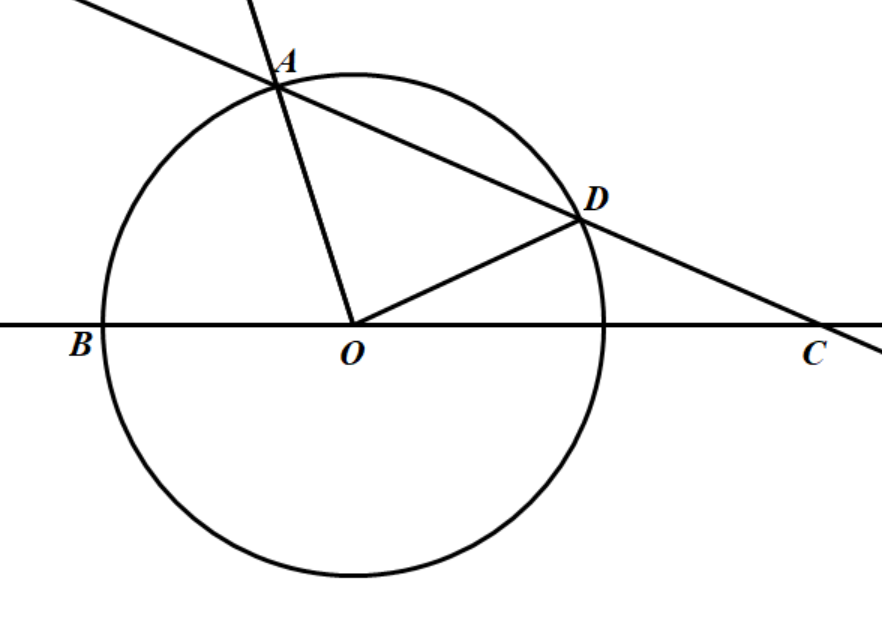
\includegraphics[width=6cm]{fig/plg_trisection_angle.png}
\caption{有刻度直尺三等分角}
\label{fig:plg_trisect_angle}
\end{figure}

\section*{解答}
\newcounter{solplg} 

\stepcounter{solplg}
\par \textbf{\thesolplg .} 如图\ref{fig:plg_copyangle}, 以任意长为半径作圆A交角的两边于E、F; 以B为圆心、AE为半径作圆交射线BC于G；以G为圆心、EF为半径作圆交圆B于D，则$\angle DBC = \angle A$. 

\begin{figure}[h]
\centering
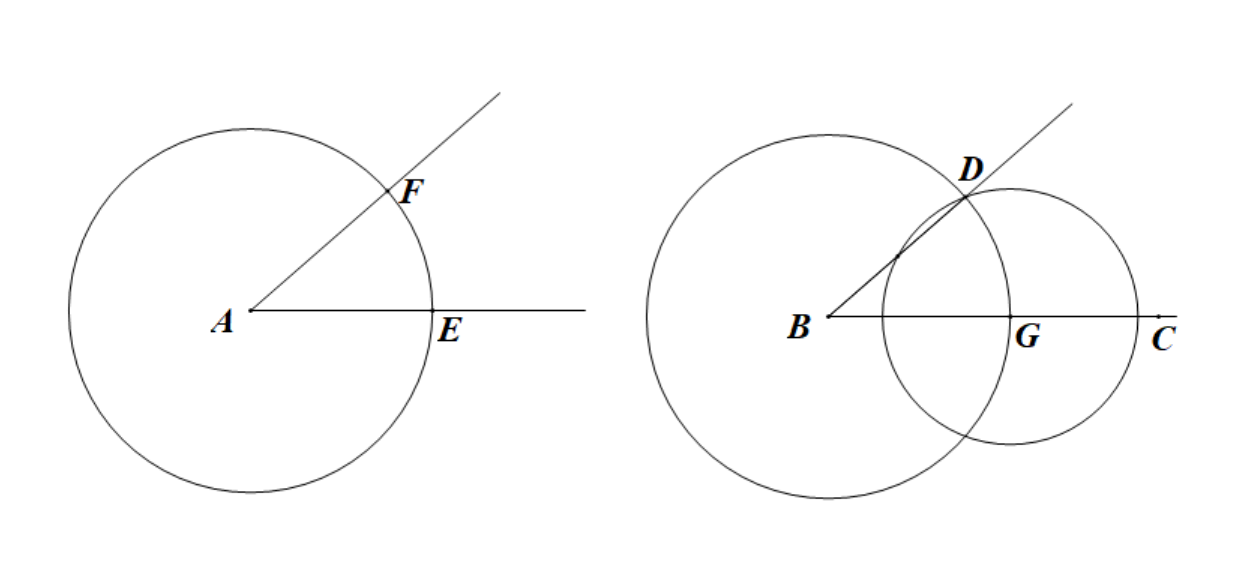
\includegraphics[width=9.6cm]{fig/plg_rc_copyangle.png}
\caption{作角等于已知角}
\label{fig:plg_copyangle}
\end{figure}

\stepcounter{solplg}
\par \textbf{\thesolplg .} (1) 对$n$归纳证明$\mathcal{L}_n$, $\mathcal{C}_n$, $\mathcal{P}_n$都是有限集. (2) 对$n$归纳证明$\mathcal{L}_n\subseteq \mathcal{L}_{n+1}$, $\mathcal{C}_n\subseteq \mathcal{C}_{n+1}$, $\mathcal{P}_n\subseteq \mathcal{P}_{n+1}$. 

(3) 对$n$归纳. $n=0$时显然成立. 设命题对$n-1$成立, 则$L(z_1,z_2)\in \mathcal{L}_n \Rightarrow L(\bar{z}_1,\bar{z}_2)\in \mathcal{L}_n$, $C(z_1,|z_2-z_3|)\in \mathcal{C}_n \Rightarrow C(\bar{z}_1,|\bar{z}_2-\bar{z}_3|)\in \mathcal{C}_n$. 当$z\in \mathcal{P}_n$, $z$为$\mathcal{P}_{n-1}$中特定点确定的$\mathcal{L}_n$中直线和/或$\mathcal{C}_n$中圆的交点，$\bar{z}$为其共轭点确定的$\mathcal{L}_n$中直线和/或$\mathcal{C}_n$中圆的交点，故$\bar{z}\in \mathcal{P}_n$. 

(4) 对$x,y\in \mathbb{Q}^c$, 设$\mathbb{C}$的子域$K_1,\dots,K_n$; $L_1,\dots, L_m$满足
\begin{align*}
\mathbb{Q}&=K_0 \subseteq K_1 \subseteq \cdots \subseteq K_n\\
\mathbb{Q}&=L_0 \subseteq L_1 \subseteq \cdots \subseteq L_m
\end{align*}
且$[K_i:K_{i-1}]=2$, $i=1,\dots,n$; $[L_j:L_{j-1}]=2$, $j=1,\dots,m$; $x\in K_n$, $y\in L_m$. 由素数次扩张是单扩张, 可设$K_i=K_{i-1}(\alpha_i)$, $i=1,\dots,n$; $L_j=L_{j-1}(\beta_j)$, $j=1,\dots,m$. 对$j=1,\dots,m$, 令$K_{n+j}=K_{n+j-1}(\beta_j)$, 则$x,y\in K_{n+m}$. 对$j=1,\dots,m$, 由于$\beta_j$在$L_{j-1}$上的极小多项式次数为2, 而$L_{j-1} \subseteq K_{n+j-1}$, 因此$\beta_j$在$K_{n+j-1}$上的极小多项式次数至多为2, $[K_{n+j},K_{n+j-1}]\le 2$. 因此$K_{n+m}$中的元素都是可构造数, 从而$x-y, xy$是可构造数; 当$y\neq 0$, $y^{-1}$也是可构造数. 命题得证. 

(5) 设$\mathbb{C}$的子域$K_1,\dots,K_n$满足$\mathbb{Q}=K_0 \subseteq K_1 \subseteq \cdots \subseteq K_n$, $z\in K_n$, 且$[K_i:K_{i-1}]=2$, $i=1,\dots,n$. 因此有$\mathbb{Q}=K_0 \subseteq \bar{K}_1 \subseteq \cdots \subseteq \bar{K}_n$, $\bar{z}\in \bar{K}_n$, 其中$\bar{K}_i = \{\bar{x} \vert x\in K_i\}$. 由$K_i$为$\mathbb{C}$的子域, $\bar{K}_i$也为$\mathbb{C}$的子域. 事实上, 设$x,y \in \bar{K}_i$, 则$\bar{x},\bar{y}\in K_i$, $\overline{x-y}=\bar{x}-\bar{y} \in K_i$, $\overline{xy}=\bar{x}\bar{y} \in K_i$; 从而$x-y, xy\in \bar{K}_i$. 当$y\neq 0$, $0 \neq \bar{y}\in K_i$, $\overline{y^{-1}}=(\bar{y})^{-1}\in K_i$, $y^{-1}\in \bar{K}_i$. 最后证明$[\bar{K}_i:\bar{K}_{i-1}]=[K_i:K_{i-1}]=2$. 事实上, 设$z_{i,1},z_{i,2}$是$K_{i-1}$上线性空间$K_i$的一个基, 则$\bar{z}_{i,1},\bar{z}_{i,2}$是$\bar{K}_{i-1}$上线性空间$\bar{K}_i$的一个基. 

(6) 设$z\in \mathbb{Q}^c$，则存在$\mathbb{C}$的子域$K_1,\dots,K_n$满足$\mathbb{Q}=K_0 \subseteq K_1 \subseteq \cdots \subseteq K_n$, $z\in K_n$, 且$[K_i:K_{i-1}]=2$, $i=1,\dots,n$. 设$r\in \mathbb{C}$是$x^2 - z$的一个零点, 令$K_{n+1}=K_n (r)$，则$[K_{n+1}: K_n] \le 2$, 故$r\in \mathbb{Q}^c$. 

设$\mathbb{C}$的子域$K$对开平方封闭, 对$n$归纳证明: 若$\mathbb{C}$的子域$K_1,\dots,K_n$满足$\mathbb{Q}=K_0 \subseteq K_1 \subseteq \cdots \subseteq K_n$, $z\in K_n$, 且$[K_i:K_{i-1}]=2$, $i=1,\dots,n$, 则$K_n \subseteq K$. 当$n=0$时, $\mathbb{Q}\subseteq K$显然成立. 设命题对$n-1$成立, 由素数次扩张是单扩张, 可设$K_n=K_{n-1}(\alpha)$. 设$\alpha$在$K_{n-1}$上的极小多项式为$x^2 + bx + c$, $b,c \in K_{n-1} \subseteq K$, 则由一元二次方程的求根公式及$K$对开平方封闭, 知$\alpha\in K$. 因此$K_n \subseteq K$. 得证.

(7) 命题即证明从给定复数出发, 由四则及开平方运算得到的复数对应的点可由尺规作出. 
\par (i) 设$\overrightarrow{OA}=z$， $\overrightarrow{OB}=w$, 当$O, A, B$不共线时，过A作OB的平行线，过B作OA的平行线，两直线交于$C$, 则$\overrightarrow{OC}=z+w$. 当$O, A, B$共线时，$C(z,|w|)$与$L(0,z)$的交点之一即为$z+w$. 
\par (ii) $C(0,|z|)$与$L(0,z)$的另一个交点即为$-z$. 
\par (iii) 为作$zw$, 只需作出角度$\arg z+\arg w$和长度$|z|\cdot |w|$. 前者只需以OA为一边向逆时针方向作角等于$\arg w$. 为作长度$|z|\cdot |w|$, 不妨设$z,w\neq 0$. 如图\ref{fig:plg_segmentmul}, 设$\overrightarrow{OA}=|z|$， $\overrightarrow{OB}=|w|$, $\overrightarrow{OC}=1$, 作$\overrightarrow{OD}=i$, $\overrightarrow{OE}=i|z|$, 过E作BD的平行线交OC于F, 则 $\overrightarrow{OF}=|z||w|$.

\begin{figure}[h]
\begin{minipage}{0.5\textwidth}
\centering
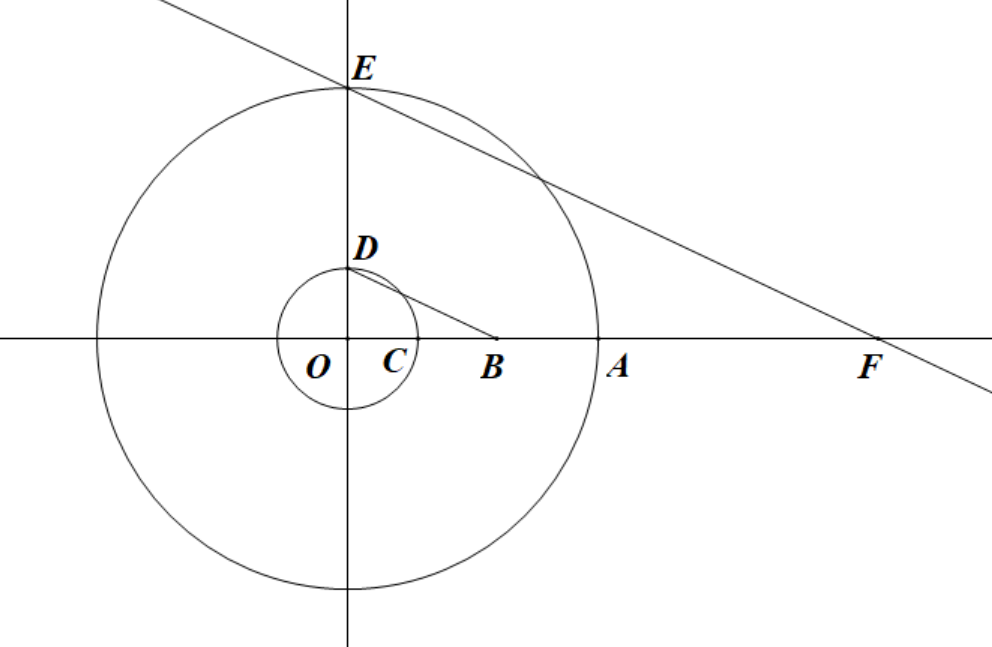
\includegraphics[width=7.2cm]{fig/plg_rc_segmentmul.png}
\caption{作线段长度乘积}
\label{fig:plg_segmentmul}
\end{minipage}\hfill
\begin{minipage}{0.5\textwidth}
\centering
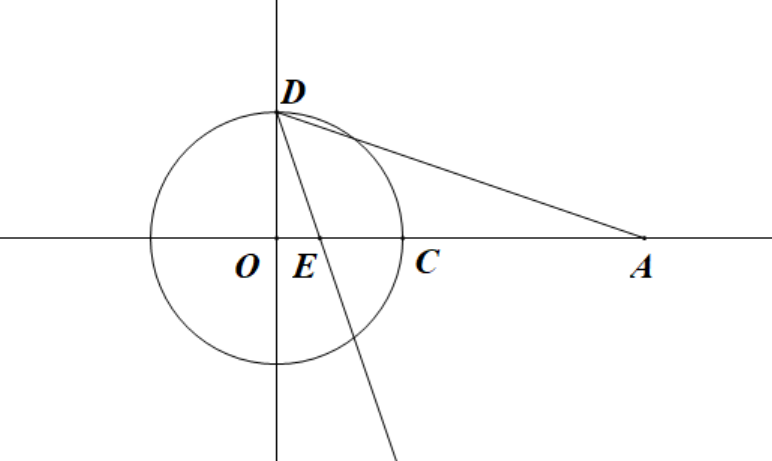
\includegraphics[width=7.2cm]{fig/plg_rc_segmentinv.png}
\caption{作线段长度倒数}
\label{fig:plg_segmentinv}
\end{minipage}\hfill
\end{figure}

\par (iv) 容易做出$\arg (z^{-1})=-\arg z$. 为作$|z^{-1}|=|z|^{-1}$, 设$\overrightarrow{OA} = |z|$, 如图\ref{fig:plg_segmentinv}, 设$\overrightarrow{OC}=1$, 作$\overrightarrow{OD}=i$, $\angle ODE = \angle OAD$, 则$OE = |z|^{-1}$. 

\par (v) 通过作角平分线容易做出$\arg \sqrt{z} = \frac{1}{2}\arg z$. 为作$|\sqrt{z}|=\sqrt{|z|}$, 不妨设$z\neq 0$, 如图\ref{fig:plg_segsqrt}, 设$\overrightarrow{OA}=|z|$, $\overrightarrow{OC}=1$, 容易作出$\overrightarrow{OD}=-1$. 作AD的中点E, $C(E, |DE|)$交纵轴于点F, 则$|OF|=\sqrt{|z|}$. 
由(ii)可作出$-\sqrt{z}$. 

\begin{figure}[h]
\centering
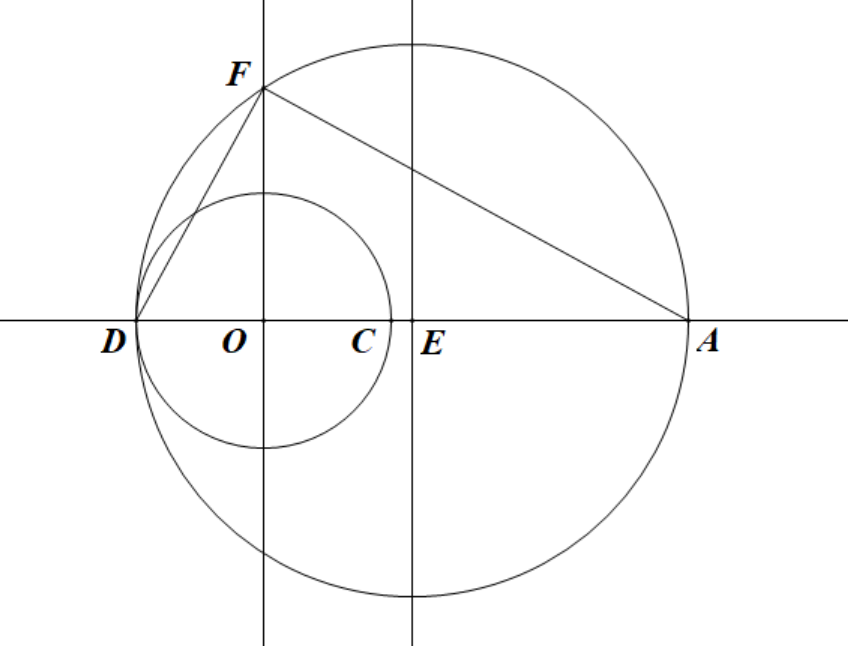
\includegraphics[width=8cm]{fig/plg_rc_segsqrt.png}
\caption{作线段长度平方根}
\label{fig:plg_segsqrt}
\end{figure}


(8) 先证$\mathcal{P} \subseteq \mathbb{Q}^c$. 对$n$归纳证明$\mathcal{P}_n \subseteq \mathbb{Q}^c$. $n=0$显然成立. 设命题对$n$成立, 考虑$n+1$的情形, 对$z\in \mathcal{P}_{n+1}$，分三种情况：(a) $z$是不同直线$L(z_1, z_2), L(z_3, z_4)$的交点, $z_1,z_2,z_3,z_4 \in \mathbb{Q}^c$. 由(5), 其共轭也属于$\mathbb{Q}^c$. 存在$a,b\in \mathbb{R}$, $z=az_1+(1-a)z_2=bz_3+(1-b)z_4$. 此时有
\begin{align*}
    (z_1-z_2)a+(z_4-z_3)b &= z_4-z_2\\
    (\bar{z}_1-\bar{z}_2)a+(\bar{z}_4-\bar{z}_3)b &= \bar{z}_4-\bar{z}_2
\end{align*}
上述关于$a,b$的线性方程组有唯一解，故$a$可由$z_1,z_2,z_3,z_4$及其共轭的加减乘除运算表出, $a\in \mathbb{Q}^c$, 从而$z\in \mathbb{Q}^c$. (b) $z$是直线$L(z_1, z_2)$与圆$C(z_3, |z_4-z_5|)$的交点, $z_1,z_2,z_3, z_4, z_5 \in \mathbb{Q}^c$. 令$r=|z_4-z_5|$, 则存在$a, \theta\in \mathbb{R}$, $z=az_1+(1-a)z_2=z_3+re^{\mathrm{i}\theta}$. 
此时有
\begin{align*}
    (z_1-z_2)a+z_2-z_3 &= re^{\mathrm{i}\theta}\\
    (\bar{z}_1-\bar{z}_2)a+\bar{z}_2-\bar{z}_3 &= re^{-\mathrm{i}\theta}
\end{align*}
两式相乘得
\begin{equation*}
    (a(z_1-z_2)+z_2-z_3)(a(\bar{z}_1-\bar{z}_2)+\bar{z}_2-\bar{z}_3) = r^2=(z_4-z_5)(\bar{z}_4-\bar{z}_5)
\end{equation*}
此为关于$a$的二次方程, 其系数均在$\mathbb{Q}^c$中. 由$\mathbb{Q}^c$对开平方封闭, $a\in \mathbb{Q}^c$, 从而$z\in \mathbb{Q}^c$. (c) $z$是不同圆$C(z_1, |z_2-z_3|)$与$C(z_4, |z_5-z_6|)$的交点, $z_1,z_2,z_3, z_4, z_5, z_6 \in \mathbb{Q}^c$. 令$r=|z_2-z_3|$, $s=|z_5-z_6|$, 则存在$\theta, \phi\in \mathbb{R}$, $z=z_1+re^{\mathrm{i}\theta}=z_4+se^{\mathrm{i}\phi}$.  
此时有
\begin{align*}
    (z-z_1)(\bar{z}-\bar{z}_1)&= r^2\\
    (z-z_4)(\bar{z}-\bar{z}_4)&= s^2
\end{align*}
消去$\bar{z}$得到关于$z$的二次方程, 其系数均在$\mathbb{Q}^c$中, 故$z\in \mathbb{Q}^c$.

\par 再证$\mathbb{Q}^c \subseteq \mathcal{P}$. 对$n$归纳证明: 若$\mathbb{C}$的子域$K_1,\dots,K_n$满足$\mathbb{Q}=K_0 \subseteq K_1 \subseteq \cdots \subseteq K_n$, 且$[K_i:K_{i-1}]=2$, $i=1,\dots,n$, 则$K_n \subseteq \mathcal{P}$. 由(7), 任意$q\in \mathbb{Q}$可由$0,1$出发用尺规作出, 从而$\mathbb{Q}\subseteq \mathcal{P}$, $n=0$成立. 设命题对$n$成立, 则由$[K_{n+1}:K_n]=2$知存在$\alpha\in K_{n+1}$, $K_{n+1} = K_n(\alpha)$, 且$\alpha$的极小多项式次数为2. 由二次方程求根公式, $\alpha$可由$K_n$中的数经过四则运算及开平方得到, 由$K_n \subseteq \mathcal{P}$及(7), $\alpha\in \mathcal{P}$, 从而$K_{n+1}\subseteq \mathcal{P}$. 得证. 

\emph{注}: 尺规作图的给定点可推广到有限集$P\subseteq \mathbb{C}$, 满足$\{0,1\} \subseteq P$, 且$z\in P\Rightarrow \bar{z} \in P$. 此时改为$\mathcal{P}_0=P$, 同理可证复数$z$可用尺规作出的充要条件为: 存在$n\in \mathbb{N}$及$\mathbb{C}$的子域$K_1,\dots,K_n$, 满足$\mathbb{Q}(P) = K_0 \subseteq K_1 \subseteq \cdots \subseteq K_n$, $z\in K_n$, $[K_j:K_{j-1}]\le 2$对任意$j=1,\dots,n$成立. 

(9) 由(8)及域扩张次数的性质即得. 

(10) 由Eisenstein判别法, $x^3-2$在$\mathbb{Q}[x]$上不可约, 因此$x^3-2$是$\sqrt[3]{2}$在$\mathbb{Q}$上的极小多项式, $[\mathbb{Q}(\sqrt[3]{2}): \mathbb{Q}]=3$. 

(11) 若$\sqrt{\pi}\in \mathcal{P}$, 则$\pi \in \mathcal{P}$. 但由Lindemann定理, $\pi$是$\mathbb{Q}$上的超越元, $[\mathbb{Q}(\pi):\mathbb{Q}]$无限, 矛盾. 

(12) 设$\zeta=e^{\frac{2\pi i}{9}}\in \mathcal{P}$, 则$\alpha = \zeta + \zeta^{-1} \in \mathcal{P}$. 而$\alpha^3 = \zeta^6 + \zeta^3 + 3\zeta + 3\zeta^{-1} = -1 + 3\alpha$, 因此$\alpha$是$x^3-3x+1$的一个零点. 容易验证$x^3-3x+1$在$\mathbb{Z}[x]$上不可约（$|x||x^2-3|=1$没有整数解），由Gauss引理，其在$\mathbb{Q}[x]$上也不可约, 从而是$\alpha$的极小多项式, $[\mathbb{Q}(\alpha):\mathbb{Q}]=3$, 矛盾. 

\stepcounter{solplg}
\par \textbf{\thesolplg .} 正$p$边形的外角为$\frac{2\pi}{p}$. 因此正$p$边形可用尺规作出等价于$\zeta_p=e^{\frac{2\pi i}{p}}$是可构造数. 必要性: $e^{\frac{2\pi i}{p}}$是$\Phi_p(z)=\frac{z^{p}-1}{z-1}=1+z+\cdots z^{p-1}$的一个零点. 当$p$为素数时, $\Phi_p(z)$在$\mathbb{Q}[x]$上不可约, 从而是$\zeta_p$在$\mathbb{Q}$上的极小多项式. 因此$[\mathbb{Q}(\zeta_p):\mathbb{Q}]=p-1$, 故存在正整数$m$, $p=2^m+1$. 若$m$包含奇素因子$b$, 设$m=ab$, 则$2^a+1\vert 2^{ab}+1$, 与$p$是素数矛盾. 故$m$只能为2的非负整数次幂, 即$p$是Fermat素数. 

\stepcounter{solplg}
\par \textbf{\thesolplg .} $\angle AOB=\angle OAD +\angle ACB$. 由$OA=OD=CD$, $\angle OAD = \angle ODA = 2\angle ACB$.  

\chapter{立体几何}

\chapter{球面几何}

\chapter{圆锥曲线与二次曲面}

\chapter{微分几何}

\chapter{代数几何}

\part{概率}
\chapter{概率}


\begin{dfn}\textbf{概率空间} Probability Space\\
三元组$(\Omega, F, P)$称为概率空间, 其中:
\begin{itemize}
\item 全集$\Omega$是非空集合.
\item $F\subseteq \mathcal{P} (\Omega)$满足: (1) $\Omega \in F$; (2) $A\in F \Rightarrow A' \in F$; (3) 若对任意正整数$i$, $A_i \in F$, 则$ \bigcup_{i=1}^\infty A_i \in F$. 
\item 函数$P: F\to [0,1]$满足: (1) $P(\Omega)=1$; (2) 若$A_1,A_2,\dots,A_n,\dots \in F$两两不相交, 则
\begin{equation}
    P\left(\bigcup_{i=1}^\infty A_i \right)=\sum_{i=1}^\infty P(A_i)
\end{equation}
\end{itemize}
称$\Omega$为样本空间; $F$为$\Omega$的事件域, $F$中的元素为事件; $P$为$F$上的概率测度. 
\end{dfn}

\begin{pro}\textbf{概率测度的性质}\\
设$(\Omega, F, P)$为概率空间, $A\in F$,
\begin{enumerate}
\item $P(A')=1-P(A)$;
\item $P(\varnothing)=0$.
\end{enumerate}
\end{pro}

\section*{文献注记}

\section*{问题}
\newcounter{probprob} 
\stepcounter{probprob}
\par \textbf{\theprobprob .} (\textbf{奖券收集问题}) 设随机变量$\{X_n\}_{n\in \mathbb{N}}$相互独立, 均服从$\{1,2,\dots,k\}$上的均匀分布. 令
\begin{align}
    C_n &= \{X_1,\dots,X_n\} \\
    T &= \inf \{n\in \mathbb{N}: |C_n| = k\}
\end{align}
证明: (1) $E T = kH_k$, 其中$H_k=\sum_{i=1}^k \frac{1}{i}$. (2) $P(T=n)=\frac{k!S(n-1,k-1)}{k^n}$, 其中$S(n-1,k-1)$是第二类Stirling数. 

\section*{解答}
\newcounter{solprob} 
\stepcounter{solprob}
\par \textbf{\thesolprob .} (1) \cite{MaP} 对$l=1,2,\dots,k$, 记$T_l = \inf \{n\in \mathbb{N}: |C_n| = l\} - \inf \{n\in \mathbb{N}: |C_n| = l-1\}$, 则$T_1=1$, $T=\sum_{l=1}^k T_l$. $T_l$服从成功概率为$\frac{k-l+1}{k}$的几何分布:
\begin{equation}
    P(T_l=i)=\left(1-\frac{l-1}{k}\right)^{i-1} \frac{k-l+1}{k}
\end{equation}
故有
\begin{equation}
    ET=\sum_{l=1}^k ET_l = \sum_{l=1}^k \frac{k}{k-l+1} = kH_k
\end{equation}
(2) 序列$(X_1,\dots,X_n)$有$k^n$种. 为满足$T=n$, $|C_{n-1}|=k-1$且$X_n = \{1,\dots,k\} - C_{n-1}$. $X_n$有$k$种取法, 对给定$X_n$, $(X_1,\dots,X_{n-1})$的取法等于$\{1,2,\dots,n-1\}$到$\{1,\dots,k\}-\{X_n\}$的满射数, 即为$(k-1)! S(n-1,k-1)$. 命题得证. 
\chapter{随机过程}

\part{组合}
\chapter{计数组合学}

\par 计数组合学(enumerative combinatorics)的基本问题是计算有限集合的元素个数（一种常见情形是以自然数为指标集的一族集合）. 计数的结果可以是：(1)显式的闭公式（不含求和号，仅含常见函数）；(2)递推式；(3)算法；(4)渐近估计$f(n)\sim g(n)$，即$\lim \limits_{n\to \infty} \frac{f(n)}{g(n)}=1$；(5)生成函数(generating function). 

\section{二项式系数}

\begin{dfn} \textbf{二项式系数}\\
设$\lambda \in \mathbb{C}$，$k \in \mathbb{N}$，定义
\begin{equation}
    \binom{\lambda}{k}=\frac{\lambda(\lambda-1)\cdots (\lambda-k+1)}{k!}
\end{equation}
\end{dfn}
特别地, 当$n\in \mathbb{N}$, 且$k
\le n$, 有
\begin{equation}
    \binom{n}{k}=\frac{n!}{k!(n-k)!}
\end{equation}
当$k>n$, 有$\binom{n}{k}=0$. 有时也将$\lambda(\lambda-1)\cdots (\lambda-k+1)$记作$[\lambda]_k$, 从而$\binom{\lambda}{k}=[\lambda]_k/k!$. 

\begin{pro} \textbf{二项式系数相关恒等式}\\
设$\lambda \in \mathbb{C}$, $n, k\in \mathbb{N}$, $0\le k\le n$, 
\begin{enumerate}
\item $\displaystyle \binom{n}{k}=\binom{n}{n-k}$.
\item $\displaystyle \binom{\lambda}{k}+\binom{\lambda}{k+1}=\binom{\lambda+1}{k+1}$.
\item $\displaystyle \sum_{i=0}^{k} \binom{\lambda+i}{i}=\binom{\lambda+k+1}{k}$. 
\item 当$k\ge 1$, $\displaystyle k\binom{\lambda}{k}=\lambda\binom{\lambda-1}{k-1}$. 

\end{enumerate}
\end{pro}
\begin{proof} (1)显然. (2) 
\begin{align}
    \binom{\lambda}{k}+\binom{\lambda}{k+1}&=\frac{\lambda (\lambda-1)\cdots (\lambda-k+1)}{k!}+\frac{\lambda (\lambda-1)\cdots (\lambda-k)}{(k+1)!}\notag\\
    &=(k+1+\lambda-k)\frac{\lambda (\lambda-1)\cdots (\lambda-k+1)}{(k+1)!}=\binom{\lambda+1}{k+1}
\end{align}
(3) 注意到$\binom{\lambda}{0}=\binom{\lambda+1}{0}=1$, 对等式左边重复使用(2)即证. (4) 当$k\ge 1$时,
\begin{equation}
k\binom{\lambda}{k} = \frac{\lambda (\lambda-1)\cdots (\lambda-k+1)}{(k-1)!} = \lambda\binom{\lambda-1}{k-1}
\end{equation}
\end{proof}

\par (3)的一个特例是$\displaystyle \sum_{i=0}^{n-k} \binom{k+i}{k} = \binom{n+1}{k+1}$. 

\begin{pro} \textbf{二项式系数的单峰性}\\
设$n\in \mathbb{N}$, 则
\begin{equation}
    \max_{0\le k\le n} \binom{n}{k} = \binom{n}{\lfloor \frac{n}{2}\rfloor} = \binom{n}{\lceil \frac{n}{2}\rceil}
\end{equation}
且当$0\le k< \lfloor \frac{n}{2}\rfloor$时, $\displaystyle \binom{n}{k} < \binom{n}{k+1}$; 当$\lceil \frac{n}{2}\rceil \le k < n$时, $\displaystyle \binom{n}{k} > \binom{n}{k+1}$. 
\end{pro}
\begin{proof} 设$0\le k<n$, 
\begin{equation}
    \binom{n}{k}/\binom{n}{k+1} = \frac{k+1}{n-k}
\end{equation}
故$\displaystyle \binom{n}{k} < \binom{n}{k+1} \iff k<\frac{n-1}{2} \iff k< \left\lfloor \frac{n}{2}\right\rfloor$. 
\end{proof}

\begin{thm}\textbf{二项式定理} Binomial Theorem\\
设$x,y\in \mathbb{C}$, $n\in \mathbb{N}$, 
\begin{equation}
    (x+y)^n = \sum_{k=0}^n \binom{n}{k} x^{n-k}y^k
\end{equation}
\label{thm:binomial}
\end{thm}
\begin{proof}
对$n$用数学归纳法, $n=0$显然. 设命题对$n$成立, 则
\begin{align*}
    (x+y)^{n+1} &= (x+y)^n(x+y)\\
    &= \sum_{k=0}^n \binom{n}{k} x^{n+1-k}y^k + \sum_{k=0}^{n} \binom{n}{k} x^{n-k}y^{k+1}\\
    &= \sum_{k=0}^n \binom{n}{k} x^{n+1-k}y^k + \sum_{k=1}^{n+1} \binom{n}{k-1} x^{n+1-k}y^{k}\\
    &= \sum_{k=0}^{n+1} \binom{n+1}{k}x^{n+1-k}y^k
\end{align*}
\end{proof}

\begin{col}\textbf{二项式系数求和}\\
设$n$为正整数, 
\begin{align}
    &\sum_{k=0}^n \binom{n}{k}=2^n\\
    &\sum_{k=0}^n (-1)^k \binom{n}{k}=0
\end{align}
\end{col}
\begin{proof}
在定理\ref{thm:binomial}中分别令$x=y=1$; $x=1, y=-1$即得. 
\end{proof}
以上两式的组合含义为: 设$|X|=n$, $X$的子集个数$|\mathcal{P}(X)|=2^n$等于$0,1,\dots,n$元子集个数之和 (命题\ref{pro:setsize}, 推论\ref{col:setsize}); 奇数个元素的子集个数等于偶数个元素的子集个数(均为$2^{n-1}$). 

\begin{pro}\textbf{Vandermonde卷积公式} Vandermonde convolution\\
设$m_1,m_2,n$为正整数, 
\begin{equation}
    \sum_{k=0}^n \binom{m_1}{k} \binom{m_2}{n-k} = \binom{m_1+m_2}{n}
\end{equation}
\end{pro}
\begin{proof}
考虑$(1+x)^{m_1}(1+x)^{m_2}=(1+x)^{m_1+m_2}$中$x^n$项的系数. 
\end{proof}

\begin{dfn} \textbf{多项式系数}\index{多项式系数}\\
设$n$为正整数，自然数$n_1,\dots,n_k$和为$n$，定义
\begin{equation}
    \binom{n}{n_1\;\cdots\;n_k}=\frac{n!}{n_1!\cdots n_k!}
\end{equation}
\end{dfn}

\begin{thm}\textbf{多项式定理} Multinomial Theorem\\
设$x_1,\dots,x_k \in \mathbb{C}$, $n\in \mathbb{N}$, 
\begin{equation}
    (x_1+\dots+x_k)^n = \sum_{\substack{(n_1,\dots,n_k)\\n_1+\dots +n_k=n}} \binom{n}{n_1\;\cdots\;n_k} x_1^{n_1}\cdots x_k^{n_k}
\end{equation}
\label{thm:multinomial}
\end{thm}
\begin{proof}
考虑$x_1^{n_1}\cdots x_k^{n_k}$项, 设从第$j$个因式$(x_1+\dots+x_k)$中选取的项为$x_{r_j}$, $j=1,\dots,k$, 则$(r_1,\dots,r_n)$是$n_1$个$x_1$, $n_2$个$x_2$, $\dots$, $n_k$个$x_k$的一个可重复排列. 由命题\ref{pro:repeat_permutation}, 这样的可重复排列的个数为$\binom{n}{n_1\;\cdots\;n_k}$. 
\end{proof}

\section{生成函数}

\begin{dfn} \textbf{一般、指数生成函数}\index{一般生成函数}\index{指数生成函数}\\
设$f: \mathbb{N} \to \mathbb{C}$， $f$的一般生成函数为形式幂级数
\begin{equation*}
    \sum_{n=0}^\infty f(n)x^n
\end{equation*}
$f$的指数生成函数为形式幂级数
\begin{equation*}
    \sum_{n=0}^\infty \frac{f(n)}{n!}x^n
\end{equation*}
\end{dfn}

\par 生成函数可按照$\mathbb{C}[[x]]$中的运算进行加法、乘法运算；当常数项非0时，可以进行求逆运算。

\begin{dfn} 
\textbf{形式幂级数的收敛}\\
设$\{F_i(x)\}_{i=1}^\infty$是$ \mathbb{C}[[x]]$中的形式幂级数序列， 若存在$F(x)=\sum_{n\ge0} a_nx^n \in \mathbb{C}[[x]]$，对任意整数$n \ge 0$，存在正整数$\delta_n$，当$i>\delta_n$时$F_i(x)$中$x^n$的系数都为$a_n$，则称$F_i(x)$收敛于$F(x)$，记作$F_i(x) \to F(x)$。
\end{dfn}

\begin{pro}
\textbf{形式幂级数收敛的等价定义}\\
形式幂级数序列$F_i(x)$收敛等价于
\begin{equation}
    \lim \limits_{i\to \infty} \deg(F_{i+1}(x)-F_{i}(x))=\infty
\end{equation}
\end{pro}

\begin{dfn} 
\textbf{形式幂级数无穷级数的值}\\
若$\sum_{i=0}^j F_i(x)\to F(x)$，称无穷级数$\sum_{i=0}^\infty F_i(x)$的值为$F(x)$。
\end{dfn}

\begin{col}
\textbf{形式幂级数无穷级数收敛的充要条件}\\
无穷级数$\sum_{i=0}^\infty F_i(x)$收敛当且仅当
\begin{equation}
    \lim \limits_{i\to \infty} \deg F_{i}(x)=\infty
\end{equation}
\label{ser_cov}
\end{col}

\begin{dfn} 
\textbf{形式幂级数无穷乘积的值}\\
若$F_i(0)=1$对任何$i\ge 1$成立，$\prod_{i=1}^j F_i(x)\to F(x)$，称无穷乘积$\prod_{i=1}^\infty F_i(x)$的值为$F(x)$。
\end{dfn}

\begin{col}
\textbf{形式幂级数无穷乘积收敛的充要条件}\\
若$G_i(0)=0$对任何$i\ge 1$成立，无穷乘积$\prod_{i=1}^\infty (1+G_i(x))$收敛当且仅当
\begin{equation}
    \lim \limits_{i\to \infty} \deg G_{i}(x)=\infty
\end{equation}
\end{col}
\begin{proof}
只需注意到
\begin{align*}
    \deg \left(\prod_{i=1}^{j+1}(1+G_i(x))-\prod_{i=1}^{j}(1+G_i(x))\right)&=\deg\left(G_{j+1}(x)\prod_{i=1}^{j}(1+G_i(x))\right)\\
    &=\deg G_{j+1}(x)
\end{align*}
\end{proof}

\par 对于收敛的级数和无穷乘积，给定$n$，$x^n$的系数可通过有限步运算得到。

\begin{dfn} 
\textbf{形式幂级数的复合}\\
若形式幂级数$F(x)=\sum_{n\ge 0} a_nx^n$，$G(0)=0$；则复合幂级数$F(G(x))$定义为$\sum_{n\ge 0} a_nG(x)^n$.
\end{dfn}
根据推论\ref{ser_cov}，上述定义的复合幂级数收敛。

\begin{dfn} 
\textbf{形式幂级数的形式微分}\\
形式幂级数$F(x)=\sum_{n\ge 0} a_nx^n$的形式微分定义为
\begin{equation}
    F'(x)=\sum_{n\ge 1} na_nx^{n-1}=\sum_{n\ge 0} (n+1)a_{n+1}x^n
\end{equation}
\end{dfn}

\begin{pro}
\textbf{形式幂级数的形式微分公式}\\
函数和、积、复合的微分公式对形式幂级数仍成立。
\begin{align}
    (F+G)' &= F'+G'\\
    (FG)' &= F'G +FG'\\
    (F^n)' &= nF^{n-1}F'\\
    F(G(x))'&= G'(x)F'(G(x))
\end{align}
\end{pro}

\section{计数序列}
\begin{dfn} \textbf{Catalan数}\\
Catalan数$C_n$满足$C_0=1$; 对$n\ge 1$, 
\begin{equation}
    C_n = \sum_{k=0}^{n-1} C_kC_{n-1-k}
\end{equation}
\end{dfn}

\begin{pro}\textbf{Catalan数的通项公式}\\
\begin{equation}
    C_n = \frac{1}{n+1}\binom{2n}{n}
\end{equation}
\end{pro}
\begin{proof}
记$C_{n}$的一般生成函数为$g(x)$, 则有
\begin{equation}
    xg(x)^2 = x\left(\sum_{n=1}^\infty C_{n-1}x^n\right)^2 = \sum_{n=0}^\infty \left(\sum_{k=0}^{n} C_kC_{n-k}\right) x^{n+1}=g(x)-1
\end{equation}
因此$g(x)=\frac{1\pm \sqrt{1-4x}}{2x}$. 又由于$\lim\limits_{x\to 0} g(x) = 1$, 根号前只能取负号. 幂级数展开得
\begin{align*}
g(x)&=\frac{1}{2x}(1-\sqrt{1-4x})= \frac{1}{2x}\sum_{n=1}^\infty \frac{2}{n}\binom{2n-2}{n-1}x^n\\
&= \sum_{n=1}^\infty \frac{1}{n}\binom{2n-2}{n-1}x^{n-1} = \sum_{n=0}^\infty \frac{1}{n+1}\binom{2n}{n}x^{n}
\end{align*}
\end{proof}

Catalan数的前几项是$C_0=C_1=1$, $C_2=2$, $C_3=5$, $C_4=14$, $\cdot$.  

\begin{dfn} \textbf{第一类Stirling数}\\
第一类Stirling数$s(n,k)$满足$s(0,0)=1$; $k\ge 1$时$s(0,k)=0$; $n\ge 1$时$s(n,0)=0$. 当$n,k\ge 1$, 
\begin{equation}
    s(n,k)=(n-1)s(n-1,k)+s(n-1,k-1)
\end{equation}
\end{dfn}
当$n\ge 1$时, 对$n$归纳可证明$s(n,n)=1$, $k>n$时$s(n,k)=0$; $s(n,1)=(n-1)!$; $s(n,n-1)=\frac{n(n-1)}{2}$.

\begin{dfn} \textbf{第二类Stirling数}\\
第二类Stirling数$S(n,k)$满足$S(0,0)=1$; $k\ge 1$时$S(0,k)=0$; $n\ge 1$时$S(n,0)=0$. 当$n,k\ge 1$, 
\begin{equation}
    S(n,k)=kS(n-1,k)+S(n-1,k-1)
\end{equation}
\end{dfn}
当$n\ge 1$时, 对$n$归纳可证明 $S(n,n)=1$, $k>n$时$S(n,k)=0$; $S(n,1)=1$; $S(n,2)=2^{n-1}-1$; $S(n,n-1)=\binom{n}{2}$.

\begin{pro}\textbf{第二类Stirling数的通项公式}\\
\begin{equation}
    S(n,k)=\frac{1}{k!} \sum_{t=0}^k (-1)^t \binom{k}{t} (k-t)^n
\end{equation}
\end{pro}

\begin{proof}
设$X$, $Y$是有限集, $|X|=n$, $Y=\{y_1,\dots.y_k\}$, 对映射$f:X\to Y$中的满射进行计数. 定义条件$P_i(f): y_i \notin f(X)$, $i=1,\dots,k$, 则由容斥原理, 不满足任一$P_i$的映射数为
\begin{equation*}
    \sum_{t=0}^k (-1)^t \binom{k}{t} (k-t)^n
\end{equation*}
由命题\ref{pro:12fold-1} 即得证.  
\end{proof}

\begin{dfn} \textbf{Bell数}\\
Bell数$B_n$满足
\begin{equation}
    B_n=\sum_{k=0}^n S(n,k)
\end{equation}
其中$S(n,k)$是第二类Stirling数. 
\end{dfn}
Bell数的前几项是$B_0=1$, $B_1=1$, $B_2=2$, $B_3=5$, $B_4=15$, $\cdots$. 


\begin{dfn} \textbf{Bernoulli数}\\
Bernoulli数$B_n$满足$B_0=1$, 
\begin{equation}
    B_n =-\sum_{k=0}^{n-1}\binom{n}{k}\frac{B_k}{n-k+1}
\end{equation}
\end{dfn}
\par Bernoulli数的前几项是$B_0=1$, $B_1=-\frac{1}{2}$, $B_2=\frac{1}{6}$, $B_3=0$, $B_4=-\frac{1}{30}$, $\cdots$. 

\section{计数方法}

\subsection{基本计数公式}

\begin{pro} \textbf{鸽巢原理} Pigeonhole Principle \\
设非空有限集$|X|=n$, $|Y|=m$, 函数$f:X\to Y$, 则存在$y\in Y$, $|f^{-1}(y)|\ge \lceil\frac{n}{m}\rceil$. 
\end{pro}
\begin{proof}
反设$\forall y\in Y$, $|f^{-1}(y)| < \frac{n}{m}$. 由$\bigcup_{y\in Y}f^{-1}(y)=f^{-1}(Y)=X$, 
\begin{equation}
    n = \left| \bigcup_{y\in Y}f^{-1}(y) \right|=\sum_{y\in Y}|f^{-1}(y)|<m\cdot \frac{n}{m}=n
\end{equation}
矛盾. 
\end{proof}

\begin{pro} \textbf{容斥原理} Inclusion-Exclusion Principle \\
设$S$为有限集, $P_i(x)$是条件, $i=1,\dots,m$, 记$A_i = \{x\in S\vert P_i(x)\}$, 则
\begin{align}
    |A_1' \cap \dots \cap A_m'|
    &=|S|-\sum_i |A_i|+\sum_{i,j} |A_i\cap A_j| -\dots+(-1)^m |A_1\cap\dots \cap A_m|\\
    &= |S|+\sum_{k=1}^m (-1)^k \sum_{i_1,\dots,i_k} |A_{i_1}\cap \dots \cap A_{i_k}|
\end{align}
\end{pro}
式中$i_1,\dots,i_k$取遍所有$\{1,\dots,m\}$的$k$元子集. 
\begin{proof}
设$x\in S$, 若$x$不满足任一$P_i(x)$, 则等式两边都计数1次. 若$x$恰好满足$k$个条件, $1\le k\le m$, 则左边不计数, 右边计数的次数为
\begin{equation}
    \binom{k}{0} - \binom{k}{1} + \binom{k}{2} - \dots + (-1)^k \binom{k}{k} = 0
\end{equation}
故等式成立. 
\end{proof}

\begin{pro}\textbf{有限集上函数的计数}\\
设$N$, $M$是有限集, $|N|=n$, $|M|=m$, 考虑函数$f:N\to M$的计数:
\begin{enumerate}
\item 函数个数为$m^n$;
\item 当$n\le m$, 单射的个数为$[m]_n$; 当$n>m$, 单射不存在. 
\item 满射的个数为$m!S(n,m)$.
\end{enumerate}
其中$S(n,m)$为第二类Stirling数. 
\label{pro:12fold-1}
\end{pro}
\begin{proof}
(1)由命题\ref{pro:setsize}给出. (2)由鸽巢原理, 单射存在时有$n\le m$. 设$N=\{a_1,\dots,a_n\}$, 则$f(a_1)$有$m$种取法; 给定$f(a_1),\dots, f(a_{k-1})$, $f(a_k)$有$m-k+1$种取法, 故对$n$归纳即得单射个数为$m(m-1)\dots(m-n+1)=[m]_n$. (3) 由命题\ref{pro:12fold-3}, 将$N$划分为$m$个非空集合的方法数为$S(n,m)$. 记$M=\{y_1,\dots,y_m\}$, 满射$f$对应$m$元组$(f^{-1}(y_1),\dots,f^{-1}(y_m))$, 而$\{f^{-1}(y_i)\vert i=1,\dots,m\}$构成$N$的集合划分. 因此, $N$的每种$m$个集合的划分可导出$m!$个满射, 故满射的总数为$m!S(n,m)$. 
\end{proof}

\begin{pro}\textbf{有限集上函数的计数: 自变量不可分辨}\\
设$N$, $M$是有限集, $|N|=n$, $|M|=m$. 定义$M^N$上的等价关系: $f\sim g$当且仅当存在双射$u: N\to N$, 满足$g = f \circ u$. 考虑函数$f:N\to M$的等价类的计数:
\begin{enumerate}
\item 等价类个数为$\binom{n+m-1}{m-1}$;
\item 单射的等价类个数为$\binom{m}{n}$. 
\item 满射的等价类个数为$\binom{n-1}{m-1}$.
\end{enumerate}
\label{pro:12fold-2}
\end{pro}
\begin{proof}
首先证明$f\sim g \iff \forall y\in M: |f^{-1}(y)|=|g^{-1}(y)|$. 这表明当$f\sim g$, $f$是单射当且仅当$g$是单射, $f$是满射当且仅当$g$是满射, 从而单射(满射)是等价类的性质. 为证必要性, 设$g=f\circ u$, 则$|g^{-1}(y)|=|u^{-1}(f^{-1}(y))|=|f^{-1}(y)|$. 为证充分性, 设$|f^{-1}(y)|=|g^{-1}(y)|$对任意$y\in M$成立, 则存在双射$u_y: g^{-1}(y)\to f^{-1}(y)$, 令$u=\bigcup_{y\in M} u_y$, 由$\bigcup_{y\in M} g^{-1}(y)=\bigcup_{y\in M} f^{-1}(y)=N$, $u: X\to X$是满射, 从而是双射. 对$x\in N$, 设$g(x)=y$, 则$u(x)=u_y(x)\in f^{-1}(y)$, $f(u(x))=y$. 

\par (2) 当$f$为单射, 命题\ref{pro:12fold-1} 已证明$n\le m$. 此时$\forall y\in M: |f^{-1}(y)|=1\lor |f^{-1}(y)|=0$; 从而$|f(N)|=|\{y\in M:  |f^{-1}(y)|=1\}|=n$. 设$\mathcal{S}$为$M$的$n$元子集的集合, 则$f\mapsto f(N)$给出单射等价类的集合到$\mathcal{S}$的双射. 记$M$的$n$元排列的集合为$\mathcal{P}$, 对$S\in \mathcal{S}$, $S$的全排列的集合为$P(S)$, 则$\{P(S)\vert S\in \mathcal{S}\}$是$\mathcal{P}$的一个划分. 由$|P(S)|=n!, \forall S\in \mathcal{S}$, $|\mathcal{P}|=n!|\mathcal{S}|$. 因此
\begin{equation}
    |\mathcal{S}|=\frac{m!}{(m-n)!n!}=\binom{m}{n}. 
\end{equation}

\par (1) 记$M=\{y_1,\dots,y_m\}$, $X=\{(c_1,\dots,c_m)\vert  c_1+\dots+c_m=n \land \forall 1\le i\le m: c_i\in \mathbb{N}\}$, 则$c_k=|f^{-1}(y_k)|$, $k=1,\dots,m$给出商集$M^N/\sim$到$X$的双射, 故$|M^N/\sim|$等于方程$c_1+c_2+\cdots+c_m=n$的非负整数解个数. 记$\mathcal{T}$为$\{1,2,\dots,n+m-1\}$的$m-1$元子集的集合, 对$T\in \mathcal{T}$, 设$T=\{i_1,\dots, i_{m-1}\}$, $i_1<\cdots<i_{m-1}$, 则$T\mapsto (i_1-1, i_2-i_1-1,\dots, i_{m-1}-i_{m-2}-1, n+m-1-i_{m-1})$给出$\mathcal{T}$到$c_1+c_2+\cdots+c_m=n$非负整数解的双射. 事实上, $(c_1,\dots,c_m)\mapsto \{c_1+1, c_1+c_2+2, \dots, c_1+\dots+c_{m-1}+m-1\}$是其逆映射. 因此$|M^N/\sim|=\binom{n+m-1}{m-1}$. 

\par (3) 当$f$为满射, $\forall y\in M: |f^{-1}(y)|\ge 1$. 根据(2)的论证, 满射等价类数为方程$c_1+c_2+\cdots+c_m=n$的正整数解个数. 令$d_i=c_i-1$, $i=1,\dots,m$, 则$d_1+\cdots+d_m=n-m$, 这给出$c_1+c_2+\cdots+c_m=n$的正整数解到$d_1+\cdots+d_m=n-m$非负整数解间的双射. 由(2)的结论, 满射等价类数为$\binom{n-m+m-1}{m-1}=\binom{n-1}{m-1}$. 
\end{proof}

\begin{pro}
\textbf{带限制的整数有序分拆数}\\
设$n$为自然数, 对$1\le i\le k$集合$S_i\subseteq \mathbb{N}$. 设$x_i\in S_i$, 方程
\begin{equation}
    x_1+x_2+\cdots+x_k=n
\end{equation}
的非负整数解个数记作$g(n)$, 则$g(n)$的一般生成函数为
\begin{equation}
    \prod_{i=1}^k \left(\sum_{j\in S_i} x^j\right)
\end{equation}
\end{pro}

特别地, 当$S_i=\mathbb{N}$, $1\le i\le k$, 上式变为
\begin{equation}
    \frac{1}{(1-x)^k}=\sum_{n=0}^\infty \binom{n+k-1}{n} x^n
\end{equation}
当$S_i=\mathbb{Z}_+$, $1\le i\le k$, 上式变为
\begin{equation}
    \frac{x^k}{(1-x)^k}=\sum_{n=k}^\infty \binom{n-1}{k-1} x^n
\end{equation}

\begin{pro}\textbf{有限集上函数的计数: 因变量不可分辨}\\
设$N$, $M$是有限集, $|N|=n$, $|M|=m$. 定义$M^N$上的等价关系: $f\sim g$当且仅当存在双射$v: M\to M$, 满足$g = v \circ f$. 考虑函数$f:N\to M$的等价类的计数:
\begin{enumerate}
\item 等价类个数为$\sum_{i=0}^m S(n,i)=B_n$;
\item 单射的等价类个数为$I[n\le m]$;
\item 满射的等价类个数为$S(n,m)$.
\end{enumerate}
其中$S(n,m)$为第二类Stirling数, $B_n$为Bell数. 
\label{pro:12fold-3}
\end{pro}
\begin{proof} 由命题\ref{pro:comp_bij}, 当$f\sim g$, $f$是单射当且仅当$g$是单射, $f$是满射当且仅当$g$是满射, 从而单射(满射)是等价类的性质. 
\par 为证(3), 断言满射的等价类个数等于将$N$划分为$m$个集合的集合划分个数. 事实上, 满射$f:N\to M$确定了$N$上的等价关系$R_f$: 对$x_1,x_2\in N$, $x_1R_fx_2\iff f(x_1)=f(x_2)$, 商集$N/R_f=\{f^{-1}(y)\vert y\in M\}$是$N$的集合划分, 且$|N/R_f|=m$. 若$f \sim g$, 则$R_f=R_g$, $N/R_f = N/R_g$; 事实上, 设$g=v\circ f$, 则$f = v^{-1}\circ g$, 故$f(x_1)=f(x_2) \iff g(x_1)=g(x_2)$. 因此$f\mapsto N/R_f$是满射等价类集合到划分集合的映射. 容易验证该映射是满射. 又由$R_f=R_g\Rightarrow f\sim g$, 知该映射是单射, 故断言成立. 回到原题, 记所求满射等价类(即集合划分)个数为$S^*(n,m)$. 当$n=m$, 集合划分唯一, 故$S^*(n,n)=1$. 当$n\ge 1$时, 显然有$S^*(n,0)=0$. 当$n<m$时, 亦有$S^*(n,m)=0$. 对$n\ge m\ge 1$, 有如下递推公式:
\begin{equation*}
    S^*(n,m) = mS^*(n-1,m)+S^*(n-1,m-1)
\end{equation*}
事实上, 设$|N|=n$, 任取$x\in N$, 考虑$N$的集合划分$\mathcal{C}$, $|\mathcal{C}|=m$. 若$\{x\}\in \mathcal{C}$, 则$\mathcal{C} - \{\{x\}\}$为$N-\{x\}$的$m-1$个集合的划分; 否则, 对$N - \{x\}$的任一$m$个集合的划分, 可将$x$加入任一集合得到$N$的$m$个集合的划分. 综上, $S^*(n,m)$即为第二类Stirling数$S(n,m)$. 
\par (1)是(3)的直接推论. 对于(2), 由鸽巢原理知$n>m$时单射不存在; 当$n\le m$, 任两个单射通过$M$中元素的重排等价. 
\end{proof}

\begin{pro}\textbf{有限集上函数的计数: 自变量、因变量不可分辨}\\
设$N$, $M$是有限集, $|N|=n$, $|M|=m$. 定义$M^N$上的等价关系: $f\sim g$当且仅当存在双射$u:N\to N$和双射$v: M\to M$, 满足$g = v \circ f \circ u$. 考虑函数$f:N\to M$的等价类的计数:
\begin{enumerate}
\item 等价类个数为$\sum_{i=0}^m p(n,i)$;
\item 单射的等价类个数为$I[n\le m]$;
\item 满射的等价类个数为$p(n,m)$.
\end{enumerate}
其中$p(n,m)$为分拆数. 
\label{pro:12fold-4}
\end{pro} 
\begin{proof}
    当$f\sim g$, $f$是单射当且仅当$g$是单射, $f$是满射当且仅当$g$是满射
\end{proof}

\par 命题\ref{pro:12fold-1}, \ref{pro:12fold-2}, \ref{pro:12fold-3}, \ref{pro:12fold-4}给出的12种计数情形合称为“十二模式”.

\subsection{Möbius反演}

\begin{dfn} \textbf{偏序集上二元函数的卷积}\\
设$X$是局部有限偏序集, $\mathcal{F}(X)=\{f: X\times X\to \mathbb{R}\vert (\lnot x\le y) \Rightarrow f(x,y)=0\}$. 定义$\mathcal{F}(X)$上的二元卷积运算如下: 设$f,g\in \mathcal{F}(X)$, 当$x\le y$, 
\begin{equation}
    (f * g) (x,y) = \sum_{z: x\le z\le y} f(x,z)g(z,y)
\end{equation}
\end{dfn}

\begin{pro} \textbf{偏序集上二元函数卷积的性质}\\
设$X$是局部有限偏序集, $\mathcal{F}(X)=\{f: X\times X\to \mathbb{R}\vert (\lnot x\le y) \Rightarrow f(x,y)=0\}$, 则$\mathcal{F}(X)$上的卷积运算: 
\begin{enumerate}
    \item 满足结合律;
    \item 存在单位元;
    \item 对$f\in \mathcal{F}(X)$, 若$\forall x\in X: f(x,x)\neq 0$, 则$f$有逆元. 
\end{enumerate}
\end{pro}
\begin{proof}
(1) 设$f,g,h\in \mathcal{F}(X)$, $x\le y$, 
\begin{align*}
    (f*g)*h(x,y)&=\sum_{x\le z\le y} (f*g)(x,z) h(z,y)
    = \sum_{x\le z\le y} \sum_{x\le w\le z}f(x,w) g(w,z) h(z,y)\\
    &= \sum_{x\le w\le y} f(x,w) \sum_{w\le z\le y} g(w,z) h(z,y) = \sum_{x\le w\le y} f(x,w) (g*h)(w,y) \\
    &= f*(g*h)(x,y)
\end{align*}
\par (2) 考虑 Kronecker函数 $\delta (x,y)=I[x=y]$, 则$\forall f\in \mathcal{F}(X)$, $f * \delta = \delta*f = f$. 
\par (3) 对$[x,y]$的元素个数归纳定义$f$的左逆$g$. 当$x=y$时, 令 
\begin{equation}
    g(x,x)=\frac{1}{f(x,x)}
\end{equation}
对$x<y$, 假设对$\forall x \le z < y$, $g(x,z)$有定义, 令 
\begin{equation}
    g(x,y)=-\frac{1}{f(y,y)}\sum_{x\le z<y} g(x,z)f(z,y)
\end{equation}
则$g*f=\delta$. 同理$f$有右逆$h$. 又由卷积的结合律, $g = g*(f*h)=(g*f)*h=h$. 故$g$是$f$的逆. 
\end{proof}


\begin{thm} \textbf{Möbius反演公式}\\
设$X$是局部有限偏序集, 且$X$存在最小元. 设$\zeta(x,y)=I[x\le y]$, $\zeta$的卷积逆元$\mu$称为Möbius函数. 设$f:X\to \mathbb{R}$, $g:X\to \mathbb{R}$满足
\begin{equation}
    g(x) = \sum_{z:z\le x} f(z)
\end{equation}
则有
\begin{equation}
    f(x) = \sum_{z:z\le x} g(z)\mu(z,x)
\end{equation}
\end{thm}
\begin{proof}
\begin{align*}
    \sum_{z:z\le x} g(z)\mu(z,x) = \sum_{z:z\le x} \sum_{y:y\le z} f(y)\mu(z,x)
    = \sum_{y:y\le x} f(y) \sum_{z:y\le z\le x} \zeta(y,z)\mu(z,x)=f(x)
\end{align*}
\end{proof}

\subsection{Pólya计数}

\section{排列}

\begin{dfn} \textbf{排列} Permutation\\
设$X$是集合, $k\in \mathbb{N}$, 若$k$元组$(x_1,\dots,x_k)$满足 $\forall 1\le i \le k: x_i\in X$, 且$\forall 1\le i,j \le k: x_i\neq x_j$, 称为$X$的一个$k$元排列. 特别地, 当$k=|X|$, 称为$X$的一个全排列. 
\end{dfn}

\begin{col} \textbf{有限集的排列数}\\
设$X$是有限集, $|X|=n$, 自然数$k\le n$, 则$X$的$k$元排列数为$\frac{n!}{(n-k)!}$. 特别地, 当$k=n$, $X$的全排列数为$n!$. 
\end{col}
\begin{proof}
$X$的$k$元排列的集合与单射$f:\{1,2,\dots, k\}\to X$的集合存在双射: $(x_1,\dots,x_k)\mapsto \{(i,x_i)\vert 1\le i\le k\}$. 事实上, $f\mapsto (f(1),\dots, f(k))$是其逆映射. 
\end{proof}

\par 有限集的全部全排列可用递归方法生成. 以$\{1,2,\dots,n\}$为例, 对$\{1,2,\dots,n-1\}$的每个全排列, 将$n$插入$n$个可能的位置, 得到$(n-1)! n = n!$个全排列. 算法\ref{alg:permutation}给出了一种遍历所有全排列而不借助递归的方法。其中, $\mathrm{left}[i]=1$表示$i$将要向左移动, 否则为向右移动; 一个元素能够向左(向右)移动当且仅当其左侧(右侧)有一个更小的元素. 每步移动能够移动的最大元素, 并把所有更大元素的移动方向反转. 

\begin{algorithm}[ht!]
\SetKwInOut{KIN}{输入}
\SetKwInOut{KOUT}{输出}
\caption{生成$\{1,2,\dots,n\}$的所有全排列} 
\label{alg:permutation}
\KIN{正整数$n$}
\KOUT{$\{1,2,\dots,n\}$的全排列集合$P$}
$a \leftarrow (1,2,\dots,n)$\;
$P \leftarrow \{a\}$\;
$\mathrm{left}[i] \leftarrow 1, i=1,\dots,n$\;
\For{$t=2,\dots,n!$}
{   
    $\mathrm{move}[i] \leftarrow (\mathrm{left}[a[i]] \land i>1 \land a[i-1]<a[i]) \lor (\lnot \mathrm{left}[a[i]] \land i<n \land a[i+1]<a[i]), i=1,\dots,n$\;
    $k \leftarrow \operatorname{\arg\max}_{i: \mathrm{move}[i]=1} a[i]$\;
    $\mathrm{left}[i] \leftarrow \lnot \mathrm{left}[i], i=a[k]+1,\dots,n$\;
    \eIf{$\mathrm{left}[k]$}
    {交换$a[k], a[k-1]$\;}
    {交换$a[k], a[k+1]$\;}
    $P \leftarrow P \cup \{a\}$\;
}
\Return $P$.
\end{algorithm}

\begin{dfn}\textbf{排列的逆序数} Inversions\\
设$a=(a_1,\dots,a_n)$为$\{1,2,\dots,n\}$的一个排列, 则$a$的逆序数$\sigma(a)$定义为
\begin{equation}
   \tau(a)= | \{(i,j) : 1\le i<j\le n,  a_i > a_j\} | 
\end{equation}
$(\tau_1,\dots, \tau_n)$称为$a$的逆序列, 其中
\begin{equation}
   \tau_k= | \{(i,j) : 1\le i < j \le n,  a_i > a_j = k\} |, 1\le k\le n 
\end{equation}
为$a$中出现在$k$之前且大于$k$的元素个数. 
\end{dfn}

\begin{pro}\textbf{逆序列与排列一一对应}\\
设整数序列$(\tau_1,\dots, \tau_n)$满足$0\le \tau_k \le n-k$, 则存在唯一的$\{1,2,\dots,n\}$的排列, 其逆序列为$(\tau_1,\dots, \tau_n)$. 
\end{pro}
\begin{proof}
满足条件的逆序列恰有$n!$个, 故只需证明存在性, 则唯一性亦成立. 为得到逆序列为$(\tau_1,\dots, \tau_n)$的排列$(a_1,\dots,a_n)$, 令第$\tau_1+1$个位置($a_{\tau_1+1}$)为1; 假定$1,2,\dots,k-1$的位置已确定, 剩余$n-k+1$个空位; 将$k$放在从前往后第$\tau_k+1$个空位, 则出现在$k$之前且大于$k$的元素恰有$\tau_k$个. 
\end{proof}

\begin{dfn} \textbf{环排列} Circular Permutation\\
设$X$是集合, $k\in \mathbb{N}$, 在$X$的$k$元排列的集合上定义等价关系: $(a_1,\dots,a_k)\sim (b_1,\dots,b_k)$当且仅当存在$0\le l < k$, $(b_1,\dots, b_k)=(a_{1+l}, \dots, a_{k+l})$, 其中记$a_i=a_{k+i}$, $1\le i\le k$, 则每个等价类称为$X$的一个$k$元环排列. 
\end{dfn}

\begin{col} \textbf{有限集的环排列数}\\
设$X$是有限集, $|X|=n$, 自然数$k\le n$, 则$X$的$k$元环排列数为$\frac{n!}{k(n-k)!}$. 特别地, 当$k=n$, 环排列数为$(n-1)!$. 
\end{col}
\begin{proof}
由于排列中的元素互不相同, 每个等价类恰包含$k$个排列. 
\end{proof}

\begin{pro} \textbf{错位排列数}\\
设$a=(a_1,\dots,a_n)$为$(1,2,\dots,n)$的一个排列, 且$\forall 1\le i\le n$, $a_i\neq i$, 称$a$为一个错位排列. $(1,2,\dots,n)$的错位排列数为
\begin{equation}
    D_n = n! \sum_{k=0}^n \frac{(-1)^k }{k!}
\end{equation}
\end{pro}
\begin{proof}
设性质$P_i(a)$为$a_i=i$, 对$k=1,\dots,n$, 同时满足任意$k$个性质的排列数为$(n-k)!$. 由容斥原理,
\begin{equation}
    D_n = n! + \sum_{k=1}^n (-1)^k \binom{n}{k} (n-k)! = n! \sum_{k=0}^n \frac{(-1)^k }{k!}
\end{equation}
\end{proof}

\begin{pro} \textbf{可重复排列数}\\
设$k$元有限集$X=\{x_1,\cdots,x_k\}$, $a_1,\dots, a_k$为正整数, $n=\sum_{i=1}^k a_i$. $n$元组$T$称为$a_1$个$x_1$, $a_2$个$x_2$, $\dots$, $a_k$个$x_k$的可重复排列, 如果$\forall 1\le i \le k: x_i$在$T$中恰好出现$a_i$次. 这样的$n$元组的个数为
\begin{equation}
    \binom{n}{a_1\;\cdots\;a_k}=\frac{n!}{a_1!\cdots a_k!}
\end{equation}
\label{pro:repeat_permutation}
\end{pro}
\begin{proof}
$x_1$的位置对应$\{1,2,\dots,n\}$的$a_1$元子集; 给定$x_1$的位置后, $x_2$的位置对应剩余$n-a_1$个位置的$a_2$元子集. 以此类推, 所求可重复排列的个数为
\begin{equation}
    \binom{n}{a_1}\binom{n-a_1}{a_2}\cdots \binom{n-a_1-\cdots-a_{k-1}}{a_k} = \frac{n!}{a_1!\cdots a_k!}
\end{equation}
\end{proof}

\begin{pro} \textbf{带限制的可重复排列数}\\
设$k$元有限集$X=\{x_1,\cdots,x_k\}$, 集合$S_1,\dots, S_k\subseteq \mathbb{N}$. 考虑$X$中元素构成的$n$元组, $\forall 1\le i \le k$, $x_i$出现的次数$a_i\in S_i$, 这样的$n$元组的个数记为$g(n)$. $g(n)$的指数型生成函数为
\begin{equation}
    \prod_{i=1}^k \left(\sum_{j\in S_i} \frac{x^j}{j!}\right)
\end{equation}
\end{pro}
\begin{proof}
式中$x^n$项为
\begin{equation*}
\left(\sum_{\substack{a_1,\dots,a_k\\a_i\in S_i, \forall i}} \frac{n!}{a_1!\dots a_k!} \right)\frac{x^n}{n!}
\end{equation*}
由命题\ref{pro:repeat_permutation}即证. 
\end{proof}

\section{有限集的组合}

\par 有限集的全部子集可用递归方法生成. 以$\{0,1,\dots,n-1\}$为例, 设$\mathcal{P}_{n}=\mathcal{P}(\{0,1,\dots,n-1\})$, 则$\mathcal{P}_{n} = \mathcal{P}_{n-1} \cup \{A\cup \{n-1\}: A\in \mathcal{P}_{n-1}\}$.

\par 遍历有限集所有子集而不借助递归的方法可通过遍历$\{0,1\}$的$n$元组实现. 事实上, 考虑$\{0,1\}$的$n$元组$b=(b_{n-1}, \dots, b_1, b_0)$ (或称长度为$n$的0-1字符串, 简记为$b_{n-1}\dots b_1 b_0$), 则$b\mapsto \{i: b_i=1\}$是长度为$n$的0-1字符串构成的集合到$\mathcal{P}_n$的双射. 一种方式是考虑$0,1,\dots,2^n-1$的二进制表示, 这种方式给出长度为$n$的0-1字符串的字典序. 另一种方式是二进制反射Gray码.

\begin{dfn}\textbf{二进制反射Gray码} Reflected Binary Code\\
$n$阶二进制反射Gray码递归定义如下: 1阶反射Gray码是$0,1$. $n$阶反射Gray码的前$2^{n-1}$个字符串首位为0, 其余$n-1$位为$n-1$阶反射Gray码的正序; 后$2^{n-1}$个字符串首位为1, 其余$n-1$位为$n-1$阶反射Gray码的倒序. 
\end{dfn}
容易验证$n$阶反射Gray码是长度为$n$的0-1字符串的一个排列, 且相邻两个字符串(包括最后一个与第一个)仅有1位不同. 算法\ref{alg:gray}给出了一种不借助递归生成反射Gray码的方法。

\begin{algorithm}[ht!]
\SetKwInOut{KIN}{输入}
\SetKwInOut{KOUT}{输出}
\caption{生成$n$阶二进制反射Gray码} 
\label{alg:gray}
\KIN{正整数$n$}
\KOUT{$n$阶二进制反射Gray码$G_n$}
$b \leftarrow 00\cdots 0$ ($n$个0)\;
$G_n$为仅包含$b$的有序列表\;
\While{$b \neq 10\cdots 0$ $(n-1$个$0)$}
{
    计算$b$中1的个数$e$\;
    \eIf{$e$为偶数}
    {$b_0\leftarrow 1-b_0$\;}
    {$j \leftarrow \min \{0\le i \le n-1: b_i=1\}$\;
    $b_{j+1}\leftarrow 1-b_{j+1}$\;
    }
    在$G_n$的末尾加入$b$\;
}
\Return $G_n$.
\end{algorithm}
对$n$归纳可证明上述算法的正确性. 事实上, 生成$G_n$的前$2^{n-1}$个字符串等效于生成$G_{n-1}$; 第$2^{n-1}+1$个字符串恰为$110\cdots 0$ ($n-2$个0); 若在$G_{n-1}$中$b_{n-2}\dots b_1b_0$为$a_{n-2}\dots a_1a_0$的后一位, 则在$G_{n}$中$1b_{n-2}\dots b_1b_0$恰为$1a_{n-2}\dots a_1a_0$的前一位. 

\par 有限集给定元素个数的子集数量可由命题\ref{pro:12fold-2} 推出. 

\begin{col}
\textbf{有限集$k$元子集的个数}\\
设$X$为有限集, $|X|=n$, $k \in \mathbb{N}$, 则$X$的$k$元子集个数为$\binom{n}{k}$.
\label{col:setsize}
\end{col}

\par 设$1\le k \le n$, $n$元集合的全部$k$元子集可按照字符串的字典序生成. 以$\{1,2,\dots,n\}$为例, 以下将$\{a_1,\dots,a_k\}$简记为$a_1\cdots a_k$, 其中$a_1<\dots<a_k$. 第一个子集为$12\dots k$, 最后一个子集为$(n-k+1)(n-k+2)\cdots n$. 设$a_1\cdots a_k \neq (n-k+1)(n-k+2)\cdots n$, 取最大的$1\le j\le k$使得$a_j < n-(k-j)$, 则下一个子集为$a_1\cdots a_{j-1}(a_j+1)(a_j+2)\cdots(a_j+k-j+1)$. 

\begin{thm} \textbf{Sperner定理} Sperner's theorem\\
设$X$为有限集, $|X|=n$, 考虑$\mathcal{P}(X)$在集合包含关系下构成的偏序集, $S\subseteq \mathcal{P}(X)$是一个反链, 则$$|S| \le \binom{n}{\lfloor \frac{n}{2}\rfloor}$$
等号成立当且仅当$S=\{A\subseteq X\vert |A|=\lfloor \frac{n}{2}\rfloor\}$, 或$S=\{A\subseteq X\vert |A|=\lceil \frac{n}{2}\rceil\}$.
\label{thm:Sperner}
\end{thm}
\begin{proof}
对给定的$S$, 考虑如下有序对$(A,a)$的计数$c_S$, 其中$A\in S$, $a=(a_1,\dots, a_n)$为$X$的一个全排列, 且存在$0\le k\le n$, $A=\{a_1,\dots, a_k\}$. 一方面, 对给定的$a$, 至多存在一个这样的有序对$(A,a)$, 否则与$S$是反链矛盾, 故$c_S\le n!$. 另一方面, 设$S$中$k$元子集个数为$r_k$, 则
\begin{equation}
    c_S=\sum_{k=0}^n r_k k!(n-k)!
\end{equation}
故有
\begin{equation}
    \frac{|S|}{\binom{n}{\lfloor\frac{n}{2}\rfloor}} = \frac{\sum_{k=0}^n r_k}{\binom{n}{\lfloor\frac{n}{2}\rfloor}}\le \sum_{k=0}^n \frac{r_k}{\binom{n}{k}}\le 1
\end{equation}
下证取等条件. 当$n=2m$为偶数时, 等号成立推出$S$中仅含$m$元子集. 当$n=2m+1$为奇数时, $S$中子集元素个数为$m$或$m+1$. 下证$S$中子集元素个数或者同为$m$, 或者同为$m+1$. 设$U,V\subseteq X$, $|U|=|V|=m+1$, 若$U\in S$, $V\notin S$, 不妨设$U=\{x_1,\dots, x_{m+1}\}$, $V=\{x_t, \dots, x_{m+t}\}$, 其中$2\le t\le m+1$. 取最小的$2\le r\le t$, 使得$U'=\{x_{r-1}, \dots, x_{m+r-1}\}\in S$, $V'=\{x_r, \dots, x_{m+r}\}\notin S$. 由$S$为反链, $U'\cap V'=\{x_r, \dots, x_{m+r-1}\}\notin S$. 但由于$X$的每个全排列都贡献一个有序对, 由$U'\cap V'\subseteq V'\subseteq X$, $|U'\cap V'|=m$, $|V'|=m+1$, 故$U'\cap V'\in S \lor V'\in S$, 矛盾. 
\end{proof}

\begin{thm} \textbf{Mirsky定理} Mirsky's theorem\\
设$X$为有限偏序集, $X$的链的最大元素个数为$h$, 则$X$可以划分为$h$个反链, 但不能划分为少于$h$个反链. $h$称为$X$的高度. 
\end{thm}
\begin{proof}
$X$不能划分为少于$h$个反链是显然的. 对$h$归纳证明$X$可划分为$h$个反链. $h=1$时元素两两不可比, $X$本身是反链. 设命题对$h$成立, 考虑$h+1$的情形. 取$X$的极小元构成的集合$M$, 则$X-M$的高度为$h$. 事实上, 取$X$的一个最长链$C$, 则$C$的最小元$a$在$M$中; $C-\{a\}\subseteq X-M$是长为$h$的链. 若$X-M$有多于$h$个元素的链$C'$, 设$C'$的最小元为$a'$, $\exists b\in M: b\le a'$, $C'\cup \{b\}$是$X$中多于$h+1$个元素的链, 矛盾. 由归纳假设, $X-M$可划分为$h$个反链, 又由于$M$是反链, 结论得证. 
\end{proof}

\begin{thm} \textbf{Dilworth定理} Dilworth's theorem\\
设$X$为有限偏序集, $X$的反链的最大元素个数为$w$, 则$X$可以划分为$w$个链, 但不能划分为少于$w$个链. $w$称为$X$的宽度. 
\end{thm}
\begin{proof}
$X$不能划分为少于$w$个链是显然的. 对$|X|$归纳证明$X$可划分为$w$个链. $|X|=1$的情形显然. 设命题对$|X|<n$成立, 考虑$|X|=n$的情形, 分两种情况讨论:
\par (a) 存在一个反链$A$, $|A|=w$, 且$A$不是$X$的所有极大元的集合, 也不是$X$的所有极小元的集合. 令$A^+=\{x\in X\vert \exists a\in A: a\le x\}$, $A^-=\{x\in X\vert \exists a\in A: x\le a\}$. 取$X$的极小元$b\notin A$, 则$b\notin A^+$, 故$|A^+| < |X|$; 取$X$的极大元$c\notin A$, 则$c\notin A^-$, 故$|A^-|< |X|$. 由$A$是反链, $A^+\cap A^- = A$; 又由$A$是元素个数最大的反链, $A^+\cup A^- = X$. 由$A\subseteq A^+$, $A\subseteq A^-$, $A^+$, $A^-$的宽度也为$w$. 由归纳假设, $A^-$可划分为链$E_1,\dots, E_w$, $A^+$可划分为链$F_1,\dots, F_w$. $\forall a\in A$, 存在$1\le i \le w$, $a\in E_i$, 则$E_i\cap A=\{a\}$, 且$a$是$E_i$的最大元. 同理, 每个$F_i$恰包含$A$中的一个元素, 且为其最小元. 不妨设$E_i$的最大元与$F_i$的最小元相同, $1\le i\le w$, 则$\{E_i\cup F_i\}_{i=1}^{w}$是$X$的链划分. 
\par (b) 对$X$的反链$A$, 若$|A|=w$, 则$A$或者是$X$的极大元的集合, 或者是$X$的极小元的集合. 若存在$a$同时是$X$的极大元和极小元, 则$X-\{a\}$的宽度为$w-1$, 由归纳假设, $X-\{a\}$可划分为$w-1$个链, 加上$\{a\}$即得所求链划分. 若不然, 任取$X$的极小元$a$, 则$E_a=\{x\in X\vert a<x\}$非空, 取$E_a$的一个极大元$b$, 则$b$也为$X$的极大元. $X-\{a,b\}$的宽度为$w-1$, 由归纳假设, $X-\{a,b\}$可划分为$w-1$个链, 加上$\{a,b\}$即得所求链划分.
\end{proof}

\section{正整数的分拆}

\begin{dfn} \textbf{分拆, 分拆数} Partiton, Partition Numbers\\
设$n,k\in\mathbb{N}$, 若正整数$x_1\ge \dots\ge  x_k$满足
\begin{equation}
    x_1+x_2+\cdots+x_k = n
\end{equation}
称$(x_1,\dots,x_k)$为$n$的一个分拆, 其计数称为$p(n,k)$. $p_n=\sum_{k=0}^n p(n,k)$称为整数的分拆数. 
\end{dfn}
容易看出$p(0,0)=1$; 当$n\ge 1$时 $p(n,0)=0$; 当$k>n$时, $p(n,k)=0$.

$p_n$等于关于$r_1,\dots,r_n$的方程
\begin{equation}
    r_1+2r_2+\cdots+nr_n = n
    \label{eq:integer_partition}
\end{equation}
的非负整数解个数. 事实上, $r_i=|\{j\vert x_j=i\}, i=1,\dots,n$ 给出$n$的分拆到方程非负整数解的映射, 其逆映射如下: 令$k=\sum_{i=1}^n r_i$, $x_1,\dots, x_{k}$依次取$r_n$个$n$, $r_{n-1}$个$n-1$, ..., $r_1$个1. 

\par 以左对齐的方式, 从上到下依次绘制$x_n$行$n$个圆点, $x_{n-1}$行$n-1$个圆点, ..., $x_1$行$1$个圆点, 这种图示称为分拆的Ferrers图. 

\begin{dfn} \textbf{对偶分拆} Conjugate Partition\\
设$\lambda=(x_1,\dots,x_k)$为$n$的一个分拆, $l=x_1$, 则其对偶分拆$\lambda^*=(t_1,\dots,t_l)$, 
\begin{equation}
    t_i = |\{j\vert x_j\ge i\}|, i=1,\dots,l
\end{equation}
若$\lambda^*=\lambda$, 称$\lambda$为自对偶分拆. 
\end{dfn}
容易验证对偶分拆是$n$的一个分拆. 对偶分拆的Ferrers图可由原分拆的Ferrers图以左上-右下对角线为轴反射得到. 自对偶分拆的Ferrers图关于左上-右下对角线轴对称. 


\section*{文献注记}
计数组合学占据了组合学入门课程的主要部分, 教材包括\cite{IC}, \cite{CGT}. Richard P. Stanley的两卷本著作\cite{EC1}是计数组合学的经典参考书. \cite{CFS}讨论了有限集的组合理论. 


\section*{问题}
\newcounter{probenum} 

\par \textbf{A组}
\stepcounter{probenum}
\par \textbf{\theprobenum .} 设$n$为正整数, 证明: (1)
\begin{align}
    &\sum_{k=0}^n k\binom{n}{k}=n2^{n-1}\\
    &\sum_{k=0}^n k^2 \binom{n}{k}=n(n+1)2^{n-2}
\end{align}
(2)\cite{IC} 当$n\ge 2$, 
\begin{align}
    \sum_{k=0}^n (-1)^k k\binom{n}{k}=0
\end{align}

\stepcounter{probenum}
\par \textbf{\theprobenum .} \cite{IC} 设$n$为正整数, 证明:
\begin{align}
    &\sum_{k=0}^n \frac{1}{k+1}\binom{n}{k}=\frac{2^{n+1}-1}{n+1}\\
    &\sum_{k=0}^n \frac{(-1)^k}{k+1}\binom{n}{k}=\frac{1}{n+1}
\end{align}


\stepcounter{probenum}
\par \textbf{\theprobenum .} 设$n\in \mathbb{N}$, 证明: (1)  
\begin{equation}
    \sum_{k=0}^n \binom{n}{k}^2 =\binom{2n}{n}
\end{equation}
(2) \cite{IC} 当$n=2m$, 
\begin{equation}
\sum^{n}_{k=0}(-1)^{k}\binom{n}{k}^2=(-1)^m\binom{2m}{m}
\end{equation}
当$n$为奇数, 上述求和为0. 
\par (3) \cite{IC} 当$n\ge 1$, 
\begin{equation}
\sum_{k=0}^{n} k\binom{n}{k}^2=n\binom{2n-1}{n-1}
\end{equation}

\stepcounter{probenum}
\par \textbf{\theprobenum .} \cite{IC} 当$n\ge 1$, 证明
\begin{equation}
    \sum_{k=0}^{\lfloor \frac{n}{2}\rfloor} \binom{n-k}{k} = f_{n+1}
\end{equation}
其中$\{f_n\}$是Fibonacci数列. 

\stepcounter{probenum}
\par \textbf{\theprobenum .} \cite{IC} 设$\lambda \in\mathbb{C},k,m\in\mathbb{N}$, $m\ge k$ 证明
\begin{displaymath}
\binom{\lambda}{m}\binom{m}{k}=\binom{\lambda}{k}\binom{\lambda-k}{m-k}.
\end{displaymath}

\stepcounter{probenum}
\par \textbf{\theprobenum .} 设$n$为正整数, 正整数$n_1,\dots,n_k$满足$n_1+\dots+n_k=n$, 则
\begin{equation}
    \small{
    \binom{n}{n_1\;n_2\;\cdots\;n_k} = \binom{n-1}{n_1-1\;n_2\;\cdots\;n_k} + \binom{n-1}{n_1\;n_2-1\;\cdots\;n_k} + \dots + \binom{n-1}{n_1\;n_2\;\cdots\;n_k-1}}
\end{equation}

\stepcounter{probenum}
\par \textbf{\theprobenum .} 设$k\in \mathbb{N}$, 证明二项式系数$\binom{n}{k}$的一般生成函数
\begin{equation}
    \sum_{n=0}^\infty \binom{n}{k} x^n = \frac{x^k}{(1-x)^{k+1}}
\end{equation}

\stepcounter{probenum}
\par \textbf{\theprobenum .} \cite{IC} 证明: Catalan数$\{C_n\}$满足递推公式
\begin{equation}
    C_n = \frac{4n-2}{n+1}C_{n-1}, n\ge 1
\end{equation}

\stepcounter{probenum}
\par \textbf{\theprobenum .} \cite{IC} 设$a=(a_1,\dots,a_{2n})$是$n$个1, $n$个-1的全排列, 且满足对任意$1\le k\le 2n$, 
\begin{equation}
    \sum_{i=1}^{k} a_i \ge 0
\end{equation}
证明满足条件的$a$的个数为Catalan数$C_n$. 

\stepcounter{probenum}
\par \textbf{\theprobenum .} \cite{IC} 证明: 将$n$元集合划分为$k$个非空子集, 并将每个子集环排列的方法数为第一类Stirling数$s(n,k)$. 

\stepcounter{probenum}
\par \textbf{\theprobenum .} (\textbf{Stirling数与多项式空间的基}) 考虑$\mathbb{R}[x]$中不超过$n$次多项式构成的线性空间, $1,x,x^2,\dots,x^n$及$[x]_0, [x]_1,\dots, [x]_n$分别为线性空间的基. 对$p=0,1,\dots,n$, 证明:
\begin{align}
    x^p &= \sum_{k=0}^p S(p,k) [x]_k\\
    [x]_p &= \sum_{k=0}^p (-1)^{p-k} s(p,k) x^k
\end{align}
其中$s(p,k)$是第一类Stirling数, $S(p,k)$是第二类Stirling数, 从而Stirling数给出了两个基相互线性表出的系数. 

\stepcounter{probenum}
\par \textbf{\theprobenum .} \cite{IC} 设$n$为正整数, 证明Bell数$B_n$满足
\begin{equation}
    B_n = \sum_{k=0}^{n-1} \binom{n-1}{k} B_{k}
\end{equation}

\stepcounter{probenum}
\par \textbf{\theprobenum .} 设$k$为正整数, $B_n$是Bernoulli数. 证明
(1) $B_{2k+1}=0$. (2*) $B_{4k-2}\ge 0$, $B_{4k}\le 0$.

\stepcounter{probenum}
\par \textbf{\theprobenum .} \textbf{(Erdös-Szekeres定理)} 设$m,n$为正整数, $\{a_i\}, i=0,1,\dots, mn$是实数序列. 
\par (1)证明$\{a_i\}$存在$m+1$项的单调递增子列, 或存在$n+1$项的单调递减子列. 
\par (2)证明结论对$mn$项的序列不成立. 

\stepcounter{probenum}
\par \textbf{\theprobenum .} \textbf{(广义容斥原理)} (1)设$S_n=\{1,2,\dots,n\}$, 考虑$\mathcal{P}(S_n)$在集合包含关系下构成的偏序集, 设$f: \mathcal{P}(S_n)\to \mathbb{R}$, $g: \mathcal{P}(S_n)\to \mathbb{R}$, 满足
\begin{equation}
    g(A)=\sum_{B\subseteq A} f(B),\, A\subseteq S_n
\end{equation}
证明: 
\begin{equation}
    f(A)=\sum_{B\subseteq A} (-1)^{|A|-|B|}g(B), \, A\subseteq S_n
\end{equation}
(2) 证明(1)蕴含容斥原理. 

\stepcounter{probenum}
\par \textbf{\theprobenum .} \textbf{(偏序集直积的Möbius函数)} 设$(X_i, \le_i)$, $1\le i\le n$是$n$个局部有限偏序集, $X_i$的Möbius函数为$\mu_i(x,y)$, 证明这$n$个偏序集直积的Möbius函数
\begin{equation}
    \mu((x_1,\dots,x_n), (y_1,\dots,y_n))=\prod_{1\le i\le n} \mu_i(x_i, y_i)
\end{equation}

\stepcounter{probenum}
\par \textbf{\theprobenum .} \cite{IC} 设$a=(a_1, a_2,\cdots,a_n)$是$\{1,2,\cdots,n\}$ 的排列. 证明: 通过交换相邻两项将其变为$(1,2,\cdots,n)$所需的最少操作次数为$a$的逆序数$\tau(a)$. 

\stepcounter{probenum}
\par \textbf{\theprobenum .} \cite{IC} 设$g_n(k)$为$\{1,2,\cdots,n\}$的逆序数为$k$的排列数, 证明$g_n(k)$的一般生成函数为
\begin{equation}
    \sum_{k=0}^{\frac{n(n-1)}{2}} g_n(k)x^k = \frac{\prod_{j=1}^n (1-x^j)}{(1-x)^n}
\end{equation}

\stepcounter{probenum}
\par \textbf{\theprobenum .} \textbf{(可重复环排列)} 设$X$是有限集, $|X|=k$, 考虑$X$中元素的$n$元组$(a_1,\dots,a_n)$, $a_i\in X, i=1,\dots,n$, 在$n$元组的集合上定义等价关系: $(a_1,\dots,a_n)\sim (b_1,\dots,b_n)$当且仅当存在$0\le l < n$, $(b_1,\dots, b_n)=(a_{1+l}, \dots, a_{n+l})$, 其中记$a_i=a_{n+i}$, $1\le i\le n$, 则每个等价类称为$X$的一个$n$元可重复环排列. 证明: $X$的$n$元可重复环排列数为
\begin{equation}
    \frac{1}{n}\sum_{d|n} \phi\left(\frac{n}{d}\right) k^d
\end{equation}
其中$\phi$为正整数的Euler函数. 

\stepcounter{probenum}
\par \textbf{\theprobenum .} \cite{IC} 设$n$是正整数, 证明错位排列数$D_n$是$\frac{n!}{e}$最接近的整数. 

\stepcounter{probenum}
\par \textbf{\theprobenum .} \cite{IC} 设$D_n$为$(1,2,\dots,n)$的错位排列数, 记$D_0=1$. 证明: (1)当$n\ge 2$, 
\begin{equation}
    D_n=(n-1)(D_{n-1}+D_{n-2})
\end{equation}
(2) 当$n\ge 1$, 
\begin{equation}
    D_n=n D_{n-1} +(-1)^n
\end{equation}
\par (3) \begin{equation}
    n! = \sum_{k=0}^n \binom{n}{k} D_{n-k}
\end{equation}

\stepcounter{probenum}
\par \textbf{\theprobenum .} \cite{IC} (1) 设$b=b_{n-1}\dots b_1b_0$为长度为$n$的0-1字符串. 证明: $b$在$n$阶反射Gray码中的位序(从0开始)为$\sum_{l=0}^{n-1} c_l 2^l$, 其中$c_l = (b_{n-1}+\dots +b_l) \mod 2$. (2)设$k = \sum_{l=0}^{n-1} c_l 2^l$, 则$n$阶反射Gray码中的第$k$位(从0开始)为$b_{n-1}\dots b_1b_0$, 其中$b_{n-1}=c_{n-1}$; $b_k = (c_k+c_{k+1}) \mod 2$, $0\le k<n-1$. 

\stepcounter{probenum}
\par \textbf{\theprobenum .} \cite{IC} 设$a_1\cdots a_k$为$\{1,2,\dots,n\}$的$k$元子集, 证明: $a_1\cdots a_k$在$\{1,2,\dots,n\}$全部$k$元子集中的字典序位序（从1开始）为
\begin{equation}
    \binom{n}{k} - \binom{n-a_1}{k} - \binom{n-a_2}{k-1} - \cdots - \binom{n-a_{k-1}}{2} - \binom{n-a_k}{1}
\end{equation}

\stepcounter{probenum}
\par \textbf{\theprobenum .} \textbf{(有限集幂集的对称链划分)} 设$S_n=\{1,2,\dots,n\}$, $\mathcal{P}(S_n)$在集合包含关系下构成偏序集. 证明: (1) 存在$\mathcal{P}(S_n)$的链划分, 对每个链$A_1\subset A_2 \subset \dots A_k$, 满足$|A_1|+|A_k|=n$, 且$\forall 1\le i\le k-1: |A_{i+1}|-|A_{i}|=1$. (2) 对于满足(1)中条件的链划分, 当$1\le k\le n$, 长度为$k$的链的个数为
\begin{displaymath}
    \binom{n}{\lfloor \frac{n-k+1}{2}\rfloor} - \binom{n}{\lceil \frac{n-k-1}{2}\rceil}
\end{displaymath}
长度为$n+1$的链个数为1. 

\par \textbf{B组}

\stepcounter{probenum}
\par \textbf{\theprobenum .} \cite{IC} 设$\{a_i\}_{i=1}^n$为严格单调递增的整数序列, 正整数$c<2n-(a_n-a_1)-1$, 证明存在$1\le i<j \le n$, $a_j-a_i=c$. 

\stepcounter{probenum}
\par \textbf{\theprobenum .} 设$S=\{1,2,\dots,n\}$, $A\subseteq S$, 满足$\forall a,b\in A: a\nmid b$. 证明$\max |A|=\lceil \frac{n}{2}\rceil$. 

\stepcounter{probenum}
\par \textbf{\theprobenum .} 设$S\subseteq \{1,2,\dots, n\}$, 对$S$的任意非空集合$A\neq B$, $A,B$的元素之和不同. 记$k_n=\max |S|$. 证明: (1) $k_n\ge \lfloor \log_2 n \rfloor+1$; (2) $\frac{2^{k_n}-1}{k_n}+\frac{k_n-1}{2}\le n$. 

\stepcounter{probenum}
\par \textbf{\theprobenum .} \cite{IC} 设$S=\{1,2,3,\cdots,n\}$, 证明任两个元素之差至少为$l+1$的$S$的$k$元子集个数为$\binom{n-lk+l}{k}$.

\stepcounter{probenum}
\par \textbf{\theprobenum .} \cite{SMI} 设$a_n$为$\{1,3,4\}$的元素之和为$n$的可重复排列数, 证明$a_{2n}$为正整数的平方. 

\stepcounter{probenum}
\par \textbf{\theprobenum .} \cite{IC} 设正整数$n\ge 2$, $S_n=\{1,2,\dots,n\}$, 记$S$的全排列中不含子串$12$, $23$, ..., $(n-1)n$的排列个数为$Q_n$. 证明: $Q_n= D_n + D_{n-1}$, 其中$D_n$为$(1,2,\dots,n)$的错位排列数. 

\stepcounter{probenum}
\par \textbf{\theprobenum .} \cite{MaP} 设平面直角坐标系上的格点集合$P_n=\{(i,j)\vert 0\le i,j\le n-1\}$被$l_n$条不与坐标轴平行的直线覆盖, 证明$l_n$的最小值为$2n-2$.  

\section*{解答}
\newcounter{solenum} 

\par \textbf{A组}

\stepcounter{solenum}
\par \textbf{\thesolenum .} (1)\cite{IC} 由二项式定理, 
\begin{equation}
    (1+x)^n = \sum_{k=0}^n \binom{n}{k} x^k 
\end{equation}
对$x$求导得
\begin{equation}
    n(1+x)^{n-1} = \sum_{k=0}^n k\binom{n}{k} x^{k-1} 
\end{equation}
令$x=1$即得第一式. 两边同乘$x$, 得
\begin{equation}
    nx(1+x)^{n-1} = \sum_{k=0}^n k\binom{n}{k} x^{k} 
\end{equation}
当$n\ge 2$, 对$x$求导得
\begin{equation}
    n((1+x)^{n-1}+(n-1)x(1+x)^{n-2}) = \sum_{k=0}^n k^2\binom{n}{k} x^{k-1} 
\end{equation}
令$x=1$即得第二式. $n=1$时第二式亦成立. 
\par (2)当$n\ge 2$, 
\begin{equation}
    \sum_{k=0}^n (-1)^k k\binom{n}{k} = n\sum_{k=0}^{n-1} (-1)^{k+1} \binom{n-1}{k}=0
\end{equation}
当$n=1$, 所求和式为$-1$. 

\stepcounter{solenum}
\par \textbf{\thesolenum .} 第一式: 
\begin{equation}
\sum_{k=0}^n \frac{1}{k+1}\binom{n}{k}
=\frac{1}{n+1}\sum^{n}_{k=0}\binom{n+1}{k+1}=\frac{1}{n+1}\left(\sum^{n+1}_{k=0}\binom{n+1}{k}-1\right)=\frac{2^{n+1}-1}{n+1}
\end{equation}
第二式:
\begin{equation}
\sum_{k=0}^n \frac{(-1)^k}{k+1}\binom{n}{k}
=\frac{1}{n+1}\sum^{n+1}_{k=1}(-1)^{k-1}\binom{n+1}{k}=\frac{1}{n+1}
\end{equation}


\stepcounter{solenum}
\par \textbf{\thesolenum .}  (1)是Vandermonde卷积公式的推论. (2) \cite{IC} 当$n=2m+1,m\in\mathbb{N}$, 由$\binom{n}{k}=\binom{n}{n-k}$知求和为0. 当$n=2m$, 考虑$(1-x^2)^n=(1+x)^n(1-x)^n$
中$x^n=x^{2m}$的系数, 得
\begin{equation}
(-1)^m\binom{2m}{m}=\sum_{k=0}^n\binom{n}{n-k}(-1)^{k}\binom{n}{k}=
\sum_{k=0}^n(-1)^{k}\binom{n}{k}^2. 
\end{equation}
(3) 注意到
\begin{equation}
\sum_{k=1}^n k\binom{n}{k}^2=n\sum_{k=1}^n\binom{n-1}{k-1}\binom{n}{n-k}=n\sum_{k=0}^{n-1}\binom{n-1}{k}\binom{n}{n-1-k}
\end{equation}
由Vandermonde卷积公式即证.

\stepcounter{solenum}
\par \textbf{\thesolenum .} \cite{IC} 记\begin{equation*}
    g(n)=\sum_{k=0}^{\lfloor\frac{n}{2}\rfloor} \binom{n-k}{k}=\sum_{k=0}^{n} \binom{n-k}{k}
\end{equation*}
则$g(1)=1$, $g(2)=2$. 设$n\ge 3$, 则
\begin{align*}
    g(n-1)+g(n-2) &= \binom{n-1}{0} +\sum_{k=0}^{n-2} \left(\binom{n-2-k}{k+1} + \binom{n-2-k}{k}\right)\\
    &= \binom{n}{0} + \sum_{k=0}^{n-2} \binom{n-1-k}{k+1} = g(n)
\end{align*}

\stepcounter{solenum}
\par \textbf{\thesolenum .}  $k=0$或$m=k$时显然成立, 下设$m>k\ge 1$, 
\begin{align*}
\binom{\lambda}{m}\binom{m}{k}
&=\frac{\lambda(\lambda-1)\cdots(\lambda-m+1)}{k!(m-k)!}\notag\\
&=\frac{\lambda(\lambda-1)\cdots(\lambda-k+1)}{k!}\frac{(\lambda-k)(\lambda-k-1)\cdots(\lambda-m+1)}{(m-k)!}\notag\\
&=\binom{\lambda}{k}\binom{\lambda-k}{m-k}
\end{align*}

\stepcounter{solenum}
\par \textbf{\thesolenum .} 证明略. 

\stepcounter{solenum}
\par \textbf{\thesolenum .} 由于
\begin{equation*}
    \frac{1}{(1-x)^{k}} =\sum_{n=0}^\infty \binom{n+k-1}{k-1} x^{n}
\end{equation*}
故
\begin{equation*}
    \frac{x^k}{(1-x)^{k+1}} =\sum_{n=0}^\infty \binom{n+k}{k} x^{n+k} = \sum_{n=k}^\infty \binom{n}{k} x^n
\end{equation*}

\stepcounter{solenum}
\par \textbf{\thesolenum .} \cite{IC} 当$n\ge 1$, 
\begin{equation*}
    \frac{C_n}{C_{n-1}} = \frac{n (2n)!(n-1)!(n-1)!}{(n+1)n!n!(2n-2)!} = \frac{ 4n-2}{n+1}
\end{equation*}

\stepcounter{solenum}
\par \textbf{\thesolenum .} \cite{IC} $n$个1, $n$个-1的全排列总数为$\binom{2n}{n}$. 设$A_n$为不满足题中条件的全排列集合, $B_n$为$n+1$个1, $n-1$个$-1$的全排列集合. 定义$A_n$到$B_n$的映射$f$如下: 对$a\in A_n$, 令$m = \min \{1\le k\le 2n \vert \sum_{i=1}^k a_i<0\}$, 则必有$a_m=-1$, $\sum_{i=1}^{m-1} a_i=0$, 故$m$是奇数, 且$a_1,\dots,a_m$中$-1$比1恰好多一个. 令$f(a)=(-a_1,\dots, -a_m, a_{m+1},\dots, a_{2n})$, 则$f(a)\in B_n$. 对$b=(b_1,\dots,b_{2n})\in B_n$, 取$m=\min \{1\le k\le 2n \vert \sum_{i=1}^k a_i>0\}$, 则$b\mapsto (-b_1,\dots, -b_m, b_{m+1},\dots, b_{2n})$是$f$的逆映射. 因此$|A_n|=|B_n|=\binom{2n}{n+1}$; 满足题中条件的全排列数为$\binom{2n}{n}-\binom{2n}{n+1} = \frac{1}{n+1}\binom{2n}{n}=C_n$. 

\stepcounter{solenum}
\par \textbf{\thesolenum .} \cite{IC} 称将有限集划分为$k$个子集并将每个子集环排列的一种方式称为$k$-环排列划分. 设$n$元子集的$k$-环排列划分数为$s^*(n,k)$, 容易验证$s^*(0,0)=1$; $k\ge 1$时$s^*(0,k)=0$; $n\ge 1$时$s^*(n,0)=0$. 设$n,k\ge 1$, 有
\begin{equation*}
    s^*(n,k)=(n-1)s^*(n-1,k)+s^*(n-1,k-1)
\end{equation*}
事实上, 设$|X|=n$, 任取$x\in X$, 考虑$x$所在的环排列. 若$x$所在的子集仅包含自身, 则去掉该环排列得到$X-\{x\}$的$k-1$-环排列划分; 否则, 对$X-\{x\}$的任一$k$-环排列划分, 恰有$n-1$种方式加入$x$得到$X$的$k$-环排列划分（设$p\ge 1$, $p$元环排列恰有$p$种加入的方式）. 故$s^*(n,k)=s(n,k)$. 

\stepcounter{solenum}
\par \textbf{\thesolenum .} \cite{IC} 对$p$用归纳法, 容易验证$p=0$时成立, 下设$p\ge 1$. 设第一式对$p-1$成立, 考虑$p$的情形:
\begin{align*}
    x^p &= x \sum_{k=0}^{p-1} S(p-1,k) [x]_k \\ 
    &= \sum_{k=0}^{p-1} kS(p-1,k) [x]_k + \sum_{k=0}^{p-1} S(p-1,k) [x]_{k+1} \\ 
    & = \sum_{k=1}^{p-1} kS(p-1,k) [x]_k + \sum_{k=1}^{p} S(p-1,k-1) [x]_{k} \\ 
    & = S(p-1,p-1)[x]_p + \sum_{k=1}^{p-1} (kS(p-1,k)+S(p-1,k-1)) [x]_k\\
    & = \sum_{k=0}^p S(p,k) [x]_k
\end{align*}
最后一个等式用到$S(p,0)=0$, $S(p,p)=S(p-1,p-1)=1$.
\par 设第二式对$p-1$成立, 考虑$p$的情形:
\begin{align*}
    [x]_p &= (x-p+1) \sum_{k=0}^{p-1} (-1)^{p-1-k} s(p-1,k) x^k\\ 
    &= \sum_{k=0}^{p-1} (-1)^{p-1-k} s(p-1,k) x^{k+1} - \sum_{k=0}^{p-1} (-1)^{p-1-k} (p-1) s(p-1,k) x^k\\
    &= \sum_{k=1}^p (-1)^{p-k} s(p-1,k-1) x^{k} + \sum_{k=0}^{p-1} (-1)^{p-k} (p-1) s(p-1,k) x^k\\
    &= \sum_{k=1}^{p-1} (-1)^{p-k} ((p-1)s(p-1,k)+s(p-1,k-1)) x^{k} + s(p-1,p-1)x^p\\
    &= \sum_{k=0}^p (-1)^{p-k} s(p,k) x^{k}
\end{align*}
最后一个等式用到$s(p,0)=0$, $s(p,p)=s(p-1,p-1)$.

\stepcounter{solenum}
\par \textbf{\thesolenum .} \cite{IC} 由命题\ref{pro:12fold-3}的证明过程知, $B_n$为$n$元集合$X$的划分个数. 取$x\in X$, 考虑集合划分中$x$所在的子集$P$, 设$|P|=k+1$, $k=0,1,\dots,n-1$, 则$X-P$的划分个数为$B_{n-k-1}$. 因此
\begin{equation*}
    B_n = \sum_{k=0}^{n-1} \binom{n-1}{k} B_{n-k-1} = \sum_{k=0}^{n-1} \binom{n-1}{k} B_{k}
\end{equation*}

\stepcounter{solenum}
\par \textbf{\thesolenum .}
(1) \cite{SMI} 由Faulhaber公式, 对任意的自然数$p$, 
\begin{equation}
    (n+1)^p=S_p(n+1)-S_p(n)=\sum_{j=0}^p \frac{(-1)^j}{p+1} \binom{p+1}{j}B_j ((n+1)^{p+1-j}-n^{p+1-j})
\end{equation}
对$0\le r\le p$, 比较$n^{p-r}$的系数得 
\begin{equation}
    \binom{p}{p-r}=\sum_{j=0}^{r} \frac{(-1)^j}{p+1} \binom{p+1}{j}B_j \binom{p+1-j}{p-r}
\end{equation}
亦即
\begin{equation}
r+1=\sum_{j=0}^{r} (-1)^j \binom{r+1}{j}B_j
\end{equation}
又由于
\begin{equation}
\sum_{j=0}^{r} \binom{r+1}{j}B_j=(r+1)\sum_{j=0}^{r} \binom{r}{j}\frac{B_j}{r-j+1}=0
\end{equation}
两式相减, 得
\begin{equation}
    -\frac{r+1}{2}=\sum_{k=1}^{\lfloor \frac{r}{2}\rfloor} \binom{r+1}{2k-1} B_{2k-1}
\end{equation}
由于$B_1=-\frac{1}{2}$, 依次取$r=4,6,\cdots$即得$B_3=B_5=\cdots=0$. 

\stepcounter{solenum}
\par \textbf{\thesolenum .} (1) 证一: 对$i=0,1,\dots, mn$, 令$f(i)$为以$a_i$为首项的单调递增子序列的最大项数. 若存在$f(i)\ge m+1$, 结论已成立. 否则$\forall i: 1\le f(i)\le m$. 由鸽笼原理, 存在$j\in \{1,\dots,m\}$, $|f^{-1}(j)|\ge n+1$, $f^{-1}(j)$中的元素按原序列顺序构成单调递减子序列. 事实上, 设$a_p,a_q\in f^{-1}(j)$, $p<q$. 若$a_p<a_q$, 则$f(p)\ge f(q)+1$, 与$f(p)=f(q)=j$矛盾. 
\par 证二: 由Mirsky定理, 元素个数为$mn+1$的偏序集或者包含长为$m+1$的链, 或者包含长为$n+1$的反链. 在$\{0,1,\dots,mn+1\}$上定义偏序$R$: $p,q\in R\iff p\le q \land a_p\le a_q$, 则链对应单调递增子序列, 反链对应单调递减子序列. 
\par (2) 构造反例如下: 对$i=0,1,\dots, mn-1$, 取$i=rn+s$, $0\le s < n$, 令$a_i=(r+1)n-s$. 

\stepcounter{solenum}
\par \textbf{\thesolenum .} \cite{IC} (1)由Möbius反演公式, 只需证Möbius函数$\mu(A,B)=(-1)^{|B|-|A|}$. 对$n=|B|-|A|$归纳. 当$n=0$时, $A=B$, $\mu(A,A)=1$. 设命题对小于$n$的情形成立, 考虑$n$的情形, 
\begin{equation}
    \mu(A,B)=-\sum_{A\subseteq C\subset B} \mu(A,C)=-\sum_{k=0}^{n-1} \binom{n}{k} (-1)^{k}=(-1)^n
\end{equation}
\par (2) 设$U$为有限集, $P_i(x)$是条件, $i=1,\dots,n$, 记$V_i=\{x\in U\vert P_i(x)\}$. 对$A\subseteq S_n$, 令$f(A)=|\bigcap_{i\in S_n-A} V_i - \bigcup_{i\in A} V_i|$, 则$g(A)=|\bigcap_{i\in S_n-A} V_i|$. 由(1)得
\begin{equation*}
    |V_1'\cap \dots \cap V_n'| = f(S_n) = \sum_{A\subseteq S_n} (-1)^{n-|A|} g(A)
    = \sum_{B\subseteq S_n} (-1)^{|B|} \left|\bigcap_{i\in B} V_i\right|
\end{equation*}

\stepcounter{solenum}
\par \textbf{\thesolenum .} \cite{IC} 若存在$1\le i\le n$, $x_i>y_i$, 则等式两边均为0. 下设$\forall i: x_i\le y_i$, 并对满足$(x_1,\dots,x_n)< (z_1,\dots,z_n)<(y_1,\dots,y_n)$的$n$元组$(z_1,\dots,z_n)$的个数归纳. 当$\forall i: x_i=y_i$时, 等式两边均为1. 考虑\begin{align*}
    \mu((x_1,\dots,x_n), (y_1,\dots,y_n)) &= -\sum_{(x_1,\dots,x_n)<(z_1,\dots,z_n)\le (y_1,\dots,y_n)} \mu((z_1,\dots,z_n), (y_1,\dots,y_n))\\
    &=-\sum_{(x_1,\dots,x_n)<(z_1,\dots,z_n)\le (y_1,\dots,y_n)} \prod_{i=1}^n \mu_i(z_i,y_i)\\
    &=-\prod_{i=1}^n \sum_{x_i\le z_i\le y_i} \mu_i(z_i,y_i) + \prod_{i=1}^n \mu_i(x_i,y_i)\\
    &= \prod_{i=1}^n \mu_i(x_i,y_i)
\end{align*}


\stepcounter{solenum}
\par \textbf{\thesolenum .} 将$a$的相邻两项$i, j$ 交换时, 若$i<j$, 逆序列中只有$\tau_i$增加$1$; 若$i>j$, 逆序列中只有$\tau_j$减少$1$, 故每次交换相邻两项恰使排列的逆序数改变$1$, 从而至少要$\tau(a)$次交换. 另一方面, 可将1连续向前移动至第1位($\tau_1$次操作), 将2连续向前移动至第2位($\tau_2$次操作), 以此类推, 可经过$\tau(a)$次交换得到$(1,2,\dots,n)$. 

\stepcounter{solenum}
\par \textbf{\thesolenum .} \cite{IC} 由逆序列与排列的对应关系, $g_n(k)$即为方程
\begin{equation*}
    \tau_1 + \dots + \tau_n = k
\end{equation*}
的非负整数解个数, 满足$0\le \tau_j\le n-j$. 因此一般生成函数
\begin{equation*}
    \prod_{j=1}^n (1+x+\dots+x^{n-j}) = \prod_{l=1}^n \frac{1-x^l}{1-x}=\frac{\prod_{l=1}^n (1-x^l)}{(1-x)^n}
\end{equation*}

\stepcounter{solenum}
\par \textbf{\thesolenum .} \cite{IC} 对可重复排列$(a_1,\dots,a_n)$, 定义其周期$m$为最小的正整数$r$, 满足$(a_{1+r},\dots,a_{n+r})=(a_{1},\dots,a_{n})$, 则$m|n$. 容易验证等价的可重复排列有相等的周期, 因此周期也是可重复环排列的性质. 记所求可重复环排列数为$G(n,k)$, 周期为$n$的$n$元可重复排列数为$F(n,k)$, 则有
\begin{equation}
    G(n,k)=\sum_{m|n} \frac{F(m,k)}{m}
\end{equation}
又由于
\begin{equation}
    k^n = \sum_{m|n} F(m,k)
\end{equation}
由正整数集上的Möbius反演公式,
\begin{equation}
    F(n,k) = \sum_{m|n} \mu\left(\frac{n}{m}\right) k^m
\end{equation}
由此有
\begin{align*}
    G(n,k) &= \sum_{m|n} \frac{1}{m} \sum_{d|m} \mu\left(\frac{m}{d}\right) k^d=\sum_{d|n} k^d \sum_{m:d|m|n} \frac{1}{m} \mu\left(\frac{m}{d}\right)\\
    &=\sum_{d|n} k^d \sum_{c|\frac{n}{d}} \frac{1}{cd} \mu(c) =\frac{1}{n}\sum_{d|n} \phi\left(\frac{n}{d}\right)k^d
\end{align*}
其中最后一式用到等式$\phi(n)=\sum_{d|n}\mu(d)\frac{n}{d}$ (命题\ref{pro:euler_phi}). 


\stepcounter{solenum}
\par \textbf{\thesolenum .} \cite{IC} 由交错级数判别法的证明, 
\begin{equation}
    \left|D_n - \frac{n!}{e}\right|=\left|  \sum_{l=1}^\infty (-1)^{l} \frac{n!}{(n+l)!}\right| < \frac{1}{n+1} 
\end{equation}

\stepcounter{solenum}
\par \textbf{\thesolenum .} (1) \cite{IC} 对$2\le k\le n$, 给定$a_1=k$, 若$a_k=1$, $(a_2,\dots,a_{k-1},a_{k+1}, \dots, a_n)$为$(2,\dots,k-1,k+1,\dots, n)$的一个错位排列, 共$D_{n-2}$个; 若$a_k\neq 1$, $(a_2,\dots,a_n)$为$(2,\dots,k-1,1,k+1,\dots, n)$的一个错位排列, 共$D_{n-1}$个. (2) \cite{IC} 由(1)得$D_n-nD_{n-1}=-(D_{n-1}-(n-1)D_{n-2})=\dots=(-1)^{n-1}(D_1-D_0)=(-1)^n$. (3) 设$a=(a_1,\dots,a_n)$为$S=\{1,2,\cdots,n\}$的一个全排列, 定义映射$a\mapsto \{1\le i\le n: a_i=i\}$. 对$X\subseteq S$, 若$|X|=k$, 则$|f^{-1}(S)|=D_{n-k}$. 

\stepcounter{solenum}
\par \textbf{\thesolenum .} (1)对$n$归纳, $n=1$是显然的. 假设结论对$n-1$成立. 若$b_{n-1}=0$, 则$b$的位序即$b_{n-2}\dots b_1b_0$在$n-1$阶反射Gray码中的位序, 由归纳假设结论成立; 否则$b_{n-1}=1$, 记$c_l'=(b_{n-2}+\dots+b_l) \mod 2$, $0\le l\le n-2$, $c_{n-1}'=0$, 则$b_{n-2}\dots b_1b_0$在$n-1$阶反射Gray码中的位序为$\sum_{l=0}^{n-2} c_l' 2^l$, 故$b_{n-1}\dots b_1b_0$在$n$阶反射Gray码中的位序为
\begin{equation}
    2^n - 1 - \sum_{l=0}^{n-2} c_l' 2^l = \sum_{l=0}^{n-1} (1-c_l') 2^l = \sum_{l=0}^{n-1} c_l 2^l
\end{equation} 
(2)由于$n$阶反射Gray码是长度为$n$的0-1字符串的一个排列, (1)中的映射$b_{n-1}\dots b_1b_0\mapsto \sum_{l=0}^{n-1} c_l 2^l$是双射. 可以验证题设恰为其逆映射. 

\stepcounter{solenum}
\par \textbf{\thesolenum .} \cite{IC} 计算排在$a_1\cdots a_k$后面的子集个数, 其中首位大于$a_1$的子集有$\binom{n-a_1}{k}$个; 首位相等, 第二位大于$a_2$的子集有$\binom{n-a_2}{k-1}$个; $\cdots\cdots$ 前$k-1$位相等, 第$k$位大于$a_k$的子集有$\binom{n-a_k}{1}$个. 

\stepcounter{solenum}
\par \textbf{\thesolenum .} (1) \cite{IC} 对$n$归纳构造. $n=1$时, $\varnothing \subset \{1\}$是满足要求的一个链. 设所求的链划分对$n-1$存在, 对其中的每一个链$A_1\subset A_2 \subset \dots \subset A_k$, 构造一个新的链$A_1\subset A_2 \subset \dots \subset A_k \subset A_k\cup \{n\}$; 若$k\neq 1$, 额外构造一个新的链$A_1\cup \{n\} \subset A_2 \subset \dots \subset A_{k-1}\cup \{n\}$. 可以验证这些链构成$S_n$的划分, 且每个链最小元、最大元元素之和为$n$, 相邻元素大小相差1. 故所求的链划分对$n$存在. 
\par \emph{注:} 上述链划分中的每个链恰好包含一个$\lfloor\frac{n}{2}\rfloor$元子集, 故链的个数为$\binom{n}{\lfloor\frac{n}{2}\rfloor}$. 根据Dilworth定理, 本题给出了Sperner定理(前半部分)的另一种证明. 
\par (2) 设长度为$k$的链$A_1\subset A_2\subset \dots \subset A_k$, 记$|A_1|=a$, 则$|A_k|=n-a$, $k=n-2a+1$, 亦即$a=\frac{n-k+1}{2}$. 因此$n,k$不同奇偶. 进一步地, 当$a\ge 1$, $k\le n-1$, 链$\mathcal{C}$长度等于$k$当且仅当$\mathcal{C}$包含一个$a$元子集, 且不包含$a-1$元子集. 因此长度为$k$的链个数为
\begin{displaymath}
    \binom{n}{a} - \binom{n}{a-1}=\binom{n}{\frac{n-k+1}{2}} - \binom{n}{\frac{n-k-1}{2}}
\end{displaymath}
当$a=0$, 长为$k=n+1$的链个数为$\binom{n}{0}=1$.


\par \textbf{B组}
\stepcounter{solenum}
\par \textbf{\thesolenum .} \cite{IC} 考虑$2n$个正整数$\{a_i\}_{i=1}^n \cup \{a_i+c\}_{i=1}^n$, 其取值范围为$a_1,\dots,a_n+c$共$a_n-a_1+c+1$个整数. 由于$2n>a_n-a_1+c+1$, 由鸽巢原理存在两个整数相等. 由于$\{a_i\}_{i=1}^n$与$\{a_i+c\}_{i=1}^n$均严格单调递增, 存在$1\le i,j\le n$, $a_j=a_i+c$, 此时有$j>i$. 

\stepcounter{solenum}
\par \textbf{\thesolenum .} 令$k=\lceil \frac{n}{2}\rceil$. 一方面$k$元子集$A=\{n-k+1,\dots,n\}$满足要求. 另一方面, 对$k$个奇数$t=1,\dots, 2k-1$, 记$P_t=\{2^s t \le n\vert s\in \mathbb{N}\}$, 则$\{P_t\}$构成$S$的集合划分. 若$|A|\ge k+1$, 由鸽巢原理存在$A$的两个元素属于同一$P_t$, 从而存在整除关系. 

\stepcounter{solenum}
\par \textbf{\thesolenum .} (1)$S=\{1,2,\dots, 2^{\lfloor \log_2 n \rfloor}\}$满足要求. (2)反证法, $S$的$2^{k}-1$个非空子集元素之和取值在$\{1,\dots,kn-\frac{k(k-1)}{2}\}$中, 若$2^{k}-1 > kn-\frac{k(k-1)}{2}$, 由鸽巢原理, 存在两个非空子集元素之和相等. 故$\frac{2^{k}-1}{k}+\frac{k-1}{2}\le n$. 注意到不等式左边对$k$单调递增, 故该式给出了$k_n$的一个上界. 

\stepcounter{solenum}
\par \textbf{\thesolenum .} 记$A$中元素从小到大依次为$a_1,a_2,\cdots,a_k$, 令$b_1=a_1, b_2=a_2-a_1, b_3=a_3-a_2, \cdots, b_k=a_k-a_{k-1}, b_{k+1}=n+1-a_k$, 则$b_1+b_2+\cdots+b_k+b_{k+1}=n+1$, 其中$b_1\ge 1$; $b_i\ge l+1, 2\le i\le k$; $b_{k+1}\ge 1$. 用变量替换法可知, 解的数目为$\binom{n-lk+l}{k}$.

\stepcounter{solenum}
\par \textbf{\thesolenum .} 令$a_0=1$, 有$a_1=a_2=1$, $a_3=2$; 当$n\ge 4$, 有$a_n=a_{n-1}+a_{n-3}+a_{n-4}$. $\{a_n\}$是常系数线性递推数列, 可求得其通项公式为
\begin{equation}
    a_n = \frac{3+\sqrt{5}}{10}\left(\frac{1+\sqrt{5}}{2}\right)^n + \frac{3-\sqrt{5}}{10}\left(\frac{1-\sqrt{5}}{2}\right)^n + \frac{2-i}{10} i^n + \frac{2+i}{10} (-i)^n
\end{equation}
因此有
\begin{align}
    a_{2n} &= \frac{1}{5}\left(\left(\frac{3+\sqrt{5}}{2}\right)^{n+1} + \left(\frac{3-\sqrt{5}}{2}\right)^{n+1} + 2(-1)^n\right) \notag \\
    &= \left(\frac{1}{\sqrt{5}} \left(\frac{1+\sqrt{5}}{2}\right)^{n+1} - \frac{1}{\sqrt{5}}\left(\frac{1-\sqrt{5}}{2}\right)^{n+1}\right)^2 = f_{n+1}^2
\end{align}
其中$f_n$是Fibonacci数列的第$n$项. 

\stepcounter{solenum}
\par \textbf{\thesolenum .} 设性质$P_i$为包含子串$i(i+1)$, $1\le i\le n-1$, 则同时满足任意$k$个性质的排列数为$(n-k)!$. 事实上, 对每个性质$P_i$, 可将包含$i$, $i+1$的符号连接为一个新的符号. 由容斥原理,
\begin{align*}
    Q_n &= n! + \sum_{k=1}^{n-1} (-1)^k \binom{n-1}{k} (n-k)! 
    = (n-1)! \sum_{k=0}^{n-1} (-1)^k  \frac{n-k}{k!}\\
    &= n! \sum_{k=0}^{n-1}\frac{(-1)^k}{k!} + (n-1)! \sum_{k=1}^{n-1}\frac{(-1)^{k-1}}{(k-1)!}
    = (D_n - (-1)^n) + (D_{n-1} - (-1)^{n-1})\\
    &= D_n + D_{n-1}
\end{align*}

\stepcounter{solenum}
\par \textbf{\thesolenum .} \cite{MaP} 考虑边缘格点$E_n\{(i,j)\vert i=0 \lor i=n-1 \lor j=0 \lor j=n-1\}$, 则$|E_n|=4n-4$, 而不平行于坐标轴的直线至多通过$E_n$中的2个点, 故$l_n\ge 2n-2$. 另一方面, 直线$y=x$及$x+y=k, 1\le k\le 2n-3$满足要求. 
\chapter{图论}

\section{Ramsey理论}

\begin{thm} \textbf{图上的Ramsey定理}\\
给定正整数$n_1,\dots, n_l\ge 2$, 其中$l$是正整数, 存在正整数$r$, 当完全图$K_r$的每条边被染为$l$种颜色$c_1,\dots,c_l$之一时, 必存在$1\le m\le l$, 使得染色结果包含$c_m$色的$K_{n_m}$. 称满足条件的最小$r$为Ramsey数$R(n_1,\dots, n_l)$. 
\end{thm}
\begin{proof}
注意到条件与$n_m$的次序无关, 且$R(2,n_2,\dots,n_l)=R(n_2,\dots,n_l)$. 对$l$归纳, $l=1$时显然有$R(n)=n$. 考虑$l$的情形, 以$n_1,\dots,n_l$包含2的情形为归纳基础, 往证当$n_1,\dots,n_l\ge 3$时, 
\begin{equation}
    R(n_1,\dots,n_l) \le 2+\sum_{m=1}^n (R(n_1,\dots, n_{m-1},n_m-1,n_{m+1},\dots,n_l)-1)
\label{eq:ramsey_thm}
\end{equation}
记上式右边为$r$, 任取$K_r$中的一个节点$v$, 考虑其关联的$r-1$条边中各色边的数量, 由反证法可得, 存在一种颜色$c_m$的边数至少为$R(n_1,\dots, n_{m-1},n_m-1,n_{m+1},\dots,n_l)$. 考虑这些边关联的节点构成的完全子图, 则或者存在$k\neq m$, 染色结果包含$c_k$色$K_{n_k}$; 或者染色结果包含$c_m$色$K_{n_m-1}$, 加上节点$v$即得$c_m$色$K_{n_m}$. 基于上述不等式, 对$n_1+ \dots+n_l$归纳即证. 
\end{proof}

\begin{col} $\mathbf{R(m,n)}$\textbf{的上界}\\
当$m,n\ge 2$, Ramsey数
\begin{equation}
    R(m,n)\le \binom{m+n-2}{m-1}
\end{equation}
\label{col:ramsey_ub}
\end{col}
\begin{proof}
由Ramsey定理的证明过程知
\begin{equation}
    R(m,n) \le R(m,n-1)+R(m-1,n)
\end{equation}
对$m,n\ge 3$成立. 对$m+n$归纳即证. 
\end{proof}

\begin{pro} $\mathbf{R(3,3)}$\\
Ramsey数$R(3,3)=6$. 
\end{pro}
\begin{proof} 一方面, 由推论\ref{col:ramsey_ub} 知$R(3,3)\le 6$. 另一方面, 将$K_5$中一个长为5的圈染为一种颜色，补图染为另一种颜色，则不存在同色$K_3$, 故$R(3,3)\ge 6$. 
\end{proof}

\section*{文献注记}

\par Ramsey数的已知上下界可在Stanisław Radziszowski的动态综述\footnote{Stanisław Radziszowski. Small Ramsey Numbers. The Electronic Journal of Combinatorics. doi: 10.37236/21}中找到. 

\section*{问题}
\newcounter{probgraph} 

\textbf{A组}

\stepcounter{probgraph}
\par \textbf{\theprobgraph .} \cite{CGT} 设$n$阶简单图任一顶点的度不小于$\lfloor \frac{n}{2}\rfloor$, 证明任意两顶点或者有边相连, 或者有公共邻居; 且$\lfloor \frac{n}{2}\rfloor$不可改进. 

\stepcounter{probgraph}
\par \textbf{\theprobgraph .} \cite{IC} 记Ramsey数$R(3,3,\dots,3)$ ($n$个3) 为$r_3(n)$. 证明: (1) 
\begin{equation}
    r_3(n) \le 1+\sum_{k=0}^n \frac{n!}{k!}
\end{equation}
(2*) $r_3(3)=17$.

\stepcounter{probgraph}
\par \textbf{\theprobgraph .} \cite{BN} 设圆周上有$n$个点, 两两相连得到$\binom{n}{2}$条弦, 假设不存在三条弦共点, 证明圆的内部被分为$1+\binom{n}{2}+\binom{n}{4}$个区域. 

\textbf{B组}

\stepcounter{probgraph}
\par \textbf{\theprobgraph .} \cite{MaP} 设$G=(V,E)$为$lk+1$阶无向图, 存在$E$的一个划分$\{E_1, \dots, E_{l+1}\}$, 满足去掉任一$E_i, 1\le i\le l+1$时, $G$都是连通图. 
\par (1) 证明$|E|\ge (l+1)k$.
\par (2) 当$l=1,2$, 证明(1)中的下界不可改进. 


\section*{解答}
\newcounter{solgraph} 

\textbf{A组}

\stepcounter{solgraph}
\par \textbf{\thesolgraph .} 记$G=(V,E)$, 任取$v_1,v_2\in V$, 设$(v_1,v_2)\notin E$, 则$N(v_1)\cup N(v_2)\subseteq V-\{v_1,v_2\}$, 故$|N(v_1)\cup N(v_2)|\le n-2$. 若$N(v_1)\cap N(v_2)=\varnothing$, 则左边等于$|N(v_1)|+|N(v_2)|\ge 2\lfloor \frac{n}{2}\rfloor\ge n-1$, 矛盾. 另一方面, 令$t=\lfloor \frac{n}{2}\rfloor$, 两个顶点集合不相交的完全图$K_{t}$, $K_{n-t}$构成的图中顶点度不小于$t-1$, 但题中结论不成立.

\stepcounter{solgraph}
\par \textbf{\thesolgraph .} 由式\ref{eq:ramsey_thm}知$r_3(n)\le 2+n(r_3(n-1)-1)$. 令$q_1=r_3(1)-1=2$, $q_n = nq_{n-1}+1$, 则$r_3(n) \le q_n+1$. 递推即得$q_n = \sum_{k=0}^n \frac{n!}{k!}$. 

\stepcounter{solgraph}
\par \textbf{\thesolgraph .} 将题中图形视为平面图, 则顶点数$V=n+\binom{n}{4}$; 边数满足
\begin{equation}
    2E=n(n+1)+4\binom{n}{4}
\end{equation}
故$E=2\binom{n}{4}+\frac{n(n+1)}{2}$. 由平面图的Euler公式, $F=E-V+1=\binom{n}{4}+\binom{n}{2}+1$.
\par \emph{注:} 本解答来自Richard K. Guy. The Strong Law of Small Numbers. The American Mathematical Monthly, 95(8): 697-712, 1988. 

\textbf{B组}

\stepcounter{solgraph}
\par \textbf{\thesolgraph .} (1) 对$1\le i\le l+1$, $|E|-|E_i|\ge lk$, 求和即得$|E|\ge (l+1)k$. (2) $l=1$时任取$G$的两棵生成树作为$E_1,E_2$即可. $l=2$时构造如下: 设顶点编号为$0,1,\dots, 2k$, 令$E_1=\{(0,i)|i=1,\dots, k\}$, $E_2=\{(0,k+i)|i=k+1,\dots, 2k\}$,  $E_3=\{(i,k+i)|i=1,\dots, k\}$. 
\chapter{组合设计}



\section{拉丁方}

\begin{dfn}\textbf{拉丁方} Latin Square\\
设整数$n\ge 2$, 若矩阵$A\in \mathbb{Z}^{n\times n}$中, 整数$1,2,\dots,n$在每行、每列恰好出现一次, 则称$A$为一个$n$阶拉丁方. 
\end{dfn}
\par 交换拉丁方的两行或两列仍然得到拉丁方. 

\begin{dfn}\textbf{拉丁方的正交} Orthogonal Latin Squares\\
设$A,B$为$n$阶拉丁方, 若
\begin{equation}
    \{(A[i,j],B[i,j])\vert 1\le i,j\le n\}=\{1,2,\dots,n\}^2
\end{equation}
称$A,B$相互正交. 
\end{dfn}

\section{幻方}

\begin{dfn}\textbf{幻方} Magic Square\\
设整数$n\ge 2$, 若矩阵$A\in \mathbb{Z}^{n\times n}$中元素构成的集合为$\{1,2,\dots,n^2\}$, 且存在正整数$s_n$, 满足
\begin{align}
    &\sum_{j=1}^n A[i,j] = s_n, \, \forall i=1,\dots,n\\
    &\sum_{i=1}^n A[i,j] = s_n, \, \forall j=1,\dots,n\\
    &\sum_{i=1}^n A[i,i] = \sum_{i=1}^n A[i,n+1-i]= s_n
\end{align}
则称$A$为一个$n$阶幻方. $s_n=\frac{n(n^2+1)}{2}$称为幻和. 
\end{dfn}

\par 奇数阶幻方可由de la Loubère算法(算法\ref{alg:de_la_Loubere})构造.  

\begin{algorithm}[ht!]
\SetKwInOut{KIN}{输入}
\SetKwInOut{KOUT}{输出}
\caption{生成奇数阶幻方的de la Loubère算法} 
\label{alg:de_la_Loubere}
\KIN{正整数$k$}
\KOUT{$n=2k+1$阶幻方$A$}
$A\leftarrow (a_{i,j}=0), 0\le i,j \le n-1$\;
$r\leftarrow 0$\;
$c\leftarrow k$\;
\For{$x=1,2,\dots,n^2$}
{
    $a_{r,c}\leftarrow x$\;
    $r'\leftarrow (r-1)\mod n$\;
    $c'\leftarrow (c+1)\mod n$\;
    \eIf{$(r=0 \land c=n-1)\lor a_{r',c'}\neq 0$}
    {$r\leftarrow (r+1)\mod n$\;}
    {$r\leftarrow r'$\;
    $c\leftarrow c'$\;}
}
\Return $A$.
\end{algorithm}


\begin{dfn}\textbf{幻方体} Magic Cube\\
设整数$n\ge 2$, 若三维张量$A\in \mathbb{Z}^{n\times n\times n}$中元素构成的集合为$\{1,2,\dots,n^3\}$, 且存在正整数$s_n$, 若向量列$\{(p_i,q_i,r_i)\}_{i=1}^n$成公差非零的等差序列, 其中$(p_i,q_i,r_i)\in \{1,\dots, n\}^3$, 则
\begin{equation}
    \sum_{i=1}^n A[p_i,q_i,r_i] = s_n
\end{equation}
则称$A$为一个$n$阶幻方体. $s_n=\frac{n(n^3+1)}{2}$称为幻和. 
\end{dfn}


\section*{问题}

\newcounter{probdes} 

\stepcounter{probdes}
\par \textbf{\theprobdes .} (\textbf{拉丁方的存在性}) 对任意$n\ge 2$, 构造一个$n$阶拉丁方. 


\stepcounter{probdes}
\par \textbf{\theprobdes .} \cite{IC} (1) 构造一个3阶对称拉丁方, 其主对角元依次为$1,2,3$. (2) 当$n$为偶数, 证明不存在$n$阶对称拉丁方, 其主对角元依次为$1,2,\dots, n$.

\stepcounter{probdes}
\par \textbf{\theprobdes .} (\textbf{正交拉丁方的最大个数}) 设$n\ge 2$, $n$阶拉丁方$A_1,\dots, A_m$两两正交, $m$的最大值记为$g(n)$. 证明: (1) $g(2)=1$, $g(3)\ge 2$; (2*) $g(n)=1 \iff n=2 \lor n=6$; (3*) $g(n)\le n-1$; (4*) 设$p$是素数, $k$是正整数, $g(p^k)=p^k-1$.

\stepcounter{probdes}
\par \textbf{\theprobdes .} \cite{IC} 设$A=(a_{i,j})$是$n$阶幻方, 证明$B=(n^2+1-a_{i,j})$也是$n$阶幻方. 

\stepcounter{probdes}
\par \textbf{\theprobdes .} (\textbf{3阶幻方的唯一性}) 若将旋转、翻转后的幻方视为相同, 证明3阶幻方存在唯一. 

\stepcounter{probdes}
\par \textbf{\theprobdes .} (\textbf{偶数阶幻方的存在性}) (1)证明2阶幻方不存在; (2*)对偶数$n\ge 4$, $n$阶幻方均存在. 

\stepcounter{probdes}
\par \textbf{\theprobdes .} (\textbf{幻方体的存在性}) (1)当$n\le 4$, 证明$n$阶幻方体不存在; (2*)求使$n$阶幻方体存在的最小的$n$. 

\stepcounter{probdes}
\par \textbf{\theprobdes .} \cite{MaP} 设$k$为正整数, $n>k$, 已知矩阵$A\in \mathbb{R}^{n\times n}$每行前$k$大元素之和均等于$r$, 每列前$k$大元素之和均等于$c$. 证明: (1) 当$k\le 2$, $r=c$. (2) 当$k=3$时, 不一定有$r=c$. 


\section*{解答}

\newcounter{soldes} 

\stepcounter{soldes}
\par \textbf{\thesoldes .} 考虑如下构造,
\begin{equation}
\left[\begin{array}{cccccc}
1&2&3&\cdots&n-1&n\\
n&1&2&\cdots&n-2&n-1\\
n-1&n&1&\cdots&n-3&n-2\\
\cdots&\cdots&\cdots&\cdots&\cdots&\cdots\\
3&4&5&\cdots&1&2\\
2&3&4&\cdots&n&1
\end{array}\right]
\end{equation}

\stepcounter{soldes}
\par \textbf{\thesoldes .} (1)
\begin{equation}
\left[\begin{array}{ccc}
1&3&2\\
3&2&1\\
2&1&3
\end{array}\right]
\end{equation}
(2) 考虑1出现的次数, 其在对角线上出现1次, 对角线之外出现偶数次, 总共出现奇数次, 与拉丁方的定义矛盾.

\stepcounter{soldes}
\par \textbf{\thesoldes .} (1) \cite{IC} 2阶拉丁方只有两个:
\begin{equation}
\left[\begin{array}{cc}
1&2\\
2&1
\end{array}\right], 
\left[\begin{array}{cc}
2&1\\
1&2
\end{array}\right]
\end{equation}
它们不正交. 可构造两个正交的3阶拉丁方:
\begin{equation}
\left[\begin{array}{ccc}
1&2&3\\
3&1&2\\
2&3&1
\end{array}\right], 
\left[\begin{array}{ccc}
1&2&3\\
2&3&1\\
3&1&2
\end{array}\right]
\end{equation}
\emph{注}: 参见\cite{OEIS} A001438.

\stepcounter{soldes}
\par \textbf{\thesoldes .} 对$B$的任一行、一列或一条对角线, 元素的求和为$n(n^2+1)-s_n=s_n$. 

\stepcounter{soldes}
\par \textbf{\thesoldes .} 设$A$是3阶幻方, 幻和为15, 其两条对角线之和及中间行之和为45, 减去左右两列之和30, 得中间数之三倍为15, 故中间数必为5. 由于和为14的不同数字只有$\{5,9\}, \{6,8\}$两种情况, 1不能位于角格, 考虑旋转等价性, 不妨设$a_{12}=1$, $a_{11}=8$, 则其余数字可唯一确定, 得到唯一的3阶幻方:
\begin{equation}
\left[\begin{array}{ccc}
8&1&6\\
3&5&7\\
4&9&2
\end{array}\right]
\end{equation}

\stepcounter{soldes}
\par \textbf{\thesoldes .} (1) 当$n=2$, 幻和为5, 与1相邻的两个位置均应为4, 矛盾. 

\stepcounter{soldes}
\par \textbf{\thesoldes .} (1) 当$n=2$, 幻和为9, 与1相邻的三个位置均应为8, 矛盾. 当$n=3$, 幻和为42. 对$k=1,2,3$, 考虑$A$的截面$a_{ij}=A[i,j,k]$, 有$3a_{22} = (a_{11}+a_{22}+a_{33})+(a_{13}+a_{22}+a_{31})+(a_{12}+a_{22}+a_{32})-(a_{11}+a_{12}+a_{13})-(a_{31}+a_{32}+a_{33})=42$, 故$a_{22}=14$. 这表明$A[2,2,k]=14, \forall k=1,2,3$, 矛盾. 当$n=4$, 幻和为130. 与$n=3$的情形类似, 考虑任一$4\times 4$的平面截面(含过面对角线的截面), 其两条对角线之和及第二行、第三行之和为520, 减去第一、第四两列之和260, 得中间四个数之和为130. 考虑中心$2\times 2\times 2$ 的子立方体, 其每个$2\times 2$平面截面(含过面对角线的截面)和为130, 从而其中每相邻两个数和都相等(为65); 任一个数相邻的三个数相等, 矛盾.

\stepcounter{soldes}
\par \textbf{\thesoldes .} (1) \cite{MaP} $k=1$时, 只需考虑矩阵中的最大元, 其所在行、列的最大元相等. $k=2$时, 用反证法, 不妨设$r>c$. 对每行任取一个最大元, 其在矩阵中的位置构成集合$S$, 断言$S$中的$n$个位置所在的列各不相同. 若不然, 设$(i,l),(j,l)\in S$, 不妨$a_{il}\ge a_{jl}$, 则第$j$行前2大元素之和不大于$2a_{jl}$, 而第$l$列前2大元素之和不小于$a_{il}+a_{jl}$, 这推出$r\le c$, 与反证假设矛盾. 设第$i$行是最大元最小的一行, $(i,l)\in S$, $a_{im}$为第$i$行的次大元, 则存在$(j,m)\in S$, $r=a_{il}+a_{im}\le a_{jm}+a_{im} \le c$, 与反证假设矛盾. 命题得证. (2) 考虑如下反例:
\begin{equation*}
\left(\begin{array}{cccc}
7 & 4 & 9 & 0 \\
7 & 4 & 9 & 0 \\
4 & 7 & 0 & 9 \\
4 & 7 & 0 & 9 \\
\end{array}\right)
\end{equation*}
$k=3$时有$r=20$, $c=18$. 通过添加全0的行和列, 这一反例对任意$n\ge 4$都适用。
\chapter{离散几何}

\section*{问题}

\newcounter{probdisgeo} 

\stepcounter{probdisgeo}
\par \textbf{\theprobdisgeo .} \cite{MaP} 设$P$是平面上$n$个点构成的集合，$P$中任意三点不共线; 过$P$中两点的直线共$\binom{n}{2}$条, 构成的集合记为$L$. 证明: (1) $L$中包含两两不平行的$n$条直线. (2) $L$中不一定包含两两不平行的$n+1$条直线.

\stepcounter{probdisgeo}
\par \textbf{\theprobdisgeo .} (\textbf{多边形的三角剖分数}) 对于平面上的凸$n+1$边形$P$, 设用$n-2$条不在$P$内部相交的对角线将$P$剖分为$n-1$个三角形的方法数$h_n$, 并记$h_1=1$. 证明$h_n$为Catalan数
\begin{equation}
    h_n = C_{n-1} = \frac{1}{n}\binom{2n-2}{n-1}
\end{equation} 


\stepcounter{probdisgeo}
\par \textbf{\theprobdisgeo .} \cite{MaP} 证明任一凸多面体存在两个面的边数相等. 


\section*{解答}

\newcounter{soldisgeo} 

\stepcounter{soldisgeo}
\par \textbf{\thesoldisgeo .} \cite{MaP} (1) 取$P$中$y$坐标最小的一个点$O$, 不妨设其为平面直角坐标系的原点. 此时除至多一个点在$x$轴上外, 其余点均在$x$轴上方. 在$P-\{O\}$中取点$A$使$AO$与$x$轴正方向夹角最小, 取点$B$使$BO$与$x$轴负方向夹角最小, 则直线$AB$与过$O$的$n-1$条直线均相交, 这$n$条直线符合条件. (2) 记$A_k = (\cos \frac{2k\pi}{n}, \sin \frac{2k\pi}{n})$, 考虑点集$P=\{A_k \vert k=0,1,\dots,n-1\}$, 则过$A_k, A_l$的直线斜率为$-\cot \frac{\pi(k+l)}{n}$(与$y$轴平行的直线斜率视为无穷), 从而恰好有$n$个不同取值. 

\stepcounter{soldisgeo}
\par \textbf{\thesoldisgeo .} \cite{IC} 只需证当$n\ge 2$, 
\begin{equation}
    h_n = \sum_{k=1}^{n-1} h_kh_{n-k}
\end{equation}
当$n=2$时上式成立. $n\ge 3$时, 记多边形的顶点依次为$P_0,P_1,\dots, P_{n}$. 考虑$P_nP_0$所属的三角形, 其第三个顶点为$P_k$ ($k=1,\dots,{n-1}$), 则两侧化为凸$k+1$边形、凸$n-k+1$边形的三角剖分问题. 故上式得证. 


\stepcounter{soldisgeo}
\par \textbf{\thesoldisgeo .} 设多面体的面数为$f$, 则每个面的边数取值范围为$\{3,\cdots, f-1\}$, 共$f-3$个可能的值. 由鸽巢原理, 命题得证. 
\chapter{娱乐数学}

\section{组合博弈论}

\begin{pro}\textbf{Nim游戏}\\
设$k$是正整数, 给定自然数的$k$元组$(a_1,\dots, a_k)$. 两位玩家轮流进行如下操作: 选择使得$a_i>0$的$1\le i\le k$和$1<t\le a_i$, 将$a_i$变为$a_i-t$. 无法操作的玩家输掉游戏. 如上定义的Nim游戏为后方游戏当且仅当 $a_1 \operatorname{XOR} a_2 \operatorname{XOR} \cdots \operatorname{XOR} a_k=0$, 其中$\operatorname{XOR}$为二进制表示的按位异或运算. 
\end{pro}
\begin{proof}
若$a_1 \operatorname{XOR} a_2 \operatorname{XOR} \cdots \operatorname{XOR} a_k=0$, 称该状态是平衡的. 游戏终止时必有$a_i=0, \forall 1\le i\le k$, 这一状态是平衡的, 且为后方游戏. 断言: (1)平衡状态经过一步操作必然变为不平衡状态; (2)对任意不平衡状态, 总存在一种操作方式将其变为平衡状态. 因此起始状态平衡的游戏为后方游戏, 不平衡的游戏为先方游戏.
\par 事实上, $a \operatorname{XOR} b=0 \iff a=b$. 因此状态平衡时, $a_i$恰等于$a_1,\dots,a_{i-1},a_{i+1},\dots,a_k$的异或, 而将$a_i$变为$a_i-t$必然导致不平衡. 对不平衡状态, 令$u=a_1 \operatorname{XOR} a_2 \operatorname{XOR} \cdots \operatorname{XOR} a_k$, 设$u$的二进制表示为$\overline{b_lb_{l-1}\dots b_1b_0}$, 则存在$1\le i\le k$, $a_i$的二进制表示中$b_l$对应位为1. 令$v=u \operatorname{XOR} a_i$. $v$的二进制表示中$b_l$对应位为0, 而更高位均与$a_i$相同, 因此$v<a_i$. 又由于$v$恰好为$a_1,\dots,a_{i-1},a_{i+1},\dots,a_k$的异或, 将$a_i$变为$v$即得平衡状态.  


\end{proof}

\section{多格骨牌}

\subsection{矩形完美覆盖}

\begin{pro}\textbf{$1\times q$骨牌覆盖矩形的充要条件}\\
$m\times n$矩形能用$1\times q$骨牌完美覆盖的充分必要条件是$q\mid m \lor q\mid n$. 
\end{pro}
\begin{proof}
充分性显然. 为证必要性, 设$m=kq+r$, $n=lq+s$, 其中$0\le r,s < q$. 不妨设$r\le s$, 反设$r>0$. 对$m\times n$矩形中的方格按如下方式标号: $a$行$b$列的方格($1\le a\le m, 1\le b \le n$)标为$b-a \mod q$, 则无论$1\times q$骨牌如何放置, 必定恰好盖住标号$0,1,\dots,q-1$的方格各1个. 因此$m\times n$矩形中标号$0,1,\dots,q-1$的方格数量相等. 前$kq$行中标号$0,1,\dots,q-1$的方格数量相等; 第$kq+1$至$kq+r$行中, 前$lq$列中标号$0,1,\dots,q-1$的方格数量相等; 因此后$s$列中标号$0,1,\dots,q-1$的方格数量相等. 但该区域中标号0的方格有$r$个, 这推出该区域至少有$rq>rs$个方格, 矛盾.  
\end{proof}

\par 上述结论推出$p\mid q$时, $p\times q$骨牌能完美覆盖$m\times n$矩形的充分必要条件是$p\mid m \land p\mid n \land (q\mid m \lor q\mid n)$. 

\section*{问题}
\newcounter{probrec} 

\stepcounter{probrec}
\par \textbf{\theprobrec .} \cite{MaP} 设$m,n$为正整数, 考虑在矩阵$\mathbf{1}_{m\times n}$上的博弈: 两位玩家依次选择一个$1$, 设其下标为$[i,j]$, 并将下标$[s,t]$满足$s\ge i, t\ge j$的所有元素变成0. 将下标为$[1,1]$的1变为0的玩家输掉这局游戏. 证明除非$m=n=1$, 否则先手玩家有必胜策略. 

\stepcounter{probrec}
\par \textbf{\theprobrec .} \cite{MaP} 设矩阵$A\in \mathbb{R}^{m\times n}$, 允许如下翻转操作: 将一行或一列所有元素变为其相反数. 证明总可以使用不超过$\lfloor \frac{m+n}{2}\rfloor$次操作, 使得每行、每列的元素之和都非负. 

\stepcounter{probrec}
\par \textbf{\theprobrec .} \cite{MaP} 设非空集合$X$包含$n$个元素, $f:\mathcal{P}(X)\to \mathbb{R}$满足$f(\varnothing)=0$, 且
\begin{equation}
    \sum_{A\subseteq X} f(A)<0
\end{equation}
允许如下翻转操作: 选取$x\in X$, 对$X$的每个包含$x$的子集$A$, 将$f(A)$变为相反数. 证明总可以通过翻转操作使得$\sum_{A\subseteq X} f(A)>0$.

\stepcounter{probrec}
\par \textbf{\theprobrec .} (\textbf{二格骨牌覆盖矩形的断层线}) 使用$1\times 2$骨牌完美覆盖$n\times n$矩形, 其中$n\ge 2$为偶数. 若矩形可被水平或垂直分为$a\times n, n-a \times n$两部分($a=1,\dots, n-1$)同时不切开任何骨牌, 称切割线为一条断层线. 
\par (1) 设$n\le 6$, 证明任一覆盖方式必存在断层线. 
\par (2*) 设$n=8$, 证明存在无断层线的覆盖方式. 

\stepcounter{probrec}
\par \textbf{\theprobrec .} (\textbf{二格骨牌覆盖矩形的数量}) 使用$1\times 2$骨牌完美覆盖$m\times n$矩形, 旋转、翻转后一致的不同覆盖视为不同, 记覆盖的数量为$F(m,n)$, 并令$F(m,0)=1$. 证明:
\par (1) $F(2,n)=f_{n+1}$, 其中$\{f_n\}$为Fibonacci数列. 
\par (2) $F(3,2)=3$; 当$n\ge 4$为偶数时, $F(3,n)=4F(3,n-2)-F(3,n-4)$. 

\stepcounter{probrec}
\par \textbf{\theprobrec .} \cite{IC} 设$n\ge 3$为奇数, 考虑去掉中心单位立方体的$n\times n\times n$立方体, 证明其可用$1\times 1\times 2$长方体完美覆盖当且仅当$n\equiv 1 \mod 4$. 

\stepcounter{probrec}
\par \textbf{\theprobrec .} (\textbf{Hanoi塔}) 设有$k\ge 3$个桩, 其中一个桩上套着$n$个自上而下依次增大的圆盘. 每步可将某个桩最上层的一个圆盘移到另一个桩的最上层, 且不能将较大的圆盘置于较小圆盘之上. 设将$n$个圆盘全部移到另一个桩上所需的最少次数为$f_k(n)$. 证明: (1) $f_3(n)=2^n-1$; (2) $f_4(n)\le \min_{1\le l\le n}\{2f_4(n-l)+2^{l}-1\}$.

\section*{解答}
\newcounter{solrec} 

\stepcounter{solrec}
\par \textbf{\thesolrec .} \cite{MaP} 由Zermelo定理, 先后手中必有一方有必胜策略. 用反证法, 假设初始局面为后方胜, 则任意一步可达的局面都为先方胜. 设先方第一步将$[m,n]$元素变为0, 则不论后方如何应对, 其行动后的局面都由初始局面一步可达, 因而为先方胜, 这与初始局面为后方胜矛盾. 

\stepcounter{solrec}
\par \textbf{\thesolrec .} \cite{MaP} 注意到一系列操作的结果不依赖操作的次序, 并且一行或一列翻转两次相当于不翻转, 因此操作可能达到的状态数为$2^{m+n}$. 考虑如下策略: 若存在一行或一列和为负, 则将其翻转. 由于每次翻转使矩阵的元素总和严格增加, 而状态数有限, 这一流程必然在有限步内终止, 此时每行每列和非负. 进一步, 注意到翻转特定行/列等价于对翻转其它所有行/列, 故所需操作次数不超过$\lfloor \frac{m+n}{2}\rfloor$. 

\stepcounter{solrec}
\par \textbf{\thesolrec .} \cite{MaP} 注意到一系列操作的结果不依赖操作的次序, 且对每个$x\in X$只需考虑翻转或不翻转两种情形. 对$S\subseteq X$, 设$f(A,S)$为对$S$中每个元素依次翻转后$f(A)$的值, $g(S)=\sum_{A\subseteq X} f(A,S)$, 则有
\begin{equation}
    \sum_{S\subseteq X} g(S)=\sum_{S\subseteq X}\sum_{A\subseteq X} f(A,S)=\sum_{A\subseteq X} \sum_{S\subseteq X} f(A,S)=0
\end{equation}
事实上, 当$A\neq \varnothing$, 任取$a\in A$, 则对任意$T\subseteq X-\{a\}$, $f(A,T)+f(A,T\cup \{a\})=0$, 因此$\sum_{S\subseteq X} f(A,S)=0$; 而$f(\varnothing, S)$恒为0. 由$g(\varnothing)<0$, 必存在$S\subseteq X$, $g(S)>0$. 

\stepcounter{solrec}
\par \textbf{\thesolrec .} (1) \cite{IC} 设第$i$行横向放置的骨牌数为$r_i$, 第$i,i+1$行纵向放置的骨牌数为$c_{i,i+1}$, 则有
\begin{align*}
    &2r_1 + c_{1,2}=n\\
    &2r_2 + c_{1,2} + c_{2,3}=n\\
    &\dots\\
    &2r_{n-1} + c_{n-2,n-1} + c_{n-1,n} = n\\
    & 2r_n + c_{n-1,n} = n
\end{align*}
故对任意$i=1,\dots, n-1$, $2\mid c_{i,i+1}$. 假设无断层线, 则任一$c_{i,i+1}>0$, 从而$c_{i,i+1}\ge 2$. 因此纵向放置的骨牌数至少为$2n-2$. 同理, 横向放置的骨牌数也至少为$2n-2$. 故$4n-4\le  \frac{n^2}{2}$, 推出$ | n-4 | \ge 2\sqrt{2}$, $n\ge 8$. 

\stepcounter{solrec}
\par \textbf{\thesolrec .} (1) \cite{IC} 显然$F(2,1)=1$, $F(2,2)=2$. 当$n\ge 3$, 考虑$2\times n$矩形左上角方格: 若被纵向骨牌覆盖, 则其余方格恰有$F(2,n-1)$种覆盖; 若被横向骨牌覆盖, 则其余方格恰有$F(2,n-2)$种覆盖. 故$F(2,n)=F(2,n-1)+F(2,n-2)$. (2) 记$h(n)$为$3\times n$矩形无纵向断层线的覆盖数, 则$h(2)=3$; 对偶数$n\ge 4$, $h(n)=2$. 因此对正偶数$n$, 
\begin{align*}
    F(3,n)&=h(2)F(3,n-2)+h(4)F(3,n-4)+\dots+h(n-2)F(3,2)+h(n)F(3,0)\\
    &=3F(3,n-2)+2F(3,n-4)+\dots+2F(3,2)+2F(3,0)
\end{align*}
因此有$F(3,n)-F(3,n-2)=2F(3,n-2)+2F(3,n-4)+\dots+2F(3,0)$, $(F(3,n)-F(3,n-2))-(F(3,n-2)-F(3,n-4))=2F(3,n-2)$, 命题得证. 

\stepcounter{solrec}
\par \textbf{\thesolrec .} 必要性: 设$n=2m+1$, 记单位立方块的坐标为$(i,j,k)$, $0\le i,j,k\le 2m$. 将满足$2|i+j+k$的单位立方块染黑色, 其余染白色, 则黑色块恰好比白色块多1个. 由于$1\times 1\times 2$块恰好覆盖一个黑色块和一个白色块, 去掉的中心块必须为黑色, 即$2|m$, 从而$n=4l+1$. 充分性: 除中间层外, 两个$2l\times n \times n$层显然可覆盖; 中间层上下两个$1\times 2l \times n$面显然可覆盖; 剩余两个$1\times 1\times 2l$的长条, 亦可覆盖. 

\stepcounter{solrec}
\par \textbf{\thesolrec .} (1) 记三个桩为A, B, C, 其中A为起始位置, B为目标位置. 显然$f_3(1)=1$. 当$n\ge 2$, 考虑将最大圆盘从A移到B的一步, 此时其余$n-1$个圆盘必然都在C. 移动前的过程等价于$n-1$个圆盘从A移到C; 移动后的过程等价于$n-1$个圆盘从C移到B, 所需的最少步数均为$f_3(n-1)$. 故$f_3(n)=2f_3(n-1)+1$, 由归纳法即证. 这一证明同时给出了移动圆盘的递归算法. (2) 记四个桩为A, B, C, D, 其中A为起始位置, B为目标位置. 任取$1\le l\le n$, 先用$f_4(n-l)$步将$n-l$个较小圆盘从A移动到C; 再用$f_3(l)=2^l-1$步将$l$个较大圆盘从A移动到B (注意此时C无法使用, 相当于3个桩的情形); 最后用$f_4(n-l)$步将$n-l$个较小圆盘从C移动到B. 
\par \emph{注}: $k=4$的情形也称为Reve问题, 本题给出的$f_4(n)$的上界见\cite{OEIS} A007664. 相应移动圆盘的算法称为Frame-Stewart算法. 

\part{计算数学}
\chapter{可计算性}

\chapter{计算复杂性}

\par 算法的时间和空间复杂度通常用大O记号表达。对于时间复杂度，计数的单位为算法执行过程中的基本运算（其工作量有常数上界）。在“算术模型”中，两个数的加、乘、除、比较等被视为单位运算；更精确的方式是“字节模型”，数值用二进制表示，按逐字节的运算计数。一般数值不会随算法运行而增大，使用算术模型即可；但考虑数值大小时，按字节计算是必要的（如素数判定问题）。

\begin{dfn} \textbf{大O记号}\\
设$f,g: \mathbb{N}\to \mathbb{R}^+$, 若存在$c>0$和正整数$N$，使得对任意$n\ge N$有$f(n)\le cg(n)$，则称$f(n)$是$O(g(n))$的。\index{大O记号}
\end{dfn}

\par 尽管文献中一般采用上述定义，事实上其中的条件等价于“存在$c>0$，使得对任意$n\ge 0$有$f(n)\le cg(n)$”。

\chapter{算法}
\section*{问题}
\newcounter{probalg} 

\stepcounter{probalg}
\par \textbf{\theprobalg .} (\textbf{Josephus问题}) 设$k\in \mathbb{N}$, 将前$n$个自然数$0,1,\cdots,n-1$按顺时针方向从小到大排列在一个圆上, 从0开始按顺时针方向数, 每次数到第$k$个数划去, 直至剩下一个数为止, 记作$g(n,k)$, 并令$g(1,k)=0$. 证明:
\par (1) 当$n\ge 2$时, $g(n,k)=(g(n-1,k)+k) \mod n$. 
\par (2) $g(n,2)=2(n-2^{\lfloor \log_2 n\rfloor})$.


\section*{解答}
\newcounter{solalg} 
\stepcounter{solalg}
\par \textbf{\thesolalg .} (1) 对$n$的情形, 移去第一个数$(k-1)\mod n$后, 等价于$n-1$的情形作用于$k\mod n, (k+1)\mod n, \cdots, (k-2)\mod n$. (2) 对$n$归纳, $n=1$时成立. 对$n\ge 2$, 假设$n-1$的情形成立, 考虑$n$的情形. 令$l=\lfloor \log_2 n\rfloor$, $m=n-2^l$, 则$0\le m<2^l$. (i) 若$m=0$, 则$\log_2 (n-1)=l-1$, $g(n-1,2)=2^l-2$, 由(1)得$g(n,2)=0$. (ii) 若$m>0$, 则$\log_2 (n-1)=l$, $g(n-1,2)=2m-2$, 由(1)及$2m<2^l+m=n$知$g(n,2)=2m$. 

\chapter{符号计算}

\chapter{最优化理论}

\chapter*{附录}
\addcontentsline{toc}{chapter}{附录}
\section*{我的数学年表}


\begin{thebibliography}{}

\bibitem[AlND]{AlND} 聂灵沼, 丁石孙.
\textit{代数学引论（第三版）}. 高等教育出版社, 2021.

\bibitem[AlXX]{AlXX} 徐竞, 徐明曜.
\textit{近世代数初步}. 北京大学出版社, 2020.

\bibitem[AnT1]{AnT1} Terence Tao. \textit{Analysis I} (4th edition). Springer, 2022.

\bibitem[BN]{BN} John H. Conway, Richard K. Guy. \textit{The Book of Numbers}. Springer, 1996.

\bibitem[CAC]{CAC}  Bruce E. Sagan. \textit{Combinatorics: The Art of Counting}. AMS Press, 2020.

\bibitem[CFS]{CFS} Ian Anderson. \textit{Combinatorics of Finite Sets}. Dover, 1987.

\bibitem[CGT]{CGT} David R. Mazur. \textit{Combinatorics: A Guided Tour}. AMS Press, 2010.

\bibitem[CMM]{CMM} Ian Stewart. \textit{Concepts of Modern Mathematics}. Dover, 1995. 

\bibitem[CO]{CO} William J. Cook, William H. Cunningham, William R. Pulleyblank, Alexander Schrijver. \textit{Combinatorial Optimization}. Wiley, 1998.

\bibitem[DMA]{DMA} Kenneth H. Rosen. \textit{Discrete Mathematics and Its Applications} (8th edition). McGraw-Hill, 2019.

\bibitem[EC1]{EC1} Richard P. Stanley. \textit{Enumerative Combinatorics Vol.1} (2nd edition). Cambridge University Press, 2012.

\bibitem[Euclidea]{Euclidea} 
\textit{Euclidea}. https://www.euclidea.xyz/

\bibitem[GI]{GI} Richard E. Schwarz.
\textit{Gallery of the Infinite}. AMS Press, 2016.

\bibitem[GS]{GS} M. A. Armstrong. 
\textit{Groups and Symmetry}. Springer, 1988.

\bibitem[GTS]{GTS} Ian Stewart. 
\textit{Galois Theory} (5th edition). CRC Press, 2023.

\bibitem[IC]{IC} Richard A. Brualdi. 
\textit{Introductory Combinatorics} (5th edition). Pearson, 2009.

\bibitem[ISC]{ISC} 
\textit{Inverse Symbolic Calculator}. https://wayback.cecm.sfu.ca/projects/ISC/ISCmain.html

\bibitem[MaP]{MaP} Peter Winkler. 
\textit{Mathematical Puzzles} (Revised edition). CRC Press, 2024.

\bibitem[MiP]{MiP} Keith J. Devlin. 
\textit{The Millennium Problems: The Seven Greatest Unsolved Mathematical Puzzles of Our Time}. Basic Books, 2002.

\bibitem[NST]{NST} Paul R. Halmos. 
\textit{Naive Set Theory}. Springer, 1974.

\bibitem[OEIS]{OEIS} 
\textit{The On-Line Encyclopedia of Integer Sequences}. https://oeis.org/.

\bibitem[PE]{PE} 
\textit{Project Euler}. https://projecteuler.net/

\bibitem[PFTB]{PFTB}  Martin Aigner, Günter M. Ziegler. \textit{Proofs from THE BOOK}(6th edition). Springer, 2018. 

\bibitem[RBN]{RBN} Richard E. Schwarz.
\textit{Really Big Numbers}. AMS Press, 2014.

\bibitem[RPEC]{RPEC} Joseph H. Silverman, John T. Tate.
\textit{Rational Points on Elliptic Curves} (2nd edition). Springer, 2015.

\bibitem[SMI]{SMI} 单{\CJKfontspec{simsun.ttc}墫}.
\textit{数列与数学归纳法（数学奥林匹克命题人讲座）}. 上海科技教育出版社, 2009.

\end{thebibliography}

\end{document}

